\documentclass[12pt,]{article}
%\usepackage{lmodern}  Melissa removed to deal with font rendering issue
\usepackage{amssymb,amsmath}
\usepackage{ifxetex,ifluatex}
\usepackage{fixltx2e} % provides \textsubscript

%Melissa removed the following section to deal with font rendering issue
%\ifnum 0\ifxetex 1\fi\ifluatex 1\fi=0 % if pdftex
%  \usepackage[T1]{fontenc}
%  \usepackage[utf8]{inputenc}
%%\else % if luatex or xelatex
%  \ifxetex
%    \usepackage{mathspec}
%  \else
%    \usepackage{fontspec}
%  \fi
%  \defaultfontfeatures{Ligatures=TeX,Scale=MatchLowercase}
%  \newcommand{\euro}{€}
%%%%%%\fi

% use upquote if available, for straight quotes in verbatim environments
\IfFileExists{upquote.sty}{\usepackage{upquote}}{}
% use microtype if available
\IfFileExists{microtype.sty}{%
\usepackage{microtype}
\UseMicrotypeSet[protrusion]{basicmath} % disable protrusion for tt fonts
}{}
\usepackage[margin=1in]{geometry}
\usepackage{hyperref}
\PassOptionsToPackage{usenames,dvipsnames}{color} % color is loaded by hyperref
\hypersetup{unicode=true,
            pdftitle={Status of Pacific ocean perch (Sebastes alutus) along the US west coast in 2017},
            pdfborder={0 0 0},
            breaklinks=true}
\urlstyle{same}  % don't use monospace font for urls
\usepackage{graphicx,grffile}
\makeatletter
\def\maxwidth{\ifdim\Gin@nat@width>\linewidth\linewidth\else\Gin@nat@width\fi}
\def\maxheight{\ifdim\Gin@nat@height>\textheight\textheight\else\Gin@nat@height\fi}
\makeatother
% Scale images if necessary, so that they will not overflow the page
% margins by default, and it is still possible to overwrite the defaults
% using explicit options in \includegraphics[width, height, ...]{}
\setkeys{Gin}{width=\maxwidth,height=\maxheight,keepaspectratio}
\setlength{\parindent}{0pt}
\setlength{\parskip}{6pt plus 2pt minus 1pt}
\setlength{\emergencystretch}{3em}  % prevent overfull lines
\providecommand{\tightlist}{%
  \setlength{\itemsep}{0pt}\setlength{\parskip}{0pt}}
\setcounter{secnumdepth}{5}

%%% Use protect on footnotes to avoid problems with footnotes in titles
\let\rmarkdownfootnote\footnote%
\def\footnote{\protect\rmarkdownfootnote}

%%% Change title format to be more compact
\usepackage{titling}

% Create subtitle command for use in maketitle
\newcommand{\subtitle}[1]{
  \posttitle{
    \begin{center}\large#1\end{center}
    }
}

\setlength{\droptitle}{-2em}
  \title{Status of Pacific ocean perch (\emph{Sebastes alutus}) along the US west
coast in 2017}
  \pretitle{\vspace{\droptitle}\centering\huge}
  \posttitle{\par}
  \author{}
  \preauthor{}\postauthor{}
  \date{}
  \predate{}\postdate{}


% This file contains all of the LaTeX packages you may need to compile the document
% Documentation for each package can be found onlines
\usepackage{tabularx}                                             % table environment providing flexibility
\usepackage{caption}                                              % for creating captions  
\usepackage{longtable}                                            % allows tables to span multiple pages
\usepackage{tabu}
\usepackage{rotating}                                             % allows for sideways tables
%\usepackage{float}                                                % floating environments; may not need in rmarkdown
\usepackage{placeins}                                             % keeps floats from moving
\usepackage{floatrow}                                             % package to put table captions at the top
\floatsetup[table]{capposition = top}                             % line to put captions at the top of pander tables
\usepackage{indentfirst}                                          % indents first paragraph of a section
\usepackage{mdwtab}                                               % continued float multi-page figure
\usepackage{enumerate}                                            % create lists
\usepackage{hyperref}                                             % highlight cross references
\hypersetup{colorlinks=true, urlcolor=blue, linktoc=page, linkcolor=blue, citecolor=blue} %define referencing colors
%\usepackage{makebox}                                             % make boxes around text
\usepackage[usenames,dvipsnames]{xcolor}                          % color name options
%\usepackage[space]{grffile}                                      % spaces in file name path
\usepackage{soul}                                                 % highlight text
\usepackage{enumitem}                                             % numbered lists
\usepackage{lineno}                                               % Line numbers; comment out for final
\usepackage{upquote}                                              % produce grave accent in latex
\usepackage{verbatim}                                             % produces verbatim results
\usepackage{fancyvrb}                                             % verbatim in a box
%\usepackage{draftwatermark}                                      % places Draft watermark in background; comment out for final
\usepackage{textcomp}                                             % fixes error with packages interfering
\usepackage{lscape}                                               % rotate pages - to allow for landscape longtables
%\pdfinterwordspaceon                                             % fix loss of inter word spacing
\usepackage{cmap}                                                 % fix mapping characters to unicode
\RequirePackage[linewidth = 1]{pdfcomment}                        % pdf comments
\RequirePackage[l2tabu, orthodox]{nag}                            % checks packages related to the accessibility?
\usepackage[inline]{showlabels}                                   % show table and figure labels; comment out for final
%\RequirePackage[tagged]{accessibilityMeta}


\linenumbers                                                      % specify use of line numbers


\definecolor{light-gray}{gray}{.85}                               % define light-gray as a color
%\usepackage[tagged]{accessibility-meta}

 
%\showlabels[\color{mred}]{label}

% Redefines (sub)paragraphs to behave more like sections
\ifx\paragraph\undefined\else
\let\oldparagraph\paragraph
\renewcommand{\paragraph}[1]{\oldparagraph{#1}\mbox{}}
\fi
\ifx\subparagraph\undefined\else
\let\oldsubparagraph\subparagraph
\renewcommand{\subparagraph}[1]{\oldsubparagraph{#1}\mbox{}}
\fi

\begin{document}
\maketitle


\begin{center}
\thispagestyle{empty}


\vspace{.5cm}

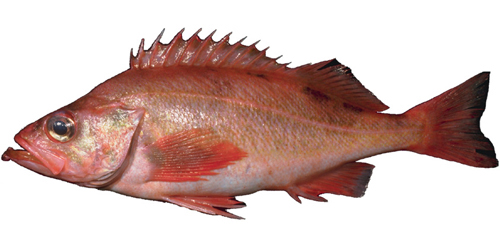
\includegraphics{Sebastes_alutus}~\\[0.5cm]
%\pdftooltip{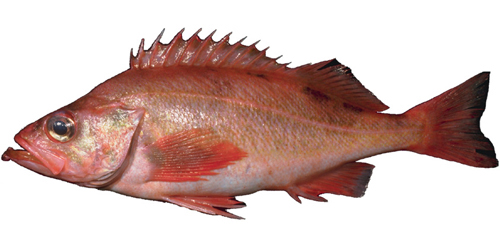
\includegraphics{Sebastes_alutus}}{This is a fish.}



Chantel R. Wetzel\textsuperscript{1}\\
Lee Cronin-Fine\textsuperscript{2}\\

\vspace{.5cm}

\small
\textsuperscript{1}Northwest Fisheries Science Center, U.S. Department of Commerce, National Oceanic and Atmospheric Administration, National Marine Fisheries Service, 2725 Montlake Boulevard East, Seattle, Washington 98112\\

\vspace{.3cm}

\textsuperscript{3}University of Washington, School of Aquatic and Fishery Sciences\\





\vspace{1cm}

\vfill
DRAFT SAFE\\
Disclaimer: This information is distributed solely for the purpose of pre-dissemination
peer review under applicable information quality guidelines. It has not been formally
disseminated by NOAA Fisheries. It does not represent and should not be construed to
represent any agency determination or policy. 

\vspace{.3cm}
%Bottom of the page
%{\large \today}

\maketitle

\pagenumbering{roman}
\setcounter{page}{1}
\end{center}

{
\setcounter{tocdepth}{4}
\tableofcontents
}
\setlength{\parskip}{5mm plus1mm minus1mm} \pagebreak

\setcounter{page}{1} \renewcommand{\thefigure}{\alph{figure}}
‼\renewcommand{\thetable}{\alph{table}}

\section*{Executive Summary}\label{executive-summary}
\addcontentsline{toc}{section}{Executive Summary}

\subsection*{Stock}\label{stock}
\addcontentsline{toc}{subsection}{Stock}

This assessment reports the status of the Pacific ocean perch
(\emph{Sebastes alutus}) species off rockfish off the U.S. West Coast
from Northern California to the Canadian Border using data through 2017.
Pacific ocean perch are most abundant in the Gulf of Alaska and have
observed off of Japan, in the Bering Sea, and south to Baja California,
although they are sparse south of Oregon and rare in southern
California. Although catches north of the US-Canada border were not
included in this assessment, it is not certain the connectivity of these
populations with contribution to the biomass possibly through adult
migration and/or larval dispersion. Composition data indicate that good
recruitment years coincide in Oregon and Washington. To date, no
significant genetic differences have been found in the range covered by
this assessment.

\subsection*{Landings}\label{landings}
\addcontentsline{toc}{subsection}{Landings}

The first year that harvest of Pacific ocean perch exceeded 1 mt off the
US West Coast first occurred in 1929. Catches ramped up in the 1940s
with large removals in Washington waters. During the 1950s the removals
primary occurred in Oregon waters with catches from Washington declining
following the 1940s. The largest removals in 1966-1968 were largely a
result of harvest by foreign vessels. The fishery proceed with more
moderate removals ranging between 1,200 to 2,600 metric tons per year
between 1969 to 1980. Removals generally declined from 1981 to 1994 to
between 1,000 and 1,700 metric tons per year. Pacific ocean perch was
declared overfished in 1999 resulting in large reduction in harvest in
recent years since the declaration. Since 2000, catches of Pacific ocean
perch have ranged between 269 - 60 mt, with catches in 2016 totaling 67
mt.

Pacific ocean perch are a desirable market species and discarding has
historically been low. However, management restrictions (e.g.~trip
limits) have resulted in increased discarding since the early 1990s.
During the 2000s discarding increased for Pacific ocean perch due to
harvest restrictions imposed to allow rebuilding, with estimated discard
rates from the bottom trawl fishery peaking in 2009 and 2010, prior to
implementation of catch shares in 2011. Since 2011, discarding of
Pacific ocean perch has been estimated to be less than 4\% given
observer data.

\begin{table}[ht]
\centering
\caption{Landings (mt) for the past 10 years for Pacific ocean perch by fleet.} 
\label{tab:Exec_catch}
\begin{tabular}{l>{\centering}p{0.7in}>{\centering}p{0.7in}>{\centering}p{0.7in}>{\centering}p{0.7in}>{\centering}p{0.7in}>{\centering}p{0.7in}}
  \hline
Year & California & Oregon & Washington & At-sea Hake & Research & Total Landings \\ 
  \hline
2007 & 0.15 & 83.65 & 45.12 & 4.05 & 0.58 & 133.55 \\ 
  2008 & 0.39 & 58.64 & 16.61 & 15.93 & 0.80 & 92.36 \\ 
  2009 & 0.92 & 58.74 & 33.22 & 1.56 & 2.72 & 97.17 \\ 
  2010 & 0.14 & 58.00 & 22.29 & 16.87 & 1.68 & 98.98 \\ 
  2011 & 0.12 & 30.26 & 19.66 & 9.17 & 1.94 & 61.14 \\ 
  2012 & 0.18 & 30.41 & 21.79 & 4.52 & 1.62 & 58.51 \\ 
  2013 & 0.08 & 34.86 & 14.83 & 5.41 & 1.71 & 56.89 \\ 
  2014 & 0.18 & 33.91 & 15.82 & 3.92 & 0.57 & 54.40 \\ 
  2015 & 0.12 & 38.05 & 11.41 & 8.71 & 1.59 & 59.88 \\ 
  2016 & 0.23 & 40.81 & 13.12 & 10.30 & 3.10 & 67.56 \\ 
   \hline
\end{tabular}
\end{table}

\FloatBarrier

\begin{figure}
\centering
\includegraphics{PacificOceanPerch2017_Assessment_files/figure-latex/unnamed-chunk-13-1.pdf}
\caption{Landings of Pacific ocean perch for California, Oregon,
Washington, the Foriegn fishery (1966-1976), At-Sea Hake fishery, and
fishery independent surveys. \label{fig:Exec_catch1}}
\end{figure}

\FloatBarrier

\subsection*{Data and Assessment}\label{data-and-assessment}
\addcontentsline{toc}{subsection}{Data and Assessment}

This a new full assessment for Pacific ocean perch which was last
assessed in 2011. In this assessment, all aspects of the model including
catches, data, and modelling assumptions were re-evaluated as much as
possible. The assessment was conducted using the length- and
age-structured modeling software Stock Synthesis (version 3.30.30.05).
The coastwide population was modeled assuming separate growth and
mortality parameters for each sex (a two-sex model) from 1918 to 2017,
and forecasted beyond 2017.

All of the sources of data for Pacific ocean perch have been
re-evaluated for 2017, excluding the historical fishery catch-per-unit
time series. Changes of varying degrees have occurred in the data from
those used in previous assessments. These current data represent the
best available scientific information. The landings history has been
updated and extended back to 1918, harvest was negligible before that
year. Survey data from the Alaska and Northwest Fisheries Science
Centers have been used to construct series of indices using a spatial
temporal delta GLMM model as well as length, age and conditional age-at
length compositions consistent with the stratifications used for
constructing the indices.

The definition of fishing fleets have been changed from those in the
2011 assessment. Three fishing fleets were specified within the model:
1) a combined bottom trawl, mid-water trawl and fixed gear fleet where
only a small fraction of Pacific ocean perch occurring by fixed gear, 2)
the historical foreign fleet, and 3) the at-sea hake fishery. The fleet
grouping were based on discarding practices. The trawl fishery estimated
a retention curve based upon discarding data and known management
restrictions. However, very little if any discarding is assumed to have
occurred by the foreign fleet and the catch reported by the at-sea hake
fishery accounts for both discarded and landed fish and hence, no
additional mortality was estimated for each of these fleets.

The assessment uses landings data and discard-fraction estimates;
catch-per-unit-of-effort and survey indices; length or age composition
data for each year and fishery or survey (with conditional age at length
compositional data for the NWFSC shelf-slope survey); information on
weight-at-age, maturity-at-age, and fecundity-at-age; priors on natural
mortality and the steepness of the Beverton-Holt stock-recruitment
relationship; and estimates of ageing error. Recruitment at
``equilibrium biomass'', length-based selectivity of the fishery and
surveys, retention of the fishery, catchability of the surveys, growth,
the time series of biomass, age and size structure, and current and
projected future stock status are outputs of the model. Natural
mortality and steepness were fixed in the final model. This was done due
to relatively flat likelihood surfaces, such that fixing parameters and
then varying them was deemed the best way to characterize uncertainty.

Although there are many types of data available for Pacific ocean perch
since the 1980s, which were used in this assessment, there is little
information about steepness and natural mortality. Estimates of
steepness are uncertain partly because of variable recruitment.
Uncertainty in natural mortality is common in many fish stock
assessments even when length and age data are available.

A number of sources of uncertainty are explicitly included in this
assessment. For example, allowance is made for uncertainty in survey
catchability coefficients. Furthermore, this assessment includes gender
differences in growth, a non-linear relationship between individual
spawner biomass and effective spawning output, and an updated
relationship between length and maturity, based upon non-published
information (M. Head, personal communication). As is always the case,
overall uncertainty is greater than that predicted by a single model
specification. Among other sources of uncertainty that are not included
in the current model are the degree of connectivity between the stocks
of Pacific ocean perch off of Vancouver Island, British Columbia and
those in PFMC waters, and the effect of climatic variables on
recruitment, growth and survival of Pacific ocean perch.

A reference case was selected which adequately captures the central
tendency for those sources of uncertainty considered in the model.

\subsection*{Stock Biomass}\label{stock-biomass}
\addcontentsline{toc}{subsection}{Stock Biomass}

The predicted spawning biomass from the base model generally showed a
slight decline over the time series until 1966 when the foreign fleet
began. A short, but sharp decline occurred, followed by a period of the
stock biomass stabilizing or with a minimal decline until the late
1990s. The stock showed increases in stock size following the year 2000
when a combination of strong recruitment and low catches resulted. The
2017 spawning biomass relative to unfished equilibrium spawning biomass
is above the target of 40\% of unfished spawning biomass at 2017 is
76.1\% (\textasciitilde{}95\% asymptotic interval: \(\pm\)
53.8\%-98.4\%)\%. Approximate confidence intervals based on the
asymptotic variance estimates show that the uncertainty in the estimated
spawning biomass is high.

\begin{figure}
\centering
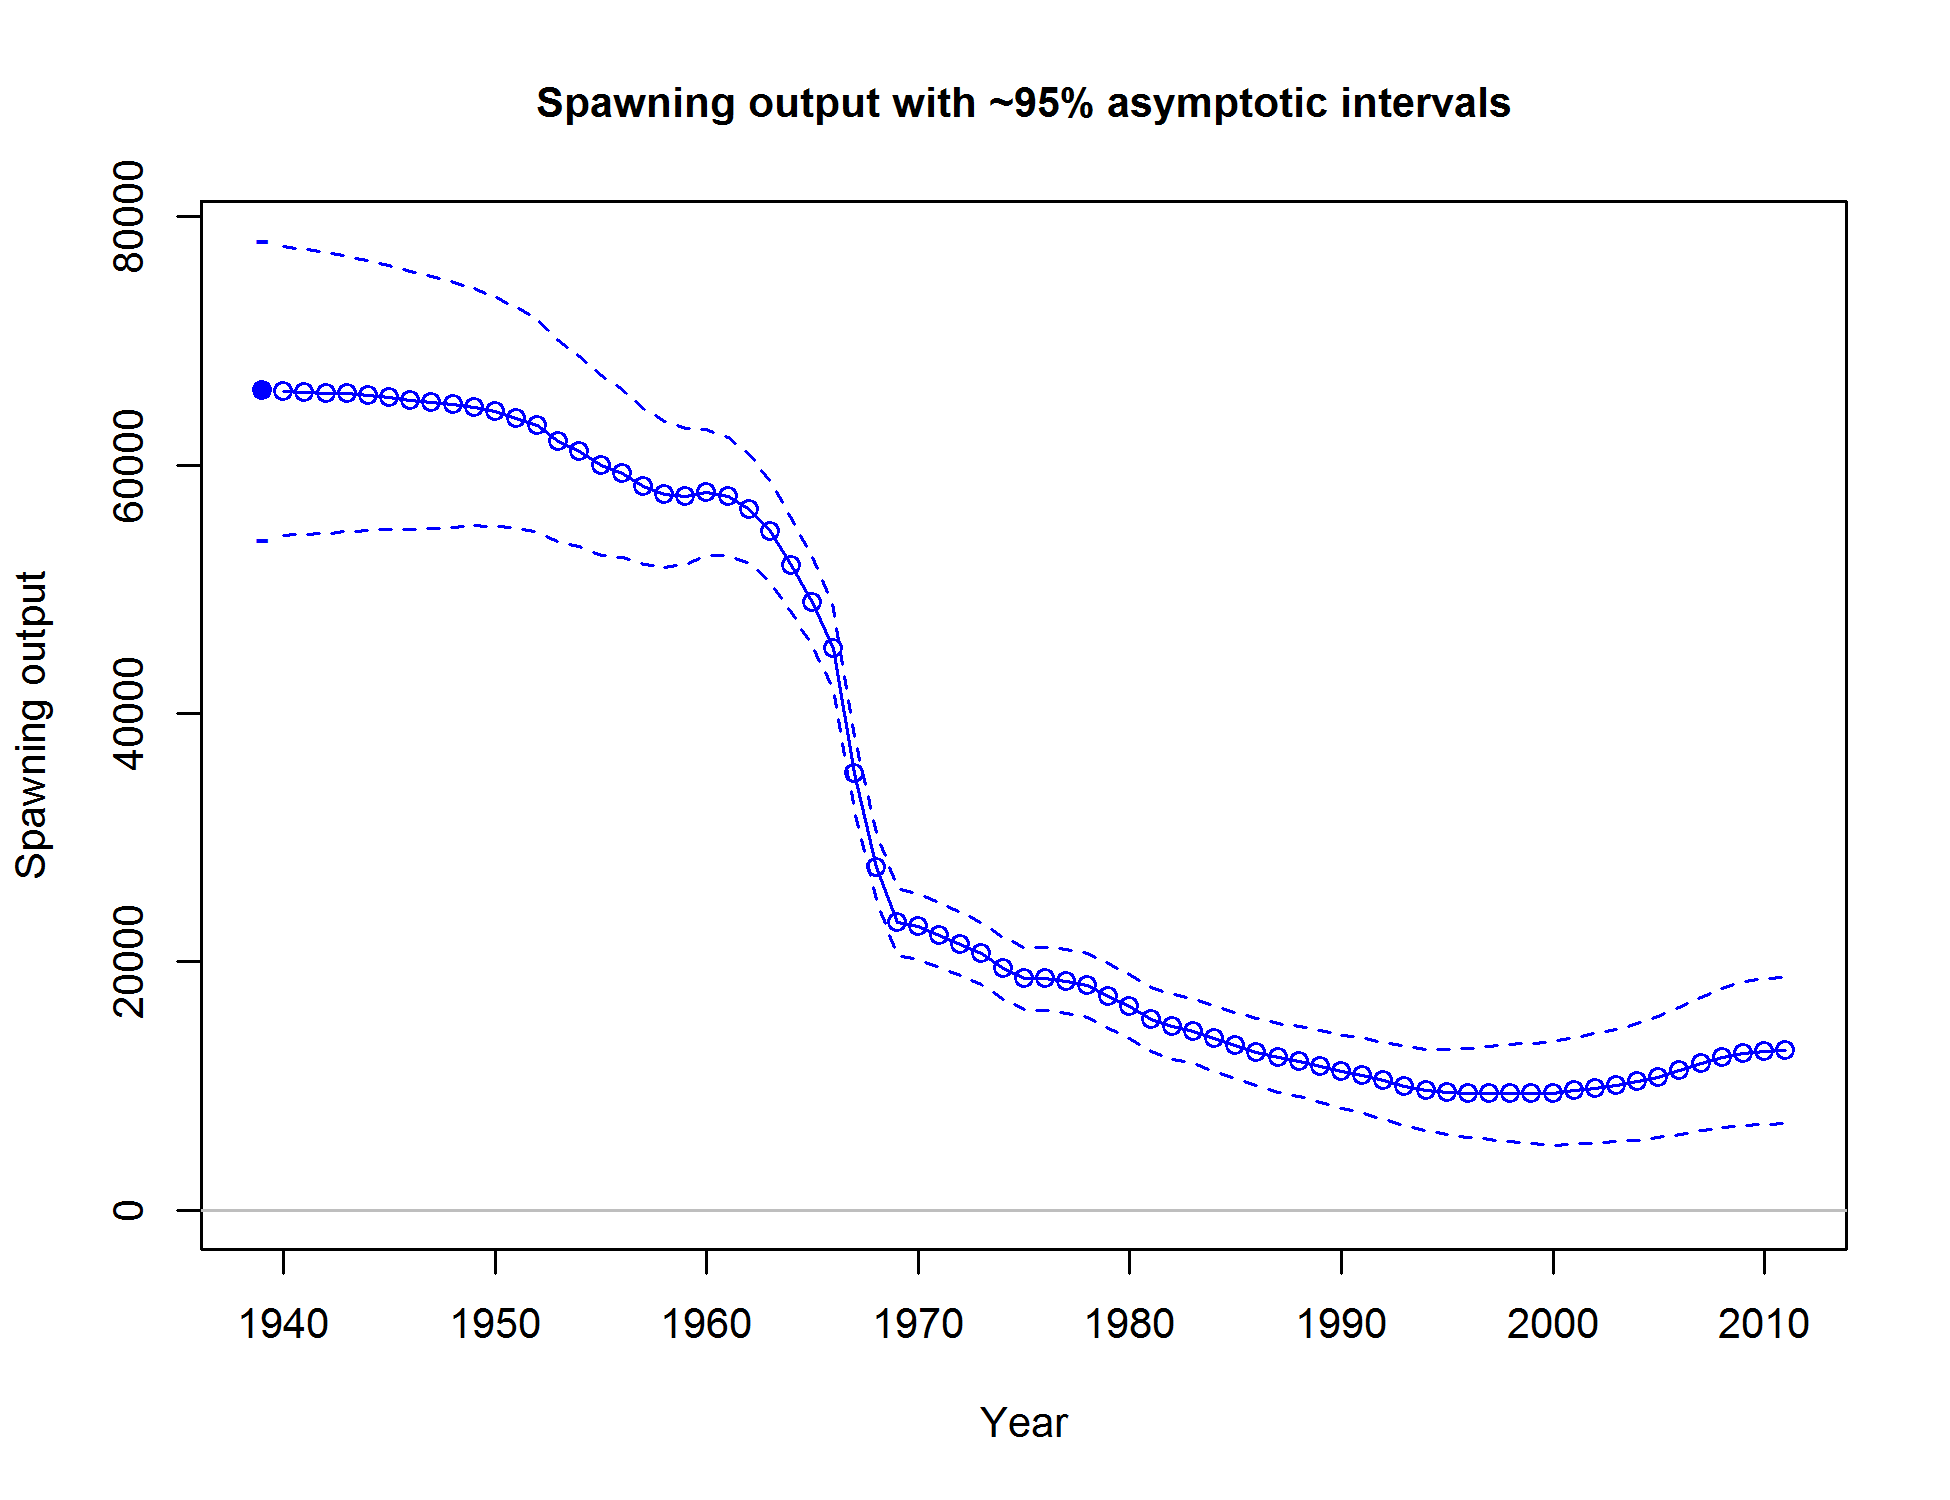
\includegraphics{r4ss/plots_mod1/ts7_Spawning_output_with_95_asymptotic_intervals_intervals.png}
\caption{Time series of spawning output trajectory (circles and line:
median; light broken lines: 95\% credibility intervals) for the base
case assessment model. \label{fig:Spawnbio_all}}
\end{figure}

\begin{figure}
\centering
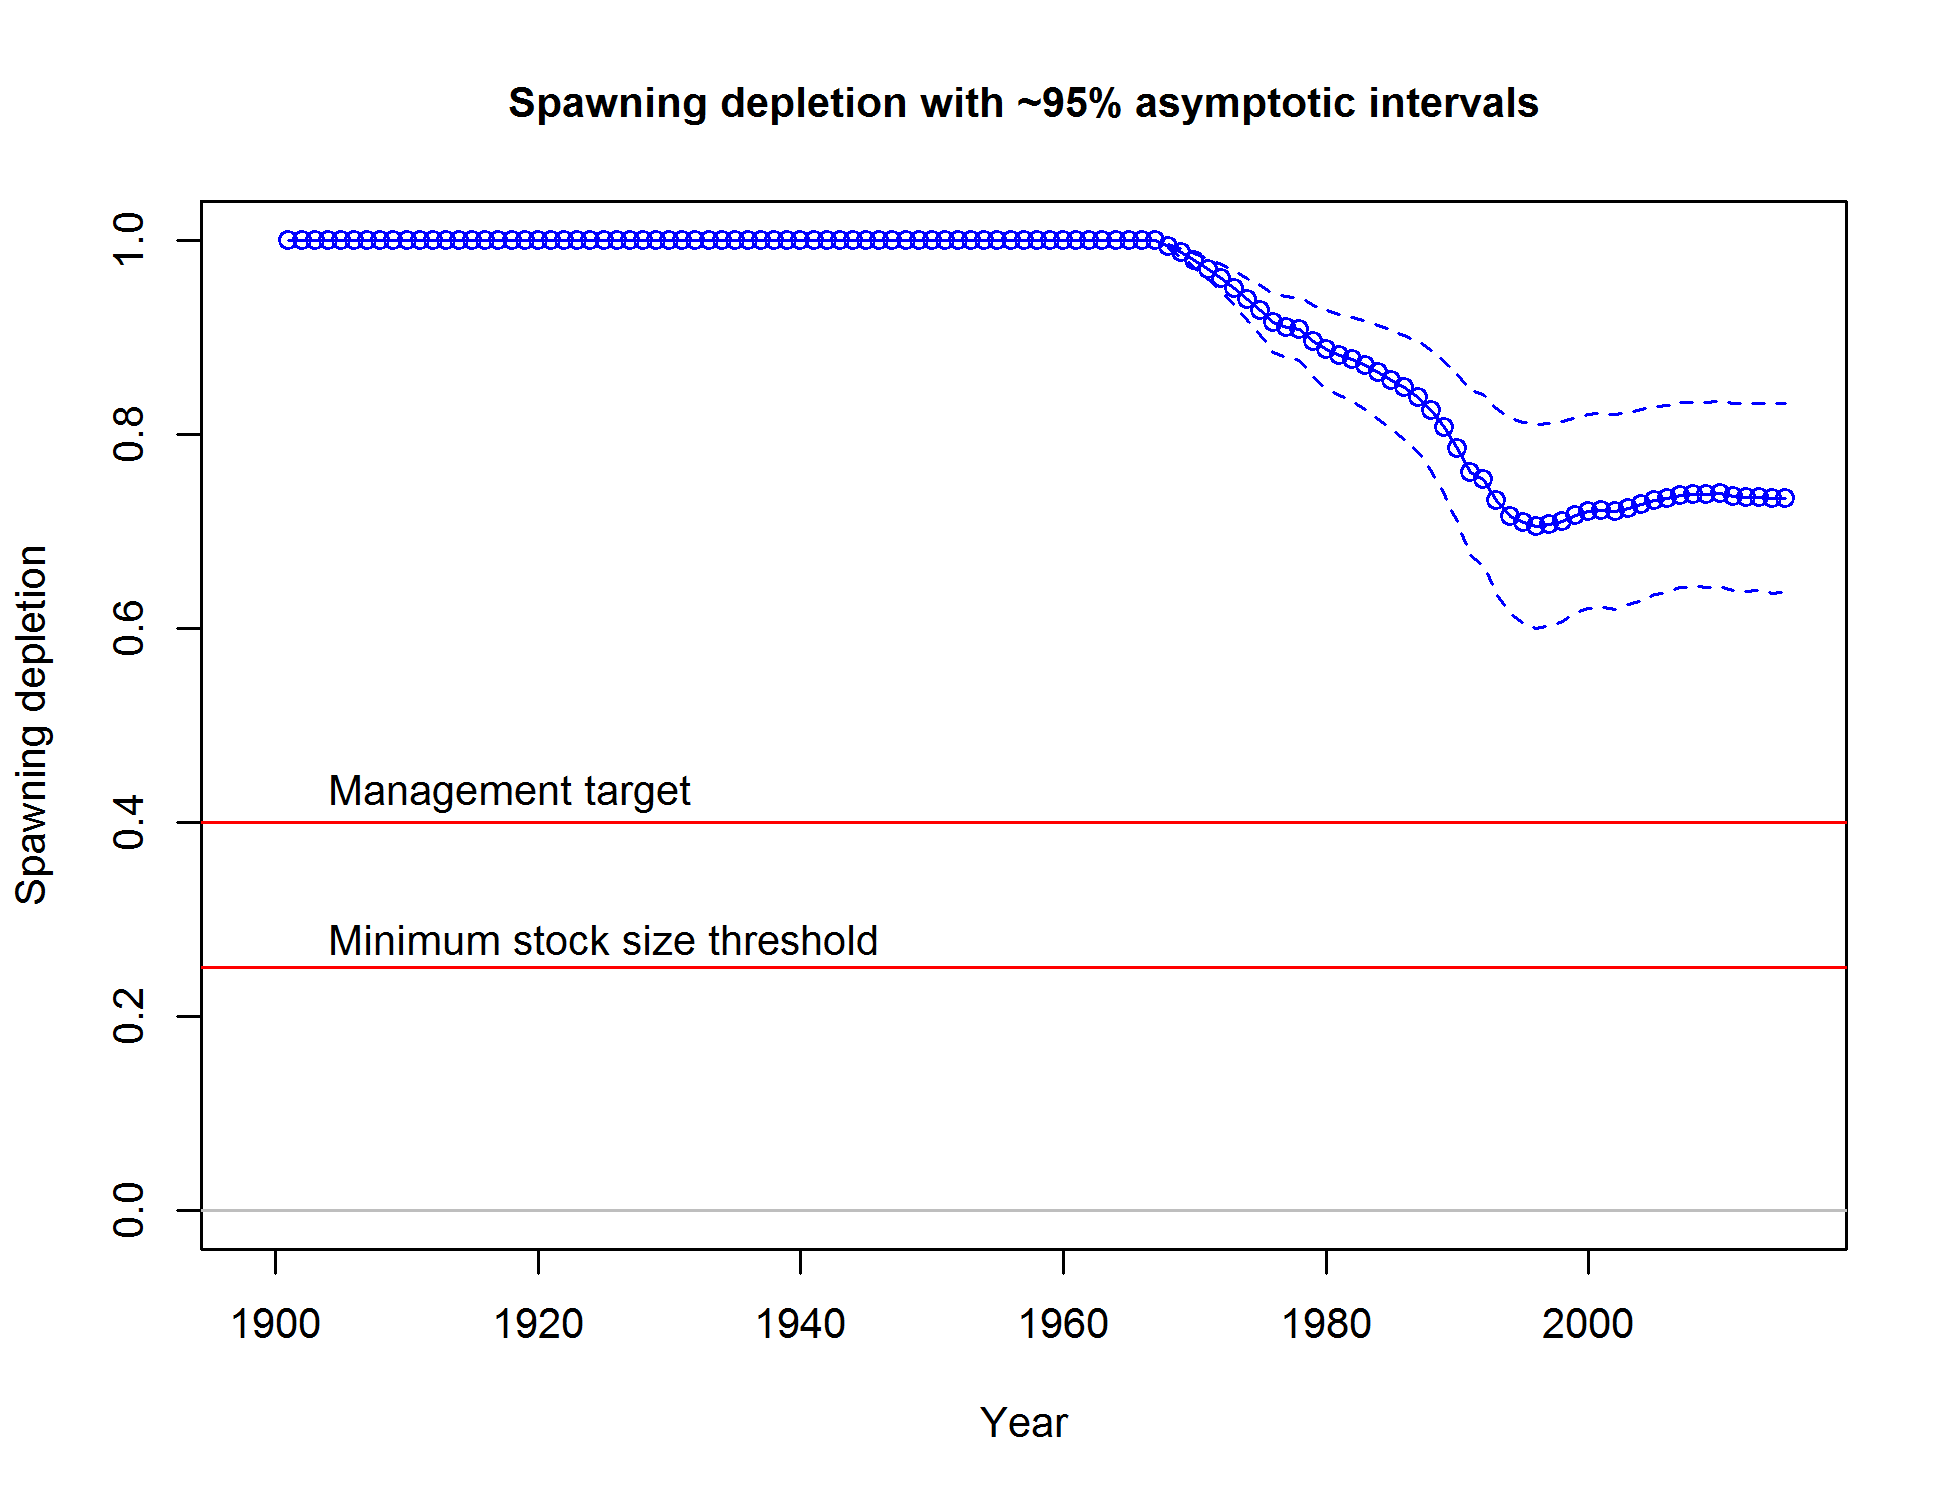
\includegraphics{r4ss/plots_mod1/ts9_Spawning_depletion_with_95_asymptotic_intervals_intervals.png}
\caption{Estimated relative spawning biomass (depletion) with
approximate 95\% asymptotic confidnce intervals (dashed lines) for the
base case assessment model. \label{fig:RelDeplete_all}}
\end{figure}

\begin{table}[ht]
\centering
\caption{Recent trend in estimated spawning output (million eggs) and relative spawning output.} 
\label{tab:SpawningDeplete_mod1}
\begin{tabular}{l>{\centering}p{1.3in}>{\centering}p{1.2in}>{\centering}p{1in}>{\centering}p{1.2in}}
  \hline
Year & Spawning Output (million eggs) & \~{} 95\% confidence interval & Estimated depletion & \~{} 95\% confidence interval \\ 
  \hline
2008 & 3211.00 & 1362 - 5060 & 0.48 & 0.330 - 0.638 \\ 
  2009 & 3346.00 & 1425 - 5267 & 0.50 & 0.345 - 0.664 \\ 
  2010 & 3438.00 & 1467 - 5408 & 0.52 & 0.355 - 0.681 \\ 
  2011 & 3500.00 & 1496 - 5504 & 0.53 & 0.362 - 0.693 \\ 
  2012 & 3545.00 & 1521 - 5570 & 0.53 & 0.368 - 0.701 \\ 
  2013 & 3584.00 & 1544 - 5625 & 0.54 & 0.373 - 0.708 \\ 
  2014 & 3727.00 & 1618 - 5835 & 0.56 & 0.390 - 0.733 \\ 
  2015 & 4118.00 & 1812 - 6425 & 0.62 & 0.435 - 0.807 \\ 
  2016 & 4620.00 & 2054 - 7186 & 0.70 & 0.491 - 0.902 \\ 
  2017 & 5047.00 & 2259 - 7835 & 0.76 & 0.538 - 0.984 \\ 
   \hline
\end{tabular}
\end{table}

\FloatBarrier

\subsection*{Recruitment}\label{recruitment}
\addcontentsline{toc}{subsection}{Recruitment}

Recruitment deviations were estimated for the entire time-series
modeled. There is little information regarding recruitment prior to
1965, and the uncertainty in these estimates is expressed in the model.
Historically, there are estimates of large recruitments in 1999 and
2000. In recent years, a recruitment of unprecedented size is estimated
to have occurred in 2008 but is highly uncertain. Additionally, there is
early evidence of a strong recruitment in 2013. The four lowest
recruitments (in ascending order) occurred in 2012, 2003, 1998, and
2005.

\begin{figure}
\centering
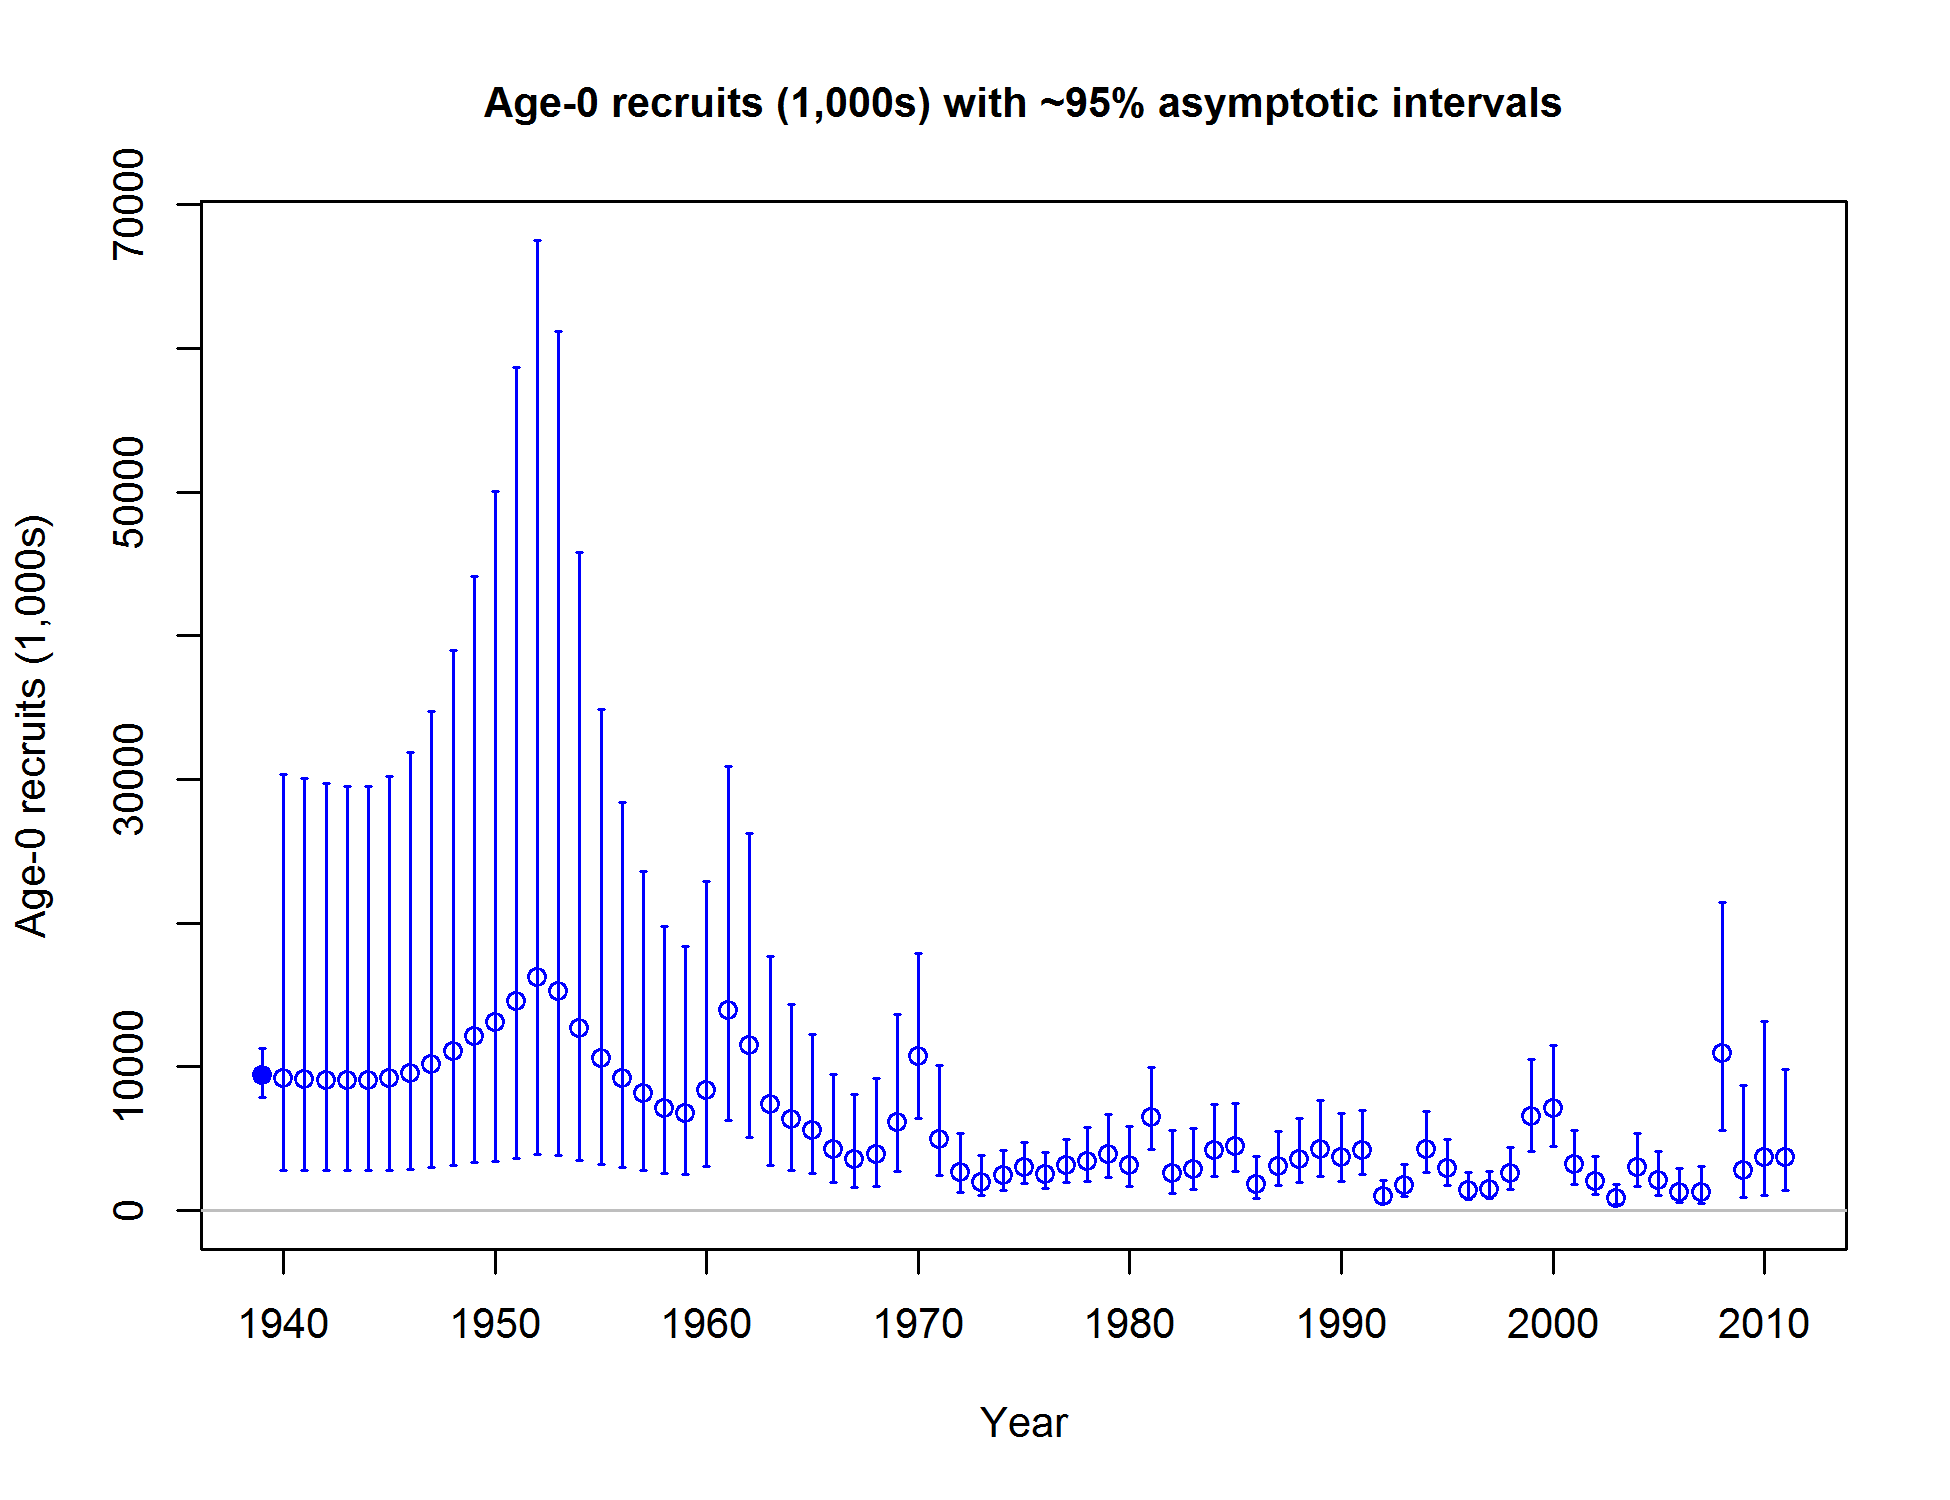
\includegraphics{r4ss/plots_mod1/ts11_Age-0_recruits_(1000s)_with_95_asymptotic_intervals.png}
\caption{Time series of estimated Pacific ocean perch recruitments for
the base-case model with 95\% confidence or credibility intervals.
\label{fig:Recruits_all}}
\end{figure}

\begin{table}[ht]
\centering
\caption{Recent estimated trend in recruitment with approximate 95/% 
                                        confidence intervals determined from the base model} 
\label{tab:Recruit_mod1}
\begin{tabular}{>{\centering}p{.8in}>{\centering}p{1.0in}>{\centering}p{1.4in}>{\centering}p{1.0in}>{\centering}p{1.4in}}
  \hline
Year & Estimated Recruitment & \~{} 95\% confidence interval & Estimated Recruitment Devs. & \~{} 95\% confidence interval \\ 
  \hline
2008 & 133246.00 & 75744 - 234402 & 2.84 & 2.542 - 3.145 \\ 
  2009 & 4814.00 & 2070 - 11196 & -0.49 & -1.254 - 0.267 \\ 
  2010 & 8279.00 & 4007 - 17102 & 0.04 & -0.558 - 0.633 \\ 
  2011 & 16107.00 & 8067 - 32159 & 0.70 & 0.146 - 1.246 \\ 
  2012 & 2113.00 & 870 - 5132 & -1.34 & -2.173 - -0.507 \\ 
  2013 & 29278.00 & 13512 - 63442 & 1.20 & 0.525 - 1.872 \\ 
  2014 & 5078.00 & 1728 - 14918 & -0.65 & -1.748 - 0.441 \\ 
  2015 & 10096.00 & 2827 - 36059 & -0.00 & -1.372 - 1.367 \\ 
  2016 & 10520.00 & 2945 - 37581 & 0.00 & -1.372 - 1.372 \\ 
  2017 & 10816.00 & 3031 - 38596 & 0.00 & -1.372 - 1.372 \\ 
   \hline
\end{tabular}
\end{table}

\FloatBarrier

\subsection*{Exploitation status}\label{exploitation-status}
\addcontentsline{toc}{subsection}{Exploitation status}

The spawning biomass of Pacific ocean perch reached a low in 1994.
Catches for Pacific ocean perch decreased significantly in 2000 compared
to previous years. The estimated relative biomass was possibly below the
overfished level in the early 2000s, but has likely remained above that
level otherwise, and currently is significantly greater than the 40\%
unfished spawning biomass target. Throughout the late 1960s and 1970s
the exploitation rate and (1-SPR)/(1-SPR\textsubscript{50\%}) were
mostly above target levels. Recent exploitation rates on Pacific ocean
perch were predicted to be significantly below target levels.

\begin{table}[ht]
\centering
\caption{Recent trend in spawning potential 
                                        ratio (1-SPR) and summary exploitation rate for Pacific ocean perch.} 
\label{tab:SPR_Exploit_mod1}
\begin{tabular}{l>{\centering}p{1in}>{\centering}p{1.2in}>{\centering}p{1in}>{\centering}p{1.2in}}
  \hline
Year & (1-SPR) & \~{} 95\% confidence interval & Exploitation rate & \~{} 95\% confidence interval \\ 
  \hline
2007 & 0.104 & 0.046 - 0.162 & 0.002 & 0.001 - 0.003 \\ 
  2008 & 0.086 & 0.036 - 0.135 & 0.002 & 0.001 - 0.003 \\ 
  2009 & 0.113 & 0.046 - 0.181 & 0.003 & 0.001 - 0.004 \\ 
  2010 & 0.107 & 0.044 - 0.171 & 0.002 & 0.001 - 0.004 \\ 
  2011 & 0.037 & 0.016 - 0.058 & 0.001 & 0.000 - 0.001 \\ 
  2012 & 0.035 & 0.015 - 0.054 & 0.001 & 0.000 - 0.001 \\ 
  2013 & 0.033 & 0.014 - 0.051 & 0.001 & 0.000 - 0.001 \\ 
  2014 & 0.029 & 0.013 - 0.045 & 0.001 & 0.000 - 0.001 \\ 
  2015 & 0.028 & 0.013 - 0.044 & 0.001 & 0.000 - 0.001 \\ 
  2016 & 0.028 & 0.012 - 0.043 & 0.001 & 0.000 - 0.001 \\ 
   \hline
\end{tabular}
\end{table}

\FloatBarrier

\begin{figure}
\centering
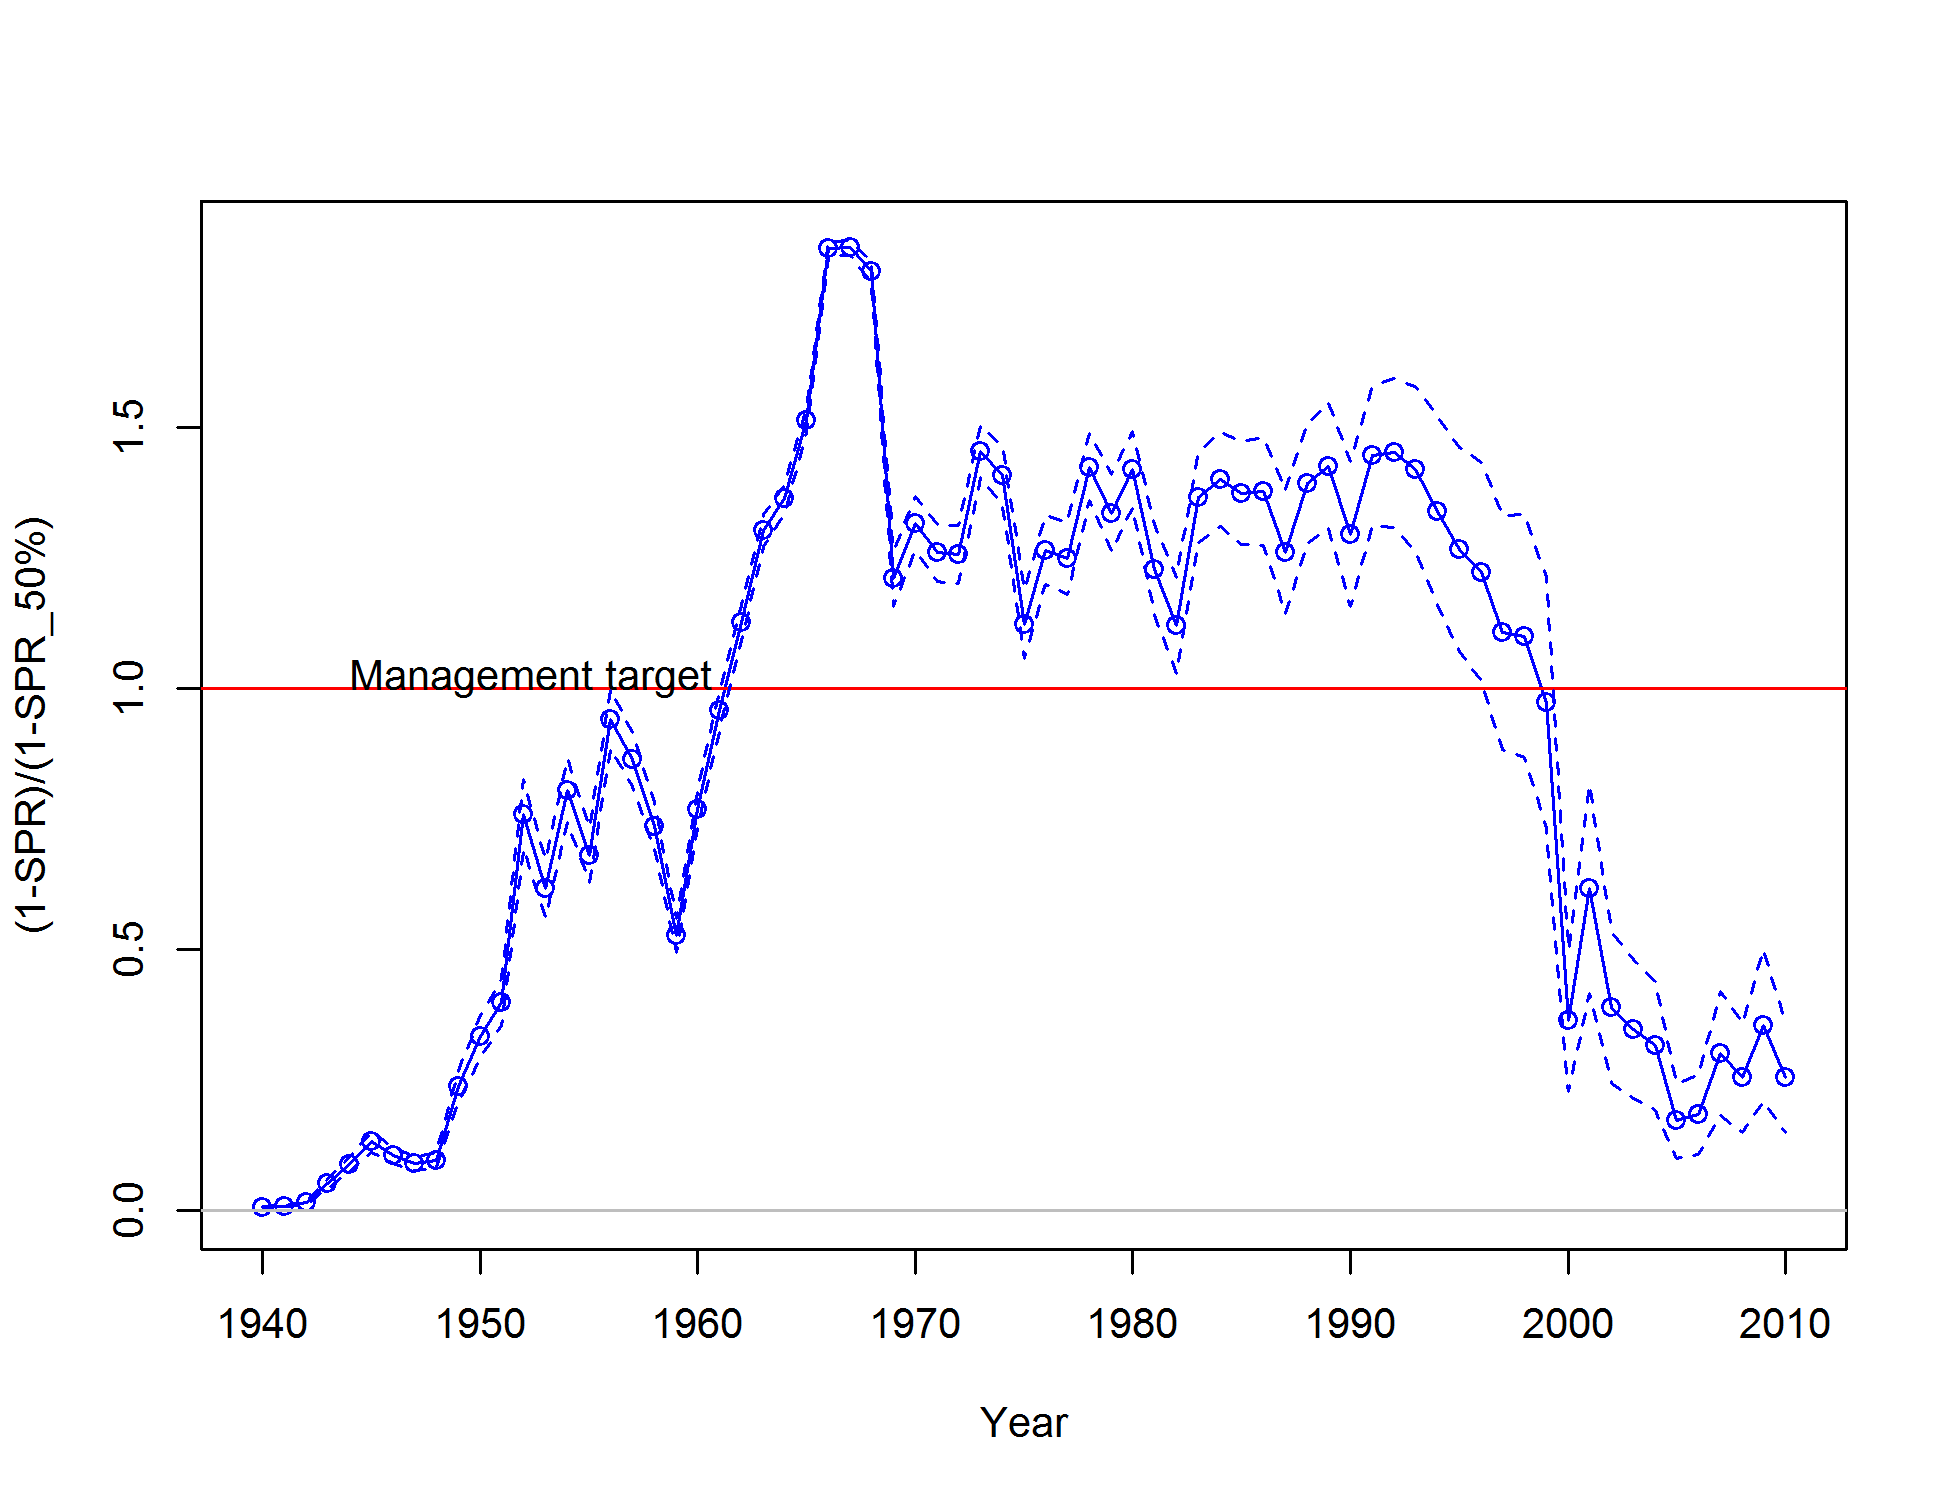
\includegraphics{r4ss/plots_mod1/SPR3_ratiointerval.png}
\caption{Estimated spawning potential ratio (1-SPR)/(1-SPR50\%) for the
base-case model. One minus SPR is plotted so that higher exploitation
rates occur on the upper portion of the y-axis. The management target is
plotted as a red horizontal line and values above this reflect harvests
in excess of the overfishing proxy based on the SPR50\% harvest rate.
The last year in the time series is 2016. \label{fig:SPR_all}}
\end{figure}

\begin{figure}
\centering
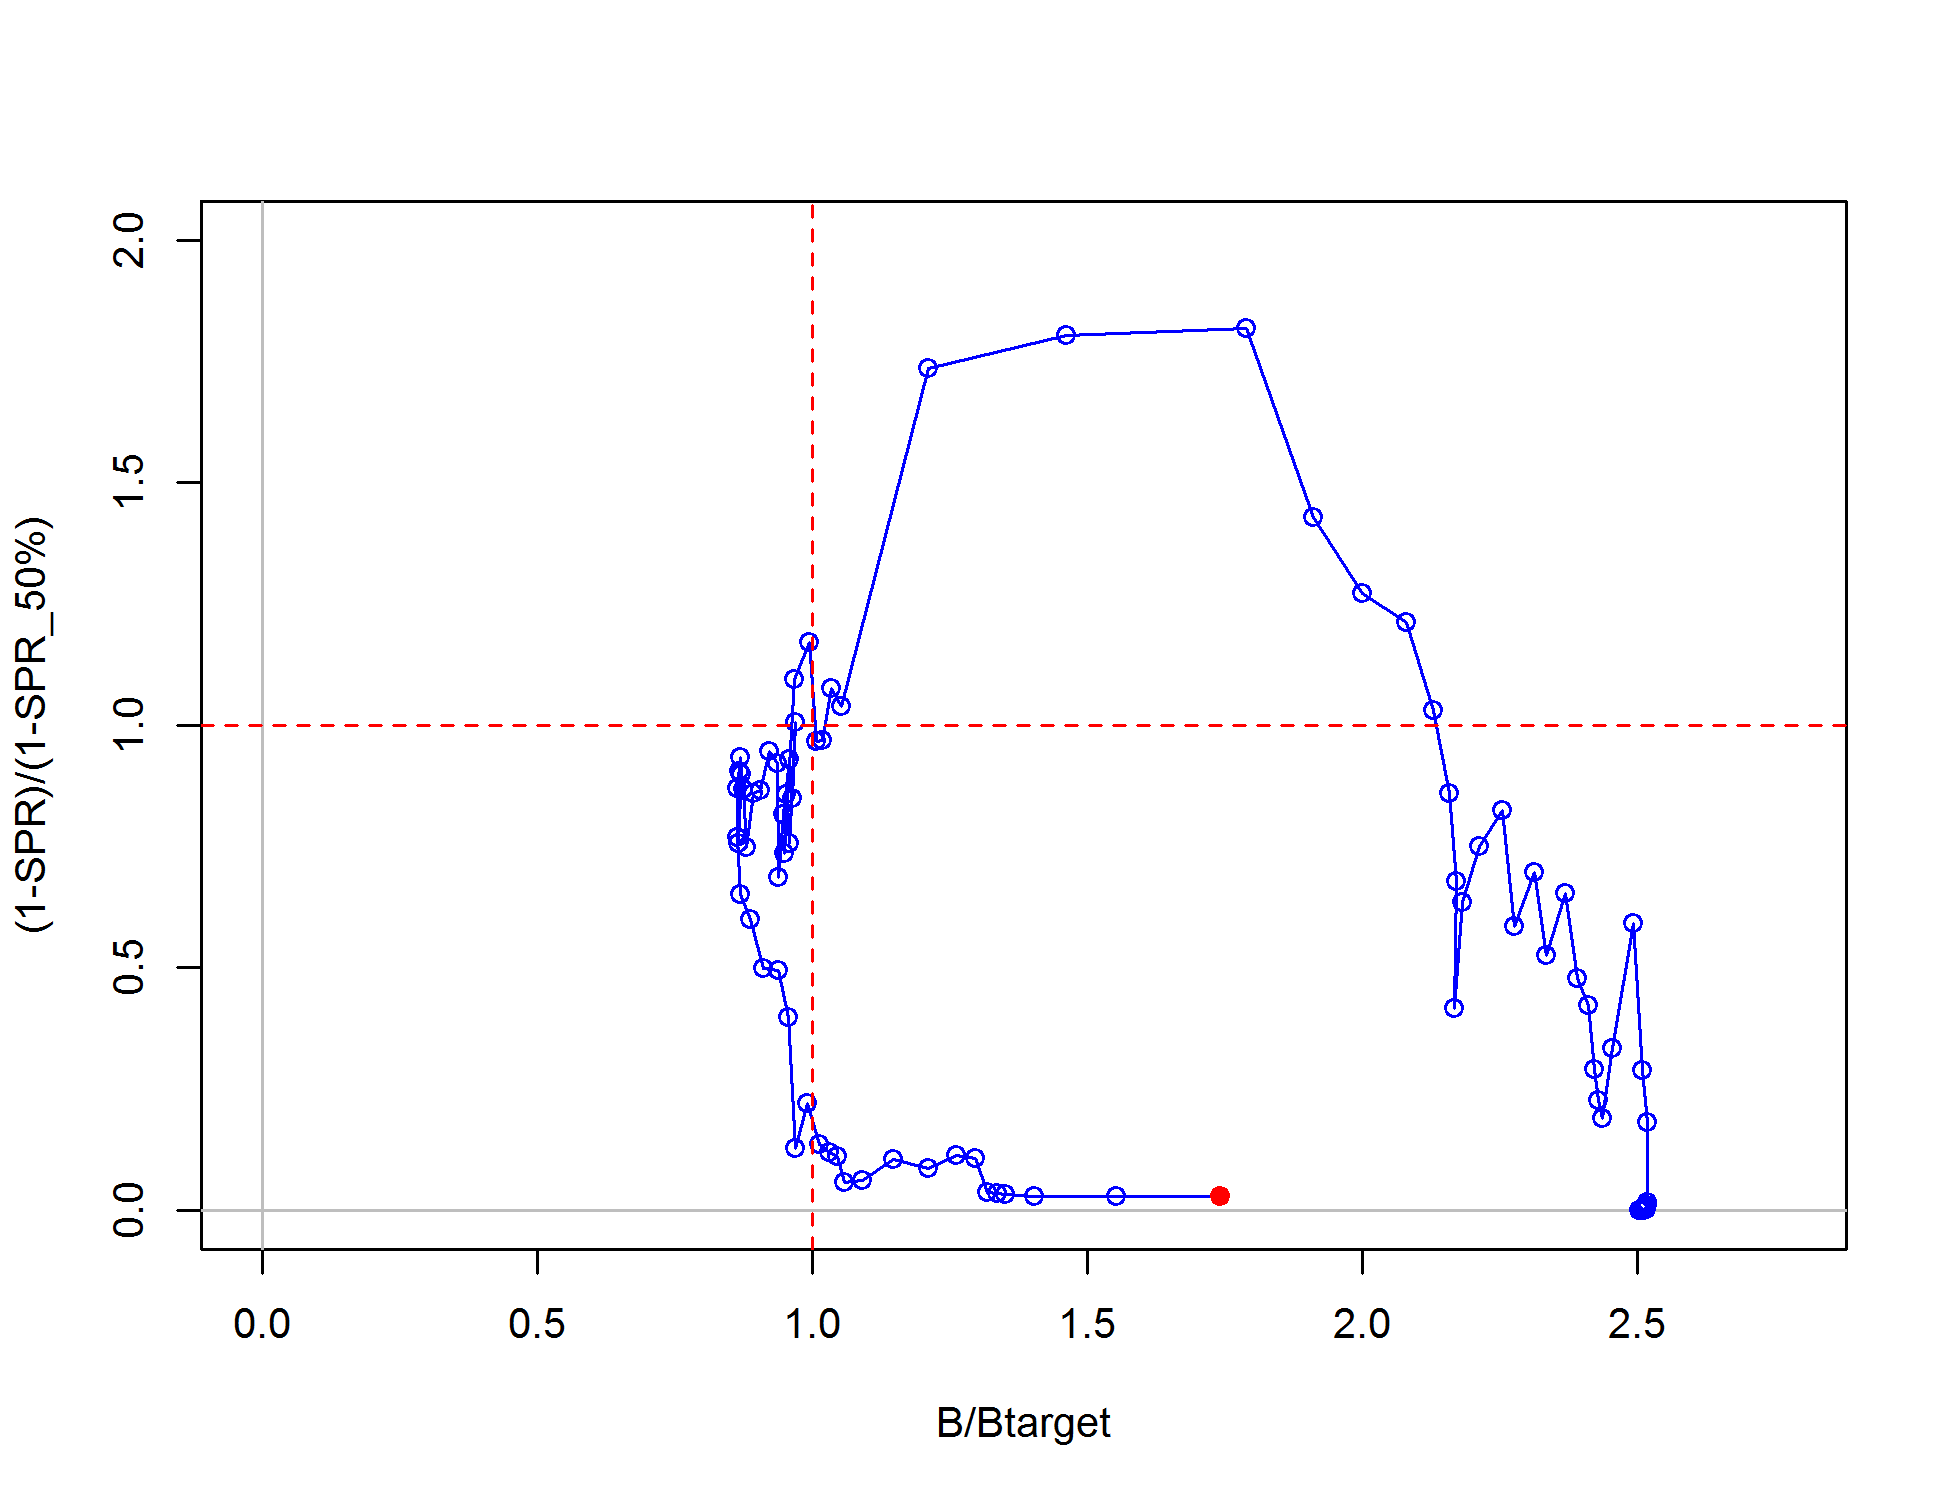
\includegraphics{r4ss/plots_mod1/SPR4_phase.png}
\caption{Phase plot of estimated relative (1-SPR)/(1-SPR50\%)
vs.~relative spawning biomass for the base case model. Relative biomass
is the annual spawning biomass divided by the unfished spawning biomass.
\label{fig:Phase_all}}
\end{figure}

\FloatBarrier

\subsection*{Ecosystem Considerations}\label{ecosystem-considerations}
\addcontentsline{toc}{subsection}{Ecosystem Considerations}

Rockfish are an important component of the California Current ecosystem
along the US west coast, with its more than sixty five species filling
various niches in both soft and hard bottom habitats from the nearshore
to the continental slope, as well as near bottom and pelagic zones.
Pacific ocean perch are generally considered to be semi-demersal but,
there can at times, be a significant pelagic component to their
distribution.

Recruitment is one mechanism by which the ecosystem may directly impact
the population dynamics of Pacific ocean perch. The 1999 cohort for many
species of rockfish was large - sometimes significantly so - from these
species' long-term averages suggesting that environmental conditions may
influence the spawning success and survival of larvae and juvenile
rockfish. Pacific ocean perch showed an above average recruitment
deviation in 1999 and 2000, but absolute recruitment was not as large as
other years. The specific pathways through which environmental
conditions exert influence on Pacific ocean perch dynamics are unclear;
however, changes in water temperature and currents, distribution of prey
and predators, and the amount and timing of upwelling are all possible
linkages. Changes in the environment may also result in changes in
age-at-maturity, fecundity, growth, and survival which can affect how
the status of the stock and its susceptibility to fishing are
determined. Unfortunately, there are few data available for Pacific
ocean perch that provide insights into these effects.

Fishing has effects on both the age structure of a population as well as
the habitat with which the target species is associated. Fishing often
targets larger, older fish, and years of fishing mortality results in a
truncated age-structure when compared to unfished conditions. Rockfish
are often associated with habitats containing living structure such as
sponges and corals, and fishing may alter that habitat to a less
desirable state. This assessment provides a look at the effects of
fishing on age structure, and recent studies on essential fish habitat
are beginning to characterize important locations for rockfish
throughout their life history; however there is little current
information available to evaluate the specific effects of fishing on the
ecosystem issues specific to Pacific ocean perch.

\subsection*{Reference Points}\label{reference-points}
\addcontentsline{toc}{subsection}{Reference Points}

This stock assessment estimates that Pacific ocean perch in the base
model are above the biomass target. Due to the large 2008 year-class, an
increasing trend in spawning biomass was estimated in the base model.
The estimated relative biomass level in 2017 is 76.1\%
(\textasciitilde{}95\% asymptotic interval: \(\pm\) 53.8\%-98.4\%),
corresponding to an unfished spawning output of 5047 million eggs
(\textasciitilde{}95\% asymptotic interval: 2259-7835 million eggs) of
spawning output in the base model. Unfished age 3+ biomass was estimated
to be 139810 mt in the base case model. The target spawning output based
on the biomass target (\(SB_{40\%}\)) is 2653.2 million eggs, which
gives a catch of 1748.2 mt. Equilibrium yield at the proxy \(F_{MSY}\)
harvest rate corresponding to \(SPR_{50\%}\) is 1764.8 mt.

\begin{table}[ht]
\centering
\caption{Summary of reference 
                                      points and management quantities for the 
                                      base case.} 
\label{tab:Ref_pts_mod1}
\begin{tabular}{>{\raggedright}p{4.1in}>{\centering}p{.65in}>{\centering}p{1.4in}}
  \hline
\textbf{Quantity} & \textbf{Estimate} & \textbf{\~95\%  Confidence Interval} \\ 
  \hline
Unfished spawning output (million eggs) & 6633.1 &   4736.7 -   8529.5 \\ 
  Unfished age 3+ biomass (mt) & 139810 & 100052.5 - 179567.5 \\ 
  Unfished recruitment (R0, thousands) & 11665.7 &   8801.4 -  15462.1 \\ 
  Spawning output(2017 million eggs) & 5047.2 &   2259.2 -   7835.1 \\ 
  Depletion (2017) & 0.761 &    0.538 -    0.984 \\ 
  \textbf{$\text{Reference points based on } \mathbf{SB_{40\%}}$} &  &  \\ 
  Proxy spawning output ($B_{40\%}$) & 2653.2 &   1894.7 -   3411.8 \\ 
  SPR resulting in $B_{40\%}$ ($SPR_{B40\%}$) & 0.55 &     0.55 -     0.55 \\ 
  Exploitation rate resulting in $B_{40\%}$ & 0.028 &    0.028 -    0.029 \\ 
  Yield with $SPR_{B40\%}$ at $B_{40\%}$ (mt) & 1748.2 &   1252.4 -     2244 \\ 
  \textbf{\textit{Reference points based on SPR proxy for MSY}} &  &  \\ 
  Spawning output & 2211 &   1578.9 -   2843.2 \\ 
  $SPR_{proxy}$ & 0.5 &  \\ 
  Exploitation rate corresponding to $SPR_{proxy}$ & 0.034 &    0.033 -    0.034 \\ 
  Yield with $SPR_{proxy}$ at $SB_{SPR}$ (mt) & 1764.8 &   1264.8 -   2264.8 \\ 
  \textbf{\textit{Reference points based on estimated MSY values}} &  &  \\ 
  Spawning output at $MSY$ ($SB_{MSY}$) & 2315.7 &   1649.6 -   2981.8 \\ 
  $SPR_{MSY}$ & 0.512 &     0.51 -    0.514 \\ 
  Exploitation rate at $MSY$ & 0.032 &    0.032 -    0.033 \\ 
  $MSY$ (mt)  & 1766.7 &   1266.1 -   2267.4 \\ 
   \hline
\end{tabular}
\end{table}

\FloatBarrier

\subsection*{Management Performance}\label{management-performance}
\addcontentsline{toc}{subsection}{Management Performance}

Exploitation rates on Pacific ocean perch exceeded MSY proxy target
harvest rates during the 1960s and 1970s and spawning biomass is
predicted to have fallen below the proxy management target of 40\%.
Exploitation rates subsequently declined to rates at or below the
management target in the 1980s. Management restrictions imposed in the
1990s further reduced exploitation rates. An overfished declaration for
Pacific ocean perch resulted in very low exploitation rates since 2001
with the ACLs being set far below the OFL and ABC values.

\begin{table}[ht]
\centering
\caption{Recent trend in total catch and commercial 
                              landings (mt) relative to the management guidelines. 
                              Estimated total catch reflect the commercial landings 
                              plus the model estimated discarded biomass.} 
\label{tab:mnmgt_perform}
\scalebox{0.9}{
\begin{tabular}{>{\raggedleft}p{0.5in}>{\centering}p{1.1in}>{\centering}p{1.1in}>{\centering}p{1.1in}>{\centering}p{1.1in}>{\centering}p{1.1in}}
  \hline
Year & OFL (mt; ABC prior to 2011) & ABC (mt) & ACL (mt; OY prior to 2011) & Total landings (mt) & Estimated total catch (mt) \\ 
  \hline
\text{2007} & 900 &  & 150 & 133 & 157 \\ 
  \text{2008} & 911 &  & 150 & 92 & 133 \\ 
  \text{2009} & 1,160 &  & 189 & 94 & 190 \\ 
  \text{2010} & 1,173 &  & 200 & 97 & 181 \\ 
  \text{2011} & 1,026 & 981 & 180 & 60 & 61 \\ 
  \text{2012} & 1,007 & 962 & 183 & 57 & 58 \\ 
  \text{2013} & 844 & 807 & 150 & 55 & 57 \\ 
  \text{2014} & 838 & 801 & 153 & 54 & 55 \\ 
  \text{2015} & 842 & 805 & 158 & 58 & 59 \\ 
  \text{2016} & 850 & 813 & 164 & 65 & 65 \\ 
   \hline
\end{tabular}
}
\end{table}

\FloatBarrier

\subsection*{Unresolved Problems And Major
Uncertainties}\label{unresolved-problems-and-major-uncertainties}
\addcontentsline{toc}{subsection}{Unresolved Problems And Major
Uncertainties}

TBD after STAR panel

\subsection*{Decision Table}\label{decision-table}
\addcontentsline{toc}{subsection}{Decision Table}

TBD after STAR panel

\begin{table}[ht]
\centering
\caption{Projections of potential OFL (mt) and ACL (mt) and the estimated spawning output and relative biomass.} 
\label{tab:OFL_projection}
\begin{tabular}{>{\raggedleft}p{0.5in}>{\centering}p{1.1in}>{\centering}p{1.1in}>{\centering}p{1.6in}>{\centering}p{1.1in}}
  \hline
Year & OFL & ACL & Spawning Output ( million eggs ) & Relative Biomass \\ 
  \hline
2017 & 4306 & 281 & 5047 & 0.761 \\ 
  2018 & 4559 & 281 & 5369 & 0.809 \\ 
  2019 & 4719 & 4515 & 5625 & 0.848 \\ 
  2020 & 4654 & 4453 & 5657 & 0.853 \\ 
  2021 & 4552 & 4356 & 5654 & 0.852 \\ 
  2022 & 4431 & 4240 & 5606 & 0.845 \\ 
  2023 & 4302 & 4116 & 5528 & 0.833 \\ 
  2024 & 4172 & 3992 & 5431 & 0.819 \\ 
  2025 & 4048 & 3873 & 5324 & 0.803 \\ 
  2026 & 3932 & 3762 & 5211 & 0.786 \\ 
  2027 & 3826 & 3660 & 5096 & 0.768 \\ 
  2028 & 3727 & 3566 & 4981 & 0.751 \\ 
   \hline
\end{tabular}
\end{table}

\FloatBarrier

\begin{table}[ht]
\centering
\caption{Summary of 10-year 
                                             projections beginning in 2019 
                                             for alternate states of nature based on 
                                             an axis of uncertainty for the base model. 
                                             Columns range over low, mid, and high
                                             states of nature, and rows range over different 
                                             assumptions of catch levels. An entry of "--" 
                                             indicates that the stock is driven to very low 
                                             abundance under the particular scenario.} 
\label{tab:Decision_table_mod1}
\scalebox{0.85}{
\begin{tabular}{l|cc|>{\centering}p{.7in}c|>{\centering}p{.7in}c|>{\centering}p{.7in}c}
   \multicolumn{3}{c}{}  &  \multicolumn{2}{c}{} 
                               & \multicolumn{2}{c}{\textbf{States of nature}} 
                               & \multicolumn{2}{c}{} \\
  \multicolumn{3}{c}{}  &  \multicolumn{2}{c}{Low State of Nature} 
                               & \multicolumn{2}{c}{Base State of Nature} 
                               &  \multicolumn{2}{c}{High State of Nature} \\
 \hline
 & Year & Catch & Spawning Output & Depletion & Spawning Output & Depletion & Spawning Output & Depletion \\ 
  \hline
 & 2019 & - & - & - & - & - & - & - \\ 
   & 2020 & - & - & - & - & - & - & - \\ 
   & 2021 & - & - & - & - & - & - & - \\ 
  Catch Option 1 & 2022 & - & - & - & - & - & - & - \\ 
   & 2023 & - & - & - & - & - & - & - \\ 
   & 2024 & - & - & - & - & - & - & - \\ 
   & 2025 & - & - & - & - & - & - & - \\ 
   & 2026 & - & - & - & - & - & - & - \\ 
   & 2027 & - & - & - & - & - & - & - \\ 
   & 2028 & - & - & - & - & - & - & - \\ 
   \hline
 & 2019 & - & - & - & - & - & - & - \\ 
   & 2020 & - & - & - & - & - & - & - \\ 
   & 2021 & - & - & - & - & - & - & - \\ 
  Catch Option 2 & 2022 & - & - & - & - & - & - & - \\ 
   & 2023 & - & - & - & - & - & - & - \\ 
   & 2024 & - & - & - & - & - & - & - \\ 
   & 2025 & - & - & - & - & - & - & - \\ 
   & 2026 & - & - & - & - & - & - & - \\ 
   & 2027 & - & - & - & - & - & - & - \\ 
   & 2028 & - & - & - & - & - & - & - \\ 
   \hline
 & 2019 & - & - & - & - & - & - & - \\ 
   & 2020 & - & - & - & - & - & - & - \\ 
   & 2021 & - & - & - & - & - & - & - \\ 
  Catch Option 3 & 2022 & - & - & - & - & - & - & - \\ 
   & 2023 & - & - & - & - & - & - & - \\ 
   & 2024 & - & - & - & - & - & - & - \\ 
   & 2025 & - & - & - & - & - & - & - \\ 
   & 2026 & - & - & - & - & - & - & - \\ 
   & 2027 & - & - & - & - & - & - & - \\ 
   & 2028 & - & - & - & - & - & - & - \\ 
   \hline
 & 2019 & - & - & - & - & - & - & - \\ 
   & 2020 & - & - & - & - & - & - & - \\ 
   & 2021 & - & - & - & - & - & - & - \\ 
  Average & 2022 & - & - & - & - & - & - & - \\ 
  Catch & 2023 & - & - & - & - & - & - & - \\ 
   & 2024 & - & - & - & - & - & - & - \\ 
   & 2025 & - & - & - & - & - & - & - \\ 
   & 2026 & - & - & - & - & - & - & - \\ 
   & 2027 & - & - & - & - & - & - & - \\ 
   & 2028 & - & - & - & - & - & - & - \\ 
   \hline
\end{tabular}
}
\end{table}

\FloatBarrier

\subsection*{Research and Data Needs}\label{research-and-data-needs}
\addcontentsline{toc}{subsection}{Research and Data Needs}

There are many areas of research that could be improved to benefit the
understanding and assessment of Pacific ocean perch. Below, are issues
that are considered of the importance.

\begin{enumerate}

\item \textbf{Natural mortality}: Uncertainty in natural mortality translates into uncertain estimates of status and sustainable fishing levels for Pacific ocean perch. The collection of additional age data, re-reading of older age samples, reading old age samples that are unread, and improved understanding of the life-history of Pacific ocean perch may reduce that uncertainty.

\item \textbf{Steepness}: The amount of stock resilience, steepness, dictates the rate at which a stock can rebuild from low stock sizes.  Improved understanting regarding the steepness of US west coast Pacific ocean perch will reduce our uncertainty regarding current stock status.

\item \textbf{Basin-wide understanding of stock structure, biology, connectivity, and distribution:} This is a stock assessment for Pacific ocean perch off of the west coast of the US and does not consider data from British Columbia or Alaska. Further investigating and comparing the data and predictions from British Columbia and Alaska to determine if there are similarities with the US west Ccast observations would help to define the connectivity between Pacific ocean perch north and south of the U.S.-Canada border.

\end{enumerate}

\begin{sidewaystable}[ht]
\centering
\caption{Base model results summary.} 
\label{tab:base_summary}
\scalebox{0.6}{
\begin{tabular}{r>{\centering}p{1.1in}>{\centering}p{1.1in}>{\centering}p{1.1in}>{\centering}p{1.1in}>{\centering}p{1.1in}>{\centering}p{1.1in}>{\centering}p{1.1in}>{\centering}p{1.1in}>{\centering}p{1.1in}>{\centering}p{1.1in}}
  \hline
Quantity & 2009 & 2010 & 2011 & 2012 & 2013 & 2014 & 2015 & 2016 & 2017 & 2018 \\ 
  \hline
Landings (mt) & 911 & 1,160 & 1,173 & 1,026 & 1,007 & 844 & 838 & 842 & 850 & 964 \\ 
  Total Est. Catch (mt) & 150 & 189 & 200 & 180 & 183 & 150 & 153 & 158 & 164 & 281 \\ 
  OFL (mt) & 92 & 94 & 97 & 60 & 57 & 55 & 54 & 58 & 65 &  \\ 
  ACL (mt) & 133 & 190 & 181 &  61 &  58 &  57 &  55 &  59 &  65 &  \\ 
   \hline
(1-$SPR$)(1-$SPR_{50\%}$) & 0.09 & 0.11 & 0.11 & 0.04 & 0.03 & 0.03 & 0.03 & 0.03 & 0.03 &  \\ 
   \hline
Exploitation rate &  0 &  0 &  0 &  0 &  0 &  0 &  0 &  0 &  0 &  \\ 
  Age 3+ biomass (mt) &  73810.2 &  74550.2 &  74832.0 &  88388.8 &  95169.1 & 102021.0 & 109119.0 & 114333.0 & 121131.0 & 125534.0 \\ 
   \hline
Spawning Output & 3211 & 3346 & 3438 & 3500 & 3545 & 3584 & 3727 & 4118 & 4620 & 5047 \\ 
  ~95\% CI & 1362 - 5060 & 1425 - 5267 & 1467 - 5408 & 1496 - 5504 & 1521 - 5570 & 1544 - 5625 & 1618 - 5835 & 1812 - 6425 & 2054 - 7186 & 2259 - 7835 \\ 
   \hline
Depletion & 0.484 & 0.504 & 0.518 & 0.528 & 0.534 & 0.540 & 0.562 & 0.621 & 0.697 & 0.761 \\ 
  ~95\% CI & 0.330 - 0.638 & 0.345 - 0.664 & 0.355 - 0.681 & 0.362 - 0.693 & 0.368 - 0.701 & 0.373 - 0.708 & 0.390 - 0.733 & 0.435 - 0.807 & 0.491 - 0.902 & 0.538 - 0.984 \\ 
   \hline
Recruits & 133246 &   4814 &   8279 &  16107 &   2113 &  29278 &   5078 &  10096 &  10520 &  10816 \\ 
  ~95\% CI & 75744 - 234402 & 2070 - 11196 & 4007 - 17102 & 8067 - 32159 & 870 - 5132 & 13512 - 63442 & 1728 - 14918 & 2827 - 36059 & 2945 - 37581 & 3031 - 38596 \\ 
   \hline
\end{tabular}
}
\end{sidewaystable}

\FloatBarrier

\begin{figure}
\centering
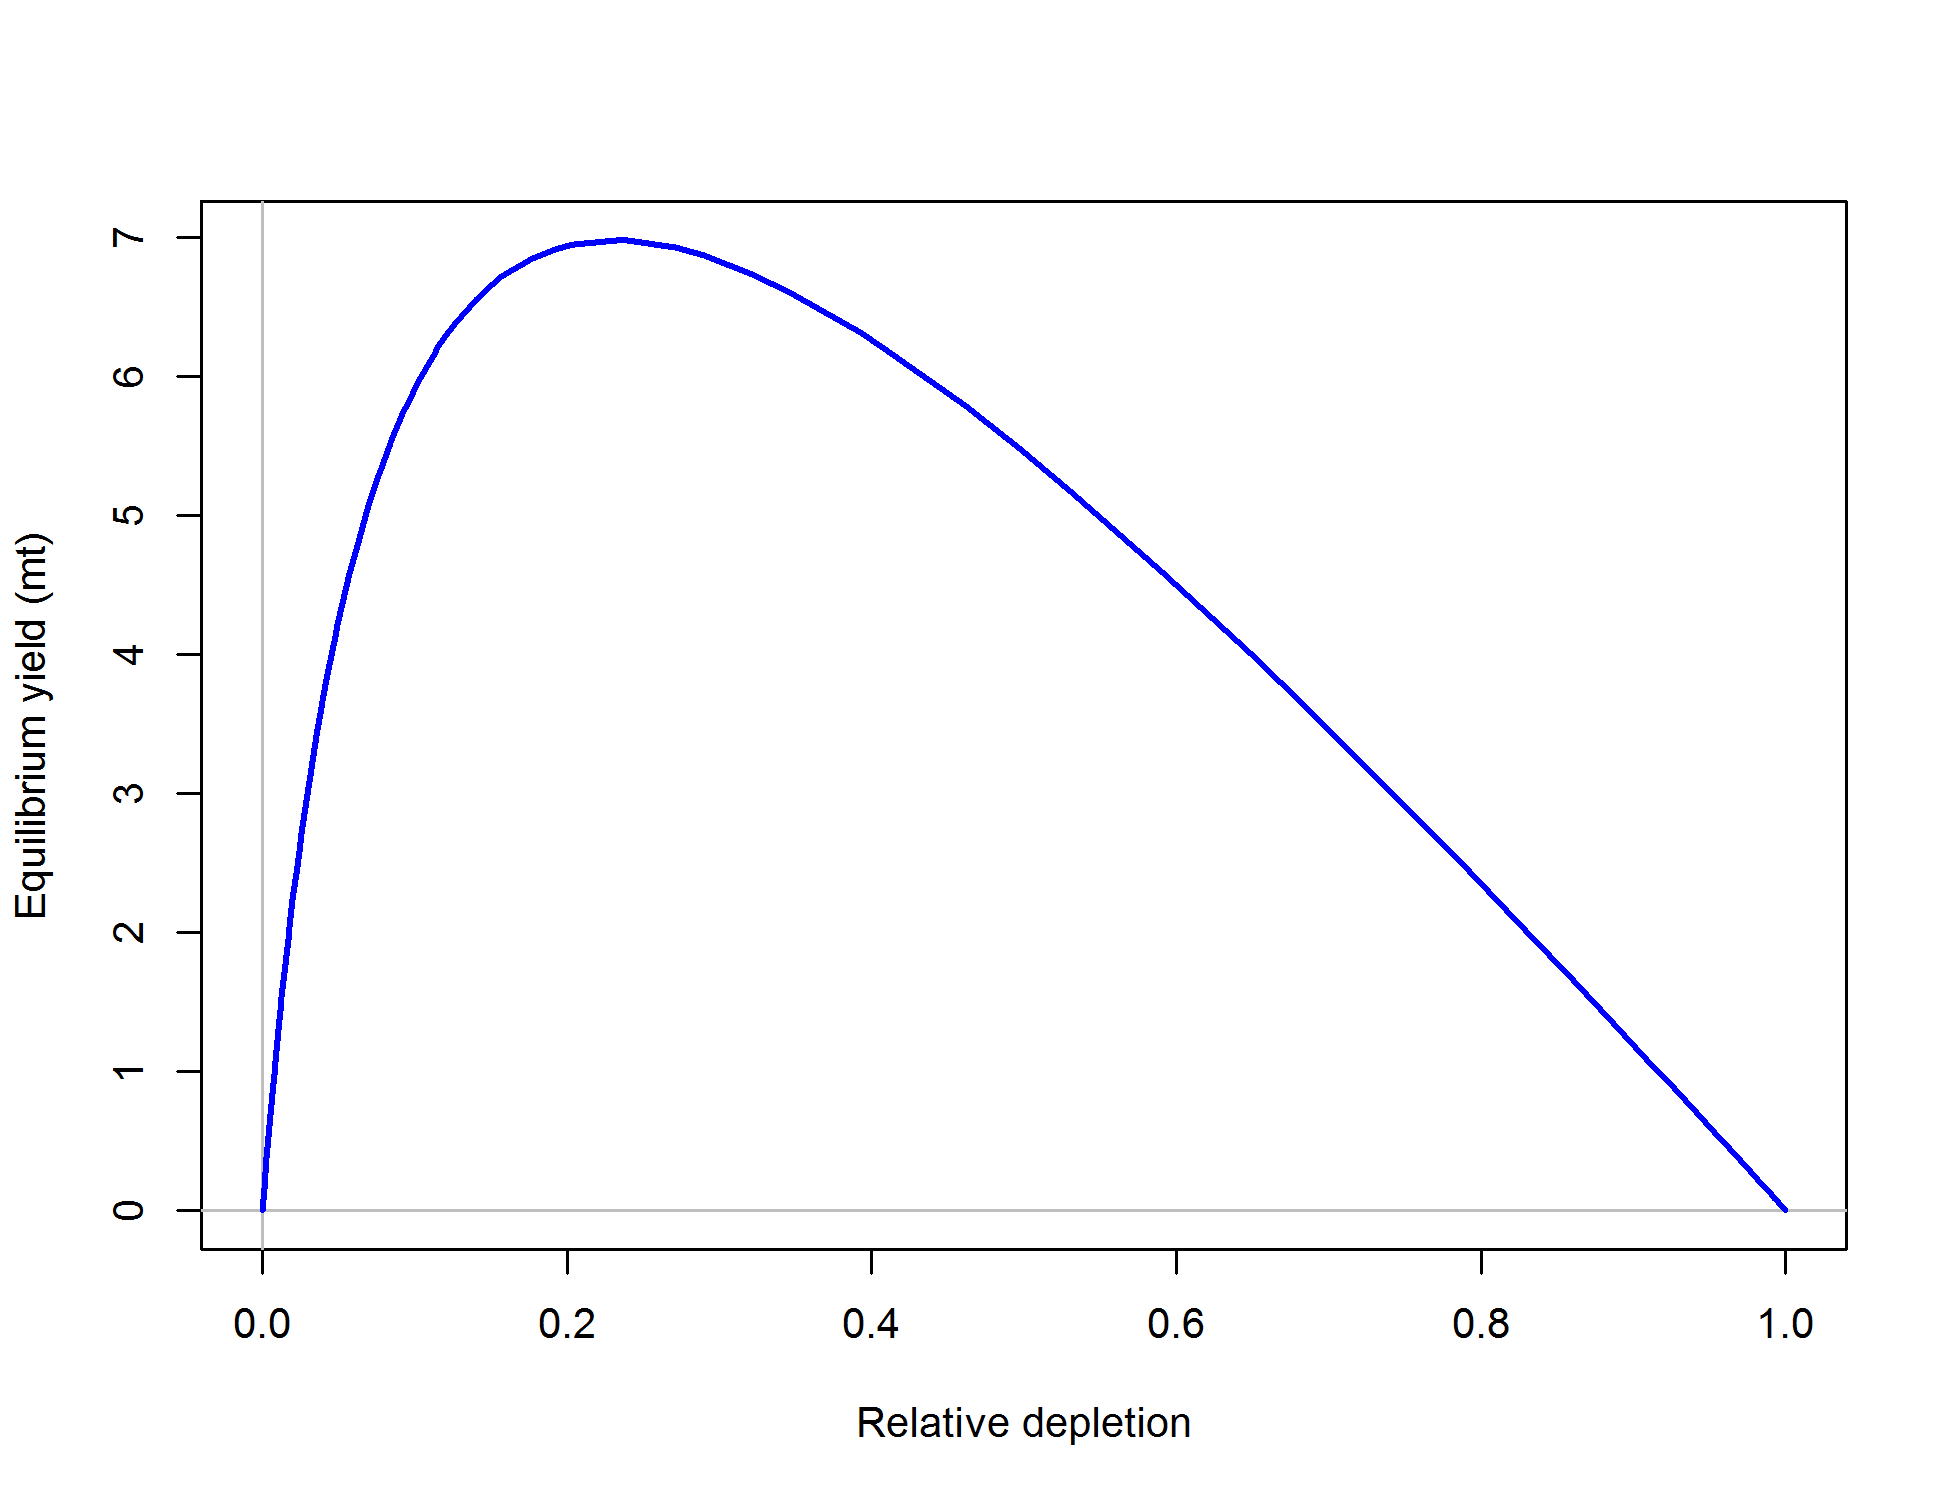
\includegraphics{r4ss/plots_mod1/yield1_yield_curve.png}
\caption{Equilibrium yield curve for the base case model. Values are
based on the 2016 fishery selectivity and with steepness fixed at 0.50.
\label{fig:Yield_all}}
\end{figure}

\FloatBarrier

\newpage

\renewcommand{\thefigure}{\arabic{figure}}
\renewcommand{\thetable}{\arabic{table}}

\setcounter{figure}{0} \setcounter{table}{0}

\pagenumbering{arabic}

\section{Introduction}\label{introduction}

\subsection{Basic Information}\label{basic-information}

Pacific ocean perch (\emph{Sebastes alutus}) are most abundant in the
Gulf of Alaska, and have been observed off of Japan, in the Bering Sea,
and south to Baja California, although they are sparse south of Oregon
and rare in southern California. While genetic studies have found three
populations of Pacific ocean perch off of British Columbia (Seeb and
Gunderson \protect\hyperlink{ref-seeb_genetic_1988}{1988}, Withler et
al. \protect\hyperlink{ref-withler_co-existing_2001}{2001}) with,
notably, a separate stock off of Vancouver Island, no significant
genetic differences have been found in the range covered by this
assessment. Pacific ocean perch show dimorphic growth, with females
reaching a slightly large size than males. Males and females are equally
abundant on rearing grounds at age 1.5.

The Pacific ocean perch population has been modeled as a single stock
off of the US West Coast (essentially northern California to the
Canadian border, since Pacific ocean perch are seen extremely rarely in
central and southern California). Good recruitments show up in
size-composition data throughout all portions of this area, which
supports the single stock hypothesis. This assessment includes landings
and catch data for Pacific ocean perch from the states of Washington,
Oregon and California, along with records from foreign fisheries, the
at-sea hake fleet, and fishery-indepenent surveys.

Prior to 1966, the Pacific ocean perch resource off of the northern
portion of the US West Coast was harvested almost entirely by Canadian
and United States vessels. Harvest was negligible prior to 1940, reached
1,300 mt in 1950, 3,200 mt in 1961 and exceeded 7,600 mt in 1965.
Catches increased dramatically after 1965, with the introduction of
large distant-water fishing fleets from the Soviet Union and Japan. Both
nations employed large factory stern trawlers as their primary method
for harvesting Pacific ocean perch. Peak removals by all foreign nations
combined are estimated at over 15,000 mt in 1966 and remained over
12,000 mt in 1967. These numbers are based upon a re-analysis of the
foreign catch data (Rogers
\protect\hyperlink{ref-rogers_species_2003}{2003}), which focused on
deriving a more realistic species composition for catches previously
identified only as Pacific ocean perch. Catches declined rapidly
following these peak years, and Pacific ocean perch stocks were
considered to be severely depleted throughout the Oregon-Vancouver
Island region by 1969 (Gunderson
\protect\hyperlink{ref-gunderson_population_1977}{1977}, Gunderson et
al. \protect\hyperlink{ref-gunderson_status_1977}{1977}). Landed harvest
averaged 1,350 mt over the period 1977-94. Landings have continued to
decline since 1994, primarily due to more restrictive management (Table
\ref{tab:Comm_Catch} and Figure \ref{fig:Catch}).

Prior to 1977, Pacific ocean perch in the northeast Pacific were managed
by the Canadian Government in its waters and by the individual states in
waters off of the United States. With implementation of the Magnuson
Fishery Conservation and Management Act (MFCMA) in 1977, US territorial
waters were extended to 200 miles from shore, and primary responsibility
for management of the groundfish stocks off Washington, Oregon and
California shifted from the states to the Pacific Fishery Management
Council (PFMC) and the National Marine Fisheries Service (NMFS). At that
time, however, a Fishery Management Plan (FMP) for the West Coast
groundfish stocks had not yet been approved. In the interim, the state
agencies worked with the PFMC to address conservation issues. In 1981,
the PFMC adopted a management strategy to rebuild the depleted Pacific
ocean perch stocks to levels that would produce Maximum Sustainable
Yield (MSY) within 20 years. On the basis of cohort analysis (Gunderson
\protect\hyperlink{ref-gunderson_results_1978}{1978}), the PFMC set
Acceptable Biological Catch (ABC) levels at 600 mt for the US portion of
the Vancouver INPFC area and 950 mt for the Columbia INPFC area. To
implement this strategy, the states of Oregon and Washington each
established landing limits for Pacific ocean perch. Trawl trip limits of
various forms remained in effect through 2016 (Table \ref{tab:Regs}).

Age estimates for Pacific ocean perch prior to the 1980s were made via
surface ageing of otoliths, which misses the very tight annuli at the
edge of the otolith once the fish reaches near maximum size. Ages are
biased by around age 10-12, and maximum age was estimated to be in the
20s, which lead to an overestimate of the natural mortality rate and the
productivity of the stock. Using break and burn methods, Pacific ocean
perch have been aged to over 100 years, and we now know that the
underlying assumptions of the early models were overly optimistic about
productivity. Research surveys have been used to provide
fishery-independent information about the abundance, distribution, and
biological characteristics of Pacific ocean perch. A coast-wide survey
of the rockfish resource was conducted in 1977 (Gunderson and Sample
\protect\hyperlink{ref-gunderson_distribution_1980}{1980}) and was
repeated every three years through 2004 (referred to as the `Triennial
Survey'). The National Marine Fisheries Service (NMFS) coordinated a
cooperative research survey of the Pacific ocean perch stocks off
Washington and Oregon with the Washington Department of Fisheries (WDFW)
and the Oregon Department of Fish and Wildlife (ODFW) in March-May 1979
(Wilkins and Golden
\protect\hyperlink{ref-wilkins_condition_1983}{1983}). This survey was
repeated in 1985 (referred to as the Pacific ocean perch Survey). Two
slope surveys have been conducted off the West Coast in recent years,
one using the research vessel Miller Freeman, which ended in 2001
(referred to as the `AFSC Slope Survey'), and another ongoing
cooperative survey using commercial fishing vessels which began in 1998
as a DTS (Dover sole, thornyhead and sablefish) survey, was expanded to
other groundfish in 1999 (referred to as the `NWFSC Slope Survey'). In
2003, this survey was expanded spatially to include the shelf. This last
survey, conducted by the NWFSC, continues to cover depths from 30-700
fathoms (55-1280 meters) on an annual basis (referred to as the `NWFSC
Shelf-Slope Survey').

\subsection{Summary of Management
History}\label{summary-of-management-history}

The landings of Pacific ocean perch have been historically governed by
harvest guidelines and trip limits, while recently management is imposed
with total catch harvest limits in the form of overfishing limits
(OFLs), acceptable biological catches (ABCs), and annual catch limits
(ACLs). A trawl rationalization program, consisting of an individual
fishing quota (IFQ) or catch shares system was implemented in 2011 for
the limited entry trawl fleet targeting non-whiting groundfish,
including Pacific ocean perch, and the trawl fleet targeting and
delivering whiting to shore-based processors. The limited entry at-sea
trawl sectors (motherships and catch-processors) that target whiting and
process at sea are managed in a system of harvest cooperatives.

Limits onPacific ocean perch were first established in 1983 (Table
\ref{tab:mnmgt_perform_tables}). These were implemented as area
closures, trip limits, and cumulative landing limits. In 1999, Pacific
ocean perch was declared overfished with the assessment estimating the
spawning output below the management limit (25\% of virgin biomass). In
reaction to the overfished decleration, harvest limits were reduced
relative to previous years and a rebuilding plan was implemented in
2001.

\subsection{Fisheries off Canada and
Alaska}\label{fisheries-off-canada-and-alaska}

Pacific ocean perch can be found in waters off the US west coast and
northward through Alaskan waters. In contrast the Pacific ocean perch
stock off the US west coast, each assessed portion of the stock in
Canada and Alaskan waters are estimated to be above management targets.
The subset of the stock off the US west coast represents the tail of the
species distribution with little to no Pacific ocean perch being
encountered south of northern California. Pacific ocean perch are
harvested both in Canada and Alaska. The most recent updated assessments
for the Bering Sea and the Gulf of Alaska stocks determined that neither
stock are in an overfished state and recommended and acceptable
biological catch of 43,723 mt and 23,918 mt, respectively, for 2017.

In Canadian waters Pacific ocean perch has the largest single-species
quota, accounting for approximately 25\% of all rockfish landings by
weight in the bottom trawl fleet. The Canadian Pacific ocean perch stock
is broken into three seperate areas that are individually assessed. The
status of the stock within each area are above Canadian management
targets.

\section{Data}\label{data}

Data used in the Pacific ocean perch assessment are summarized in Figure
\ref{fig:data_plot}. A description of each data source is provided
below.

\subsection{Fishery-Independent Data:}\label{fishery-independent-data}

\subsubsection{Northwest Fisheries Science Center (NWFSC) shelf-slope
survey}\label{northwest-fisheries-science-center-nwfsc-shelf-slope-survey}

The NWFSC shelf-slope survey is based on a random-grid design; covering
the coastal waters from a depth of 55 m to 1,280 m (Bradburn et al.
\protect\hyperlink{ref-bradburn_2003_2011}{2011}). This design uses four
chartered industry vessels in most years, assigned to a roughly equal
number of randomly selected grid cells. The survey, which has been
conducted from late-May to early-October each year, is divided into two
2-vessel passes of the coast, which are executed from north to south.
This design therefore incorporates both vessel-to-vessel differences in
catchability as well as variance associated with selecting a relatively
small number (approximately 700) of cells from a very large population
of possible cells (greater than 11,000) distributed from the Mexican to
the Canadian border.

The data from the NWFSC shelf-slope survey was analyzed using a
spatio-temporal delta-model (Thorson et al.
\protect\hyperlink{ref-thorson_geostatistical_2015}{2015}), implemented
as an R package VAST (Thorson and Barnett
\protect\hyperlink{ref-thorson_comparing_2017}{2017}) and publicly
available online (\url{https://github.com/James-Thorson/VAST}). Spatial
and spatio-temporal variation is specifically included in both encounter
probability and positive catch rates, a logit-link for encounter
probability, and a log-link for positive catch rates. Vessel-year
effects were included for each unique combination of vessel and year in
the database, to account for the random selection of commercial vessels
used during sampling (Helser et al.
\protect\hyperlink{ref-helser_generalized_2004}{2004}, Thorson and Ward
(\protect\hyperlink{ref-thorson_accounting_2014}{2014})). Spatial
variation was approximated using 1000 knots, and use the bias-correction
algorithm (Thorson and Kristensen
\protect\hyperlink{ref-thorson_implementing_2016}{2016}) in Template
Model Builder (Kristensen et al.
\protect\hyperlink{ref-kristensen_tmb:_2016}{2016}). Further details
regarding model structure are available in the user manual
(\url{https://github.com/James-Thorson/VAST/blob/master/examples/VAST_user_manual.pdf}).

The smallest Pacific ocean perch tend to occur in the shallower depths
(\textless{} 200 m) with only larger individuals occurring at depths
deeper than 300 m. Data collected by the NWFSC Shelf-Slope survey
between depths of 55 - 549 m and north of \(42^\circ\) and south of
\(49^\circ\) were stratified to generate an index of abundance from
2003-2016. The estimated index of abundance is shown in Table
\ref{tab:Index_Summary}. The lognormal distribution with random
strata-year and vessel effects had the lowest AIC and was chosen as the
final model. The Q-Q plot does not show any departures from the assumed
distribution (Figure \ref{fig:nw_qq}). The indices for the NWFSC
shelf-slope survey show a tentative decline in the population between
2003 and 2009, with an increasing trend in biomass between the 2009 and
2016 median point estimates.

Length, age, and conditional age-at-length compositions were expanded
based upon the stratification. The number of tows with length data
ranged from 33 in 2006 to 69 in 2015 (Table \ref{tab:NWcombo_Lengths})
where ages were collected for Pacific ocean perch in nearly every tow
(Table \ref{tab:NWcombo_Ages}). The expanded length frequencies from
this survey show an increase in small fish starting in 2010 (Figure
\ref{fig:nw_Length}). The age frequencies provide clear evidence of
large year-classes moving through the population from the 1999, 2000,
and 2008 recruitment; with early indications of a large 2013 recruitment
(Figure \ref{fig:nw_Age}).

The effective sample sizes for length and marginal age composition data
for all fishery-independet surveys were calculated according to Stewart
\& Hamel (\protect\hyperlink{ref-stewart_bootstrapping_2014}{2014})
which determined that the approximate realized sample size for
shelf/slope rockfish species was 2.43*\(N_{\text{tow}}\). The effective
sample size of conditional-age-at-length data was set at the number of
fish at each length by year.

\subsubsection{Northwest Fisheries Science Center (NWFSC) slope
survey}\label{northwest-fisheries-science-center-nwfsc-slope-survey}

The NWFSC slope survey covered waters throughout the summer from 183 m
to 1280 m north of \(34^\circ 30^\prime\) S, which is near Point
Conception between 1999 and 2002. Tows conducted between the depths of
183 and 549 m were used to create an index of abundance using a bayesian
delta-GLMM and the VAST delta-GLMM models. The estimated index of
abundance is show in Table \ref{tab:Index_Summary}. Based on the
diagnostics the bayesian delta-GLMM, which does not account for spatial
effects, gamma distribution with year-vessel random effects was selected
as the final model. The Q-Q plot does not show any departures from the
assumed distribution (Figure \ref{fig:nw_slope_qq}). The trend of
abundance across the four surveys years was generally flat with high
estimated annual variance.

Length and age compositions were available for 2001 and 2002 and were
expanded based upon the survey stratification (Tables
\ref{tab:NWslope_Lengths} and \ref{tab:NWslope_Ages}. The expanded
length frequencies from this survey shows that primarily only large fish
were captured both years (Figure \ref{fig:nw_slope_Length}). The
majority of fish observed by this survey were aged at greater than 10
years (Figure \ref{fig:nw_slope_Age}).

\subsubsection{Alaska Fisheries Science Center (AFSC) slope
survey}\label{alaska-fisheries-science-center-afsc-slope-survey}

The AFSC slope survey operated during autumn (October-November) aboard
the R/V Miller Freeman. Partial survey coverage of the U.S. west coast
occurred during 1988-96 and complete coverage (north of
\(34^\circ 30^\prime\) S) during 1997, 1999, 2000, and 2001. Only the
four years of consistent and complete surveys plus 1996, which surveyed
north of \(43^\circ\) N latitude to the U.S.-Canada border, were used in
this assessment. The number of tows with length data ranged from 19 in
2000 to 48 in 1996 (Table \ref{tab:AFSC_Lengths}). Because a large
number of positive tows occurred in 1996, it was decided to include that
year, which surveyed from \(43^\circ\) N latitude to the U.S.-Canada
border. Therefore, only tows from \(43^\circ\) N latitude to the
U.S.-Canada border were used.

An index of abundance was estimated based on the data using the VAST
delta-GLMM model. The estimated index of abundance is shown in Table
\ref{tab:Index_Summary}. The lognormal distribution with random
strata-year had the lowest AIC and was chosen as the final model. The
Q-Q plot does not show any departures from the assumed distribution
(Figure \ref{fig:afsc_qq}). The trend in the indices was generally flat
over time.

Length compositions were available for each year the survey was
conducted. No age data were available from this survey. The expanded
length frequencies from this survey were generally of larger fish (
\textgreater{} 30 cm), expect for 1997 where the highest frequency of
fish were between 20 and 30 cm for both females and males (Figure
\ref{fig:afsc_Length}).

\subsubsection{Triennial Bottom Trawl
Survey}\label{triennial-bottom-trawl-survey}

The triennial survey was first conducted by the AFSC in 1977 and spanned
the time-frame from 1977-2004. The survey's design and sampling methods
are most recently described in (Weinberg et al.
\protect\hyperlink{ref-weinberg_estimation_2002}{2002}). Its basic
design was a series of equally-spaced transects from which searches for
tows in a specific depth range were initiated. The survey design has
changed slightly over the period of time. In general, all of the surveys
were conducted in the mid-summer through early fall: the 1977 survey was
conducted from early July through late September; the surveys from 1980
through 1989 ran from mid-July to late September; the 1992 survey
spanned from mid-July through early October; the 1995 survey was
conducted from early June to late August; the 1998 survey ran from early
June through early August; and the 2001 and 2004 surveys were conducted
in May-July.

Haul depths ranged from 91-457 m during the 1977 survey with no hauls
shallower than 91 m. The surveys in 1980, 1983, and 1986 covered the
West Coast south to \(36.8^\circ\) N latitude and a depth range of
55-366 meters. The surveys in 1989 and 1992 covered the same depth range
but extended the southern range to \(34.5^\circ\) N (near Point
Conception). From 1995 through 2004, the surveys covered the depth range
55-500 meters and surveyed south to \(34.5^\circ\) N. In the final year
of the triennial series (2004), the NWFSC's Fishery Resource and
Monitoring division (FRAM) conducted the survey and followed very
similar protocols as the AFSC.

Given the different depths surveyed during 1977, the data from that year
were not included in this assessment. Water hauls (Zimmermann et al.
\protect\hyperlink{ref-zimmermann_influence_2003}{2003}) and tows
located in Canadian waters were also excluded from the analysis of this
survey. The data was examined for varying distribution of length and/or
ages of fish based upon the shift in survey timing and little evidence
was found of ontogenetic shifts in Pacific ocean perch during the summer
months.Pacific ocean perch are rarely encountered south of \(40^circ\)
where the change in southern range of the survey would have no impact on
data collected regarding Pacific ocean perch. Given these factors the
Triennial survey was analyzed as a single time-series a departure from
how the previous assessment which split the time-series into and an
early (1980-1992) and a late period (1995-2004).

An index of abundance was estimated based on the data using the VAST
delta-GLMM model. The estimated index of abundance is shown in Table
\ref{tab:Index_Summary}. The lognormal distribution with random
strata-year had the lowest AIC and was chosen as the final model. The
Q-Q plot does not show any departures from the assumed distribution
(Figure \ref{fig:tri_qq}). The index shows a decline in abundance in the
early years of the time-series and abundance remaining flat for the
latter years.

Length and age compositions were expanded based upon the stratification.
The number of tows with length data ranged from 17 in 1986 to 81 in 1998
\ref{tab:TriennialLengths}. Ages were read using surface reading methods
until 1989 when the break-and-burn method replaced surface reads as the
best method to age Pacific ocean perch. Unfortunately, surface reading
of Pacific ocean perch otoliths results in significant underestimates of
age. Due to this, these otolith were excluded from analysis. The
available ages from the Triennial survey and the number of tows where
otoliths were collected are shown in Table \ref{tab:Triennial_Ages}. The
expanded length frequencies from this survey show an increase in small
fish starting in 1995 (Figure \ref{fig:Tri_Length}). The age frequencies
provide clear evidence of large year-classes moving through the
population from the 1999 and 2000 recruitment (Figure
\ref{fig:Tri_Age}).

\subsubsection{Pacific ocean perch
Survey}\label{pacific-ocean-perch-survey}

A survey targeted designed to sample Pacific ocean perch was conducted
in 1979 and again in 1985 (for a detailed description see (Ianelli et
al. \protect\hyperlink{ref-ianelli_status_1992}{1992}). An index of
abundance was estimated based on the data using the VAST delta-GLMM
model. The estimated index of abundance is shown in Table
\ref{tab:Index_Summary}. The lognormal distribution with random
strata-year had the lowest AIC and was chosen as the final model. The
Q-Q plot does not show any departures from the assumed distribution
(Figure \ref{fig:pop_qq}). The index shows a clear decline in abundance
between the two survey years.

Length and age compositions were expanded based on the stratification.
The survey had 125 and 126 Pacific ocean perch tows (Table
\ref{tab:POP_Lengths}) and ages were only available in 1985 due to
surface reads for the 1979 data (Table \ref{tab:POP_Ages}). The length
frequencies for both years are highest between the 30-45 cm range
(Figure \ref{fig:POP_Length}) with ages in 1985 having a large number of
fish age 40 and greater (Figure \ref{fig:POP_Age}).

\subsection{Fishery-Dependent Data}\label{fishery-dependent-data}

\subsubsection{Commercial Fishery
Landings}\label{commercial-fishery-landings}

\textbf{Washington}

Historical commercial fishery landings of Pacific ocean perch from
Washington for the years 1918-2016 were obtained from Theresa Tsou
(WDFW) and Phillip Weyland (WDFW). This assessment is the first Pacific
ocean perch assessment to include a state provide historical catch
reconstruction and hence, the historical catches for Washington vary
markedly from those used in the 2011 assessment. Due to Recent landings
(1981-2016) were obtained directly from Washington state rather than
from PacFIN (Pacific Fisheries Information Network (PacFIN) due to
identified missing catches not available within PacFIN for Pacific ocean
perch.

\textbf{Oregon}

Historical commercial fishery landings of Pacific ocean perch from
Oregon for the years 1892-1986 were obtained from Alison Dauble (ODFW).
A description of the methods can be found in Karnowski et al.
(\protect\hyperlink{ref-karnowski_historical_2014}{2014}). Recent
landings (1987-2016) were obtained from PacFIN retrieval dated May 2,
2017\}, Pacific States Marine Fisheries Commission, Portland, Oregon;
www.psmfc.org). The catch data in from the POP and POP2 categories
contained within PacFIN for Pacific ocean perch were used for this
assessment. Additional catches from 1987-1999 for Pacific ocean perch
under the UROCK category not yet available in PacFIN were received
directly from the state and combined with the catch data available for
that period within PacFIN.

\textbf{California}

Historical commercial fishery landings of Pacific ocean perch were
obtained directly from John Field at the SWFSC due to database issues
for the historical period for the California Cooperative Groundfish
Survey, also known as CALCOM (128.114.3.187) for the years 1916-1980. A
description of the methods can be found in (Ralston et al.
\protect\hyperlink{ref-ralston_documentation_2010}{2010}). Recent
landings (1981-2016) were obtained from PacFIN (Pacific Fisheries
Information Network (PacFIN) retrieval dated May 2, 2017, Pacific States
Marine Fisheries Commission, Portland, Oregon; www.psmfc.org).

\textbf{At-Sea Hake Fishery}

Catches of Pacific ocean perch are monitored aboard the vessel by
observers in the At-Sea hake Observer program (ASHOP) and were available
for the years of 1975-2016. Observers use a spatial sample design, based
on weight, to randomly choose a portion of the haul to sample for
species composition. For the last decade, this is typically 30-50\% of
the total weight. The total weight of the sample is determined by all
catch passing over a flow scale. All species other than hake are removed
and weighed, by species, on a motion compensated flatbed scale.
Observers record the weights of all non-hake species. Non-hake species
total weights are expanded in the database by using the proportion of
the haul sampled to the total weight of the haul. The catches of
non-hake species in unsampled hauls is determined using bycatch rates
determined from sampled hauls. Since 2001, more than 97\% of the hauls
have been observed and sampled.

\textbf{Foreign Catches}

From the 1960s through the early 1970s, foreign trawling enterprises
harvested considerable amounts of rockfish off Washington and Oregon,
and along with the domestic trawling fleet, landed large quantities of
Pacific ocean perch. Foreign catches of individual species were
estimated by Rogers (\protect\hyperlink{ref-rogers_species_2003}{2003})
and attributed to INPFC areas for the years of 1966-1976 for Pacific
ocean perch. The foreign catches were combined across areas for a
coastwide removal total.

\subsubsection{Discards}\label{discards}

Data on discards of Pacific ocean perch are available from two different
data sources. The earliest source is called the Pikitch data and comes
from a study organized by Ellen Pikitch that collected trawl discards
from 1985-1987 (Pikitch et al.
\protect\hyperlink{ref-pikitch_evaluation_1988}{1988}). The northern and
southern boundaries of the study were \(48^\circ 42^\prime\) N latitude
and \(42^\circ 60^\prime\) N. latitude respectively, which is primarily
within the Columbia INPFC area (Pikitch et al.
\protect\hyperlink{ref-pikitch_evaluation_1988}{1988} , Rogers and
Pikitch \protect\hyperlink{ref-rogers_numerical_1992}{1992}).
Participation in the study was voluntary and included vessels using
bottom, midwater, and shrimp trawl gears. Observers of normal fishing
operations on commercial vessels collected the data, estimated the total
weight of the catch by tow and recorded the weight of species retained
and discarded in the sample. Results of the Pikitch data were obtained
from John Wallace (pers comm, NWFSC, NOAA) in the form of ratios of
discard weight to retained weight of Pacific ocean perch and
sex-specific length frequencies. Discard estimates are shown in Table
\ref{tab:Discard}.

The second source is from the West Coast Groundfish Observer Program
(WCGOP). This program is part of the NWFSC and has been recording
discard observations since 2003. Table \ref{tab:Discard} shows the
discard ratios (discarded/(discarded + retained)) of Pacific ocean perch
from the WCGOP. Since 2011, when the trawl rationalization program was
implemented, observer coverage rates increased to nearly 100\% for all
the limited entry trawl vessels in the program and discard rates
declined compared to pre-2011 rates. Discard rates were obtained for
both the catch-share and the non-catch share sector for Pacific ocean
perch. A single discard rate was calculated by weighting discard rates
based on the commercial landings by each sector. Coeffienct of
variations were calculated by bootstrapping vessels within ports because
the observer program randomly chooses vessels within porats to be
observed in the non-catch shares sectors. Discard length composition for
the trawl fleet varied by year, with larger fish being discarded prior
to 2011 (Figure \ref{fig:WCGOP_discard}).

\subsubsection{Historical Commercial Catch-per-unit
effort}\label{historical-commercial-catch-per-unit-effort}

Data on catch-per-unit-effort (CPUE) in mt/hr from the domestic fishery
were combined for the INPFC Vancouver and Columbia areas (Table
\ref{tab:CPUE_Summary}, from Gunderson
(\protect\hyperlink{ref-gunderson_population_1977}{1977})). Although
these data reflect catch rates for the US fleet, the highest catch rates
coincided with the beginning of removals by the foreign fleet. This
suggest that, barring unaccounted changes in fishing efficiency during
this period, the level of abundance was high at that time. A CV of 0.40
was used in this assessment to be consistent with the CV observed in the
survey data.

\subsubsection{Fishery Length And Age
Data}\label{fishery-length-and-age-data}

Biological data from commercial fisheries that caught Pacific ocean
perch were extracted from PacFIN (PFSMFC) on May 4, 2017. Lengths taken
during port sampling in Oregon and Washington were used to calculate
length and age compositions. There were no biological data for Pacific
ocean perch available within PacFIN. The overwhelming majority of these
data were collected from the mid-water and bottom trawl gear, but
additional biological data were collected from non-trawl gear which was
grouped together with trawl gear data. Tables \ref{tab:Comm_Lengths} and
\ref{tab:Comm_Ages} show the number of trips and fish sampled, along
with the calculated sample sizes. Length and age data were acquired at
the trip level, and then aggregated to the state level. The sample sizes
were calculated via the Stewart Method (Ian Stewart, pers comm, IPHC)
which for commercial fishery data is:

\begin{centering}

Input effN = $N_{\text{trips}} + 0.138 * N_{\text{fish}}$ if $N_{\text{fish}}/N_{\text{trips}}$ is $<$ 44

Input effN = $7.06 * N_{\text{trips}}$ if $N_{\text{fish}}/N_{\text{trips}}$ is $\geq$ 44

\end{centering}

\subsection{Biological Data}\label{biological-data}

\subsubsection{Natural mortality}\label{natural-mortality}

Historic Pacific ocean perch ages determined using scales and surface
reading methods of otoliths, resulted in estimates of natural mortality
(\(M\)) of between 0.10 and 0.20yr\textsuperscript{-1} with a longevity
less than 30 years(Gunderson
\protect\hyperlink{ref-gunderson_population_1977}{1977}). Based on
break-and-burn method of age determination using otoliths, the maximum
age of Pacific ocean perch was revised to be 90 years (Chilton and
Beamish \protect\hyperlink{ref-chilton_age_1982}{1982}). The updated
understanding concerning Pacific ocean perch longevity reduced the
estimate of natural mortality based on Hoenig's
(\protect\hyperlink{ref-hoenig_empirical_1983}{1983}) relationship to
0.059yr\textsuperscript{-1}. The previous assessment applied a prior
distribution on natural mortality based upon multiple life history
correlates (including Hoenig's method, Gunderson gonadosomatic index
(\protect\hyperlink{ref-gunderson_trade-off_1997}{1997}), and McCoy and
Gillooly's (\protect\hyperlink{ref-mccoy_predicting_2008}{2008})
theoretical relationship) developed separately for female and male
Pacific ocean perch.

Hamel (\protect\hyperlink{ref-hamel_method_2015}{2015}) developed a
method for combining meta-analytic approaches to relating the natural
mortality rate M to other life-history parameters such as longevity,
size, growth rate and reproductive effort, to provide a prior on \(M\).
In that same issue of ICESJMS, Then et al.
(\protect\hyperlink{ref-then_evaluating_2015}{2015}), provided an
updated data set of estimates of \(M\) and related life history
parameters across a large number of fish species, from which to develop
an \(M\) estimator for fish species in general. They concluded by
recommending \(M\) estimates be based on maximum age alone, based on an
updated Hoenig non-linear least squares (nls) estimator
M=4.899A\_max\^{}(-.916). The approach of basing M priors on maximum age
alone was one that was already being used for West Coast rockfish
assessments. However, in fitting the alternative model forms relating
\(M\) to \(A_{\text{max}}\), Then et al.
(\protect\hyperlink{ref-then_evaluating_2015}{2015}) did not
consistently apply their transformation. In particular, in real space,
one would expect substantial heteroscedasticity in both the observation
and process error associated with the observed relationship of M to
\(A_{\text{max}}\). Therefore, it would be reasonable to fit all models
under a log transformation. This was not done. Revaluating the data used
in Then et al. (\protect\hyperlink{ref-then_evaluating_2015}{2015}) by
fitting the one-parameter \(A_{\text{max}}\) model under a log-log
transformation (such that the slope is forced to be -1 in the
transformed space (Hamel
\protect\hyperlink{ref-hamel_method_2015}{2015})), the point estimate
for \(M\) is:

\begin{centering}

$M=\frac{5.4}{A_{\text{max}}}$

\end{centering}

The above is also the median of the prior. The prior is defined as a
lognormal with mean \(ln(\frac{5.4}{A_{\text{max}}})\) and SE =
0.4384343. Using a maximum age of 100 the point estimate and median of
the prior is 0.054. The maximum age was selected based on available age
data from all West Coast data sources. The oldest aged rockfish was 120
years, captured by the commercial fishery in 2007. However, age data are
subject to ageing error which could impact this estimate of longevity.
The selection of 100 years was based on the range of other ages
available with had multiple observations of fish between 90 and 102
years of age.

\subsubsection{Sex ratio, maturation, and
fecundity}\label{sex-ratio-maturation-and-fecundity}

Examining all biological data sources, the sex ratio of young fish are
within 5\% of 1:1 by either length or age (Figures \ref{fig:sexratio}
and \ref{fig:sexratio_Age}), and hence this assessment the sex ratio at
birth was assumed to be 1:1. This assessment assumed a logistic
maturity-at-length curve based on analysis of 537 fish maturity samples
collected from the NWFSC shelf-slope survey. This is revised from the
previous assessment which assumed maturity-at-age based on the work of
Hannah and Parker (Hannah and Parker
\protect\hyperlink{ref-hannah_age-modulated_2007}{2007}). Additionally,
the new maturity-at-length curve is based on the estimate of functional
maturity an approach that classifies rockfish maturity with developing
oocytes as mature or immature based on the proportion of vitellogenin in
the cytoplasm and the measured frequency of atretic cells (M. Head, pers
comm, NWFSC, NOAA). The 50\% size-at-maturity was estimated at 32.1 cm
with maturity asymptoting to one for larger fish (Figure \ref{fig:mat}).
Comparison between the maturity-at-age used in the previous assessment
and the updated functional maturity-at-length is shown in Figure
\ref{fig:mat_compare}.

The fecundity-at-age has also been updated from the previous assessment
based on new research. Dick
(\protect\hyperlink{ref-dick_meta-analysis_2017}{2017}) estimated new
fecundity relationships for select West Coast stocks where fecundity for
Pacific ocean perch was estimated equal to
8.66e-10\(L\)\textsuperscript{4.98} in millions of eggs. Spawning output
at length is shown in Figure \ref{fig:fecundity}.

\subsubsection{Length-weight
relationship}\label{length-weight-relationship}

The length-weight relationship for Pacific ocean perch was estimated
outside the model using all biological data available from fishery and
fishery-independent data sources where the female weight-at-length in
grams was estimated at 1.044e-05\(L\)\textsuperscript{3.09} and males at
1.05e-05\(L\)\textsuperscript{3.08} where \(L\) is length in cm (Figures
\ref{fig:Wt_len} and \ref{fig:Wt_len_pred}).

\subsubsection{Growth (length-at-age)}\label{growth-length-at-age}

The length-at-age was estimated for male and female Pacific ocean perch
using data collected from both fishery-dependent and -independent data
sources that were collected from 1981-2016. Figure \ref{fig:Len_Age}
shows the lengths and ages for all years and all data as well as
predicted von Bertalanffy fits to the data. Females grow larger than
males and sex specific growth parameters were estimated at the following
values:

\begin{centering}

Females $L_{\infty}$ = 42.32; $k$ = 0.169; $t_0$ = -1.466

Males $L_{\infty}$ = 39.03; $k$ = 0.212; $t_0$ = -1.02

\end{centering}

\subsubsection{Ageing Precision And
Bias}\label{ageing-precision-and-bias}

Uncertainty surrounding the ageing-error process for Pacific ocean perch
was incorporated by estimating ageing error by age. Age-composition data
used in the model were from break-and-burn otolith reads aged by the
Cooperative Ageing Project (CAP) in Newport, Oregon. Break-and-burn
double reads of more than 1500 otoliths were provided by the CAP lab. An
ageing error estimate was made based on these double reads using a
computational tool specifically developed for estimating ageing error
(Punt et al. \protect\hyperlink{ref-punt_quantifying_2008}{2008}), and
using release 1.0.0 of the R package nwfscAgeingError (Thorson et al.
\protect\hyperlink{ref-thorson_nwfscageingerror:_2012}{2012}) for input
and output diagnostics, publicly available at:
\url{https://github.com/nwfsc-assess/nwfscAgeingError}. A non-linear
standard error was estimated by age where there is more variability in
the estimated age of older fish was estimated (Table
\ref{tab:Age_Error}, Figure \ref{fig:Age_Error}).

\subsection{History Of Modeling Approaches Used For This
Stock}\label{history-of-modeling-approaches-used-for-this-stock}

\subsubsection{Previous Assessments}\label{previous-assessments}

The status of Pacific ocean perch off British Columbia, Washington, and
Oregon have been periodically assessed since the intensive exploitation
that occured in the 1960s. Concerns regarding Pacific ocean perch status
off the coast the US west coast were raised in the late 1970s (Gunderson
\protect\hyperlink{ref-gunderson_results_1978}{1978}, Gunderson
(\protect\hyperlink{ref-gunderson_updated_1981}{1981})) and in 1981 the
PFMC adopted a 20-year plan to rebuild the stock.

The 1992 assessment determined that Pacific ocean perch remained at low
levels relative to the population size in 1960 (Ianelli et al.
\protect\hyperlink{ref-ianelli_status_1992}{1992}) and recommended
additional harvest restrictions to allow for stock rebuilding. The 1998
assessment (Ianelli and Zimmermann
\protect\hyperlink{ref-ianelli_status_1998}{1998}) estimated that the
stock was 13\% of the unfished level, leading the National Marine
Fishery Service (NMFS) to declare the stock overfished in 1999. The
formal rebuilding plan was implemented in 2001. The rebuilding plan
reduced the SPR harvest rate used to determine catches to 0.864,
relative to the PFMC rockfish default harvest (SPR = 0.50). The last
full assessment of Pacific ocean perch was conducted in 2011 (Hamel and
Ono \protect\hyperlink{ref-hamel_stock_2011}{2011}) which concluded that
the stock was still well below the target biomass of \(0.40SB_{0}\)
estimating the relative stock status at 19.1\%.

\subsubsection{Previous Assessment
Recommendations}\label{previous-assessment-recommendations}

Recommendation: Considering trans-boundary stock effects should be
pursued. In particular the consequences of having spawning contributions
from external stock components should be evaluated relative to the
steepness estimates obtained in the present assessment (see more
complete discussion of this recommendation under the Unresolved Problems
and Major Uncertainties section, above).

\emph{STAT response: The STAT team agrees that this should be an ongoing
area of research and collaboration between the US and Canada. This
assessment presents a sensitivity where the inclusion of Canadian data
are included within the model.}

Recommendation:The benefits of adopting the complex model used this year
should be evaluated relative to simpler assumptions and models. While
the transition from the simpler old model to Stock Synthesis was shown
to be similar for the historical period, the depletion estimates in the
most recent years were different enough to warrant further
investigation.

\emph{STAT response: This assessment was performed in Stock Synthesis,
an integrated model, which can be modified to either simple or complex
structural forms based upon the available data and the processes being
modeled. There were not addtional explorations of alternative modeling
platforms.}

Recommendation:Discard estimates from observer programs should be
presented, reviewed (similar to the catch reconstructions), and be made
available to the assessment process.

\emph{STAT response: This assessment uses discard rates and discard
lengths collected by the WCGOP from 2003-2015.}

Recommendation:The ability to allow different ``plus groups'' for
specific data types should be evaluated (and implemented in Stock
Synthesis). For example, this would provide the ability to use the
biased surface-aged data in an appropriate way.

\emph{STAT response: Additional research needs to completed which
evaluates the amount of bias and imprecision in surface-read ages.
Evaluating avaiable surface-read ages within the PacFIN database fish of
lengths between 23-44 cm can be aged at 10 years old. This large range
of lengths at the same age indicates considerable bias in ages for fish
surface-read younger aged fish.}

Recommendation:Historical catch reconstruction estimates should be
formally reviewed prior to being used in assessments and should be
coordinated so that interactions between stocks are appropriately
treated. The relative reliability of the catch estimates over time could
provide an axis of uncertainty in future assessments.

\emph{STAT response: California and Oregon have ungone extensive work to
create historical catch reconstructions. This is the first assessment
for Pacific ocean perch which includes a Washington historical catch
reconstruction. The data used in this assessment represent Washington
state's current best estimate for historical catches. Both California
and Washington are conducting research to estimate uncertainty surround
historical catches which could be used to propegate uncertainty within
the assessment.}

\section{Assessment}\label{assessment}

\subsection{General Model Specifications and
Assumptions}\label{general-model-specifications-and-assumptions}

Stock Synthesis v3.30.03.05 was used to estimate the parameters in the
model. R4SS, revision 1.27.0, along with R version 3.3.2 were used to
investigate and plot model fits. A summary of the data sources used in
the model (details discussed above) is shown in Figure
\ref{fig:data_plot}.

Stock Synthesis has many options when setting up a model and the
assessment model for Pacific ocean perch was set up in the following
manner.

\subsubsection{Changes between the 2011 assessment model and current
model}\label{changes-between-the-2011-assessment-model-and-current-model}

The current model for Pacific ocean perch has many made many similar
assumptions to the 2011 assessment but differs in some key ways. This
assessment disaggrated the fleets into a trawl/other gear, at-sea hake,
historical foreign fleet, and research fleets. The previous assessment
implemented a single fleet where removal from all sources were
aggregated together. The seperating of fleets applied in this assessment
allowed for differing assumptions regarding current and historical
discarding practices. Although there are no compositional data available
from the foreign fleet, it is assumed that very little discarding to no
discarding of fish occured. Additionally, the at-sea hake fishery
removals are represent both discarded and retained fish and hence an
additional discard rate would not be appropriate. Similar logic was
applied in regard to survey and research removals.

The historical landing used in the model differs from those used in
2011. The assessment includes the first state provided historical
reconstruction landings for Washington state. The historical
reconstruction provided Pacific ocean perch landing within Washington
state starting in 1916 and have larger removals in the 1940s relative to
those used in 2011 \ref{fig:Catch_Compare}. Given the increase in
historical removals prior to 1940, the 2011 model starting year, the
starting year for modeling the stock was revised to 1918, the first year
Pacific ocean perch landings exceeded 1 mt, for this assessment.
Explorations were conducted relative to the model starting year and no
differences were found between the 1918 start year compared to starting
the model in 1892, the first record of Pacific ocean perch landings
between California, Oregon, and Washington catch data.

Selectivity in this model is assumed to be length-based and is modeled
using double-normal for all fleets, expect the Pacific ocean perch
survey which retained the previous assessment assumption of logistic
selectivity. The previous assessment mirrored selectivity amont the
Pacific ocean perch and both slope surveys (AFSC and NWFSC). This
assessment allow for survey specific estimated double-normal
selectivity.

All fishery-independent indices have been reevaluated for this
assessment using a spatial-temporal delta generalized linear mixed model
(VAST delta-GLMM) which is updated from 2011 which used a bayesian
delta-GLMM which did not incorporate spatial effects. An additional
update to the treatment of survey data was the decision to use the
Triennial survey as a single time series ranging from 1980-2004. The
previous assessment opted to split this survey into early and a late
index of abundance based upon the change in southern sampling and a
shift in survey timing. Northern California is considered to be the
southern end of Pacific ocean perch West Coast distribution with rare
encounters in central or southern California waters. The biological data
from the Triennial survey showed no discernable ontogenetic shifts in
Pacific ocean perch during the early or late period of summer samples.
Based upon these investigations, the Triennial survey was retained as a
single index of abundance.

Maturity and fecundity were updated for this assessment based upon new
research. Fecundity for Pacific ocean perch used in this assessment was
base on reevaluation of the fecundity of West Coast rockfish by Dick et
al. (\protect\hyperlink{ref-dick_meta-analysis_2017}{2017}) updating the
previous fecundity estimates used in the 2011 assessment (Dick
\protect\hyperlink{ref-dick_modeling_2009}{2009}) (Figure
\ref{fig:fecundity}). Maturity in this assessment was based on
examination of 537 fish samples which were used to estimate functional
maturity, an approach that classifies rockfish maturity with developing
oocytes as mature or immature based on the proportion of vitellogenin in
the cytoplasm and the measured frequency of atretic cells (M. Head, pers
comm, NWFSC, NOAA). The updated maturity curve was based on
maturity-at-length where the previous estimates used in 2011 were based
on maturity-at-age (Figure \ref{fig:mat_compare}).

In this assessment, the beta prior developed from a meta-analysis of
West Coast groundfish was updated to the 2017 value (J. Thorson, pers
comm, NWFSC, NOAA) in preliminary models, with steepness fixed in the
final base model. Additionally, the prior for natural mortality was
updated base on analysis conducted by Owen Hamel (pers comm, NWFSC,
NOAA), where female natural mortality was fixed at the prior median with
males estimated as an offset from the female value.

\subsubsection{Summary of Fleets and
Areas}\label{summary-of-fleets-and-areas}

Pacific ocean perch are most frequently observed in Oregon and
Washington waters, however, they are observed along the entire US West
Coast in survey and fishery observations. Multiple fisheries encounter
Pacific ocean perch. Trawl, fixed gear, and the at-sea (mid-water) hake
fisheries account for the majority of the Pacific ocean perch landings
both historically and currently.

The majoirty of removals of Pacific ocean perch were observed by eht
bottom trawl fishery with fixed gear accounting for a small fraction of
the catches avaiable within PacFIN. Trawl and fixed gears were combined
into a coast-wide fleet. For the period from 1918 to the early 1990s,
prior to the introduction of trip limits for rockfish, limited
discarding of Pacific ocean perch was assumed. Observations of Pacific
ocean perch in the Pikitch et al. (1988) data (1986-1987) allowed for a
formal analysis of discard rates which were applied to the historical
period of the fishery. Foreign trawl catches (1966-1976) was modeled as
a single fleet. The at-sea fishery operates as a mid-water fishery
targeting Pacific whiting but encounters Pacific ocean perch as a
bycatch species. This fleet was also modeled as a single fleet.

\subsubsection{Other Specifications}\label{other-specifications}

The specifications of the assessment are listed in Table
\ref{tab:Model_setup}. The model is a two-sex, age-structured model
starting in 1918 with an accumulated age group at 60 years. Growth was
estimated and natural mortality was fixed at the median of the prior.
The lengths in the population were tracked by 1 cm intervals and the
length data were binned into 1 cm intervals. A curvilinear ageing
imprecision relationship was estimated and used to model ageing error.
Fecundity-at-length was defined fixed at the values from Dick et al.
(\protect\hyperlink{ref-dick_meta-analysis_2017}{2017}) for Pacific
ocean perch and spawning output was defined in millions of eggs.

The Triennial survey was kept as a single series. Assessment of other
groundfish have split this survey into an early and a late series, based
mostly on the shift to deeper depths and the timing of the survey, by
estimating different catchability parameters and selectivity parameters
for each period. Age data were available for the commercial and at-sea
hake fishery, as well as the Triennial, the Pacific ocean perch, the
NWFSC slope, and the NWFSC shelf-slope survies. The ages from the NWFSC
shelf-slope survey and were entered into the model as conditional
age-at-length. Length-frequencies were calculated for the Triennial,
Pacific ocean perch, AFSC slope, NWFSC slope, and the NWFSC shelf-slope
surveys within each stratum, and then combined across strata using the
biomass in each stratum as the weighting factor. This reduced the
influence of a few fish observed in a large area.

The specification of when to estimate recruitment deviations is an
assumption that likely affects model uncertainty. It was decided to
estimate recruitment deviations from 1900-2014 to appropriately quantify
uncertainty. The earliest length-composition data occur in 1966 and the
earliest age data were in 1981. The most informed years for estimating
recruitment deviations were from about the mid-1970s to about 2011. The
period from 1900-1974 was fit using an early series with little or no
bias adjustment, the main period of recruitment deviates occurred from
1975-2014 with an upward and downward ramping of bias adjustment, and
2015 onward was fit using forecast recruitment deviates with little bias
adjustment. Methot and Taylor
(\protect\hyperlink{ref-methot_adjusting_2011}{2011}) summarize the
reasoning behind varying levels of bias adjustment based on the
information available to estimate the deviates. Recruitment deviation
was assumed to be 0.70.

The recommended selectivity type in Stock Synthesis is the double normal
and was used in this assessment for the all fleets, except the Pacific
ocean perch survey which was assumed logistic based on the length
composition data. Changes in retention curves were estimated for the
commercial fishery.

Time blocks for the bottom trawl, midwater trawl, and hook-and-line
fishery are provided in Table \ref{tab:Model_setup}. Fishery selectivity
retention has changed over the modeled period due to management changes.
The time block on the retention curves for the trawl fishery were set
from 1918-1991, 1992-2001, 2002-2007, 2008, 2009-2010, 2011-2016 based
on available discarding data and changes in trip limits that likely
resulted in changes to discarding patterns of Pacific ocean perch. No
discarding was assumed in the at-sea hake and the foreign fisheries.

The following distributions were assumed for data fitting. Survey
indices were lognormal, total discards were lognormal.

\subsubsection{Modeling Software}\label{modeling-software}

The STAT team used Stock Synthesis version 3.30.03.05 by Dr.~Richard
Methot at the NWFSC (Methot and Wetzel
\protect\hyperlink{ref-methot_stock_2013}{2013}). This most recent
version was used, since it included improvements and corrections to
older versions. The previous assessment of Pacific ocean perch also used
Stock Synthesis but a earlier version, 3.24, model bridging was
performed between both version of Stock Synthesis and are shown in
Figure \ref{fig:bridge}.

\subsubsection{Priors}\label{priors}

A prior distribution was developed for the natural mortality parameter
from an analysis of a maximum age of 100 years. The analysis was
performed by Owen Hamel (pers comm, NWFSC, NOAA) and used data from Then
et al. (\protect\hyperlink{ref-then_evaluating_2015}{2015}) to provide a
lognormal distribution for natural mortality. The median of the
lognormal prior is 0.054 and has a standard error of 0.4384343.

The prior for steepness (\(h\)) assumes a beta distribution with
parameters based on an update of the Dorn rockfish prior (commonly used
in past West Coast rockfish assessments) conducted by J. Thorson (pers
comm, NWFSC, NOAA) which was reviewed and endorsed by the SSC in 2017.
The prior is a beta distribution with \(\mu\)=0.72 and \(\sigma\)=0.15.
However, fixing steepness within the model resulted in unrealistic
relative biomass levels (\(>\) 1), it was also decided to fix steepness
at 0.50. The previous assessment estimated and fixed steepness equal to
0.40. The current data does not contain information regarding steepness
and 0.50 was selected as an intermediate value between the prior and the
previous assessment value. The steepness value of 0.50 was contained
within the estimated uncertainty envelope from the assessment model when
either the prior value of 0.72 or 0.40 values were assumed.

\subsubsection{Data Weighting}\label{data-weighting}

The base case was weighted such that the various data sources were
mostly consistent with each other in terms of the relationship between
input and effective sample sizes. Length and age-at-length compositions
from the NWFSC shelf-slope survey were fit along with length and
marginal age compositions from the fishery fleets. Length data started
with a sample size determined from the equation listed in Section
\ref{fishery-length-and-age-data} and
\ref{northwest-fisheries-science-center-nwfsc-shelf-slope-survey}.
Age-at-length data assumed that each age was a random sample within the
length bin and started with a sample size equal to the number of fish in
that length bin. However, the 2016 NWFSC shelf-slope age-at-length data
was variable compared to previous years for both males and females
relative to all other years with observed fish being smaller at age. Due
to the increased variability within this data year, the effective sample
size for this year was reduced to 50\% of the number of fish within each
length-age bin.

One extra variability parameter that was added to the input variance was
estimated for the Triennial and the NWFSC shelf-slope survey indices.
Vessels present in the WCGOP data were bootstrapped to provide
uncertainty of the total discards (Table \ref{tab:Discard}).

The base case assessment model was weighted based on the ``Francis
method'', which was based on equation TA1.8 in Francis
(\protect\hyperlink{ref-francis_data_2011}{2011}). This formulation
looks at the mean length or age and the variance of the mean to
determine if across years, the variability is explained by the model. If
the variability around the mean does not encompass the model
predictions, then that data source should be down-weighted. This method
does account for correlation in the data (i.e., the multinomial
distribution) as opposed to the McAllister and Ianelli
(\protect\hyperlink{ref-mcallister_bayesian_1997}{1997}) method of
looking at the difference between individual observations and
predictions.

\subsubsection{Estimated And Fixed
Parameters}\label{estimated-and-fixed-parameters}

There were 164 estimated parameters in the base case model. These
included one parameter for \(R_0\), 8 parameters for growth, 2
parameters for extra variability on the Triennial and NWFSC shelf-slope
surveys indices, 24 parameters for selectivity, retention, and time
blocking of the fleets and the surveys, 117 recruitment deviations, and
12 forecast recruitment deviations (Table \ref{tab:model_params}).

Fixed parameters in the model were as follows. Steepness was fixed at
0.50. A sensitivity analysis and a likelihood profile were done for
steepness. Natural mortality was fixed at 0.054 for females and males,
which is the median of the prior. The standard deviation of recruitment
deviates was fixed at 0.70. Maturity at age was fixed as described in
Section \ref{sex-ratio-maturation-and-fecundity}. Length-weight
parameters were fixed at estimates using all length-weight observations
(Figure \ref{fig:Wt_len_pred}).

Dome-shaped selectivity was explored for both the fishery and the
surveys. Older Pacific ocean perch are often found in deeper waters and
may move into areas that limit their availability to fishing gear,
especially trawl gear. Domed shape selectivity was assumed for the
fishery fleet and the Triennial survey. The final base model assumed
asymptotic selectivity for the at-sea hake fishery, and all other
surveys.

\subsection{Model Selection and
Evaluation}\label{model-selection-and-evaluation}

The base case assessment model for Pacific ocean perch was developed to
balance parsimony and realism, and the goal was to estimate a biomass
trajectory for the population of Pacific ocean perch on the west coast
of the United States. The model contains many assumptions to achieve
parsimony and uses many different sources of data to estimate reality. A
series of investigative model runs were done to achieve the final base
case model.

\subsubsection{Key Assumptions and Structural
Choices}\label{key-assumptions-and-structural-choices}

The key assumptions in the model were that the assessed population is a
single stock with biological parameters characterizing the entire coast,
maturity at age has remained constant over the period modeled,
weight-at-length has remained constant over the period modeled, the
standard deviation in recruitment deviation is 0.70, and steepness is
0.50. These are simplifying assumptions that unfortunately cannot be
verified or disproven. Sensitivity analyses were conducted for most of
these assumptions to determine their effect on the results.

Structurally, the model assumed that the catches from each fleet were
representative of the coastwide population, instead of specific areas,
and fishing mortality prior to 1918 was negligible. It also assumed that
discards were low prior to 1992 and after 2010.

\subsubsection{Alternate Models
Considered}\label{alternate-models-considered}

The exploration of models began by bridging from the 2011 assessment to
SS version 3.24U, which produced no discernable difference. The updated
catch series with discards added per the 2011 assessment produced
insignificant differences in the relative scale of the population
although the updated historical removals resulted in an increase in the
estimate of unfished biomass. Updating the survey indices produced small
differences in the relative scale of the population. Adding age and
length data each resulted in less of a population decline from the 1970s
to pre-2000, resulting in an increase in the estimated final stock
status as of 2017. However, the addition of new data resulted in an
early pattern within recruitment, indicating that the assumptions within
the previous model may not represent the best fit to the current data.

This assessment estimated discards in the model, so time was spent
investigating time blocks for changes in selectivity and retention to
match the limited discard data as best as possible. Using major changes
in management and observed changes in landings, a set of blocks for
retention was found for the bottom trawl fleets. In the spirit of
parsimony, we used as few blocks as possible, allowed blocks only for
time periods with data, and added new blocks when we felt they were
justified by changes in management and they improved the fit to the
data.

Natural mortality was also investigated and a new prior was developed
assuming a maximum age of 100 years for females and males. The previous
assessment estimated male natural mortality as an offset from female
natural mortality which was fixed at the median of the 2011 prior. This
assessment attempted to estimate natural mortality for both sexes using
the 2017 updated prior, but there was little to no information on
natural mortality within the data and hence opted to fix the value for
females. Upon additional exploration, the model estimated very little
difference in male natural mortality relative to females (\textless{}
0.002) and in the interest of selecting the model that fit the data with
the fewest parameters required, males were fixed equal to the female
natural mortality.

Finally, multiple models were investigated where steepness either
estimated, fixed at the prior, or at an alternate value. The assessment
in 2011 determined that there was sufficient information concerning
steepness where the parameter was estimated and then fixed at 0.40.
Based upon likelihood profiles performed on the current assessment,
there was no longer support for a steepness value of 0.40 and the
likelihood profile was flat across various levels of steepness with a
very small improvement in likelihood (\textless{}0.50 log likelihood
units) at the lowest steepness values. Estimating steepness starting at
the median of the ``type C'' prior, the meta-analysis prior evaluated
omitting information from Pacific ocean perch, of 0.76 resulted in very
little if any movement from the median value due to the flat likelihood
surface across values for this parameter with final relative stock
status for 2017 being estimated to \textgreater{} 100\% of unfished
biomass. Fixing steepness at the median of the prior of 0.72 resulted in
relative stock status estimates for 2017 at 98.6\% of unfished biomass.
It was determined that the resulting stock status estimates when
steepness was fixed at the meta-analysis prior were overly optomistic
and unrealistic given the biology and historical exploitation of Pacific
ocean perch.

\subsubsection{Convergence}\label{convergence}

Proper convergence was determined by starting the minimization process
from dispersed values of the maximum likelihood estimates to determine
if the model found a better minimum. This was repeated 100 times and a
better minimum was not found (Table \ref{tab:jitter}). The model did not
experience convergence issues when provided reasonable starting values.
Through the jittering done as explained above and likelihood profiles,
we are confident that the base case as presented represents the best fit
to the data given the assumptions made. There were no difficulties in
inverting the Hessian to obtain estimates of variability, although much
of the early model investigation was done without attempting to estimate
a Hessian.

\subsection{Response To The Current STAR Panel
Requests}\label{response-to-the-current-star-panel-requests}

\begin{description}[style=unboxed]

\item[Request No. 1: Add after STAR panel.] \hfill \\

    \textbf{Rationale:} Add after STAR panel.  

    \textbf{STAT Response:} Add after STAR panel.

\item[Request No. 2: Add after STAR panel.] \hfill \\

    \textbf{Rationale:} Add after STAR panel.

    \textbf{STAT Response:} Add after STAR panel.

\item[Request No. 3: Add after STAR panel.] \hfill \\

    \textbf{Rationale:} Add after STAR panel.
  
    \textbf{STAT Response:} Add after STAR panel.

\item[Request No. 4: Example of a request that may have a list:] \hfill \\
\begin{itemize}
\item \textbf{Item No. 1}
\item \textbf{Item No. 2}
\item \textbf{Item No. 3, etc.}
\end{itemize}

\end{description}

\subsection{Base Model Results}\label{base-model-results}

The base model parameter estimates along with approximate asymptotic
standard errors are shown in Table \ref{tab:model_params} and the
likelihood components are shown in Table \ref{tab:like}. Time-series of
estimated stock size over time are shown in Table
\ref{tab:Timeseries_mod1}. Estimates of key derived parameters and
approximate 95\% asymptotic confidence intervals are shown in Table
\ref{tab:Ref_pts}.

\subsubsection{Parameter Estimates}\label{parameter-estimates}

The estimates of maximum length and the von Bertanlaffy growth
coefficient, \(k\), were less than the the external estimates for males
and females (Figure \ref{fig:Len_Age}, but were well within the 95\%
confidence interval given the estimated uncertainty (Table
\ref{tab:model_params} and Figure \ref{fig:sizeatage}). Female and male
Pacific ocean perch grow quickly at younger ages, reaching near
maximimum length by age 20 with female Pacific ocean perch having a
larger maximum length.

Selectivity curves were estimated for commercial and survey fleets. The
estimated selectivity for all fleets within the model are shown in
Figure \ref{fig:selex}. The fishery selectivity was estimated dome
shaped, reaching maximum selectivity for fish between 35 and 40 cm. The
At-Sea Hake fishery was estimated to have little selectivity for smaller
Pacific ocean perch and only reaching full selectivity at the largest
sizes. Survey selectivities, excluding the Triennial survey, were
estimated asymptotic during model explorations with the final
selectivity fixed asymptotic in the final base model. The Triennial
survey selectivity peaked at lengths between 25 and 30 cm and declined
before reaching a constant selectivity for larger Pacific ocean perch.
The foreign fleet for which only catch data are available was assumed to
be identical to the main fishery, although a sensitivity was performed
(not shown) that mirrored the foreign selectivity to that of the Pacific
ocean perch survey selectivity resulting in only a small difference in
stock status.

Retention curves were estimated for the fishery fleet only and were
allowed to vary based upon discard data within the model over time
(Figure \ref{fig:retention}). Historical retention was estimated high
and declined over time due to management restriction on catch of Pacific
ocean perch with the lowest retention occuring in 2009 and 2010 prior to
the implementation of ITQs. Post-2011 retention was estimated to be
nearly 100\% for the fishery fleet.

Additional survey variability (process error added directly to each
year's input variability) for the Triennial and the NWFSC shelf-slope
surveys were estimated within the model. The estimated added variance
for the Triennial survey was high at 0.39. The model estimated a small
added variance for the NWFSC shelf-slope survey of 0.03. Preliminary
models explored estimating added variance for each of the other indices,
but resulted in no added variance being estimated and hence where not
estimated in the base model.

Estimates of recruitment suggest that the Pacific ocean perch population
is characterized by variable recruitment with occasional strong
recruitments and periods of low recruitment (Figures \ref{fig:recruits}
and \ref{fig:recdevs}). There is little information regarding
recruitment prior to 1970 and the uncertainty in those estimates is
expressed in the model. The four lowest recruitments (in ascending
order) occurred in 2012, 2003, 1998, and 2005. There are very large, but
uncertain, estimates of recruitment in 2008, 2013, 2000, and 1999. The
2008 recruitment event is estimated to be larger by an order of
magnitude than any other recruitment estimated in the model. The
uncertainty interval in number of recruits is large for this year based
on the uncertainty surrounding the spawning output in that year.
However, the log recruitment deviation estimated uncertainty is low.

\subsubsection{Fits to the Data}\label{fits-to-the-data}

There are numerous types of data for which the fits are discussed:
survey abundance indices, discard data (biomass and length
compositions), length composition data for the fisheries and surveys,
marginal age compositions for the fisheries and surveys, and conditional
age-at-length observations for the NWFSC shelf-slope survey

The fits the fishery CPUE and five survey indices are shown in Figure
\ref{fig:index_fits}. Extra standard error was estimated for the
Triennial and NWFSC shelf-slope surveys. The fishery CPUE and Pacific
ocean perch survey index were fit well by the model. The first two years
of the Triennial survey index, 1980 and 1983, were much higher than the
later years and were poorly fit by the model. Both the AFSC and NWFSC
slope survey indices were generally flat and fit well by the model. The
recent NWFSC shelf-slope survey showed a variable trend over the time
period with the 2016 data point being the highest estimate of the
series.

Fits to the total observed discard amounts required time blocks (Figure
\ref{fig:discard_fits}). Fits to the trawl discards from the Pikitch
data in 1985-1987 were quite good. Discard rate change modeled over the
1992 - 2001 was based on management restrictions which were assumed to
have increased discarding practices in the fishery fleet. The next
required time block was based on the WCGOP data from 2002-2007 and were
fit well by the model. Discarding increased prior to the implementation
to ITQs requiring blocks for 2008 and the 2009-2010 periods. The model
fit the very low post-ITQ discard rates based on the WCGOP data well.

Fits to the length data are shown based on the proportions of lengths
observed by year and the Pearson residuals-at-length for all fleets.
Aggregate fits by fleet are shown in Figure \ref{fig:length_agg}. There
are a few things that stand out when examining the aggregated length
composition data. First, the sexed discard lengths appear to be poorly
fit by the model but this is related to small sample sizes. The NWFS
slope survey lengths were under estimated by the model, but these data
are over only two years. Finally, both the Triennial and the NWFSC
shelf-slope surveys select both young and old fish in contrast to the
other data sources where larger fish were observed.

Discard lengths from the Pikitch data (1986) and the WCGOP were fit well
by the model and show no obvious pattern in the residuals (Figure
\ref{fig:discard_len_pearson}). The residuals to the fishery lengths
clearly showed the growth differential between males and females where
the majority of residuals at larger sizes were from female fish (Figure
\ref{fig:fishery_len_pearson}). The fishery showed large positive
residuals for smaller fish for 2013-2016 which are attributed to the
strong 2008 year class moving through the fishery. The At-sea hake
fishery did not show an obvious pattern in residuals but clearly showed
the selectivity of the fishery for larger fish
(\ref{fig:ashop_len_pearson}). The residuals for each of the surveys are
shown in Figures \ref{fig:pop_len_pearson}, \ref{fig:tri_len_pearson},
\ref{fig:afsc_len_pearson}, \ref{fig:nwfsc_len_pearson}, and
\ref{fig:nwfsc_combo_len_pearson}. The Pearson residuals from the NWFSC
shelf-slope survey clearly showed the strong year classes moving through
the population.

The model was weighted according the Francis weighting which adjust the
weight given to a data set based on the fit to the mean lengths by year.
The mean lengths and the estimated model fits are shown in Figures
\ref{fig:weighting_len_fishery}, \ref{fig:weighting_len_ashop},
\ref{fig:weighting_len_pop}, \ref{fig:weighting_len_triennial},
\ref{fig:weighting_len_afsc}, \ref{fig:weighting_len_nwfsc}, and
\ref{fig:weighting_len_nwfsccombo}. The mean lengths from the fishery
were consistent across the sampled period (Figure
\ref{fig:weighting_fishery}), showing only a decline in the mean length
in 2013-2015 likely due to the large 2008 cohort. The At-sea hake
fishery showed and increase in the mean length of fish observed to 2009
and then fluctuated at larger lengths (Figure
\ref{fig:weighting_ashop}). The mean length for the NWFSC shelf-slope
survey declined in 2012 and 2016 due to a large observation of young
small fish by the survey (Figure \ref{fig:weighting_nwfsccombo}).

AGE DATA FITS

COND AGE DATA FITS

MEAN AGE DATA FITS

\subsubsection{Population trajectory}\label{population-trajectory}

The predicted spawning outupt (in millions of eggs) is given in Table
\ref{tab:Timeseries_mod1} and plotted in Figure \ref{fig:ssb}. The
predicted spawning output from the base model generally showed a slight
decline over the time series until when the foreign fleet began. A
short, but sharp decline occurred during the period of the foreign
fishery in the late 1960s. The stock continued to decline until 2000
when a combination of strong recruitment and low catches resulted in an
increase at the end of the time series. The recent increase is even
faster for total biomass (Figure \ref{fig:total_bio}) because not all
fish from the 2008 recruitment are mature (Figure
\ref{fig:mat_compare}). The 2017 spawning biomass relative to unfished
equilibrium spawning biomass is above the target of 40\% of unfished
spawning biomass (76.1\%), with a low of 34.5\% in 1994 (Figure
\ref{fig:depl}). Approximate confidence intervals based on the
asymptotic variance estimates show that the uncertainty in the estimated
spawning biomass is high, especially in the early years. The standard
deviation of the log of the spawning biomass in 2017 is \hl{0.18}.

Recruitment deviations were estimated for the entire time series that
was modeled (Figure \ref{fig:recruits} and discussed in Section
\ref{parameter-estimates}) and provide a more realistic portrayal of
uncertainty. Recruitment predictions from the mid-1970s and early 1980s
were mostly below average, with the 1999, 2000, 2008, and 2013 cohorts
being the strongest over the modeled period. Many other stock
assessments of rockfish along the west coast of the US have estimated a
large recruitment event in 1999 (e.g., greenstriped rockfish (Hicks et
al. (\protect\hyperlink{ref-hicks_status_2009}{2009}){]}) chilipepper
rockfish (Field \protect\hyperlink{ref-field_status_2007}{2007}),
darkblotched rockfish (Gertseva et al.
\protect\hyperlink{ref-gertseva_status_2015}{2015})). The 2008 year
classes was estimated as the strongest year class. This year has been
estimated to have very strong year classes for other West Coast stocks
(e.g darkblotched rockfish (Gertseva et al.
\protect\hyperlink{ref-gertseva_status_2015}{2015}), widow rockfish
(Hicks and Wetzel \protect\hyperlink{ref-hicks_status_2015}{2015})). It
may be worthwhile to investigate the periods of strong and weak year
classes further to see if it is an artifact of the data, a consistent
autocorrelation, or a result of the environment.

The stock-recruit curve resulting from a fixed value of steepness is
shown in Figure \ref{fig:stock_recruit_curve} with estimated
recruitments also shown. The stock is predicted to have never fallen to
low enough levels that the steepness is obvious. However, the lowest
levels of predicted spawning biomass showed some of the smallest
recruitments and very few above average recruitments. Steepness was not
estimated in this model, but sensitivities to alternative values of
steepness are discussed below.

\subsubsection{Uncertainty and Sensitivity
Analyses}\label{uncertainty-and-sensitivity-analyses}

A number of sensitivity analyses were conducted, including:

\begin{enumerate}

  \item Data weighting according to the harmonic mean.
  
  \item Fixed steepness at the prior value of 0.72.
  
  \item Estimate natural mortality for female and male Pacific ocean perch.
  
  \item Maturity relationship used in the previous assessment.
  
  \item Fecundity relationship used in the previous assessment.
  
  \item Split the Triennial survey into two time-series, early (1980-1995) and late (1998-2004).
  
  \item Remove the historical commercial CPUE index.
  
  \item Inclusion of available Canadian fishery and survey data (does not constitute all data used in Canadian assessments).
  
  \item Inclusion of historical Washington research lengths.
  
  \item Inclusion of Oregon special projects length and age data which are sampled at the dockside of processing facilities.
  
\end{enumerate}

Likelihood values and estimates of key paramters from each sensitivity
are available in Tables \ref{tab:Sensitivity1} and
\ref{tab:Sensitivity2}. Plots of the estimated time-series of spawning
output and relative biomass are shown in Figures \ref{fig:sens1_ssb},
\ref{fig:sens1_depl}, \ref{fig:sens2_ssb}, and \ref{fig:sens2_depl}.

The sensitivities which explored steepness or natural mortality had the
largest change in estimated stock status relative to the base model.
Fixing steepness at the prior value resulted in the stock being near
unfished spawning biomass output. When natural mortality was esimated
the esimated values were higher relative to the median of the prior used
in base model, resulting in the relative biomass to be \textgreater{}
93\%.

Including additional data from either Canada, Washington research
lengths, and or Oregon special projects data resulted in estimated lower
stock status relative to the base model. However, the status was still
well above the management target.

Weighting the data according to the harmonic means resulted in the
largest decrease in the estimated stock status relative to the base
model with the stock being estimated at 68\% of unfished biomass.

\subsubsection{Retrospective Analysis}\label{retrospective-analysis}

A 5-year retrospective analysis was conducted by running the model using
data only through 2011, 2012, 2013, 2014, and 2015, progressively
(Figure \ref{fig:retro_sb} and \ref{fig:retro_recdev}). The initial
scale of the spawning population was basically unchanged for all of
these retrospectives. The estimation of the 2008 recruitment deviation
decreased as more data was removed. Overall, no alarming trends were
present in the retrospective analysis.

A look at past assessments shows that the prediction of spawning biomass
has generally increased with each assessment (Figure 78). This
assessment (2015) predicts the largest spawning biomass. All assessments
show similar trends.

\subsubsection{Likelihood Profiles}\label{likelihood-profiles}

Likelihood profiles were conducted for \(R_0\), steepness, and over
natural mortality values seperately. These likelihood profiles were
conducted by fixing the parameter at specific values and estimated the
remaining parameters based on the fixed parameter value.

For steepness, the negative log-likelihood was minimized at a steepness
of 0.30, but the 95\% confidence interval extends over the entire range
of possible steepness values (excluding 0.20) (Figure
\ref{fig:piner_h}). Likelihood components by data source show that the
fishery length and age data supports a low steepness value, but the
NWFSC shelf-slope age data supports a higher value for steepness. The
Triennial survey index indicates a low value of steepness while the
other surveys do not provide information concerning steepness. The
relative biomass for Pacific ocean perch has a wide range across
different assumed values of steepness (Figure \ref{fig:h_trajectory}).

The negative log-likelihood was minimized at a natural mortality value
of 0.06, but the 95\% confidence interval extends over the majority of
natural moratility values. The age and length data likelihood
contribution was minimized at natural morality values ranging from
0.055-0.06 (Figure \ref{fig:m_like}). The relative biomass for Pacific
ocean perch widely varied across alternative values of natural mortality
(Figure \ref{fig:m_trajectory}).

In regards to values of \(R_0\), the negative log-likehood was minimized
at approximately log(\(R_0\)) of 9.30 (Figure \ref{fig:piner_R0}. The
fishery and survey composition data was in opposition regarding values
of \(R_0\) where the fishery legnth and age data indicated lower values
or \(R_0\) while the survey ages from the Pacific ocean perch and the
NWFSC shelf-slope surveys indicated a higher value.

\subsubsection{Reference Points}\label{reference-points-1}

Reference points were calculated using the estimated selectivities and
catch distribution among fleets in the most recent year of the model
(2016). Sustainable total yields (landings plus discards) were 1764.8 mt
when using an \(SPR_{50\%}\) reference harvest rate and with a 95\%
confidence interval of `r 1264.8 - 2264.8 mt based on estimates of
uncertainty. The spawning output equivalent to 40\% of the unfished
spawning output (\(SB_{40\%}\)) was 2653.2 millions of eggs. The recent
catches (landings plus discards) have been below the point estimate of
potential long-term yields calculated using an \(SPR_{50\%}\) reference
point and the population has been increasing over the last decade.

The predicted spawning biomass from the base model generally showed a
sharp decline during the 1960s, steep increase above unfished
equilibrium levels, followed by less of a decline until 2001 (Figure
\ref{fig:ssb}). Since 2001, the spawning biomass has been increasing due
to small catches, and recently, above average recruitment. The 2017
spawning biomass relative to unfished equilibrium spawning biomass is
above the target of 40\% of unfished spawning biomass (Figure
\ref{fig:depl}). The fishing intensity (relative 1-SPR) exceeded the
current estimates of the harvest rate limit (\(SPR_{50\%}\)) throughout
the 1960s as seen in Figure \ref{fig:SPR}. Recent exploitation rates on
Pacific ocean perch were predicted to be much less than target levels.
In recent years, the stock has experienced exploitation rates that have
been below the target level while the biomass level has remained above
the target level.

Table \ref{tab:Ref_pts} shows the full suite of estimated reference
points for the base model and Figure \ref{fig:yield} shows the
equilibrium curve based on a steepness value fixed at 0.50.

\section{Harvest Projections and Decision
Tables}\label{harvest-projections-and-decision-tables}

A twelve year projection of the base model with catches equal to the
estimated ACL for years 2019-2028 and a catch allocation equal to the
percentages for each fleet over the period of 2014-2016 predicts an
increase in the spawning output due to large 2008 cohort, with a slight
downturn beginning in 2023 (Table \ref{tab:Forecast_mod1}).

\hl{Add additional projection post STAR based upon the decision table.}

Table \ref{tab:Decision_table_mod1_back}

\section{Regional Management
Considerations}\label{regional-management-considerations}

\section{Research Needs}\label{research-needs}

There are many areas of research that could be improved to benefit the
understanding and assessment of Pacific ocean perch. Below, are issues
that are considered of the importance.

\begin{enumerate}

\item \textbf{Natural mortality}: Uncertainty in natural mortality translates into uncertain estimates of status and sustainable fishing levels for Pacific ocean perch. The collection of additional age data, re-reading of older age samples, reading old age samples that are unread, and improved understanding of the life-history of Pacific ocean perch may reduce that uncertainty.

\item \textbf{Steepness}: The amount of stock resilience, steepness, dictates the rate at which a stock can rebuild from low stock sizes.  Improved understanting regarding the steepness of US west coast Pacific ocean perch will reduce our uncertainty regarding current stock status.

\item \textbf{Basin-wide understanding of stock structure, biology, connectivity, and distribution:} This is a stock assessment for Pacific ocean perch off of the west coast of the US and does not consider data from British Columbia or Alaska. Further investigating and comparing the data and predictions from British Columbia and Alaska to determine if there are similarities with the US west Ccast observations would help to define the connectivity between Pacific ocean perch north and south of the U.S.-Canada border.

\end{enumerate}

\section{Acknowledgments}\label{acknowledgments}

Many people were instrumental in the successful completion of this
assessment and their contribution is greatly appreciated. Jason Cope
(NWFSC), Ian Taylor (NWFSC), and Owen Hamel (NWFSC), contributed greatly
with discussions about data, modeling, and SS. Allan Hicks (IPHC)
provided guidance on model approaches and data exploration. We are
greatful to Theresa Tsou (WDFW) and Phillip Wyland (WDFW) who provided
research data and the first historical reconstruction of catch for
Washington state. Ali Whitman (ODFW), Patrick Mirrick (ODFW), and Ted
Calavan (ODFW) provided Oregon composition data, historical catches,
corrected PacFIN catches, and quickly uploaded age data that were
critical to this assessment. We appreciate Vanessa Tuttle's patience and
responsiveness to providing data. Don Pearson (NOAA) provided historical
catch information and compiled the extensive management changes for
Pacific ocean perch which were critical in understanding and modeling
fishery behavior. John Wallace provided multiple last minute PacFIN
extractions and analyzed historical discard rates for use in the
assessment.

We are very grateful to Patrick McDonald and the team of agers at CAP
for their hard work reading numerous otoliths and availability to answer
questions when needed. Beth Horness was always eager to help, quick to
supply survey extractions, and answered numerous questions we had. Jason
Jannot and Kayleigh Sommers assisted with data from the WCGOP and
entertained our many questions. We would like to acknowledge our survey
team and their dedication to improving the assessments we do. The
assessment was greatly improved through the many discussions within the
Population Ecology team in the FRAM division at the NWFSC.

\newpage

\FloatBarrier

\section{Tables}\label{tables}

\begin{table}[ht]
\centering
\caption{Landings for each state (all gears combined), the At-Sea Hake fishery, the Foreign fleet, and                                             research.} 
\label{tab:Comm_Catch}
\begin{tabular}{>{\centering}p{.5in}>{\centering}p{.75in}>{\centering}p{.75in}>{\centering}p{.75in}>{\centering}p{1in}>{\centering}p{.75in}>{\centering}p{.75in}}
  \hline
Year & California & Oregon & Washington & At-Sea Hake & Foreign & Research \\ 
  \hline
1892 & 0.0 & 0.1 & 0.0 & 0.0 &  0 & 0.0 \\ 
  1893 & 0.0 & 0.1 & 0.0 & 0.0 &  0 & 0.0 \\ 
  1894 & 0.0 & 0.1 & 0.0 & 0.0 &  0 & 0.0 \\ 
  1895 & 0.0 & 0.0 & 0.0 & 0.0 &  0 & 0.0 \\ 
  1896 & 0.0 & 0.0 & 0.0 & 0.0 &  0 & 0.0 \\ 
  1897 & 0.0 & 0.0 & 0.0 & 0.0 &  0 & 0.0 \\ 
  1898 & 0.0 & 0.0 & 0.0 & 0.0 &  0 & 0.0 \\ 
  1899 & 0.0 & 0.0 & 0.0 & 0.0 &  0 & 0.0 \\ 
  1900 & 0.0 & 0.0 & 0.0 & 0.0 &  0 & 0.0 \\ 
  1901 & 0.0 & 0.0 & 0.0 & 0.0 &  0 & 0.0 \\ 
  1902 & 0.0 & 0.0 & 0.0 & 0.0 &  0 & 0.0 \\ 
  1903 & 0.0 & 0.0 & 0.0 & 0.0 &  0 & 0.0 \\ 
  1904 & 0.0 & 0.0 & 0.0 & 0.0 &  0 & 0.0 \\ 
  1905 & 0.0 & 0.0 & 0.0 & 0.0 &  0 & 0.0 \\ 
  1906 & 0.0 & 0.0 & 0.0 & 0.0 &  0 & 0.0 \\ 
  1907 & 0.0 & 0.0 & 0.0 & 0.0 &  0 & 0.0 \\ 
  1908 & 0.0 & 0.0 & 0.1 & 0.0 &  0 & 0.0 \\ 
  1909 & 0.0 & 0.0 & 0.1 & 0.0 &  0 & 0.0 \\ 
  1910 & 0.0 & 0.0 & 0.1 & 0.0 &  0 & 0.0 \\ 
  1911 & 0.0 & 0.0 & 0.1 & 0.0 &  0 & 0.0 \\ 
  1912 & 0.0 & 0.0 & 0.0 & 0.0 &  0 & 0.0 \\ 
  1913 & 0.0 & 0.0 & 0.0 & 0.0 &  0 & 0.0 \\ 
  1914 & 0.0 & 0.0 & 0.0 & 0.0 &  0 & 0.0 \\ 
  1915 & 0.0 & 0.0 & 0.0 & 0.0 &  0 & 0.0 \\ 
  1916 & 0.0 & 0.0 & 0.4 & 0.0 &  0 & 0.0 \\ 
  1917 & 0.1 & 0.0 & 0.8 & 0.0 &  0 & 0.0 \\ 
  1918 & 0.1 & 0.0 & 1.1 & 0.0 &  0 & 0.0 \\ 
  1919 & 0.0 & 0.0 & 0.4 & 0.0 &  0 & 0.0 \\ 
  1920 & 0.0 & 0.0 & 0.3 & 0.0 &  0 & 0.0 \\ 
  1921 & 0.0 & 0.0 & 0.3 & 0.0 &  0 & 0.0 \\ 
  1922 & 0.0 & 0.0 & 0.1 & 0.0 &  0 & 0.0 \\ 
  1923 & 0.0 & 0.0 & 0.2 & 0.0 &  0 & 0.0 \\ 
  1924 & 0.1 & 0.0 & 0.5 & 0.0 &  0 & 0.0 \\ 
  1925 & 0.1 & 0.0 & 0.6 & 0.0 &  0 & 0.0 \\ 
  1926 & 0.1 & 0.0 & 1.0 & 0.0 &  0 & 0.0 \\ 
  1927 & 0.1 & 0.0 & 1.4 & 0.0 &  0 & 0.0 \\ 
  1928 & 0.1 & 0.1 & 1.2 & 0.0 &  0 & 0.0 \\ 
  1929 & 0.3 & 0.1 & 0.7 & 0.0 &  0 & 0.0 \\ 
  1930 & 0.2 & 0.1 & 0.9 & 0.0 &  0 & 0.0 \\ 
  1931 & 0.4 & 0.1 & 0.4 & 0.0 &  0 & 0.0 \\ 
   \hline
\end{tabular}
\end{table}

\begin{table}[ht]
\centering
\begin{tabular}{>{\centering}p{.5in}>{\centering}p{.75in}>{\centering}p{.75in}>{\centering}p{.75in}>{\centering}p{1in}>{\centering}p{.75in}>{\centering}p{.75in}}
  \hline
Year & California & Oregon & Washington & At-Sea Hake & Foreign & Research \\ 
  \hline
1932 & 0.3 & 0.1 & 0.4 & 0.0 &  0 & 0.0 \\ 
  1933 & 0.6 & 0.1 & 0.5 & 0.0 &  0 & 0.0 \\ 
  1934 & 0.4 & 0.0 & 2.3 & 0.0 &  0 & 0.0 \\ 
  1935 & 0.4 & 0.1 & 7.7 & 0.0 &  0 & 0.0 \\ 
  1936 & 0.2 & 0.2 & 1.6 & 0.0 &  0 & 0.0 \\ 
  1937 & 0.5 & 0.4 & 2.0 & 0.0 &  0 & 0.0 \\ 
  1938 & 0.6 & 0.1 & 5.1 & 0.0 &  0 & 0.0 \\ 
  1939 & 0.9 & 0.4 & 8.7 & 0.0 &  0 & 0.0 \\ 
  1940 & 0.9 & 9.1 & 12.2 & 0.0 &  0 & 0.0 \\ 
  1941 & 1.3 & 14.0 & 13.6 & 0.0 &  0 & 0.0 \\ 
  1942 & 0.4 & 26.6 & 18.6 & 0.0 &  0 & 0.0 \\ 
  1943 & 1.0 & 94.3 & 453.6 & 0.0 &  0 & 0.0 \\ 
  1944 & 2.8 & 164.5 & 739.3 & 0.0 &  0 & 0.0 \\ 
  1945 & 6.7 & 247.1 & 1887.1 & 0.0 &  0 & 0.0 \\ 
  1946 & 7.3 & 193.2 & 845.9 & 0.0 &  0 & 0.0 \\ 
  1947 & 2.6 & 167.2 & 385.3 & 0.0 &  0 & 0.0 \\ 
  1948 & 3.9 & 177.8 & 491.1 & 0.0 &  0 & 0.0 \\ 
  1949 & 2.0 & 472.9 & 409.5 & 0.0 &  0 & 0.0 \\ 
  1950 & 1.5 & 690.1 & 675.7 & 0.0 &  0 & 0.0 \\ 
  1951 & 4.3 & 840.1 & 735.1 & 0.0 &  0 & 0.0 \\ 
  1952 & 2.9 & 2030.5 & 305.6 & 0.0 &  0 & 0.0 \\ 
  1953 & 145.6 & 1223.5 & 361.6 & 0.0 &  0 & 0.0 \\ 
  1954 & 123.2 & 1837.5 & 538.8 & 0.0 &  0 & 0.0 \\ 
  1955 & 48.8 & 1346.4 & 555.6 & 0.0 &  0 & 0.0 \\ 
  1956 & 3.8 & 2563.8 & 548.2 & 0.0 &  0 & 0.0 \\ 
  1957 & 1.6 & 2128.1 & 538.5 & 0.0 &  0 & 0.0 \\ 
  1958 & 2.9 & 1564.9 & 530.4 & 0.0 &  0 & 0.0 \\ 
  1959 & 1.5 & 892.6 & 337.0 & 0.0 &  0 & 0.0 \\ 
  1960 & 19.6 & 1358.8 & 928.1 & 0.0 &  0 & 0.0 \\ 
  1961 & 1.1 & 2061.9 & 1179.8 & 0.0 &  0 & 0.0 \\ 
  1962 & 0.6 & 2584.9 & 1725.2 & 0.0 &  0 & 0.0 \\ 
  1963 & 32.5 & 3693.9 & 2006.0 & 0.0 &  0 & 0.0 \\ 
  1964 & 46.1 & 4261.6 & 1770.7 & 0.0 &  0 & 0.0 \\ 
  1965 & 34.9 & 5627.8 & 1972.1 & 0.0 &  0 & 0.0 \\ 
  1966 & 5.2 & 1591.2 & 1725.5 & 0.0 & 15561 & 0.0 \\ 
  1967 & 17.8 & 354.7 & 1861.0 & 0.0 & 12357 & 0.0 \\ 
  1968 & 21.9 & 466.4 & 2501.2 & 0.0 & 6639 & 0.0 \\ 
  1969 & 8.4 & 422.3 & 1236.0 & 0.0 & 469 & 0.0 \\ 
  1970 & 8.7 & 507.4 & 1293.3 & 0.0 & 441 & 0.0 \\ 
  1971 & 12.2 & 290.4 & 673.6 & 0.0 & 902 & 0.0 \\ 
  1972 & 11.4 & 105.3 & 796.5 & 0.0 & 950 & 0.0 \\ 
  1973 & 11.9 & 121.2 & 713.1 & 0.0 & 1773 & 0.0 \\ 
  1974 & 15.7 & 136.7 & 641.8 & 0.0 & 1457 & 0.0 \\ 
  1975 & 11.4 & 181.3 & 413.9 & 62.3 & 496 & 0.0 \\ 
  1976 & 17.1 & 663.7 & 521.1 & 31.9 & 239 & 0.0 \\ 
   \hline
\end{tabular}
\end{table}

\begin{table}[ht]
\centering
\begin{tabular}{>{\centering}p{.5in}>{\centering}p{.75in}>{\centering}p{.75in}>{\centering}p{.75in}>{\centering}p{1in}>{\centering}p{.75in}>{\centering}p{.75in}}
  \hline
Year & California & Oregon & Washington & At-Sea Hake & Foreign & Research \\ 
  \hline
1977 & 16.7 & 457.1 & 752.0 & 3.8 &  0 & 11.9 \\ 
  1978 & 42.5 & 498.7 & 1391.5 & 15.4 &  0 & 0.0 \\ 
  1979 & 136.7 & 735.9 & 581.4 & 15.1 &  0 & 34.5 \\ 
  1980 & 19.2 & 948.6 & 666.2 & 47.0 &  0 & 4.6 \\ 
  1981 & 10.8 & 929.7 & 390.3 & 15.4 &  0 & 0.0 \\ 
  1982 & 145.9 & 584.0 & 273.0 & 28.3 &  0 & 0.0 \\ 
  1983 & 102.0 & 1032.7 & 437.7 & 10.9 &  0 & 4.4 \\ 
  1984 & 47.6 & 750.4 & 815.7 & 2.3 &  0 & 0.9 \\ 
  1985 & 70.9 & 789.5 & 503.2 & 11.4 &  0 & 13.6 \\ 
  1986 & 52.8 & 676.5 & 588.9 & 19.8 &  0 & 1.4 \\ 
  1987 & 120.9 & 550.0 & 399.4 & 5.4 &  0 & 0.0 \\ 
  1988 & 75.4 & 749.8 & 509.8 & 4.5 &  0 & 0.5 \\ 
  1989 & 29.5 & 927.8 & 466.2 & 4.3 &  0 & 4.2 \\ 
  1990 & 18.3 & 567.8 & 427.2 & 80.9 &  0 & 0.0 \\ 
  1991 & 8.4 & 853.2 & 530.1 & 46.1 &  0 & 0.0 \\ 
  1992 & 15.3 & 623.4 & 435.2 & 373.3 &  0 & 4.9 \\ 
  1993 & 11.0 & 797.8 & 464.7 & 0.9 &  0 & 0.2 \\ 
  1994 & 6.7 & 626.4 & 352.0 & 83.8 &  0 & 0.0 \\ 
  1995 & 9.2 & 515.0 & 289.8 & 46.6 &  0 & 2.8 \\ 
  1996 & 18.4 & 531.1 & 236.7 & 6.3 &  0 & 1.2 \\ 
  1997 & 15.8 & 439.1 & 184.9 & 6.4 &  0 & 0.1 \\ 
  1998 & 21.6 & 436.7 & 172.4 & 22.3 &  0 & 3.8 \\ 
  1999 & 19.8 & 326.8 & 145.8 & 16.5 &  0 & 1.4 \\ 
  2000 & 6.8 & 95.1 & 33.0 & 10.1 &  0 & 0.6 \\ 
  2001 & 0.5 & 193.4 & 51.8 & 21.0 &  0 & 2.8 \\ 
  2002 & 0.8 & 107.0 & 39.5 & 3.9 &  0 & 0.3 \\ 
  2003 & 0.2 & 94.6 & 30.2 & 6.3 &  0 & 3.6 \\ 
  2004 & 2.1 & 97.7 & 22.3 & 1.1 &  0 & 2.5 \\ 
  2005 & 0.1 & 51.2 & 10.4 & 1.7 &  0 & 1.8 \\ 
  2006 & 0.2 & 52.2 & 15.8 & 3.1 &  0 & 1.2 \\ 
  2007 & 0.2 & 83.7 & 45.1 & 4.0 &  0 & 0.6 \\ 
  2008 & 0.4 & 58.6 & 16.6 & 15.9 &  0 & 0.8 \\ 
  2009 & 0.9 & 58.7 & 33.2 & 1.6 &  0 & 2.7 \\ 
  2010 & 0.1 & 58.0 & 22.3 & 16.9 &  0 & 1.7 \\ 
  2011 & 0.1 & 30.3 & 19.7 & 9.2 &  0 & 1.9 \\ 
  2012 & 0.2 & 30.4 & 21.8 & 4.5 &  0 & 1.6 \\ 
  2013 & 0.1 & 34.9 & 14.8 & 5.4 &  0 & 1.7 \\ 
  2014 & 0.2 & 33.9 & 15.8 & 3.9 &  0 & 0.6 \\ 
  2015 & 0.1 & 38.1 & 11.4 & 8.7 &  0 & 1.6 \\ 
  2016 & 0.2 & 40.8 & 13.1 & 10.3 &  0 & 3.1 \\ 
  2017 & 0.0 & 13.0 & 0.0 & 0.0 &  0 & 0.0 \\ 
   \hline
\end{tabular}
\end{table}

\begin{table}[ht]
\centering
\caption{West Coast history of regulations.} 
\label{tab:Regs}
\begingroup\fontsize{9pt}{10pt}\selectfont
\begin{tabular}{>{\centering}p{.60in}>{\centering}p{1.0in}>{\raggedright}p{4.20in}}
  \hline
Date & Area & Regulation \\ 
  \hline
11/10/1983 &  Columbia  &  Closed Columbia area to Pacific ocean perch fishing until the end of the year, as 950 mt OY for this species has been reached;  \\ 
  11/10/1983 &  Vancouver  &  retained 5,000-pound trip limit or 10\% of total trip weight on landings of Pacific ocean perch in the Vancouver area.  \\ 
  1/1/1984 &  ALL  &  Continued 5,000-pound trip limit or 10\% of total trip weight on Pacific ocean perch as specified in FMP. Fishery to close when area OYs are reached (see action effective November 10, 1983 above).  \\ 
  8/1/1984 &  Vancouver Columbia  &  Reduced trip limit for Pacific ocean perch in the Vancouver and Columbia areas to 20\% by weight of all fish on board, not to exceed 5,000 pounds per vessel per trip. \\ 
  8/16/1984 &  Columbia  &  Commercial fishing for Pacific ocean perch in the Columbia area closed for remainder of the year. \\ 
  1/10/1985 &  Vancouver Columbia  &  Established Vancouver and Columbia areas Pacific ocean perch trip limit of 20\% by weight of all fish on board (no 5,000-pound limit as specified in last half of 1984). \\ 
  4/28/1985 &  Vancouver Columbia  &  Reduced the Vancouver and Columbia areas Pacific ocean perch trip limit to 5,000 pounds or 20\% by weight of all fish on board, whichever is less.  \\ 
  4/28/1985 &  ALL  &  Landings of Pacific ocean perch less than 1,000 pounds will be unrestricted. The fishery for this species will close when the OY in each area is reached. \\ 
  6/10/1985 &  ALL  &   Landings of Pacific ocean perch up to 1,000 pounds per trip will be unrestricted regardless of the percentage of these fish on board.  \\ 
  1/1/1986 &  Cape Blanco North  &  Established the Pacific ocean perch trip limit north of Cape Blanco (4250) at 20\% (by weight) of all fish on board or 10,000 pounds whichever is less;  \\ 
  1/1/1986 &  ALL  &  landings of Pacific ocean perch unrestricted if less than 1,000 pounds regardless of percentage on board; Vancouver area OY = 600 mt; Columbia area OY =950 mt.  \\ 
  12/1/1986 &  Vancouver  &  OY quota for Pacific ocean perch reached in the Vancouver area; fishery closed until January 1, 1987.  \\ 
  1/1/1987 &  ALL  &  Established coastwide Pacific ocean perch limit at 20\% of all legal fish on board or 5,000 pounds whichever is less (in round weight); landings of Pacific ocean perch unrestricted if less than 1,000 pounds regardless of percentage on board; Vancouver area OY =500 mt; Columbia area OY = 800 mt.  \\ 
  1/1/1988 &  ALL  &  Established the coastwide Pacific ocean perch trip limit at 20\% (by weight) of all fish on board or 5,000 pounds, whichever is less; landings of Pacific ocean perch unrestricted if less than 1,000 pounds regardless of percentage on board;  \\ 
  1/1/1989 &  ALL  &  Established the coastwide Pacific ocean perch trip limit at 20\% (by weight) of all fish on board or 5,000 pounds whichever is less;  \\ 
  1/1/1989 &  ALL  &  landings of Pacific ocean perch unrestricted if less than 1,000 pounds regardless of percentage on board (Vancouver area OY =500 mt; Columbia area OY =800 mt).  \\ 
  7/26/1989 &  ALL  &  Reduced the coastwide trip limit for Pacific ocean perch to 2,000 pounds or 20\% of all fish on board, whichever is less, with no trip frequency restriction.  \\ 
  12/13/1989 &  Columbia  &   Closed the Pacific ocean perch fishery in the Columbia area because 1,040 mt OY reached.  \\ 
  1/1/1990 &  ALL  &  Established the coastwide Pacific ocean perch trip limit at 20\% (by weight) of all fish on board or 3,000 pounds whichever is less; landings of Pacific ocean perch be unrestricted if less than 1,000 pounds regardless of percentage on board.  (Vancouver area OY = 500 mt; Columbia area OY = 1,040 mt). \\ 
  1/1/1991 &  ALL  &  Established the coastwide Pacific ocean perch trip limit at 20\% (by weight) of all groundfish on board or 3,000 pounds whichever is less; landings of Pacific ocean perch be unrestricted if less than 1,000 pounds regardless of percentage on board (harvest guideline for combined Vancouver and Columbia areas = 1,000 mt). \\ 
  1/1/1992 &  ALL  &  For Pacific ocean perch, established the coastwide trip limit at 20\% (by weight) of all groundfish on board or 3,000 pounds whichever is less; landings of Pacific ocean perch be unrestricted if less than 1,000 pounds regardless of percentage on board (harvest guideline for combined Vancouver and Columbia areas = 1,550 mt). \\ 
   \hline
\end{tabular}
\endgroup
\end{table}\begin{table}[ht]
\centering
\begingroup\fontsize{9pt}{10pt}\selectfont
\begin{tabular}{>{\centering}p{.75in}>{\centering}p{.75in}>{\raggedright}p{4.25in}}
  \hline
Date & Area & Regulation \\ 
  \hline
1/1/1993 &  Cape Mendocino Coos Bay  &  For Pacific ocean perch, continued the coastwide trip limit at 20\% (by weight) of all groundfish on board or 3,000 pounds whichever is less; landings of Pacific ocean perch unrestricted if less than 1,000 pounds regardless of percentage on board (harvest guideline for combined Vancouver and Columbia areas = 1,550 mt). \\ 
  1/1/1994 &  ALL  &  Pacific Ocean Perch trip limit of 3,000 pounds or 20\% of all fish on board, whichever is less, in landings of Pacific ocean perch above 1,000 pounds. \\ 
  1/1/1995 &  ALL  &  For Pacific Ocean Perch, established a cumulative trip limit of 6,000 pounds per month \\ 
  1/1/1996 &  ALL  &  Pacific Ocean Perch cumulative trip limit of 10,000 pounds per two-month period. \\ 
  7/1/1996 &  4030 North  &  Reduced the cumulative 2-month limit for Pacific ocean perch to 8,000 pounds, and established the cumulative 2-month limit for Dover sole north of Cape Mendocino at 38,000 pounds \\ 
  1/1/1997 &  ALL  &  Pacific Ocean Perch  limited entry fishery cumulative trip limit of 8,000 pounds per two-month period \\ 
  1/1/1998 &  ALL  &  Pacific Ocean Perch:  limited entry fishery Cumulative trip limit of 8,000 pounds per two-month period. \\ 
  7/1/1998 &  ALL  &  Open Access Rockfish: removed overall rockfish monthly limit and replaced it with limits for component rockfish species: for Sebastes complex, monthly cumulative limit is 33,000 pounds, for widow rockfish, monthly cumulative trip limit is 3,000 pounds, for Pacific Ocean Perch, monthly cumulative trip limit is 4,000 pounds. \\ 
  1/1/1999 &  ALL  &  for the limited entry fishery  A new three phase cumulative limit period system is introduced for 1999.  Phase 1 is a single cumulative limit period that is 3 months long, from January 1 - March 31.  Phase 2 has 3 separate 2 month cumulative limit periods of April 1 -  May 31, June 1 -  July 31, and August 1 - September 30.  Phase 3 has 3 separate 1 month cumulative limit periods of October 1-31, November 1-30, and December 1-31.  For all species except Pacific ocean perch and Bocaccio, there will be no monthly limit within the cumulative landings limit periods.  An option to apply cumulative trip limits lagged by 2 weeks (from the 16th to the 15th) was made available to limited entry trawl vessels when their permits were renewed for 1999.  Vessels that are authorized to operate in this "B" platoon may take and retain, but may not land, groundfish during January 1-15, 1999. \\ 
  1/1/1999 &  ALL  &  for the limited entry fishery Pacific Ocean Perch: cumulative limit, Phase 1: 4,000 pounds per month; Phase 2: 4,000 pounds per month; Phase 3: 4,000 pounds per month. \\ 
  1/1/1999 &  ALL  &  for open access gear: Pacific Ocean Perch: coastwide, 100 pounds per month. \\ 
  1/1/2000 &  ALL  &  Limited entry trawl, Pacific Ocean Perch, 500 lbs per month \\ 
  1/1/2000 &  ALL  &  Pacific Ocean Perch, Open Access gear except exempted trawl, 100 lbs per month \\ 
  1/1/2000 &  ALL  &  Pacific Ocean Perch, limited entry fixed gear, 500 lbs per month \\ 
  5/1/2000 &  ALL  &  Limited entry trawl, Pacific Ocean Perch, 2500 lbs per 2 months \\ 
  5/1/2000 &  ALL  &  Pacific Ocean Perch, limited entry fixed gear, 2500 lbs per month \\ 
  11/1/2000 &  ALL  &  Limited entry trawl, Pacific Ocean Perch, 500 lbs per month \\ 
  11/1/2000 &  ALL  &  Pacific Ocean Perch, limited entry fixed gear, 500 lbs per month \\ 
  1/1/2001 &  3600 North  &  Pacific Ocean Perch, open access, 100 lbs per month \\ 
  1/1/2001 &  4010 North  &  Pacific Ocean Perch, limited entry trawl, 1500 lbs per mont \\ 
  1/1/2001 &  ALL  &  Pacific Ocean Perch, limited entry fixed gear,  1500 lbs per month \\ 
  5/1/2001 &  4010 North  &  Pacific Ocean Perch, limited entry trawl,  2500 lbs per month \\ 
  5/1/2001 &  ALL  &  Pacific Ocean Perch, limited entry fixed gear,  2500 lbs per month \\ 
  10/1/2001 &  4010 North  &  Pacific Ocean Perch, limited entry trawl, 1500 lbs per month \\ 
  11/1/2001 &  ALL  &  Pacific Ocean Perch, limited entry fixed gear,  1500 lbs per month \\ 
  1/1/2002 &  4010 North  &  Pacific Ocean Perch, open access, 100 lbs per month \\ 
  1/1/2002 &  4010 North  &  Pacific Ocean Perch, limited entry fixed gear, 2000 lbs per month \\ 
  1/1/2002 &  4010 North  &  Pacific Ocean Perch, limited entry trawl, 2000 lbs per month \\ 
  4/1/2002 &  4010 North  &  Pacific Ocean Perch, limited entry fixed gear, 4000 lbs per month \\ 
  5/1/2002 &  4010 North  &  Pacific Ocean Perch, limited entry trawl, 4000 lbs per month \\ 
  11/1/2002 &  4010 North  &  Pacific Ocean Perch, limited entry fixed gear, 2000 lbs per month \\ 
  11/1/2002 &  4010 North  &  Pacific Ocean Perch, limited entry trawl, 2000 lbs per month \\ 
  1/1/2003 &  3800 South  &  minor slope rockfish south including pacific ocean perch, open access gear, 10000 lbs per 2 months \\ 
   \hline
\end{tabular}
\endgroup
\end{table}\begin{table}[ht]
\centering
\begingroup\fontsize{9pt}{10pt}\selectfont
\begin{tabular}{>{\centering}p{.75in}>{\centering}p{.75in}>{\raggedright}p{4.25in}}
  \hline
Date & Area & Regulation \\ 
  \hline
1/1/2003 &  3800 South  &  Minor slope rockfish south including Pacific ocean perch, limited entry fixed gear, 30000 lbs per 2 months \\ 
  1/1/2003 &  3800 South  &  Minor slope rockfish south including Pacific ocean perch , limited entry trawl, 30000 lbs per 2 months \\ 
  1/1/2003 &  3800 4010  &  minor slope rockfish south including pacific ocean perch, open access gear, per trip no more than 25\% (by weight) of sablefish landed \\ 
  1/1/2003 &  3800 4010  &  Minor slope rockfish south including Pacific ocean perch, limited entry fixed gear, 1800 lbs per 2 months \\ 
  1/1/2003 &  3800 4010  &  Minor slope rockfish south including Pacific ocean perch , limited entry trawl, 1800 lbs per 2 months \\ 
  1/1/2003 &  4010 North  &  pacific ocean perch, open access gears, 100 lbs per month \\ 
  1/1/2003 &  4010 North  &  pacific ocean perch, limited entry fixed gear, 1800 lbs per 2 months \\ 
  1/1/2003 &  4010 North  &  Pacific Ocean Perch, Limited entry trawl gear, 3000 lbs per 2 months \\ 
  3/1/2003 &  3800 4010  &  Minor slope rockfish south including Pacific ocean perch, limited entry fixed gear, no more than 25\% of the weight of sablefish landed per trip \\ 
  11/1/2003 &  3800 4010  &  Minor slope rockfish south including Pacific ocean perch, limited entry fixed gear, 1800 lbs per 2 months \\ 
  1/1/2004 &  3800 South  &  Minor slope rockfish south including Pacific ocean perch, open access gear, 10000 lbs per 2 months \\ 
  1/1/2004 &  3800 South  &  minor slope rockfish south inclding pacific ocean perch, limited entry fixed gear,  40000 lbs per 2 months \\ 
  1/1/2004 &  3800 South  &  minor slope rockfish south including pacific ocean perch, limited entry trawl, 40000 lbs per 2 months \\ 
  1/1/2004 &  3800 4010  &  Minor slope rockfish south including Pacific ocean perch, open access gear, per trip no more than 25\% of the weight of sablefish landed \\ 
  1/1/2004 &  3800 4010  &  minor slope rockfish south including pacific ocean perch, limited entry fixed gear, 7000 lbs per 2 months \\ 
  1/1/2004 &  3800 4010  &  minor slope rockfish south including pacific ocean perch, limited entry trawl, 7000 lbs per 2 months \\ 
  1/1/2004 &  4010 North  &  pacific ocean perch, open access gear, 100 lbs per month \\ 
  1/1/2004 &  4010 North  &  pacific ocean perch, limited entry fixed gear, 1800 lbs per 2 months \\ 
  1/1/2004 &  4010 North  &  pacific ocean perch, limited entry trawl, 3000 lbs per 2 months \\ 
  5/1/2004 &  3800 South  &  minor slope rockfish south inclding pacific ocean perch, limited entry fixed gear, 50000 lbs per 2 months \\ 
  5/1/2004 &  3800 South  &  minor slope rockfish south including pacific ocean perch, limited entry trawl, 50000 lbs per 2 months \\ 
  5/1/2004 &  3800 4010  &  minor slope rockfish south including pacific ocean perch, limited entry fixed gear,  50000 lbs per 2 months \\ 
  5/1/2004 &  3800 4010  &  minor slope rockfish south including pacific ocean perch, limited entry trawl, 50000 lbs per 2 months \\ 
  11/1/2004 &  3800 South  &  minor slope rockfish south inclding pacific ocean perch, limited entry fixed gear, 50000 lbs per 2 months \\ 
  11/1/2004 &  3800 South  &  minor slope rockfish south including pacific ocean perch, limited entry trawl, 50000 lbs per 2 months \\ 
  11/1/2004 &  3800 4010  &  minor slope rockfish south including pacific ocean perch, limited entry fixed gear, 10000 lbs per 2 months \\ 
  11/1/2004 &  3800 4010  &  minor slope rockfish south including pacific ocean perch, limited entry trawl, 10000 lbs per 2 months \\ 
  1/1/2005 &  3800 South  &  minor slope rockfish south including darkblotched and pacific ocean perch, open access gear, 10000 lbs per 2 months \\ 
  1/1/2005 &  3800 South  &  minor slope rockfish south including darkblotched rockfish and pacific ocean perch, limited entry trawl, closed \\ 
  1/1/2005 &  3800 4010  &  minor slope rockfish south including darkblotched and pacific ocean perch, open access gear, per trip no more than 25\% of weight of sablefish onboard \\ 
  1/1/2005 &  3800 4010  &  minor slope rockfish south including darkblotched rockfish and pacific ocean perch, limited entry trawl, 4000 lbs per 2 months \\ 
  1/1/2005 &  4010 North  &  pacific ocean perch, open access gears, 100 lbs per month \\ 
  1/1/2005 &  4010 North  &  pacific ocean perch, limited entry trawl gear, 3000 lbs per 2 months \\ 
  1/1/2005 &  4010 North  &  pacific ocean perch, limited entry fixed gear, 1800 lbs per 2 months \\ 
  1/1/2005 &  4010 South  &  minor slope rockfish south including darkblotched and pacific ocean perch, limited entry fixed gear, 40000 lbs per 2 months \\ 
  5/1/2005 &  3800 4010  &  minor slope rockfish south including darkblotched rockfish and pacific ocean perch, limited entry trawl, 8000 lbs per 2 months \\ 
   \hline
\end{tabular}
\endgroup
\end{table}\begin{table}[ht]
\centering
\begingroup\fontsize{9pt}{10pt}\selectfont
\begin{tabular}{>{\centering}p{.75in}>{\centering}p{.75in}>{\raggedright}p{4.25in}}
  \hline
Date & Area & Regulation \\ 
  \hline
1/1/2008 &  3800 4010  &  minor slope rockfish south including pacific ocean perch and darkblotched rockfish, limited entry trawl, 15000 lbs per 2 months \\ 
  1/1/2008 &  4010 North  &  pacific ocean perch, limited entry trawl, 1500 lbs per 2 months \\ 
  1/1/2009 &  4010 North  &  pacific ocean perch, limited entry fixed gear, 1800 lbs per 2 months \\ 
  1/1/2009 &  4010 South  &  minor slope rockfish south including pacific ocean perch and darkblotched, limited entry fixed gear, 40000 lbs per 2 months \\ 
  1/1/2009 &  3800 South  &  minor slope rockfish south including pacific ocean perch and darkblotched rockfish, open access gear, 10000 lbs per 2 months \\ 
  1/1/2009 &  3800 4010  &  minor slope rockfish south including pacific ocean perch and darkblotched rockfish, open access gear,  per trip no more than 25\% (by weight) of sablefish landed \\ 
  1/1/2009 &  4010 North  &  pacific ocean perch, open access gears, 100 lbs per month \\ 
  1/1/2009 &  3800 South  &  minor slope rockfish southincluding pacific ocean perch and darkblotched rockfish, limited entry trawl, 55000 lbs per 2 months \\ 
  1/1/2009 &  3800 4010  &  minor slope rockfish south including pacific ocean perch and darkblotched rockfish, limited entry trawl, 15000 lbs per 2 months \\ 
  1/1/2009 &  4010 North  &  pacific ocean perch, limited entry trawl, 1500 lbs per 2 months \\ 
  7/1/2009 &  3800 4010  &  minor slope rockfish south including pacific ocean perch and darkblotched rockfish, limited entry trawl, 10000 lbs per 2 months \\ 
  11/1/2009 &  3800 4010  &  minor slope rockfish south including pacific ocean perch and darkblotched rockfish, limited entry trawl, 15000 lbs per 2 months \\ 
  1/1/2010 &  4010 North  &  pacific ocean perch, limited entry fixed gear, 1800 lbs per 2 months \\ 
  1/1/2010 &  4010 South  &  minor slope rockfish south including pacific ocean perch and darkblotched,limited  entry fixed gear, 40000 lbs per 2 months \\ 
  1/1/2010 &  3800 South  &  minor slope rockfish south including pacific ocean perch and darkblotched rockfish, open access gear, 10000 lbs per 2 months \\ 
  1/1/2010 &  3800 4010  &  minor slope rockfish south including pacific ocean perch and darkblotched rockfish, open access gear,  per trip no more than 25\% (by weight) of sablefish landed \\ 
  1/1/2010 &  4010 North  &  pacific ocean perch, open access gears, 100 lbs per month \\ 
  1/1/2010 &  3800 South  &  minor slope rockfish south including pacific ocean perch and darkblotched rockfish, limited entry trawl, 55000 lbs per 2 months \\ 
  1/1/2010 &  3800 4010  &  minor slope rockfish south including pacific ocean perch and darkblotched rockfish, limited entry trawl, 15000 lbs per 2 months \\ 
  1/1/2010 &  4010 North  &  pacific ocean perch, limited entry trawl, 1500 lbs per 2 months \\ 
  1/1/2011 &  4010 North  &  pacific ocean perch, limited entry fixed gear, 1800 lbs per 2 months \\ 
  1/1/2011 &  4010 South  &  minor slope rockfish south including pacific ocean perch and darkblotched, limited entry fixed gear, 40000 lbs per 2 months \\ 
  1/1/2011 &  3800 South  &  minor slope rockfish south including pacific ocean perch and darkblotched rockfish, open access gear, 10000 lbs per 2 months \\ 
  1/1/2011 &  3800 4010  &  minor slope rockfish south including pacific ocean perch and darkblotched rockfish, open access gear,  per trip no more than 25\% (by weight) of sablefish landed \\ 
  1/1/2011 &  4010 North  &  pacific ocean perch, open access gears, 100 lbs per month \\ 
  1/1/2011 &  ALL  &  Pacific Ocean Perch managed in part by IFQ \\ 
  1/1/2012 &  4010 North  &  pacific ocean perch, limited entry fixed gear, 1800 lbs per 2 months \\ 
  1/1/2012 &  4010 South  &  minor slope rockfish southincluding pacific ocean perch and darkblotched, limited entry fixed gear, 40000 lbs per 2 months \\ 
  1/1/2012 &  3800 South  &  minor slope rockfish south including pacific ocean perch and darkblotched rockfish, open access gear, 10000 lbs per 2 months \\ 
  1/1/2012 &  3800 4010  &  minor slope rockfish south including pacific ocean perch and darkblotched rockfish, open access gear,  per trip no more than 25\% (by weight) of sablefish landed \\ 
  1/1/2012 &  4010 North  &  pacific ocean perch, open access gears, 100 lbs per month \\ 
  1/1/2013 &  4010 North  &  pacific ocean perch, open access gears, 100 lbs per month \\ 
  1/1/2013 &  4010 North  &  pacific ocean perch, limited entry fixed gear, 1800 lbs per 2 months \\ 
  1/1/2013 &  4010 South  &  minor slope rockfish south including pacific ocean perch and darkblotched, limited entry fixed gear, 40000 lbs per 2 months no more than 1375 lbs may be blackgill \\ 
  1/1/2013 &  4010 South  &  minor slope rockfish south including pacific ocean perch and darkblotched rockfish, open access gear,  10000 lbs per 2 months no more than 475 lbs of which may be blackgill rockfish \\ 
  1/1/2014 &  4010 North  &  non-trawl, limited entry, pacific ocean perch, 1800 lbs per 2 months \\ 
  1/1/2014 &  4010 South  &  non-trawl, limited entry, minor slope rockfish and darkblotched rockfish and pacific ocean perch, 40000 lbs per 2 months of which no more than 1375 lbs may be blackgill rockfish \\ 
   \hline
\end{tabular}
\endgroup
\end{table}\begin{table}[ht]
\centering
\begingroup\fontsize{9pt}{10pt}\selectfont
\begin{tabular}{>{\centering}p{.75in}>{\centering}p{.75in}>{\raggedright}p{4.25in}}
  \hline
Date & Area & Regulation \\ 
  \hline
1/1/2014 &  4010 North  &  non-trawl, open access, pacific ocean perch, 100 lbs per month \\ 
  1/1/2014 &  4010 South  &  non-trawl, open access, minor slope rockfish including darkblotched rockfishand pacific ocean perch, 10000 lbs per 2 months of which no more than 475 lbs may be blackgill rockfish \\ 
  1/1/2015 &  4010 North  &  non-trawl, limited entry, pacific ocean perch, 1800 lbs per 2 months \\ 
  1/1/2015 &  4010 South  &  non-trawl, limited entry, minor slope rockfish and darkblotched rockfish and pacific ocean perch, 40000 lbs per 2 months of which no more than 1375 lbs may be blackgill rockfish \\ 
  1/1/2015 &  4010 North  &  non-trawl, open access, pacific ocean perch, 100 lbs per month \\ 
  1/1/2015 &  4010 South  &  non-trawl, open access, minor slope rockfish including darkblotched rockfishand pacific ocean perch, 10000 lbs per 2 months of which no more than 475 lbs may be blackgill rockfish \\ 
  7/1/2015 &  4010 South  &  non-trawl, limited entry, minor slope rockfish and darkblotched rockfish and pacific ocean perch, 40000 lbs per 2 months of which no more than 1600 lbs may be blackgill rockfish \\ 
  7/1/2015 &  4010 South  &  non-trawl, open access, minor slope rockfish including darkblotched rockfishand pacific ocean perch, 10000 lbs per 2 months of which no more than 550 lbs may be blackgill rockfish \\ 
  1/1/2016 &  4010 North  &  non-trawl, limited entry, pacific ocean perch, 1800 lbs per 2 months \\ 
  1/1/2016 &  4010 North  &  non-trawl, open access, pacific ocean perch, 100 lbs per month \\ 
  1/1/2016 &  4010 South  &  non-trawl, open access, minor slope rockfish including darkblotched rockfishand pacific ocean perch, 10000 lbs per 2 months of which no more than 475 lbs may be blackgill rockfish \\ 
  7/1/2016 &  4010 South  &  non-trawl, open access, minor slope rockfish including darkblotched rockfishand pacific ocean perch, 10000 lbs per 2 months of which no more than 550 lbs may be blackgill rockfish \\ 
   \hline
\end{tabular}
\endgroup
\end{table}

\begin{table}[ht]
\centering
\caption{Recent trend in estimated total catch relative to management guidelines.} 
\label{tab:mnmgt_perform_tables}
\begin{tabular}{>{\raggedleft}p{0.5in}>{\centering}p{1.0in}>{\centering}p{1.0in}>{\centering}p{1.0in}>{\centering}p{1.1in}>{\centering}p{1.1in}}
  \hline
Year & OFL (mt; ABC prior to 2011) & ABC (mt) & ACL (mt; OY prior to 2011) & Total landings (mt) & Estimated total catch (mt) \\ 
  \hline
\text{2007} & 900 &  & 150 & 133 & 157 \\ 
  \text{2008} & 911 &  & 150 & 92 & 133 \\ 
  \text{2009} & 1,160 &  & 189 & 94 & 190 \\ 
  \text{2010} & 1,173 &  & 200 & 97 & 181 \\ 
  \text{2011} & 1,026 & 981 & 180 & 60 & 61 \\ 
  \text{2012} & 1,007 & 962 & 183 & 57 & 58 \\ 
  \text{2013} & 844 & 807 & 150 & 55 & 57 \\ 
  \text{2014} & 838 & 801 & 153 & 54 & 55 \\ 
  \text{2015} & 842 & 805 & 158 & 58 & 59 \\ 
  \text{2016} & 850 & 813 & 164 & 65 & 65 \\ 
   \hline
\end{tabular}
\end{table}

\begin{table}[ht]
\centering
\caption{Summary of the fishery-independant biomass/abundance
                                         time-series used in the stock
                                         assessment.  The standard error includes the input annual standard error and model estimated added variance.} 
\label{tab:Index_Summary}
\begin{tabular}{>{\centering}p{.4in}>{\centering}p{.5in}>{\centering}p{.3in}>{\centering}p{.5in}>{\centering}p{.3in}>{\centering}p{.5in}>{\centering}p{.3in}>{\centering}p{.5in}>{\centering}p{.3in}>{\centering}p{.5in}>{\centering}p{.3in}}
  \hline
  & \multicolumn{2}{c}{POP} & \multicolumn{2}{c}{Triennial} & \multicolumn{2}{c}{AFSC Slope} & \multicolumn{2}{c}{NWFSC Slope} & \multicolumn{2}{c}{NWFSC Shelf-Slope} \\
 Year & Obs & SE & Obs & SE & Obs & SE & Obs & SE & Obs & SE\\
 \hline
1979 & 56461 & 0.27 & - & - & - & - & - & - & - & - \\ 
  1980 & - & - & 10384 & 0.65 & - & - & - & - & - & - \\ 
  1983 & - & - & 8974 & 0.59 & - & - & - & - & - & - \\ 
  1985 & 34645 & 0.29 & - & - & - & - & - & - & - & - \\ 
  1986 & - & - & 2977 & 0.66 & - & - & - & - & - & - \\ 
  1989 & - & - & 4873 & 0.66 & - & - & - & - & - & - \\ 
  1992 & - & - & 3207 & 0.64 & - & - & - & - & - & - \\ 
  1995 & - & - & 2724 & 0.63 & - & - & - & - & - & - \\ 
  1996 & - & - & - & - & 7621 & 0.51 & - & - & - & - \\ 
  1997 & - & - & - & - & 3807 & 0.51 & - & - & - & - \\ 
  1998 & - & - & 4163 & 0.64 & - & - & - & - & - & - \\ 
  1999 & - & - & - & - & 4694 & 0.50 & 3643 & 0.63 & - & - \\ 
  2000 & - & - & - & - & 4243 & 0.53 & 4120 & 0.58 & - & - \\ 
  2001 & - & - & 1494 & 0.64 & 4187 & 0.49 & 2325 & 0.59 & - & - \\ 
  2002 & - & - & - & - & - & - & 1903 & 0.60 & - & - \\ 
  2003 & - & - & - & - & - & - & - & - & 9646 & 0.37 \\ 
  2004 & - & - & 2922 & 0.67 & - & - & - & - & 5284 & 0.40 \\ 
  2005 & - & - & - & - & - & - & - & - & 7528 & 0.40 \\ 
  2006 & - & - & - & - & - & - & - & - & 6010 & 0.42 \\ 
  2007 & - & - & - & - & - & - & - & - & 6268 & 0.37 \\ 
  2008 & - & - & - & - & - & - & - & - & 3867 & 0.40 \\ 
  2009 & - & - & - & - & - & - & - & - & 2745 & 0.37 \\ 
  2010 & - & - & - & - & - & - & - & - & 5404 & 0.35 \\ 
  2011 & - & - & - & - & - & - & - & - & 7533 & 0.36 \\ 
  2012 & - & - & - & - & - & - & - & - & 9289 & 0.36 \\ 
  2013 & - & - & - & - & - & - & - & - & 8093 & 0.35 \\ 
  2014 & - & - & - & - & - & - & - & - & 4914 & 0.35 \\ 
  2015 & - & - & - & - & - & - & - & - & 5752 & 0.32 \\ 
  2016 & - & - & - & - & - & - & - & - & 11770 & 0.37 \\ 
   \hline
\end{tabular}
\end{table}

\begin{table}[ht]
\centering
\caption{Summary of NWFSC shelf-slope survey length samples used in the stock assessment.} 
\label{tab:NWcombo_Lengths}
\begin{tabular}{>{\centering}p{.75in}>{\centering}p{.75in}>{\centering}p{.75in}>{\centering}p{1in}}
  \hline
Year & Tows & Fish & Sample Size \\ 
  \hline
2003 & 46 & 80 & 111 \\ 
  2004 & 34 & 56 & 82 \\ 
  2005 & 38 & 81 & 92 \\ 
  2006 & 33 & 73 & 80 \\ 
  2007 & 50 & 74 & 121 \\ 
  2008 & 39 & 75 & 94 \\ 
  2009 & 46 & 61 & 111 \\ 
  2010 & 53 & 73 & 128 \\ 
  2011 & 53 & 72 & 128 \\ 
  2012 & 50 & 79 & 121 \\ 
  2013 & 45 & 76 & 109 \\ 
  2014 & 52 & 77 & 126 \\ 
  2015 & 69 & 67 & 167 \\ 
  2016 & 50 & 58 & 121 \\ 
   \hline
\end{tabular}
\end{table}

\begin{table}[ht]
\centering
\caption{Summary of NWFSC shelf-slope survey age samples used in the stock assessment.} 
\label{tab:NWcombo_Ages}
\begin{tabular}{>{\centering}p{.75in}>{\centering}p{.75in}>{\centering}p{.75in}>{\centering}p{1in}}
  \hline
Year & Tows & Fish & Sample Size \\ 
  \hline
2003 & 45 & 265 & 109 \\ 
  2004 & 34 & 149 & 82 \\ 
  2005 & 38 & 192 & 92 \\ 
  2006 & 33 & 170 & 80 \\ 
  2007 & 50 & 228 & 121 \\ 
  2008 & 39 & 218 & 94 \\ 
  2009 & 45 & 190 & 109 \\ 
  2010 & 53 & 292 & 128 \\ 
  2011 & 53 & 258 & 128 \\ 
  2012 & 49 & 217 & 119 \\ 
  2013 & 44 & 308 & 106 \\ 
  2014 & 52 & 195 & 126 \\ 
  2015 & 68 & 182 & 165 \\ 
  2016 & 44 & 281 & 106 \\ 
   \hline
\end{tabular}
\end{table}

\begin{table}[ht]
\centering
\caption{Summary of NWFSC slope survey length samples used in the stock assessment.} 
\label{tab:NWslope_Lengths}
\begin{tabular}{>{\centering}p{.75in}>{\centering}p{.75in}>{\centering}p{.75in}>{\centering}p{1in}}
  \hline
Year & Tows & Fish & Sample Size \\ 
  \hline
2001 & 18 & 27 & 43 \\ 
  2002 & 24 & 54 & 58 \\ 
   \hline
\end{tabular}
\end{table}

\begin{table}[ht]
\centering
\caption{Summary of NWFSC slope survey age samples used in the stock assessment.} 
\label{tab:NWslope_Ages}
\begin{tabular}{>{\centering}p{.75in}>{\centering}p{.75in}>{\centering}p{.75in}>{\centering}p{1in}}
  \hline
Year & Tows & Fish & Sample Size \\ 
  \hline
2001 & 17 & 125 & 41 \\ 
  2002 & 24 & 216 & 58 \\ 
   \hline
\end{tabular}
\end{table}

\begin{table}[ht]
\centering
\caption{Summary of AFSC slope survey length samples used in the stock assessment.} 
\label{tab:AFSC_Lengths}
\begin{tabular}{>{\centering}p{.75in}>{\centering}p{.75in}>{\centering}p{.75in}>{\centering}p{1in}}
  \hline
Year & Tows & Fish & Sample Size \\ 
  \hline
1996 & 48 & 1396 & 116 \\ 
  1997 & 21 & 347 & 51 \\ 
  1999 & 21 & 562 & 51 \\ 
  2000 & 19 & 353 & 46 \\ 
  2001 & 23 & 390 & 55 \\ 
   \hline
\end{tabular}
\end{table}

\begin{table}[ht]
\centering
\caption{Summary of Triennial survey length samples used in the stock assessment.} 
\label{tab:TriennialLengths}
\begin{tabular}{>{\centering}p{.75in}>{\centering}p{.75in}>{\centering}p{.75in}>{\centering}p{1in}}
  \hline
Year & Tows & Fish & Sample Size \\ 
  \hline
1980 & 18 & 1315 & 43 \\ 
  1983 & 40 & 2820 & 97 \\ 
  1986 & 17 & 877 & 41 \\ 
  1989 & 42 & 1851 & 102 \\ 
  1992 & 33 & 1182 & 80 \\ 
  1995 & 71 & 1136 & 172 \\ 
  1998 & 81 & 1482 & 196 \\ 
  2001 & 74 & 669 & 179 \\ 
  2004 & 63 & 1240 & 153 \\ 
   \hline
\end{tabular}
\end{table}

\begin{table}[ht]
\centering
\caption{Summary of Triennial survey age samples used in the stock assessment.} 
\label{tab:Triennial_Ages}
\begin{tabular}{>{\centering}p{.75in}>{\centering}p{.75in}>{\centering}p{.75in}>{\centering}p{1in}}
  \hline
Year & Tows & Fish & Sample Size \\ 
  \hline
1989 & 15 & 577 & 36 \\ 
  1992 & 10 & 373 & 24 \\ 
  1995 & 12 & 275 & 29 \\ 
  1998 & 28 & 352 & 68 \\ 
  2001 & 43 & 342 & 104 \\ 
  2004 & 57 & 416 & 138 \\ 
   \hline
\end{tabular}
\end{table}

\begin{table}[ht]
\centering
\caption{Summary of Pacific ocean perch survey length samples used in the stock assessment.} 
\label{tab:POP_Lengths}
\begin{tabular}{>{\centering}p{.75in}>{\centering}p{.75in}>{\centering}p{.75in}>{\centering}p{1in}}
  \hline
Year & Tows & Fish & Sample Size \\ 
  \hline
1979 & 125 & 2375 & 303 \\ 
  1985 & 126 & 2558 & 306 \\ 
   \hline
\end{tabular}
\end{table}

\begin{table}[ht]
\centering
\caption{Summary of Pacific ocean perch survey age samples used in the stock assessment.} 
\label{tab:POP_Ages}
\begin{tabular}{>{\centering}p{.75in}>{\centering}p{.75in}>{\centering}p{.75in}>{\centering}p{1in}}
  \hline
Year & Tows & Fish & Sample Size \\ 
  \hline
1985 & 29 & 1635 & 70 \\ 
   \hline
\end{tabular}
\end{table}

\begin{table}[ht]
\centering
\caption{Summary of discard rates used in the model by each data source.} 
\label{tab:Discard}
\begin{tabular}{>{\centering}p{.75in}>{\centering}p{1.1in}>{\centering}p{.75in}>{\centering}p{1.1in}}
  \hline
Year & Source & Discard & Standard Error \\ 
  \hline
1985 & Pikitch & 0.027 & 0.068 \\ 
  1986 & Pikitch & 0.024 & 0.063 \\ 
  1987 & Pikitch & 0.039 & 0.083 \\ 
  1992 & Management Restrictions & 0.100 & 0.300 \\ 
  2002 & WCGOP & 0.150 & 0.164 \\ 
  2003 & WCGOP & 0.183 & 0.268 \\ 
  2004 & WCGOP & 0.203 & 0.206 \\ 
  2005 & WCGOP & 0.175 & 0.346 \\ 
  2006 & WCGOP & 0.148 & 0.243 \\ 
  2007 & WCGOP & 0.171 & 0.261 \\ 
  2008 & WCGOP & 0.362 & 0.172 \\ 
  2009 & WCGOP & 0.504 & 0.153 \\ 
  2010 & WCGOP & 0.487 & 0.195 \\ 
  2011 & WCGOP & 0.015 & 0.053 \\ 
  2012 & WCGOP & 0.028 & 0.054 \\ 
  2013 & WCGOP & 0.027 & 0.054 \\ 
  2014 & WCGOP & 0.035 & 0.050 \\ 
  2015 & WCGOP & 0.010 & 0.053 \\ 
   \hline
\end{tabular}
\end{table}

\begin{table}[ht]
\centering
\caption{Summary of the commercial catch-per-unit effort
                                         time-series used in the stock
                                         assessment.} 
\label{tab:CPUE_Summary}
\begin{tabular}{>{\centering}p{.5in}>{\centering}p{.7in}>{\centering}p{.7in}}
  \hline
Year & Obs & SE \\ 
  \hline
1956 & 0.40 & 0.40 \\ 
  1957 & 0.30 & 0.40 \\ 
  1958 & 0.32 & 0.40 \\ 
  1959 & 0.29 & 0.40 \\ 
  1960 & 0.28 & 0.40 \\ 
  1961 & 0.31 & 0.40 \\ 
  1962 & 0.29 & 0.40 \\ 
  1963 & 0.34 & 0.40 \\ 
  1964 & 0.35 & 0.40 \\ 
  1965 & 0.55 & 0.40 \\ 
  1966 & 0.47 & 0.40 \\ 
  1967 & 0.30 & 0.40 \\ 
  1968 & 0.17 & 0.40 \\ 
  1969 & 0.18 & 0.40 \\ 
  1970 & 0.17 & 0.40 \\ 
  1971 & 0.20 & 0.40 \\ 
  1972 & 0.20 & 0.40 \\ 
  1973 & 0.11 & 0.40 \\ 
   \hline
\end{tabular}
\end{table}

\begin{table}[ht]
\centering
\caption{Summary of commercial fishery length samples used in the stock assessment.} 
\label{tab:Comm_Lengths}
\begin{tabular}{>{\centering}p{.75in}>{\centering}p{.75in}>{\centering}p{.75in}>{\centering}p{1in}}
  \hline
Year & Trips & Fish & Sample Size \\ 
  \hline
1966 & 1 & 238 & 7 \\ 
  1967 & 5 & 1020 & 35 \\ 
  1968 & 3 & 912 & 21 \\ 
  1969 & 4 & 1213 & 28 \\ 
  1970 & 13 & 1830 & 92 \\ 
  1971 & 22 & 4698 & 155 \\ 
  1972 & 23 & 4561 & 162 \\ 
  1973 & 17 & 4134 & 120 \\ 
  1974 & 20 & 4806 & 141 \\ 
  1975 & 19 & 3637 & 134 \\ 
  1976 & 21 & 3677 & 148 \\ 
  1977 & 32 & 4846 & 226 \\ 
  1978 & 52 & 7715 & 367 \\ 
  1979 & 34 & 3414 & 240 \\ 
  1980 & 55 & 5425 & 388 \\ 
  1981 & 40 & 3921 & 282 \\ 
  1982 & 48 & 4824 & 339 \\ 
  1983 & 39 & 3944 & 275 \\ 
  1984 & 31 & 3102 & 219 \\ 
  1985 & 45 & 4508 & 318 \\ 
  1986 & 40 & 4002 & 282 \\ 
  1987 & 43 & 3053 & 304 \\ 
  1988 & 9 & 601 & 64 \\ 
  1989 & 16 & 798 & 113 \\ 
  1990 & 12 & 599 & 85 \\ 
  1991 & 8 & 216 & 38 \\ 
  1994 & 43 & 2608 & 304 \\ 
  1995 & 49 & 3161 & 346 \\ 
  1996 & 64 & 3085 & 452 \\ 
  1997 & 76 & 3570 & 537 \\ 
  1998 & 56 & 3450 & 395 \\ 
  1999 & 58 & 2812 & 409 \\ 
  2000 & 49 & 2004 & 326 \\ 
  2001 & 59 & 1696 & 293 \\ 
  2002 & 50 & 1666 & 280 \\ 
   \hline
\end{tabular}
\end{table}

\begin{table}[ht]
\centering
\begin{tabular}{>{\centering}p{.75in}>{\centering}p{.75in}>{\centering}p{.75in}>{\centering}p{1in}}
  \hline
Year & Trips & Fish & Sample Size \\ 
  \hline
2003 & 67 & 1661 & 296 \\ 
  2004 & 53 & 1202 & 219 \\ 
  2005 & 51 & 1277 & 227 \\ 
  2006 & 59 & 1486 & 264 \\ 
  2007 & 81 & 2248 & 391 \\ 
  2008 & 101 & 3058 & 523 \\ 
  2009 & 107 & 3207 & 550 \\ 
  2010 & 134 & 2872 & 530 \\ 
  2011 & 100 & 1943 & 368 \\ 
  2012 & 97 & 1873 & 355 \\ 
  2013 & 117 & 2167 & 416 \\ 
  2014 & 140 & 2850 & 533 \\ 
  2015 & 110 & 2504 & 456 \\ 
  2016 & 131 & 2158 & 429 \\ 
   \hline
\end{tabular}
\end{table}

\FloatBarrier

\begin{table}[ht]
\centering
\caption{Summary of commercial fishery age samples used in the stock assessment.} 
\label{tab:Comm_Ages}
\begin{tabular}{>{\centering}p{.75in}>{\centering}p{.75in}>{\centering}p{.75in}>{\centering}p{1in}}
  \hline
Year & Trips & Fish & Sample Size \\ 
  \hline
1981 & 20 & 1901 & 141 \\ 
  1982 & 40 & 2776 & 282 \\ 
  1983 & 33 & 3317 & 233 \\ 
  1984 & 27 & 2625 & 191 \\ 
  1985 & 21 & 2096 & 148 \\ 
  1986 & 17 & 1693 & 120 \\ 
  1987 & 24 & 1193 & 169 \\ 
  1988 & 4 & 199 & 28 \\ 
  1994 & 8 & 238 & 41 \\ 
  1999 & 18 & 863 & 127 \\ 
  2000 & 14 & 677 & 99 \\ 
  2001 & 40 & 1349 & 226 \\ 
  2002 & 38 & 1414 & 233 \\ 
  2003 & 40 & 1309 & 221 \\ 
  2004 & 30 & 854 & 148 \\ 
  2005 & 37 & 1018 & 177 \\ 
  2006 & 49 & 1258 & 223 \\ 
  2007 & 63 & 1825 & 315 \\ 
  2008 & 44 & 1129 & 200 \\ 
  2009 & 75 & 1548 & 289 \\ 
  2010 & 54 & 1264 & 228 \\ 
  2011 & 85 & 1230 & 255 \\ 
  2012 & 7 & 331 & 49 \\ 
  2013 & 10 & 265 & 47 \\ 
  2014 & 91 & 587 & 172 \\ 
  2015 & 78 & 513 & 149 \\ 
  2016 & 21 & 254 & 56 \\ 
   \hline
\end{tabular}
\end{table}

\FloatBarrier

\begin{table}[ht]
\centering
\caption{Summary of At-Sea hake fishery length samples used in the stock assessment.} 
\label{tab:ASHOP_Lengths}
\begin{tabular}{>{\centering}p{.75in}>{\centering}p{.75in}>{\centering}p{.75in}>{\centering}p{1in}}
  \hline
Year & Trips & Fish & Sample Size \\ 
  \hline
2003 & 153 & 805 & 263 \\ 
  2004 & 128 & 329 & 172 \\ 
  2005 & 221 & 734 & 321 \\ 
  2006 & 210 & 751 & 312 \\ 
  2007 & 319 & 1119 & 470 \\ 
  2008 & 26 & 2491 & 162 \\ 
  2009 & 12 & 366 & 63 \\ 
  2010 & 22 & 1794 & 155 \\ 
  2011 & 36 & 1748 & 226 \\ 
  2012 & 26 & 881 & 148 \\ 
  2013 & 26 & 834 & 140 \\ 
  2014 & 31 & 532 & 103 \\ 
  2015 & 23 & 925 & 150 \\ 
  2016 & 35 & 1947 & 240 \\ 
   \hline
\end{tabular}
\end{table}

\begin{table}[ht]
\centering
\caption{Summary of At-sea hake fishery age samples used in the stock assessment.} 
\label{tab:ASHOP_Ages}
\begin{tabular}{>{\centering}p{.75in}>{\centering}p{.75in}>{\centering}p{.75in}>{\centering}p{1in}}
  \hline
Year & Trips & Fish & Sample Size \\ 
  \hline
2003 & 142 & 378 & 194 \\ 
  2006 & 198 & 410 & 255 \\ 
  2007 & 297 & 620 & 383 \\ 
  2014 & 22 & 101 & 36 \\ 
   \hline
\end{tabular}
\end{table}

\FloatBarrier

\begin{table}[ht]
\centering
\caption{Estimated ageing error from the CAPS lab used in the assessment model} 
\label{tab:Age_Error}
\begin{tabular}{>{\centering}p{1.2in}>{\centering}p{1.2in}>{\centering}p{1.2in}>{\centering}p{1.2in}}
  \hline
True Age (yr) & SD of Observed Age (yr) & True Age (yr) & SD of Observed Age (yr) \\ 
  \hline
0.5 & 0.156 & 31.5 & 2.772 \\ 
  1.5 & 0.156 & 32.5 & 2.854 \\ 
  2.5 & 0.249 & 33.5 & 2.935 \\ 
  3.5 & 0.341 & 34.5 & 3.016 \\ 
  4.5 & 0.433 & 35.5 & 3.097 \\ 
  5.5 & 0.524 & 36.5 & 3.177 \\ 
  6.5 & 0.615 & 37.5 & 3.257 \\ 
  7.5 & 0.706 & 38.5 & 3.337 \\ 
  8.5 & 0.796 & 39.5 & 3.416 \\ 
  9.5 & 0.886 & 40.5 & 3.495 \\ 
  10.5 & 0.976 & 41.5 & 3.574 \\ 
  11.5 & 1.065 & 42.5 & 3.652 \\ 
  12.5 & 1.154 & 43.5 & 3.73 \\ 
  13.5 & 1.242 & 44.5 & 3.808 \\ 
  14.5 & 1.33 & 45.5 & 3.885 \\ 
  15.5 & 1.418 & 46.5 & 3.962 \\ 
  16.5 & 1.505 & 47.5 & 4.039 \\ 
  17.5 & 1.592 & 48.5 & 4.115 \\ 
  18.5 & 1.679 & 49.5 & 4.191 \\ 
  19.5 & 1.765 & 50.5 & 4.267 \\ 
  20.5 & 1.851 & 51.5 & 4.342 \\ 
  21.5 & 1.937 & 52.5 & 4.417 \\ 
  22.5 & 2.022 & 53.5 & 4.492 \\ 
  23.5 & 2.107 & 54.5 & 4.566 \\ 
  24.5 & 2.191 & 55.5 & 4.641 \\ 
  25.5 & 2.275 & 56.5 & 4.714 \\ 
  26.5 & 2.359 & 57.5 & 4.788 \\ 
  27.5 & 2.442 & 58.5 & 4.861 \\ 
  28.5 & 2.525 & 59.5 & 4.934 \\ 
  29.5 & 2.608 & 60.5 & 5.007 \\ 
  30.5 & 2.69 &   &   \\ 
   \hline
\end{tabular}
\end{table}

\FloatBarrier

\begin{table}[ht]
\centering
\caption{Specifications of the base model for Pacific ocean perch.} 
\label{tab:Model_setup}
\scalebox{0.9}{
\begin{tabular}{>{\raggedright}p{3in}>{\centering}p{2in}}
  \hline
Model Specification & Base Model \\ 
  \hline
Starting year & 1918 \\ 
   &  \\ 
  \underline{Population characteristics} &  \\ 
  Maximum age & 60 \\ 
  Gender & 2 \\ 
  Population lengths & 5-50 cm by 1 cm bins \\ 
  Summary biomass (mt) & Age 3+ \\ 
   &  \\ 
  \underline{Data characteristics} &  \\ 
  Data lengths & 11-47 cm by 1 cm bins \\ 
  Data ages & 1-40 \\ 
  Minimun age for growth calculations & 3 \\ 
  Maximum age for growth calculations & 20 \\ 
  First mature age & 0 \\ 
  Starting year of estimated recruitment & 1940 \\ 
   &  \\ 
  \underline{Fishery characteristics} &  \\ 
  Fishery timing & mid-year \\ 
  Fishing mortality method & discrete \\ 
  Maximum F & 0.9 \\ 
  Catchability & Analytical estimate \\ 
  Fishery selectivity & Double Normal \\ 
  At-Sea Hake selectivity & Double Normal \\ 
  POP survey selectivity & Logistic \\ 
  Triennial survey & Double Normal \\ 
  AFSC slope survey & Double Normal \\ 
  NWFSC slope survey & Double Normal \\ 
  NWFSC shelf/slope survey & Double Normal \\ 
   &  \\ 
  \underline{Fishery time blocks} &  \\ 
  Fishery selectivity & none \\ 
  Fishery retention & 1918-1991, 1992-2001, 2002-2007, 2008, 2009-2010, 2011-2016 \\ 
   \hline
\end{tabular}
}
\end{table}

\FloatBarrier

\begin{table}[ht]
\centering
\caption{Results from 100 jitters from the base model.} 
\label{tab:jitter}
\begin{tabular}{>{\raggedright}p{2in}>{\centering}p{1in}}
  \hline
Status & Base.Model \\ 
  \hline
Returned to base case &  33 \\ 
  Found local minimum &  45 \\ 
  Found better solution &   0 \\ 
  Error in likelihood &  22 \\ 
  Total & 100 \\ 
   \hline
\end{tabular}
\end{table}

\FloatBarrier

\begin{landscape}
\begin{longtable}{lrcccll}
\caption{List of parameters used in
                                          the base model, including estimated 
                                          values and standard deviations (SD), 
                                          bounds (minimum and maximum), 
                                          estimation phase (negative values indicate
                                          not estimated), status (indicates if 
                                          parameters are near bounds, and prior type
                                          information (mean, SD).} \\ 
  \hline
Parameter & Value & Phase & Bounds & Status & SD & Prior (Exp.Val, SD)  \\ 
  \hline 
\endhead 
\hline 
\multicolumn{3}{l}{\footnotesize Continued on next page} 
\endfoot 
\endlastfoot 
 \hline
NatM\_p\_1\_Fem\_GP\_1 & 0.054 & -5 & (0.02, 0.1) &  &  & Log\_Norm (-2.92, 0.44) \\ 
  L\_at\_Amin\_Fem\_GP\_1 & 20.7848 & 3 & (15, 25) & OK & 0.14 & None \\ 
  L\_at\_Amax\_Fem\_GP\_1 & 41.5953 & 2 & (35, 45) & OK & 0.15 & None \\ 
  VonBert\_K\_Fem\_GP\_1 & 0.167029 & 3 & (0.1, 0.4) & OK & 0.00 & None \\ 
  SD\_young\_Fem\_GP\_1 & 1.34323 & 5 & (0.03, 5) & OK & 0.06 & None \\ 
  SD\_old\_Fem\_GP\_1 & 2.5618 & 5 & (0.03, 5) & OK & 0.12 & None \\ 
  Wtlen\_1\_Fem & 1.044e-05 & -99 & (0, 3) &  &  & None \\ 
  Wtlen\_2\_Fem & 3.088 & -99 & (2, 4) &  &  & None \\ 
  Mat50\%\_Fem & 32.1 & -99 & (20, 40) &  &  & None \\ 
  Mat\_slope\_Fem & -1 & -99 & (-2, 4) &  &  & None \\ 
  Eggs\_scalar\_Fem & 8.66e-10 & -99 & (0, 6) &  &  & None \\ 
  Eggs\_exp\_len\_Fem & 4.9767 & -99 & (-3, 5) &  &  & None \\ 
  NatM\_p\_1\_Mal\_GP\_1 & 0.054 & -5 & (0, 0.3) &  &  & Normal (0.05, 0.1) \\ 
  L\_at\_Amin\_Mal\_GP\_1 & 20.7848 & -2 & (6, 68) &  &  & None \\ 
  L\_at\_Amax\_Mal\_GP\_1 & 38.8999 & 2 & (13, 122) & OK & 0.00 & None \\ 
  VonBert\_K\_Mal\_GP\_1 & 0.199 & 3 & (0.04, 1.09) & OK & 0.03 & None \\ 
  SD\_young\_Mal\_GP\_1 & 1.34323 & -5 & (0, 742.07) &  &  & None \\ 
  SD\_old\_Mal\_GP\_1 & 2.287 & 5 & (0, 742.07) & OK & 0.06 & None \\ 
  Wtlen\_1\_Mal & 1.05e-05 & -99 & (0, 3) &  &  & None \\ 
  Wtlen\_2\_Mal & 3.083 & -99 & (2, 4) &  &  & None \\ 
  CohortGrowDev & 1 & -99 & (0, 2) &  &  & None \\ 
  FracFemale\_GP\_1 & 0.5 & -99 & (0.01, 0.99) &  &  & None \\ 
  SR\_LN(R0) & 9.36441 & 1 & (5, 20) & OK & 0.14 & None \\ 
  SR\_BH\_steep & 0.5 & -2 & (0.2, 1) &  &  & Full\_Beta (0.72, 0.15) \\ 
  SR\_sigmaR & 0.7 & -6 & (0.5, 1.2) &  &  & None \\ 
  SR\_regime & 0 & -99 & (-5, 5) &  &  & None \\ 
  SR\_autocorr & 0 & -99 & (0, 2) &  &  & None \\ 
  Early\_InitAge\_18 & 0.00423169 & 3 & (-6, 6) & act & 0.70 & dev (NA, NA) \\ 
  Early\_InitAge\_17 & 0.00444885 & 3 & (-6, 6) & act & 0.70 & dev (NA, NA) \\ 
  Early\_InitAge\_16 & 0.00467384 & 3 & (-6, 6) & act & 0.70 & dev (NA, NA) \\ 
  Early\_InitAge\_15 & 0.00490632 & 3 & (-6, 6) & act & 0.70 & dev (NA, NA) \\ 
  Early\_InitAge\_14 & 0.00514567 & 3 & (-6, 6) & act & 0.70 & dev (NA, NA) \\ 
  Early\_InitAge\_13 & 0.00539119 & 3 & (-6, 6) & act & 0.70 & dev (NA, NA) \\ 
  Early\_InitAge\_12 & 0.00564178 & 3 & (-6, 6) & act & 0.70 & dev (NA, NA) \\ 
  Early\_InitAge\_11 & 0.0058963 & 3 & (-6, 6) & act & 0.70 & dev (NA, NA) \\ 
  Early\_InitAge\_10 & 0.00615286 & 3 & (-6, 6) & act & 0.70 & dev (NA, NA) \\ 
  Early\_InitAge\_9 & 0.00640947 & 3 & (-6, 6) & act & 0.70 & dev (NA, NA) \\ 
  Early\_InitAge\_8 & 0.006662 & 3 & (-6, 6) & act & 0.70 & dev (NA, NA) \\ 
  Early\_InitAge\_7 & 0.00690763 & 3 & (-6, 6) & act & 0.70 & dev (NA, NA) \\ 
  Early\_InitAge\_6 & 0.00714936 & 3 & (-6, 6) & act & 0.70 & dev (NA, NA) \\ 
  Early\_InitAge\_5 & 0.00739472 & 3 & (-6, 6) & act & 0.70 & dev (NA, NA) \\ 
  Early\_InitAge\_4 & 0.0076478 & 3 & (-6, 6) & act & 0.70 & dev (NA, NA) \\ 
  Early\_InitAge\_3 & 0.00790868 & 3 & (-6, 6) & act & 0.70 & dev (NA, NA) \\ 
  Early\_InitAge\_2 & 0.00817704 & 3 & (-6, 6) & act & 0.70 & dev (NA, NA) \\ 
  Early\_InitAge\_1 & 0.00845291 & 3 & (-6, 6) & act & 0.70 & dev (NA, NA) \\ 
  LnQ\_base\_Fishery(1) & -12.313 & -1 & (-15, 15) &  &  & None \\ 
  LnQ\_base\_POP(4) & -0.122911 & -1 & (-15, 15) &  &  & None \\ 
  LnQ\_base\_Triennial(5) & -1.82534 & -1 & (-15, 15) &  &  & None \\ 
  Q\_extraSD\_Triennial(5) & 0.390454 & 2 & (0, 0.5) & OK & 0.15 & None \\ 
  LnQ\_base\_AFSCSlope(6) & -2.48805 & -1 & (-15, 15) &  &  & None \\ 
  LnQ\_base\_NWFSCSlope(7) & -2.84895 & -1 & (-15, 15) &  &  & None \\ 
  LnQ\_base\_NWFSCcombo(8) & -2.62228 & -1 & (-15, 15) &  &  & None \\ 
  Q\_extraSD\_NWFSCcombo(8) & 0.029722 & 2 & (0, 0.5) & OK & 0.07 & None \\ 
  SizeSel\_P1\_Fishery(1) & 37.9626 & 1 & (20, 45) & OK & 0.18 & None \\ 
  SizeSel\_P2\_Fishery(1) & -5 & -2 & (-6, 4) &  &  & None \\ 
  SizeSel\_P3\_Fishery(1) & 3.67946 & 3 & (-1, 9) & OK & 0.13 & None \\ 
  SizeSel\_P4\_Fishery(1) & -1.65 & -3 & (-9, 9) &  &  & None \\ 
  SizeSel\_P5\_Fishery(1) & -3.5 & -4 & (-5, 9) &  &  & None \\ 
  SizeSel\_P6\_Fishery(1) & 0.496266 & 2 & (-5, 9) & OK & 0.31 & None \\ 
  Retain\_P1\_Fishery(1) & 28.2834 & 1 & (15, 45) & OK & 0.34 & None \\ 
  Retain\_P2\_Fishery(1) & 1.07725 & 1 & (0.1, 10) & OK & 0.13 & None \\ 
  Retain\_P3\_Fishery(1) & 6.97035 & 1 & (-10, 10) & OK & 1.36 & None \\ 
  Retain\_P4\_Fishery(1) & 0 & -3 & (0, 0) &  &  & None \\ 
  SizeSel\_P1\_ASHOP(2) & 49.495 & 1 & (20, 49.5) & HI & 0.16 & None \\ 
  SizeSel\_P2\_ASHOP(2) & -5 & -2 & (-6, 4) &  &  & None \\ 
  SizeSel\_P3\_ASHOP(2) & 5.06196 & 3 & (-1, 9) & OK & 0.18 & None \\ 
  SizeSel\_P4\_ASHOP(2) & 1 & -3 & (-1, 9) &  &  & None \\ 
  SizeSel\_P5\_ASHOP(2) & -4.35 & -4 & (-9, 9) &  &  & None \\ 
  SizeSel\_P6\_ASHOP(2) & 999 & -2 & (-5, 999) &  &  & None \\ 
  SizeSel\_P1\_POP(4) & 24.4703 & 1 & (20, 70) & OK & 2.24 & None \\ 
  SizeSel\_P2\_POP(4) & 11.1655 & 3 & (0.001, 50) & OK & 4.04 & None \\ 
  SizeSel\_P1\_Triennial(5) & 27.6389 & 1 & (20, 45) & OK & 5.03 & None \\ 
  SizeSel\_P2\_Triennial(5) & -5 & -2 & (-6, 4) &  &  & None \\ 
  SizeSel\_P3\_Triennial(5) & 5.5 & -3 & (-1, 9) &  &  & None \\ 
  SizeSel\_P4\_Triennial(5) & 3.297 & 3 & (-1, 9) & OK & 2.29 & None \\ 
  SizeSel\_P5\_Triennial(5) & -5 & -4 & (-5, 9) &  &  & None \\ 
  SizeSel\_P6\_Triennial(5) & -0.782413 & 2 & (-5, 9) & OK & 0.64 & None \\ 
  SizeSel\_P1\_AFSCSlope(6) & 21.7007 & 1 & (20, 45) & OK & 6.45 & None \\ 
  SizeSel\_P2\_AFSCSlope(6) & -5 & -2 & (-6, 4) &  &  & None \\ 
  SizeSel\_P3\_AFSCSlope(6) & 1.23847 & 3 & (-1, 9) & OK & 6.47 & None \\ 
  SizeSel\_P4\_AFSCSlope(6) & 1 & -3 & (-1, 9) &  &  & None \\ 
  SizeSel\_P5\_AFSCSlope(6) & -9 & -4 & (-9, 9) &  &  & None \\ 
  SizeSel\_P6\_AFSCSlope(6) & 999 & -2 & (-5, 999) &  &  & None \\ 
  SizeSel\_P1\_NWFSCSlope(7) & 35.9583 & 1 & (20, 45) & OK & 2.22 & None \\ 
  SizeSel\_P2\_NWFSCSlope(7) & -5 & -2 & (-6, 4) &  &  & None \\ 
  SizeSel\_P3\_NWFSCSlope(7) & 1.77694 & 3 & (-1, 9) & OK & 1.85 & None \\ 
  SizeSel\_P4\_NWFSCSlope(7) & 1 & -3 & (-1, 9) &  &  & None \\ 
  SizeSel\_P5\_NWFSCSlope(7) & -9 & -4 & (-9, 9) &  &  & None \\ 
  SizeSel\_P6\_NWFSCSlope(7) & 999 & -2 & (-5, 999) &  &  & None \\ 
  SizeSel\_P1\_NWFSCcombo(8) & 21.3537 & 1 & (18, 49.5) & OK & 5.84 & None \\ 
  SizeSel\_P2\_NWFSCcombo(8) & -5 & -2 & (-6, 4) &  &  & None \\ 
  SizeSel\_P3\_NWFSCcombo(8) & 2.86381 & 3 & (-1, 9) & OK & 3.06 & None \\ 
  SizeSel\_P4\_NWFSCcombo(8) & 1 & -3 & (-1, 9) &  &  & None \\ 
  SizeSel\_P5\_NWFSCcombo(8) & -9 & -4 & (-9, 9) &  &  & None \\ 
  SizeSel\_P6\_NWFSCcombo(8) & 999 & -2 & (-5, 999) &  &  & None \\ 
  Retain\_P3\_Fishery(1)\_BLK1repl\_1918 & 3.98279 & 4 & (-10, 10) & OK & 0.09 & None \\ 
  Retain\_P3\_Fishery(1)\_BLK1repl\_1992 & 2.30477 & 4 & (-10, 10) & OK & 0.37 & None \\ 
  Retain\_P3\_Fishery(1)\_BLK1repl\_2002 & 1.71753 & 4 & (-10, 10) & OK & 0.12 & None \\ 
  Retain\_P3\_Fishery(1)\_BLK1repl\_2008 & 0.608476 & 4 & (-10, 10) & OK & 0.28 & None \\ 
  Retain\_P3\_Fishery(1)\_BLK1repl\_2009 & -0.0174503 & 4 & (-10, 10) & OK & 0.24 & None \\ 
   \hline
\hline
\label{tab:model_params}
\end{longtable}
\end{landscape}

\newpage

\begin{table}[ht]
\centering
\caption{Likelihood components from the base model} 
\label{tab:like}
\begin{tabular}{>{\raggedright}p{2in}>{\centering}p{1.0in}}
  \hline
Likelihood Component & Value \\ 
  \hline
Total & 1726.16 \\ 
  Survey & 0 \\ 
  Discard & -25.51 \\ 
  Length-frequency data & -34.22 \\ 
  Age-frequency data & 135.74 \\ 
  Recruitment & 1636.59 \\ 
  Forecast Recruitment & 12.54 \\ 
  Parameter Priors & 0 \\ 
   \hline
\end{tabular}
\end{table}

\FloatBarrier

\begin{table}[ht]
\centering
\caption{Summary of reference 
                                        points and management quantities for the 
                                        base case.} 
\label{tab:Ref_pts}
\begin{tabular}{>{\raggedright}p{4.1in}>{\centering}p{.65in}>{\centering}p{1.4in}}
  \hline
\textbf{Quantity} & \textbf{Estimate} & \textbf{\~95\%  Confidence Interval} \\ 
  \hline
Unfished spawning output (million eggs) & 6633.1 &   4736.7 -   8529.5 \\ 
  Unfished age 3+ biomass (mt) & 139810 & 100052.5 - 179567.5 \\ 
  Unfished recruitment (R0, thousands) & 11665.7 &   8801.4 -  15462.1 \\ 
  Spawning output(2017 million eggs) & 5047.2 &   2259.2 -   7835.1 \\ 
  Depletion (2017) & 0.761 &    0.538 -    0.984 \\ 
  \textbf{$\text{Reference points based on } \mathbf{SB_{40\%}}$} &  &  \\ 
  Proxy spawning output ($B_{40\%}$) & 2653.2 &   1894.7 -   3411.8 \\ 
  SPR resulting in $B_{40\%}$ ($SPR_{B40\%}$) & 0.55 &     0.55 -     0.55 \\ 
  Exploitation rate resulting in $B_{40\%}$ & 0.028 &    0.028 -    0.029 \\ 
  Yield with $SPR_{B40\%}$ at $B_{40\%}$ (mt) & 1748.2 &   1252.4 -     2244 \\ 
  \textbf{\textit{Reference points based on SPR proxy for MSY}} &  &  \\ 
  Spawning output & 2211 &   1578.9 -   2843.2 \\ 
  $SPR_{proxy}$ & 0.5 &  \\ 
  Exploitation rate corresponding to $SPR_{proxy}$ & 0.034 &    0.033 -    0.034 \\ 
  Yield with $SPR_{proxy}$ at $SB_{SPR}$ (mt) & 1764.8 &   1264.8 -   2264.8 \\ 
  \textbf{\textit{Reference points based on estimated MSY values}} &  &  \\ 
  Spawning output at $MSY$ ($SB_{MSY}$) & 2315.7 &   1649.6 -   2981.8 \\ 
  $SPR_{MSY}$ & 0.512 &     0.51 -    0.514 \\ 
  Exploitation rate at $MSY$ & 0.032 &    0.032 -    0.033 \\ 
  $MSY$ (mt)  & 1766.7 &   1266.1 -   2267.4 \\ 
   \hline
\end{tabular}
\end{table}

\newpage

\newpage

\begin{longtable}{c>{\centering}p{.5in}>{\centering}p{.65in}>{\centering}p{.6in}>{\centering}p{.6in}>{\centering}p{.5in}>{\centering}p{.60in}>{\centering}p{.45in}c}
\caption{Time-series of population estimates from the base model.} \\ 
  \hline
Year & Total biomass (mt) & Spawning output (million eggs) & Summary biomass 3+ & Relative biomass & Age-0 recruits & Estimated total catch (mt) & 1-SPR & Exp. rate \\ 
  \hline \endhead  \hline
1918 & 140160 & 6644 & 139432 & 1.00 & 11773 & 0 & 0 & 0 \\ 
  1919 & 140191 & 6646 & 139462 & 1.00 & 11777 & 1 & 0 & 0 \\ 
  1920 & 140222 & 6647 & 139494 & 1.00 & 11781 & 0 & 0 & 0 \\ 
  1921 & 140255 & 6648 & 139526 & 1.00 & 11785 & 0 & 0 & 0 \\ 
  1922 & 140288 & 6650 & 139559 & 1.00 & 11790 & 0 & 0 & 0 \\ 
  1923 & 140322 & 6651 & 139593 & 1.00 & 11794 & 0 & 0 & 0 \\ 
  1924 & 140357 & 6653 & 139627 & 1.00 & 11798 & 0 & 0 & 0 \\ 
  1925 & 140392 & 6654 & 139662 & 1.00 & 11802 & 1 & 0 & 0 \\ 
  1926 & 140428 & 6656 & 139698 & 1.00 & 11806 & 1 & 0 & 0 \\ 
  1927 & 140464 & 6658 & 139734 & 1.00 & 11810 & 1 & 0 & 0 \\ 
  1928 & 140500 & 6659 & 139770 & 1.00 & 11813 & 1 & 0 & 0 \\ 
  1929 & 140538 & 6661 & 139807 & 1.00 & 11817 & 1 & 0 & 0 \\ 
  1930 & 140576 & 6663 & 139844 & 1.00 & 11820 & 1 & 0 & 0 \\ 
  1931 & 140614 & 6664 & 139883 & 1.00 & 11822 & 1 & 0 & 0 \\ 
  1932 & 140653 & 6666 & 139922 & 1.00 & 11825 & 1 & 0 & 0 \\ 
  1933 & 140693 & 6668 & 139961 & 1.00 & 11828 & 1 & 0 & 0 \\ 
  1934 & 140732 & 6670 & 140000 & 1.00 & 11832 & 1 & 0 & 0 \\ 
  1935 & 140770 & 6671 & 140038 & 1.00 & 11837 & 3 & 0 & 0 \\ 
  1936 & 140802 & 6673 & 140070 & 1.00 & 11847 & 8 & 0 & 0 \\ 
  1937 & 140842 & 6675 & 140109 & 1.00 & 11862 & 2 & 0 & 0 \\ 
  1938 & 140881 & 6677 & 140147 & 1.00 & 11886 & 3 & 0 & 0 \\ 
  1939 & 140918 & 6678 & 140183 & 1.01 & 11919 & 6 & 0 & 0 \\ 
  1940 & 140954 & 6680 & 140217 & 1.01 & 12146 & 10 & 0.005 & 0 \\ 
  1941 & 140983 & 6681 & 140242 & 1.01 & 12203 & 23 & 0.005 & 0 \\ 
  1942 & 141018 & 6681 & 140265 & 1.01 & 12269 & 30 & 0.01 & 0 \\ 
  1943 & 141056 & 6681 & 140300 & 1.01 & 12341 & 47 & 0.09 & 0 \\ 
  1944 & 140602 & 6656 & 139842 & 1.00 & 12405 & 562 & 0.145 & 0.004 \\ 
  1945 & 139822 & 6614 & 139058 & 1.00 & 12466 & 929 & 0.295 & 0.007 \\ 
  1946 & 137832 & 6512 & 137064 & 0.98 & 12511 & 2194 & 0.165 & 0.016 \\ 
  1947 & 137052 & 6466 & 136280 & 0.97 & 12620 & 1072 & 0.095 & 0.008 \\ 
  1948 & 136839 & 6448 & 136062 & 0.97 & 12813 & 569 & 0.115 & 0.004 \\ 
  1949 & 136558 & 6426 & 135773 & 0.97 & 13116 & 690 & 0.145 & 0.005 \\ 
  1950 & 136122 & 6396 & 135323 & 0.96 & 13560 & 906 & 0.21 & 0.007 \\ 
  1951 & 135270 & 6345 & 134450 & 0.95 & 14128 & 1401 & 0.24 & 0.01 \\ 
  1952 & 134310 & 6287 & 133460 & 0.95 & 14724 & 1619 & 0.325 & 0.012 \\ 
  1953 & 132711 & 6194 & 131826 & 0.93 & 15069 & 2398 & 0.26 & 0.018 \\ 
  1954 & 131916 & 6135 & 131000 & 0.92 & 14941 & 1775 & 0.35 & 0.014 \\ 
  1955 & 130512 & 6042 & 129584 & 0.91 & 14203 & 2564 & 0.295 & 0.02 \\ 
  1956 & 129852 & 5981 & 128942 & 0.90 & 12989 & 2002 & 0.41 & 0.016 \\ 
  1957 & 128117 & 5871 & 127262 & 0.88 & 11722 & 3198 & 0.375 & 0.025 \\ 
  1958 & 126915 & 5791 & 126135 & 0.87 & 10675 & 2739 & 0.315 & 0.022 \\ 
  1959 & 126275 & 5750 & 125569 & 0.87 & 10004 & 2154 & 0.21 & 0.017 \\ 
  1960 & 126415 & 5761 & 125766 & 0.87 & 9845 & 1264 & 0.34 & 0.01 \\ 
  1961 & 125275 & 5728 & 124657 & 0.86 & 10252 & 2367 & 0.43 & 0.019 \\ 
  1962 & 123003 & 5651 & 122386 & 0.85 & 10774 & 3327 & 0.515 & 0.027 \\ 
  1963 & 119505 & 5519 & 118864 & 0.83 & 10117 & 4420 & 0.605 & 0.037 \\ 
  1964 & 114480 & 5309 & 113829 & 0.80 & 8593 & 5877 & 0.635 & 0.052 \\ 
  1965 & 109077 & 5071 & 108480 & 0.76 & 7553 & 6231 & 0.715 & 0.057 \\ 
  1966 & 102042 & 4747 & 101530 & 0.71 & 7030 & 7828 & 0.91 & 0.077 \\ 
  1967 & 83867 & 3877 & 83412 & 0.58 & 6588 & 18969 & 0.9 & 0.227 \\ 
  1968 & 70229 & 3212 & 69803 & 0.48 & 6869 & 14651 & 0.87 & 0.21 \\ 
  1969 & 61697 & 2793 & 61280 & 0.42 & 9376 & 9712 & 0.52 & 0.158 \\ 
  1970 & 60813 & 2747 & 60334 & 0.41 & 14602 & 2183 & 0.535 & 0.036 \\ 
  1971 & 59909 & 2700 & 59263 & 0.41 & 7299 & 2300 & 0.485 & 0.039 \\ 
  1972 & 59604 & 2671 & 58826 & 0.40 & 5143 & 1905 & 0.485 & 0.032 \\ 
  1973 & 59479 & 2639 & 59064 & 0.40 & 5037 & 1888 & 0.585 & 0.032 \\ 
  1974 & 58489 & 2568 & 58173 & 0.39 & 5064 & 2643 & 0.545 & 0.045 \\ 
  1975 & 57748 & 2516 & 57433 & 0.38 & 6344 & 2275 & 0.37 & 0.04 \\ 
  1976 & 57966 & 2527 & 57636 & 0.38 & 5048 & 1183 & 0.43 & 0.021 \\ 
  1977 & 57717 & 2541 & 57341 & 0.38 & 6659 & 1507 & 0.38 & 0.026 \\ 
  1978 & 57590 & 2572 & 57256 & 0.39 & 4884 & 1263 & 0.505 & 0.022 \\ 
  1979 & 56599 & 2555 & 56214 & 0.38 & 5599 & 1998 & 0.425 & 0.036 \\ 
  1980 & 56021 & 2544 & 55707 & 0.38 & 5514 & 1507 & 0.465 & 0.027 \\ 
  1981 & 55123 & 2513 & 54778 & 0.38 & 5878 & 1723 & 0.41 & 0.031 \\ 
  1982 & 54527 & 2491 & 54173 & 0.37 & 8884 & 1380 & 0.345 & 0.025 \\ 
  1983 & 54257 & 2482 & 53841 & 0.37 & 10035 & 1057 & 0.46 & 0.02 \\ 
  1984 & 53504 & 2444 & 52943 & 0.37 & 7130 & 1624 & 0.47 & 0.031 \\ 
  1985 & 52905 & 2402 & 52332 & 0.36 & 7183 & 1658 & 0.435 & 0.032 \\ 
  1986 & 52705 & 2368 & 52266 & 0.36 & 5839 & 1412 & 0.43 & 0.027 \\ 
  1987 & 52596 & 2335 & 52171 & 0.35 & 7017 & 1375 & 0.375 & 0.026 \\ 
  1988 & 52807 & 2320 & 52421 & 0.35 & 9406 & 1107 & 0.435 & 0.021 \\ 
  1989 & 52778 & 2302 & 52302 & 0.35 & 10569 & 1379 & 0.45 & 0.026 \\ 
  1990 & 52787 & 2295 & 52177 & 0.35 & 14046 & 1469 & 0.38 & 0.028 \\ 
  1991 & 53355 & 2308 & 52663 & 0.35 & 6385 & 1123 & 0.45 & 0.021 \\ 
  1992 & 53782 & 2305 & 53046 & 0.35 & 3456 & 1478 & 0.465 & 0.028 \\ 
  1993 & 54258 & 2292 & 53911 & 0.34 & 3469 & 1567 & 0.435 & 0.029 \\ 
  1994 & 54699 & 2290 & 54469 & 0.34 & 9862 & 1418 & 0.385 & 0.026 \\ 
  1995 & 55205 & 2308 & 54888 & 0.35 & 9012 & 1180 & 0.325 & 0.022 \\ 
  1996 & 55849 & 2354 & 55266 & 0.35 & 3880 & 952 & 0.3 & 0.017 \\ 
  1997 & 56573 & 2418 & 56100 & 0.36 & 3814 & 879 & 0.25 & 0.016 \\ 
  1998 & 57307 & 2487 & 57070 & 0.37 & 2935 & 716 & 0.245 & 0.013 \\ 
  1999 & 57798 & 2535 & 57535 & 0.38 & 19539 & 721 & 0.2 & 0.013 \\ 
  2000 & 58403 & 2574 & 57923 & 0.39 & 30595 & 562 & 0.065 & 0.01 \\ 
  2001 & 59724 & 2630 & 58388 & 0.40 & 8937 & 160 & 0.11 & 0.003 \\ 
  2002 & 61725 & 2685 & 60195 & 0.40 & 5185 & 293 & 0.07 & 0.005 \\ 
  2003 & 64401 & 2736 & 63916 & 0.41 & 2597 & 179 & 0.06 & 0.003 \\ 
  2004 & 66917 & 2772 & 66628 & 0.42 & 6944 & 155 & 0.055 & 0.002 \\ 
  2005 & 69212 & 2810 & 68989 & 0.42 & 3345 & 147 & 0.03 & 0.002 \\ 
  2006 & 71239 & 2896 & 70867 & 0.44 & 3865 & 76 & 0.03 & 0.001 \\ 
  2007 & 72918 & 3046 & 72703 & 0.46 & 3723 & 85 & 0.05 & 0.001 \\ 
  2008 & 74370 & 3211 & 73810 & 0.48 & 133246 & 157 & 0.045 & 0.002 \\ 
  2009 & 76575 & 3346 & 74550 & 0.50 & 4814 & 133 & 0.055 & 0.002 \\ 
  2010 & 80990 & 3438 & 74832 & 0.52 & 8279 & 190 & 0.055 & 0.003 \\ 
  2011 & 88763 & 3500 & 88389 & 0.53 & 16107 & 181 & 0.02 & 0.002 \\ 
  2012 & 95774 & 3545 & 95169 & 0.53 & 2113 & 61 & 0.015 & 0.001 \\ 
  2013 & 102857 & 3584 & 102021 & 0.54 & 29279 & 58 & 0.015 & 0.001 \\ 
  2014 & 109633 & 3727 & 109119 & 0.56 & 5078 & 57 & 0.015 & 0.001 \\ 
  2015 & 115762 & 4118 & 114333 & 0.62 & 10096 & 55 & 0.015 & 0 \\ 
  2016 & 121528 & 4620 & 121131 & 0.70 & 10520 & 59 & 0.015 & 0 \\ 
  2017 & 126167 & 5047 & 125534 & 0.76 & 10816 & 65 & 0.055 & 0.001 \\ 
  2018 & 129828 & 5369 & 129171 & 0.81 & 11017 & - & - & - \\ 
  2019 & 132735 & 5625 & 132062 & 0.85 & 11166 & - & - & - \\ 
  2020 & 130783 & 5657 & 130099 & 0.85 & 11184 & - & - & - \\ 
  2021 & 128376 & 5654 & 127685 & 0.85 & 11182 & - & - & - \\ 
  2022 & 125691 & 5606 & 124999 & 0.84 & 11155 & - & - & - \\ 
  2023 & 122860 & 5528 & 122169 & 0.83 & 11110 & - & - & - \\ 
  2024 & 119983 & 5431 & 119294 & 0.82 & 11054 & - & - & - \\ 
  2025 & 117128 & 5324 & 116442 & 0.80 & 10990 & - & - & - \\ 
  2026 & 114343 & 5211 & 113661 & 0.78 & 10921 & - & - & - \\ 
  2027 & 111655 & 5096 & 110977 & 0.77 & 10848 & - & - & - \\ 
  2028 & 109081 & 4981 & 108407 & 0.75 & 10772 & - & - & - \\ 
   \hline
\hline
\label{tab:Timeseries_mod1}
\end{longtable}

\FloatBarrier

\begin{sidewaystable}[ht]
\centering
\caption{Sensitivity of the base model} 
\label{tab:Sensitivity1}
\scalebox{0.9}{
\begin{tabular}{l>{\centering}p{.6in}>{\centering}p{.6in}>{\centering}p{.6in}>{\centering}p{.6in}>{\centering}p{.6in}>{\centering}p{.6in}}
  \hline
Label & Base & Harmonic weights & Steepness at prior & Estimate M & Old Maturity & NA \\ 
  \hline
Total Likelihood & 1726.16 & 2432.50 & 1726.05 & 1725.66 & 1726.17 & 1726.18 \\ 
  Survey Likelihood & -25.51 & -25.88 & -24.99 & -25.68 & -25.52 & -25.49 \\ 
  Discard Likelihood & -34.22 & -27.17 & -34.28 & -34.29 & -34.22 & -34.22 \\ 
  Length Likelihood & 135.74 & 748.49 & 136.05 & 135.75 & 135.74 & 135.75 \\ 
  Age Likelihood & 1636.59 & 1717.85 & 1636.26 & 1636.59 & 1636.62 & 1636.58 \\ 
  Recruitment Likelihood & 12.54 & 18.20 & 12.87 & 12.34 & 12.54 & 12.54 \\ 
  Forecast Recruitment Likelihood & 0.00 & 0.00 & 0.00 & 0.00 & 0.00 & 0.00 \\ 
  Parameter Priors Likelihood & 1.00 & 1.00 & 0.13 & 0.94 & 1.00 & 1.00 \\ 
  Parameter Deviation Likelihood & 0.00 & 0.00 & 0.00 & 0.00 & 0.00 & 0.00 \\ 
  log(R0) & 9.36 & 9.27 & 9.41 & 9.74 & 9.36 & 9.37 \\ 
  SB Virgin & 6633.08 & 6136.91 & 6979.48 & 7885.80 & 6505.70 & 7745.48 \\ 
  SB 2017 & 5047.16 & 4199.96 & 6883.61 & 7436.66 & 5070.80 & 6103.65 \\ 
  Depletion 2017 & 0.76 & 0.68 & 0.99 & 0.94 & 0.78 & 0.79 \\ 
  Total Yield & 1764.80 & 1605.33 & 2482.46 & 2329.27 & 1759.53 & 1788.51 \\ 
  Steepness & 0.50 & 0.50 & 0.72 & 0.50 & 0.50 & 0.50 \\ 
  Natural Mortality - Female & 0.05 & 0.05 & 0.05 & 0.06 & 0.05 & 0.05 \\ 
  Length at Amin - Female & 20.78 & 20.87 & 20.79 & 20.78 & 20.78 & 20.78 \\ 
  Length at Amax - Female & 41.60 & 41.72 & 41.61 & 41.61 & 41.60 & 41.60 \\ 
  Von Bert. k - Female & 0.17 & 0.17 & 0.17 & 0.17 & 0.17 & 0.17 \\ 
  SD young - Female & 1.34 & 1.35 & 1.34 & 1.34 & 1.34 & 1.34 \\ 
  SD old - Female & 2.56 & 2.76 & 2.56 & 2.56 & 2.56 & 2.56 \\ 
  Natural Mortality - Male & 0.05 & 0.05 & 0.05 & 0.06 & 0.05 & 0.05 \\ 
  Length at Amin - Male & 20.78 & 20.87 & 20.79 & 20.78 & 20.78 & 20.78 \\ 
  Length at Amax - Male & 38.90 & 38.91 & 38.91 & 38.90 & 38.90 & 38.90 \\ 
  Von Bert. k - Male & 0.20 & 0.20 & 0.20 & 0.20 & 0.20 & 0.20 \\ 
  SD young - Male & 1.34 & 1.35 & 1.34 & 1.34 & 1.34 & 1.34 \\ 
  SD old - Male & 2.29 & 2.60 & 2.29 & 2.29 & 2.29 & 2.29 \\ 
   \hline
\end{tabular}
}
\end{sidewaystable}

\FloatBarrier 

\begin{sidewaystable}[ht]
\centering
\caption{Sensitivity of the base model} 
\label{tab:Sensitivity2}
\scalebox{0.9}{
\begin{tabular}{l>{\centering}p{.6in}>{\centering}p{.6in}>{\centering}p{.6in}>{\centering}p{.6in}>{\centering}p{.6in}>{\centering}p{.6in}}
  \hline
Label & Base & Split Triennial & Remove CPUE & Canadian Data & WA Research Lengths & OR Special Projects \\ 
  \hline
Total Likelihood & 1726.16 & 1724.43 & 1738.84 & 1829.64 & 1747.71 & 1793.59 \\ 
  Survey Likelihood & -25.51 & -27.89 & -12.72 & -25.91 & -26.03 & -26.02 \\ 
  Discard Likelihood & -34.22 & -34.22 & -34.21 & -33.26 & -34.17 & -34.27 \\ 
  Length Likelihood & 135.74 & 135.54 & 135.66 & 184.34 & 156.08 & 166.78 \\ 
  Age Likelihood & 1636.59 & 1637.33 & 1636.69 & 1690.33 & 1637.74 & 1671.26 \\ 
  Recruitment Likelihood & 12.54 & 12.65 & 12.40 & 13.13 & 13.08 & 14.81 \\ 
  Forecast Recruitment Likelihood & 0.00 & 0.00 & 0.00 & 0.00 & 0.00 & 0.00 \\ 
  Parameter Priors Likelihood & 1.00 & 1.00 & 1.00 & 1.00 & 1.00 & 1.00 \\ 
  Parameter Deviation Likelihood & 0.00 & 0.00 & 0.00 & 0.00 & 0.00 & 0.00 \\ 
  log(R0) & 9.36 & 9.40 & 9.36 & 9.36 & 9.33 & 9.28 \\ 
  SB Virgin & 6633.08 & 6884.08 & 6594.29 & 6700.11 & 6356.26 & 6128.38 \\ 
  SB 2017 & 5047.16 & 5434.58 & 4992.37 & 4716.26 & 4673.44 & 4392.80 \\ 
  Depletion 2017 & 0.76 & 0.79 & 0.76 & 0.70 & 0.74 & 0.72 \\ 
  Total Yield & 1764.80 & 1830.92 & 1754.69 & 1777.27 & 1705.62 & 1626.60 \\ 
  Steepness & 0.50 & 0.50 & 0.50 & 0.50 & 0.50 & 0.50 \\ 
  Natural Mortality - Female & 0.05 & 0.05 & 0.05 & 0.05 & 0.05 & 0.05 \\ 
  Length at Amin - Female & 20.78 & 20.78 & 20.78 & 20.75 & 20.77 & 20.80 \\ 
  Length at Amax - Female & 41.60 & 41.60 & 41.59 & 41.68 & 41.52 & 41.62 \\ 
  Von Bert. k - Female & 0.17 & 0.17 & 0.17 & 0.17 & 0.17 & 0.17 \\ 
  SD young - Female & 1.34 & 1.34 & 1.34 & 1.35 & 1.34 & 1.33 \\ 
  SD old - Female & 2.56 & 2.56 & 2.56 & 2.54 & 2.56 & 2.58 \\ 
  Natural Mortality - Male & 0.05 & 0.05 & 0.05 & 0.05 & 0.05 & 0.05 \\ 
  Length at Amin - Male & 20.78 & 20.78 & 20.78 & 20.75 & 20.77 & 20.80 \\ 
  Length at Amax - Male & 38.90 & 38.91 & 38.90 & 38.96 & 38.87 & 38.93 \\ 
  Von Bert. k - Male & 0.20 & 0.20 & 0.20 & 0.20 & 0.20 & 0.20 \\ 
  SD young - Male & 1.34 & 1.34 & 1.34 & 1.35 & 1.34 & 1.33 \\ 
  SD old - Male & 2.29 & 2.29 & 2.29 & 2.28 & 2.30 & 2.35 \\ 
   \hline
\end{tabular}
}
\end{sidewaystable}

\FloatBarrier 

\newpage

\begin{table}[ht]
\centering
\caption{Projection of potential
                                         OFL, spawning biomass, and depletion for the
                                         base case model.} 
\label{tab:Forecast_mod1}
\begin{tabular}{c>{\centering}p{1in}>{\centering}p{1in}>{\centering}p{1in}>{\centering}p{1in}>{\centering}p{1in}}
  \hline
Year & OFL (mt) & ACL (mt) & Age 3+ biomass (mt) & Spawning Output & Depletion \\ 
  \hline
2017 & 4306 & 281 & 125534 & 5047 & 0.76 \\ 
  2018 & 4559 & 281 & 129171 & 5369 & 0.81 \\ 
  2019 & 4719 & 4515 & 132062 & 5625 & 0.85 \\ 
  2020 & 4654 & 4453 & 130099 & 5657 & 0.85 \\ 
  2021 & 4552 & 4356 & 127685 & 5654 & 0.85 \\ 
  2022 & 4431 & 4240 & 124999 & 5606 & 0.85 \\ 
  2023 & 4302 & 4116 & 122169 & 5528 & 0.83 \\ 
  2024 & 4172 & 3992 & 119294 & 5431 & 0.82 \\ 
  2025 & 4048 & 3873 & 116442 & 5324 & 0.80 \\ 
  2026 & 3932 & 3762 & 113661 & 5211 & 0.79 \\ 
  2027 & 3826 & 3660 & 110977 & 5096 & 0.77 \\ 
  2028 & 3727 & 3566 & 108407 & 4981 & 0.75 \\ 
   \hline
\end{tabular}
\end{table}

\FloatBarrier

\begin{table}[ht]
\centering
\caption{Summary of 10-year 
                                             projections beginning in 2019 
                                             for alternate states of nature based on 
                                             an axis of uncertainty for the base model. 
                                             Columns range over low, mid, and high
                                             states of nature, and rows range over different 
                                             assumptions of catch levels. An entry of "--" 
                                             indicates that the stock is driven to very low 
                                             abundance under the particular scenario.} 
\label{tab:Decision_table_mod1_back}
\scalebox{0.85}{
\begin{tabular}{l|cc|>{\centering}p{.7in}c|>{\centering}p{.7in}c|>{\centering}p{.7in}c}
   \multicolumn{3}{c}{}  &  \multicolumn{2}{c}{} 
                               & \multicolumn{2}{c}{\textbf{States of nature}} 
                               & \multicolumn{2}{c}{} \\
  \multicolumn{3}{c}{}  &  \multicolumn{2}{c}{Low State of Nature} 
                               & \multicolumn{2}{c}{Base State of Nature} 
                               &  \multicolumn{2}{c}{High State of Nature} \\
 \hline
 & Year & Catch & Spawning Output & Depletion & Spawning Output & Depletion & Spawning Output & Depletion \\ 
  \hline
 & 2019 & - & - & - & - & - & - & - \\ 
   & 2020 & - & - & - & - & - & - & - \\ 
   & 2021 & - & - & - & - & - & - & - \\ 
  Catch Option 1 & 2022 & - & - & - & - & - & - & - \\ 
   & 2023 & - & - & - & - & - & - & - \\ 
   & 2024 & - & - & - & - & - & - & - \\ 
   & 2025 & - & - & - & - & - & - & - \\ 
   & 2026 & - & - & - & - & - & - & - \\ 
   & 2027 & - & - & - & - & - & - & - \\ 
   & 2028 & - & - & - & - & - & - & - \\ 
   \hline
 & 2019 & - & - & - & - & - & - & - \\ 
   & 2020 & - & - & - & - & - & - & - \\ 
   & 2021 & - & - & - & - & - & - & - \\ 
  Catch Option 2 & 2022 & - & - & - & - & - & - & - \\ 
   & 2023 & - & - & - & - & - & - & - \\ 
   & 2024 & - & - & - & - & - & - & - \\ 
   & 2025 & - & - & - & - & - & - & - \\ 
   & 2026 & - & - & - & - & - & - & - \\ 
   & 2027 & - & - & - & - & - & - & - \\ 
   & 2028 & - & - & - & - & - & - & - \\ 
   \hline
 & 2019 & - & - & - & - & - & - & - \\ 
   & 2020 & - & - & - & - & - & - & - \\ 
   & 2021 & - & - & - & - & - & - & - \\ 
  Catch Option 3 & 2022 & - & - & - & - & - & - & - \\ 
   & 2023 & - & - & - & - & - & - & - \\ 
   & 2024 & - & - & - & - & - & - & - \\ 
   & 2025 & - & - & - & - & - & - & - \\ 
   & 2026 & - & - & - & - & - & - & - \\ 
   & 2027 & - & - & - & - & - & - & - \\ 
   & 2028 & - & - & - & - & - & - & - \\ 
   \hline
 & 2019 & - & - & - & - & - & - & - \\ 
   & 2020 & - & - & - & - & - & - & - \\ 
   & 2021 & - & - & - & - & - & - & - \\ 
  Average & 2022 & - & - & - & - & - & - & - \\ 
  Catch & 2023 & - & - & - & - & - & - & - \\ 
   & 2024 & - & - & - & - & - & - & - \\ 
   & 2025 & - & - & - & - & - & - & - \\ 
   & 2026 & - & - & - & - & - & - & - \\ 
   & 2027 & - & - & - & - & - & - & - \\ 
   & 2028 & - & - & - & - & - & - & - \\ 
   \hline
\end{tabular}
}
\end{table}

\clearpage

\section{Figures}\label{figures}

\FloatBarrier

\begin{figure}
\centering
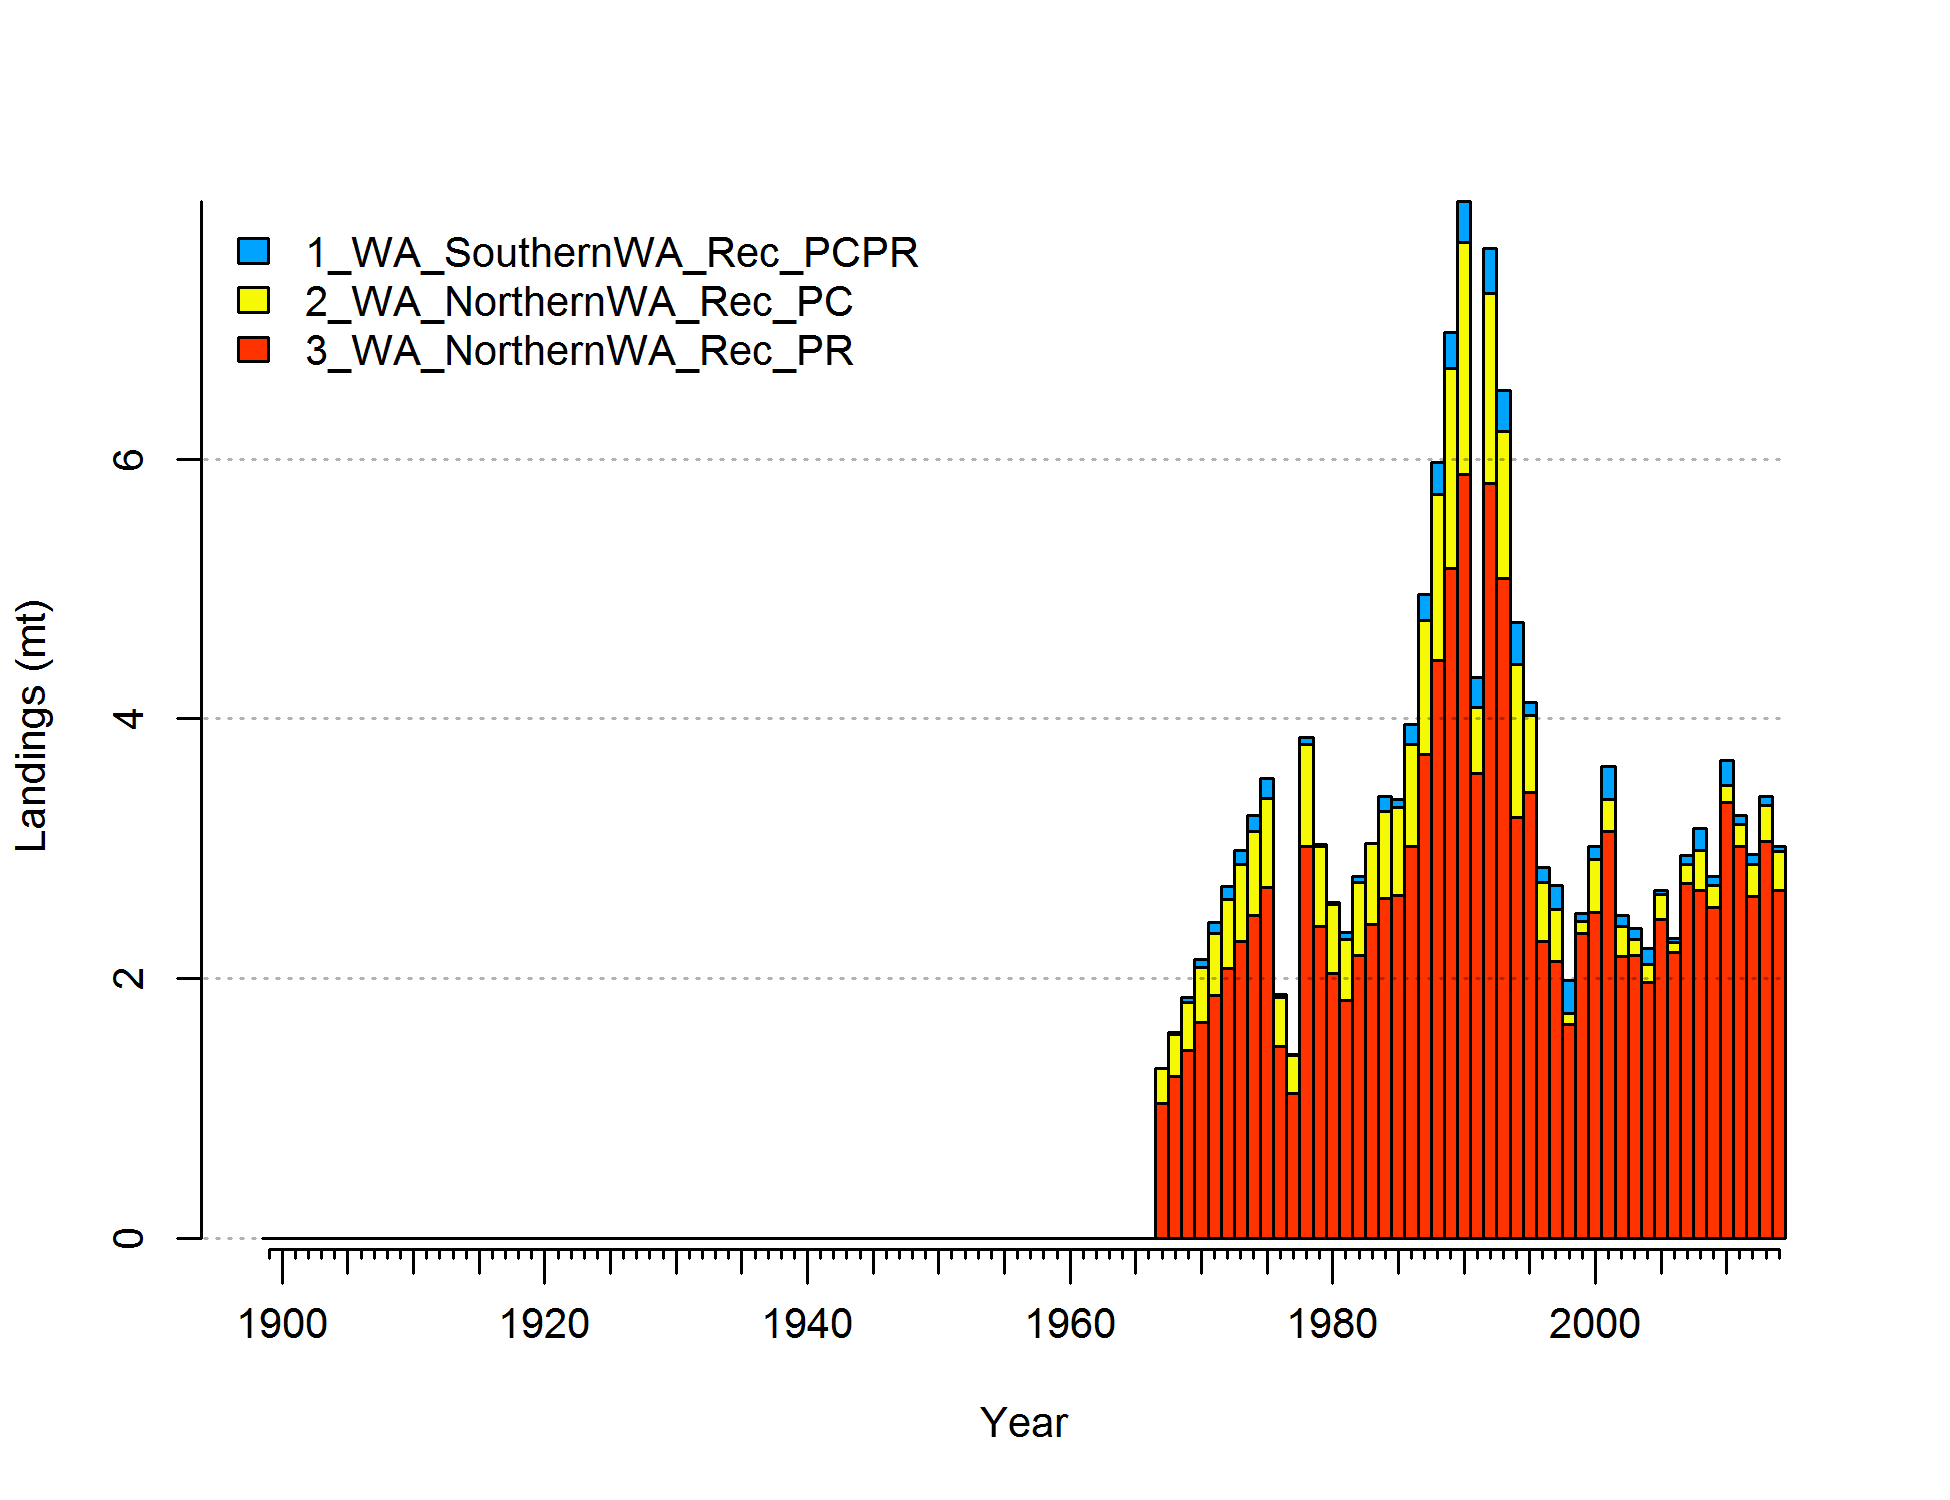
\includegraphics{r4ss/plots_mod1/catch2 landings stacked.png}
\caption{Total catches Pacific ocean perch through 2016.
\label{fig:Catch}}
\end{figure}

\FloatBarrier

\begin{figure}
\centering
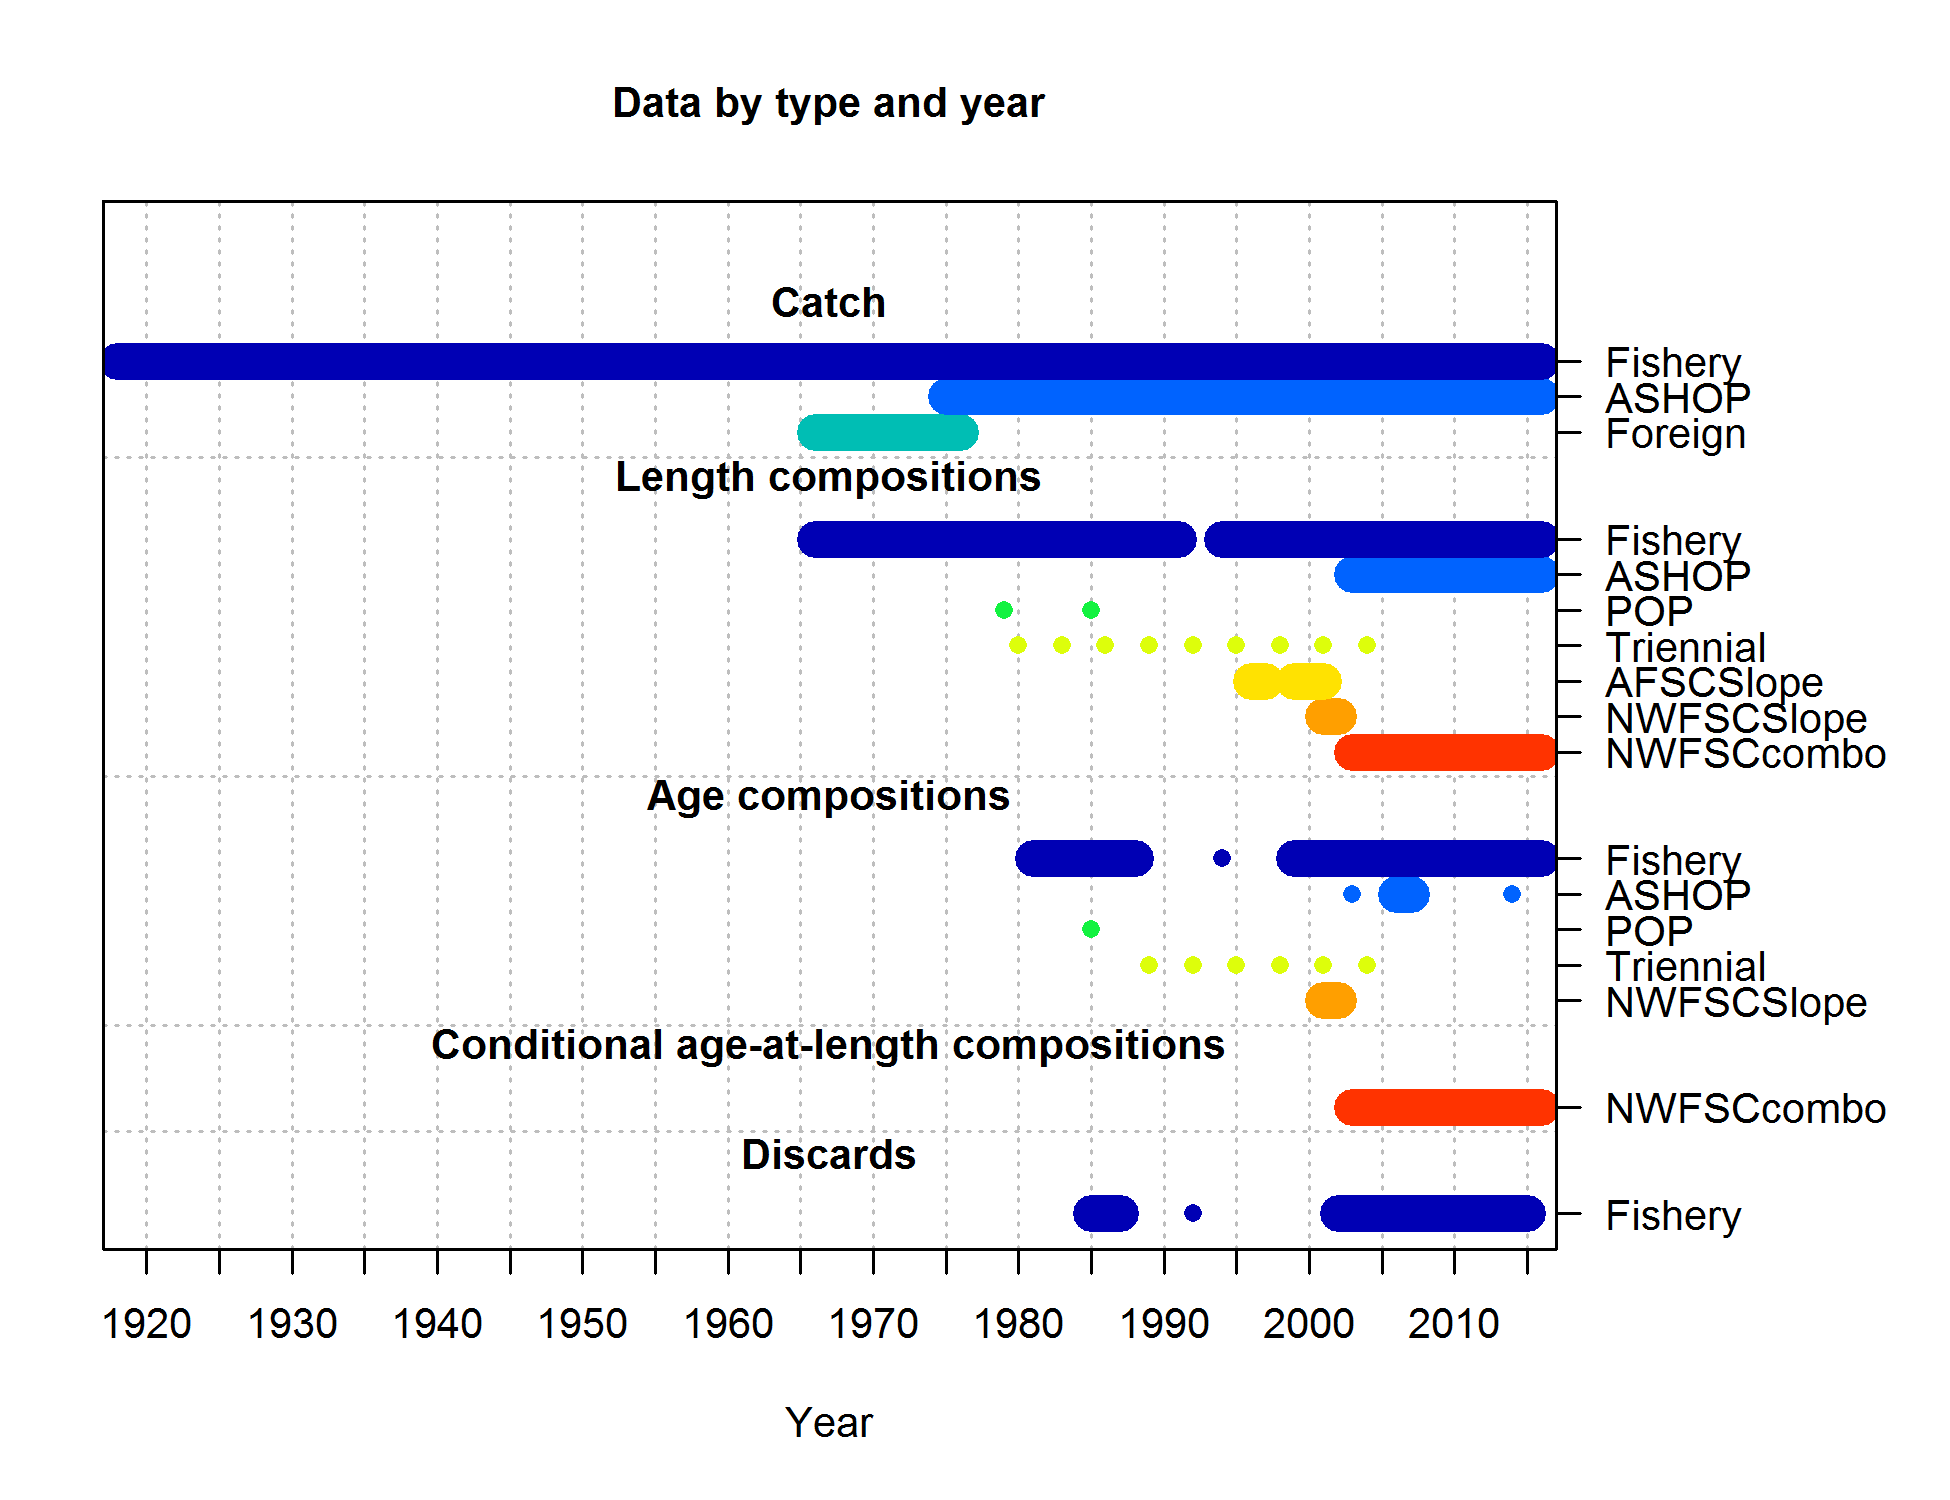
\includegraphics{r4ss/plots_mod1/data_plot.png}
\caption{Summary of data sources used in the base model.
\label{fig:data_plot}}
\end{figure}

\FloatBarrier

\begin{figure}
\centering
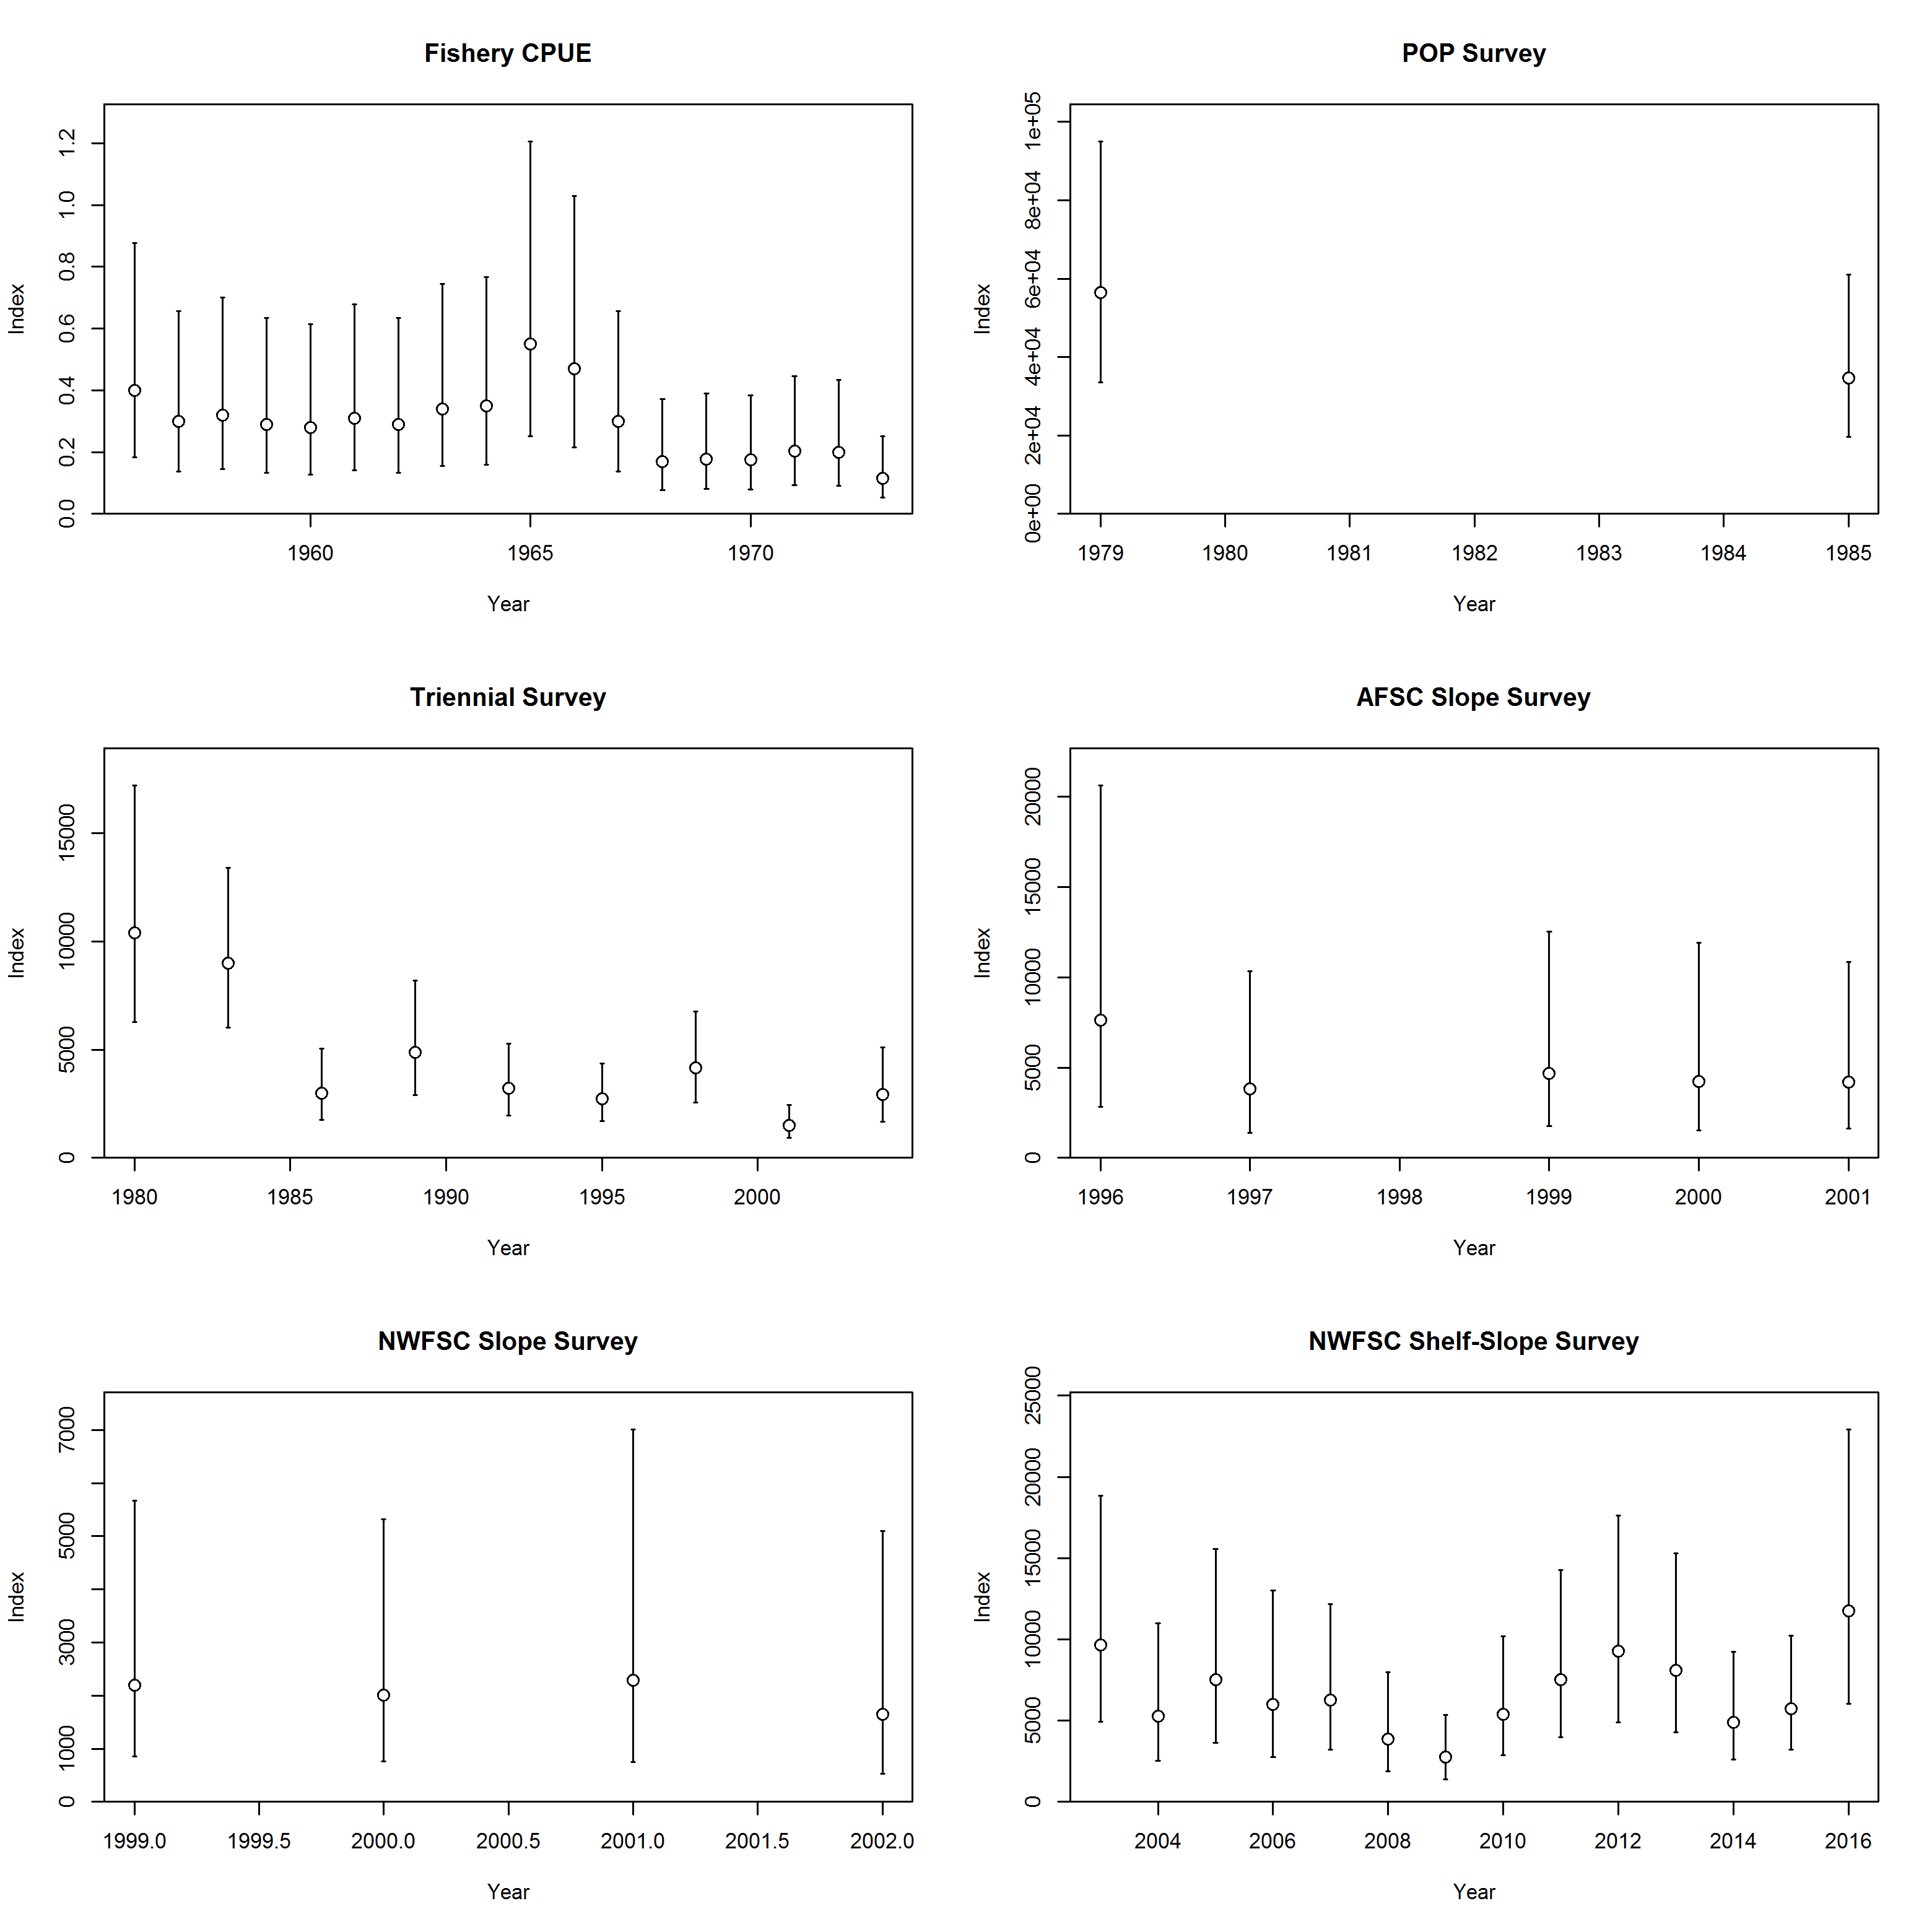
\includegraphics{Figures/Index_Data.png}
\caption{Fishery-dependent and fishery-independent indices for Pacific
ocean perch. \label{fig:indices}}
\end{figure}

\FloatBarrier

\begin{figure}
\centering
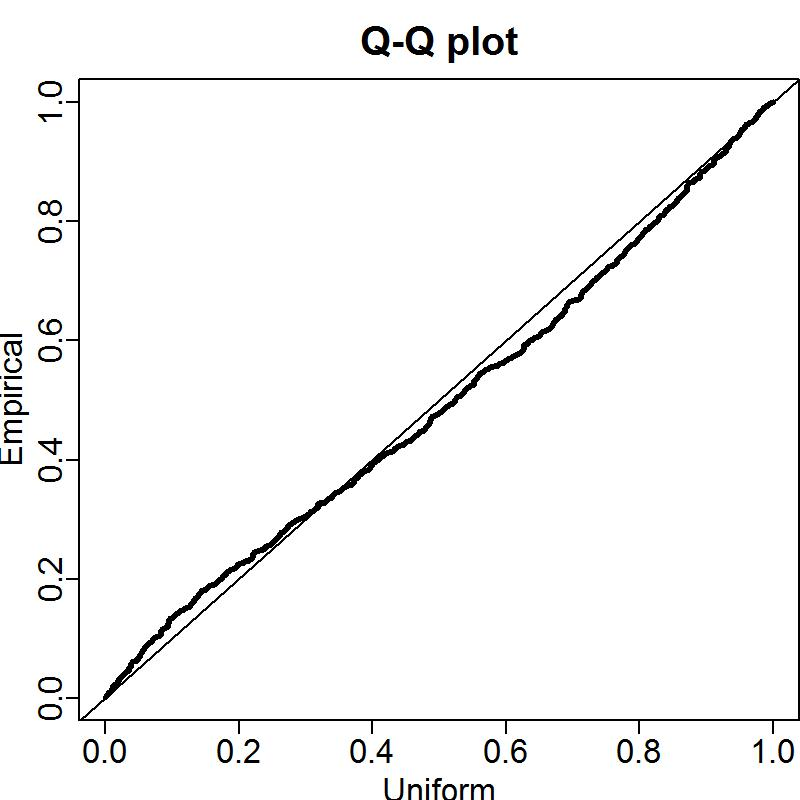
\includegraphics{Figures/Q-Q_plot_combo.jpg}
\caption{Q-Q plots for the VAST lognormal distribution for the NWFSC
shelf-slope survey. \label{fig:nw_qq}}
\end{figure}

\FloatBarrier

\begin{figure}
\centering
\includegraphics{r4ss/plots_mod1/comp_lendat_bubflt8mkt0.png}
\caption{NWFSC shelf-slope survey length frequency distributions for
Pacific ocean perch. \label{fig:nw_Length}}
\end{figure}

\FloatBarrier

\begin{figure}
\centering
\includegraphics{r4ss/plots_mod1/comp_gstagedat_bubflt8mkt0.png}
\caption{NWFSC shelf-slope survey age frequency distributions for
Pacific ocean perch. \label{fig:nw_Age}}
\end{figure}

\FloatBarrier

\begin{figure}
\centering
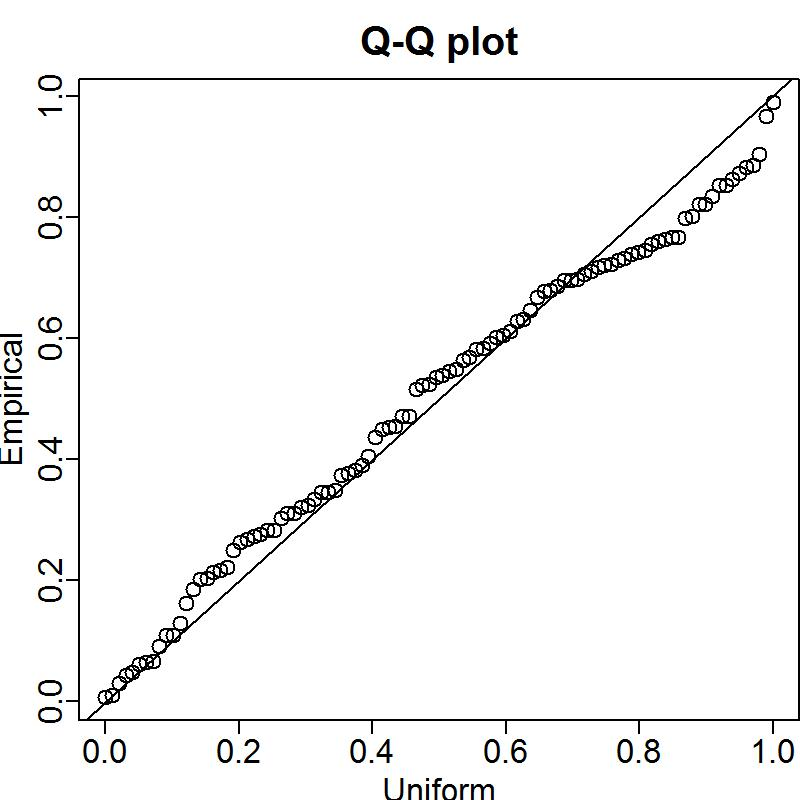
\includegraphics{Figures/Q-Q_plot_nw_slope_gammaECE.jpg}
\caption{Q-Q plots for the VAST lognormal distribution for the NWFSC
slope survey. \label{fig:nw_slope_qq}}
\end{figure}

\FloatBarrier

\begin{figure}
\centering
\includegraphics{r4ss/plots_mod1/comp_lendat_bubflt7mkt0.png}
\caption{NWFSC slope survey length frequency distributions for Pacific
ocean perch. \label{fig:nw_slope_Length}}
\end{figure}

\FloatBarrier

\begin{figure}
\centering
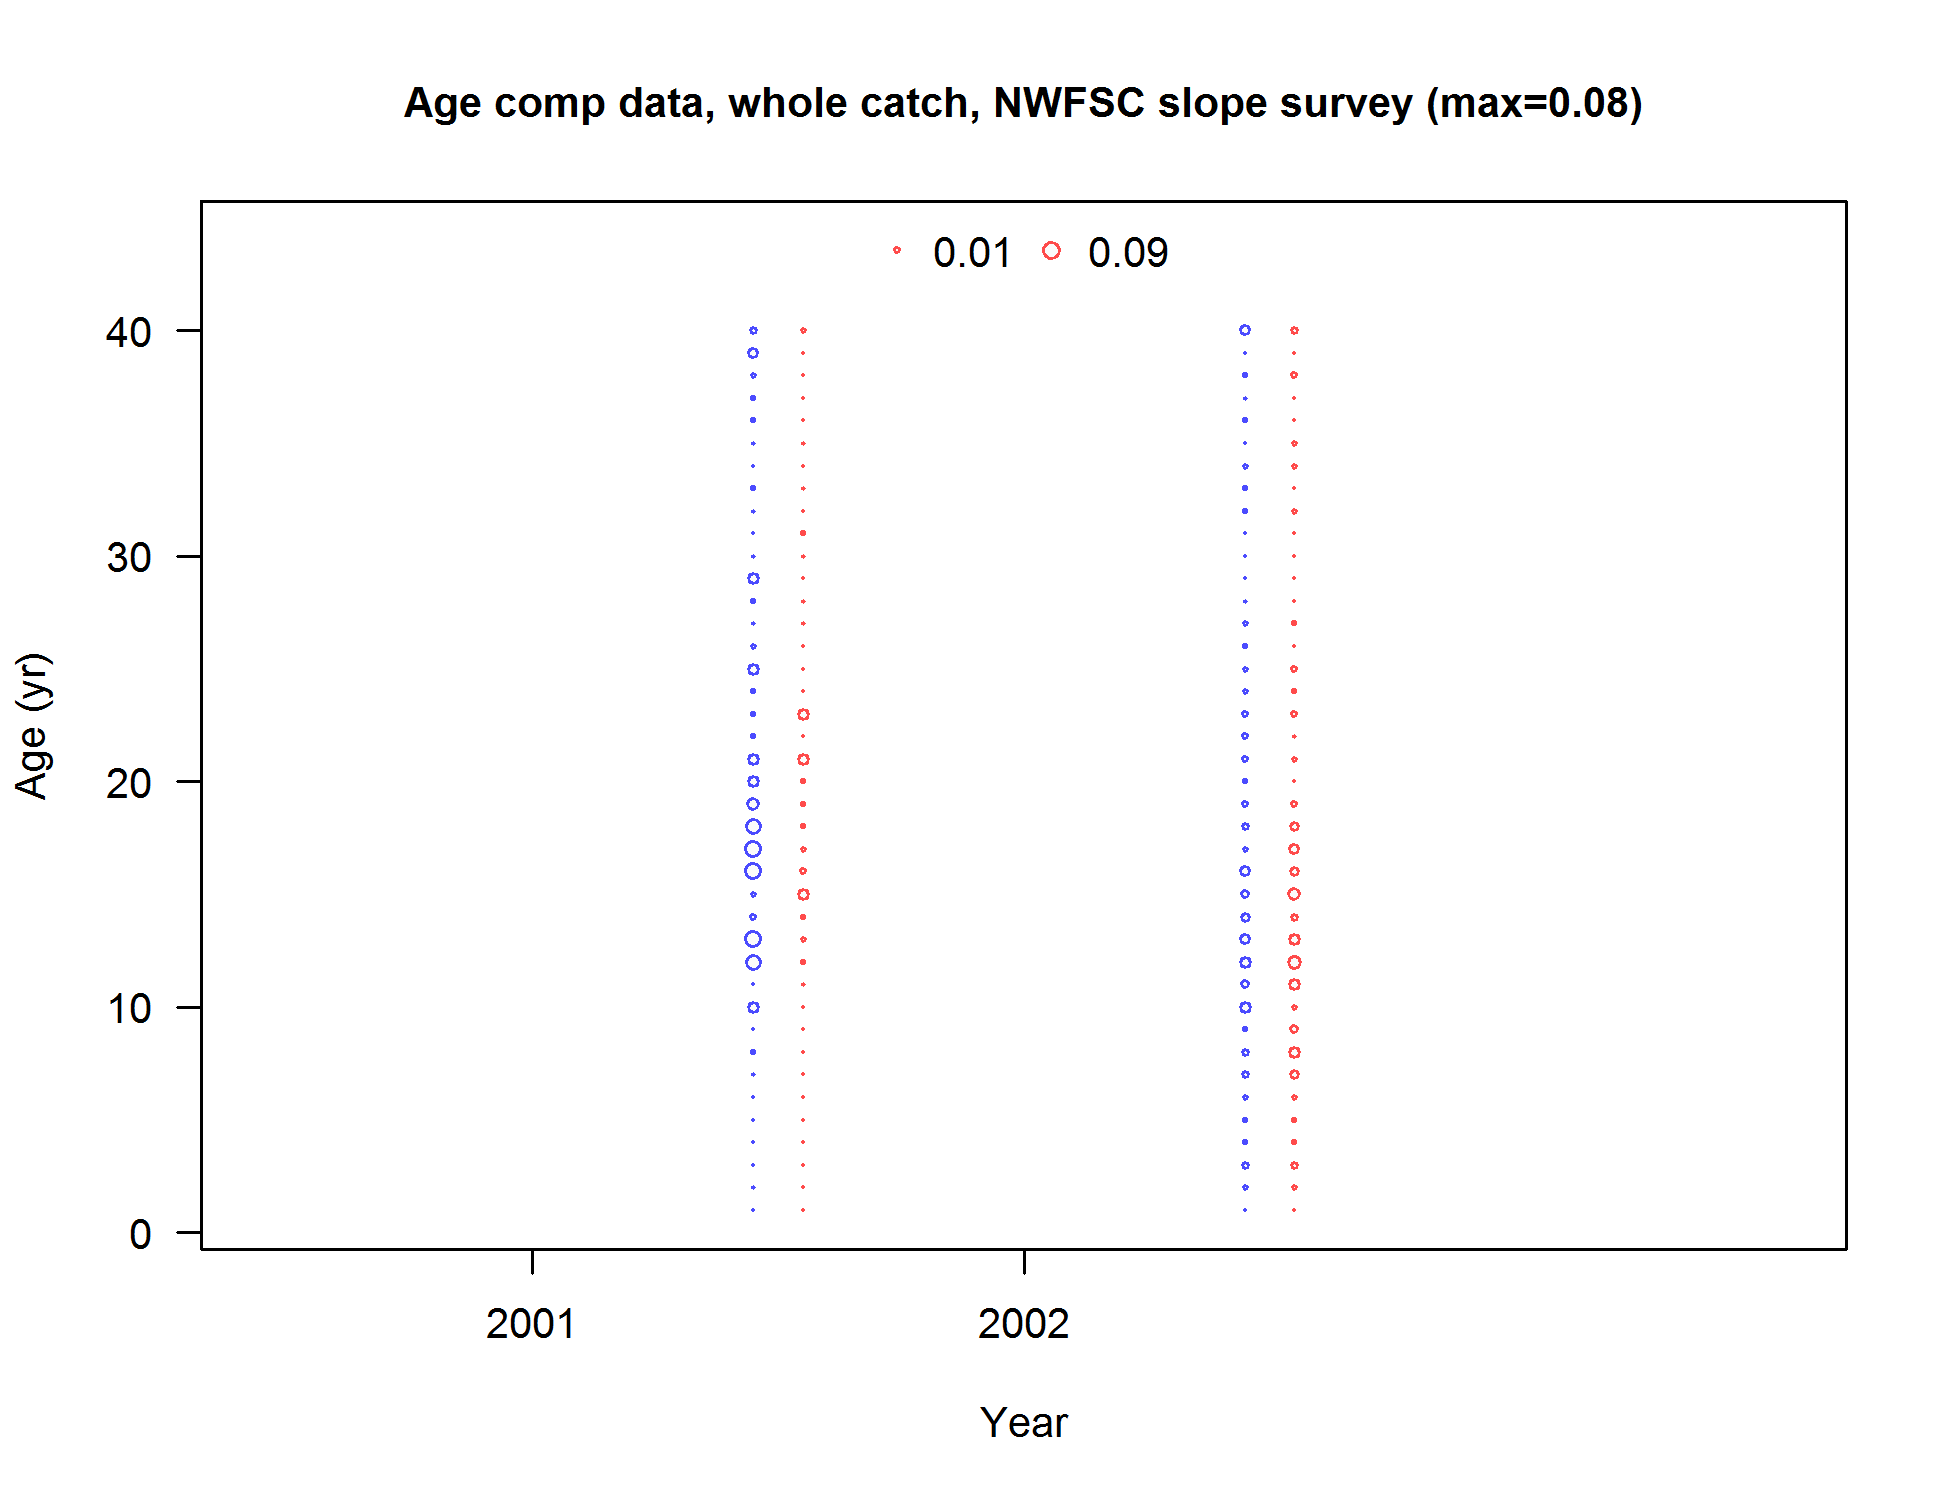
\includegraphics{r4ss/plots_mod1/comp_agedat_bubflt7mkt0.png}
\caption{NWFSC slope survey age frequency distributions for Pacific
ocean perch. \label{fig:nw_slope_Age}}
\end{figure}

\FloatBarrier

\begin{figure}
\centering
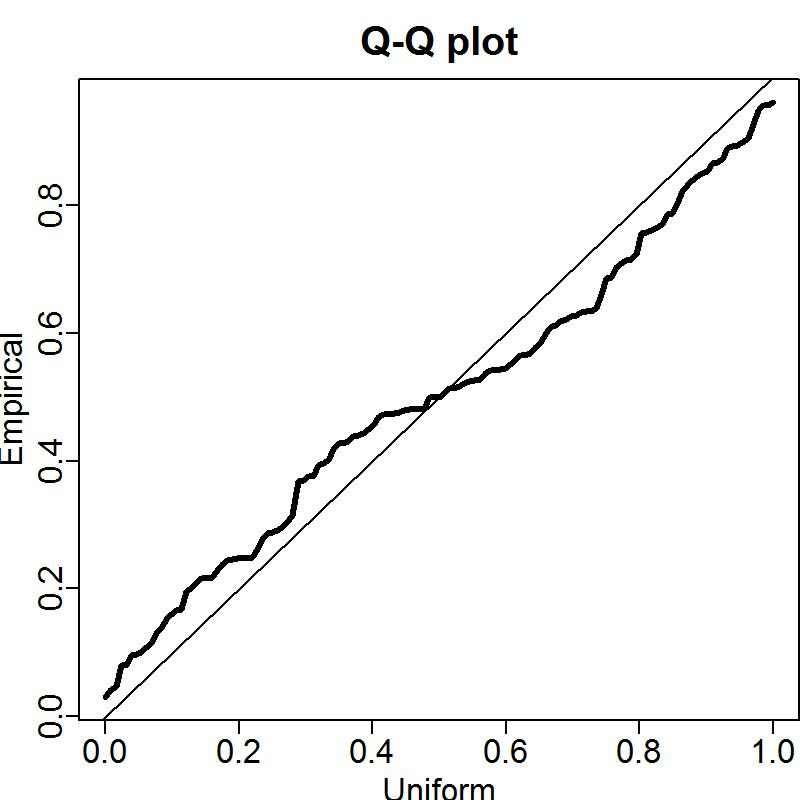
\includegraphics{Figures/Q-Q_plot_afsc.jpg}
\caption{Q-Q plots for the VAST lognormal distribution for the AFSC
slope survey. \label{fig:afsc_qq}}
\end{figure}

\FloatBarrier

\begin{figure}
\centering
\includegraphics{r4ss/plots_mod1/comp_lendat_bubflt6mkt0.png}
\caption{AFSC slope survey length frequency distributions for Pacific
ocean perch. \label{fig:afsc_Length}}
\end{figure}

\FloatBarrier

\begin{figure}
\centering
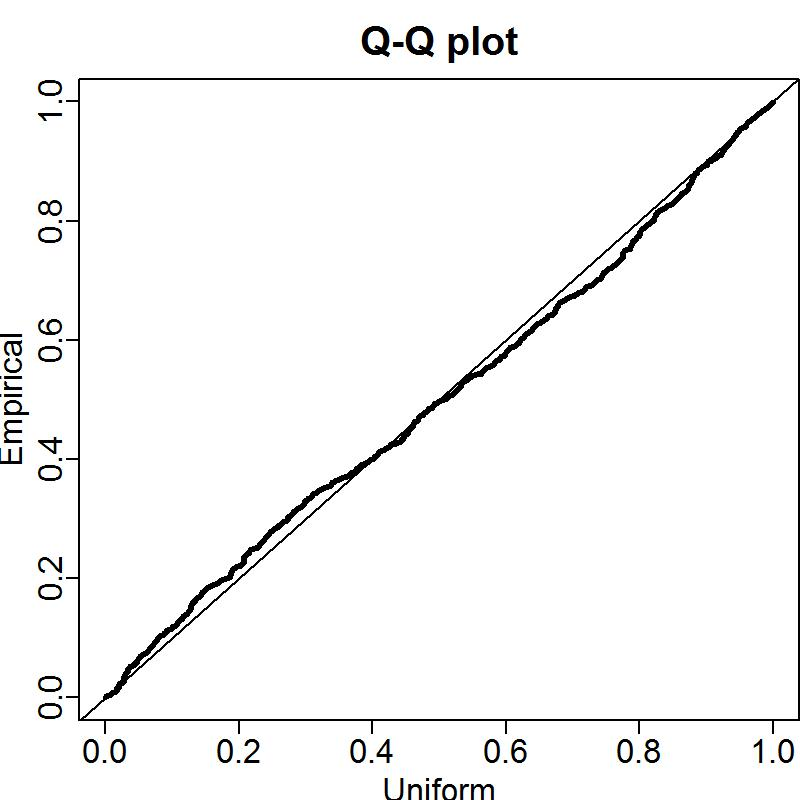
\includegraphics{Figures/Q-Q_plot_triennial.jpg}
\caption{Q-Q plots for the VAST lognormal distribution for the Triennial
survey. \label{fig:tri_qq}}
\end{figure}

\FloatBarrier

\begin{figure}
\centering
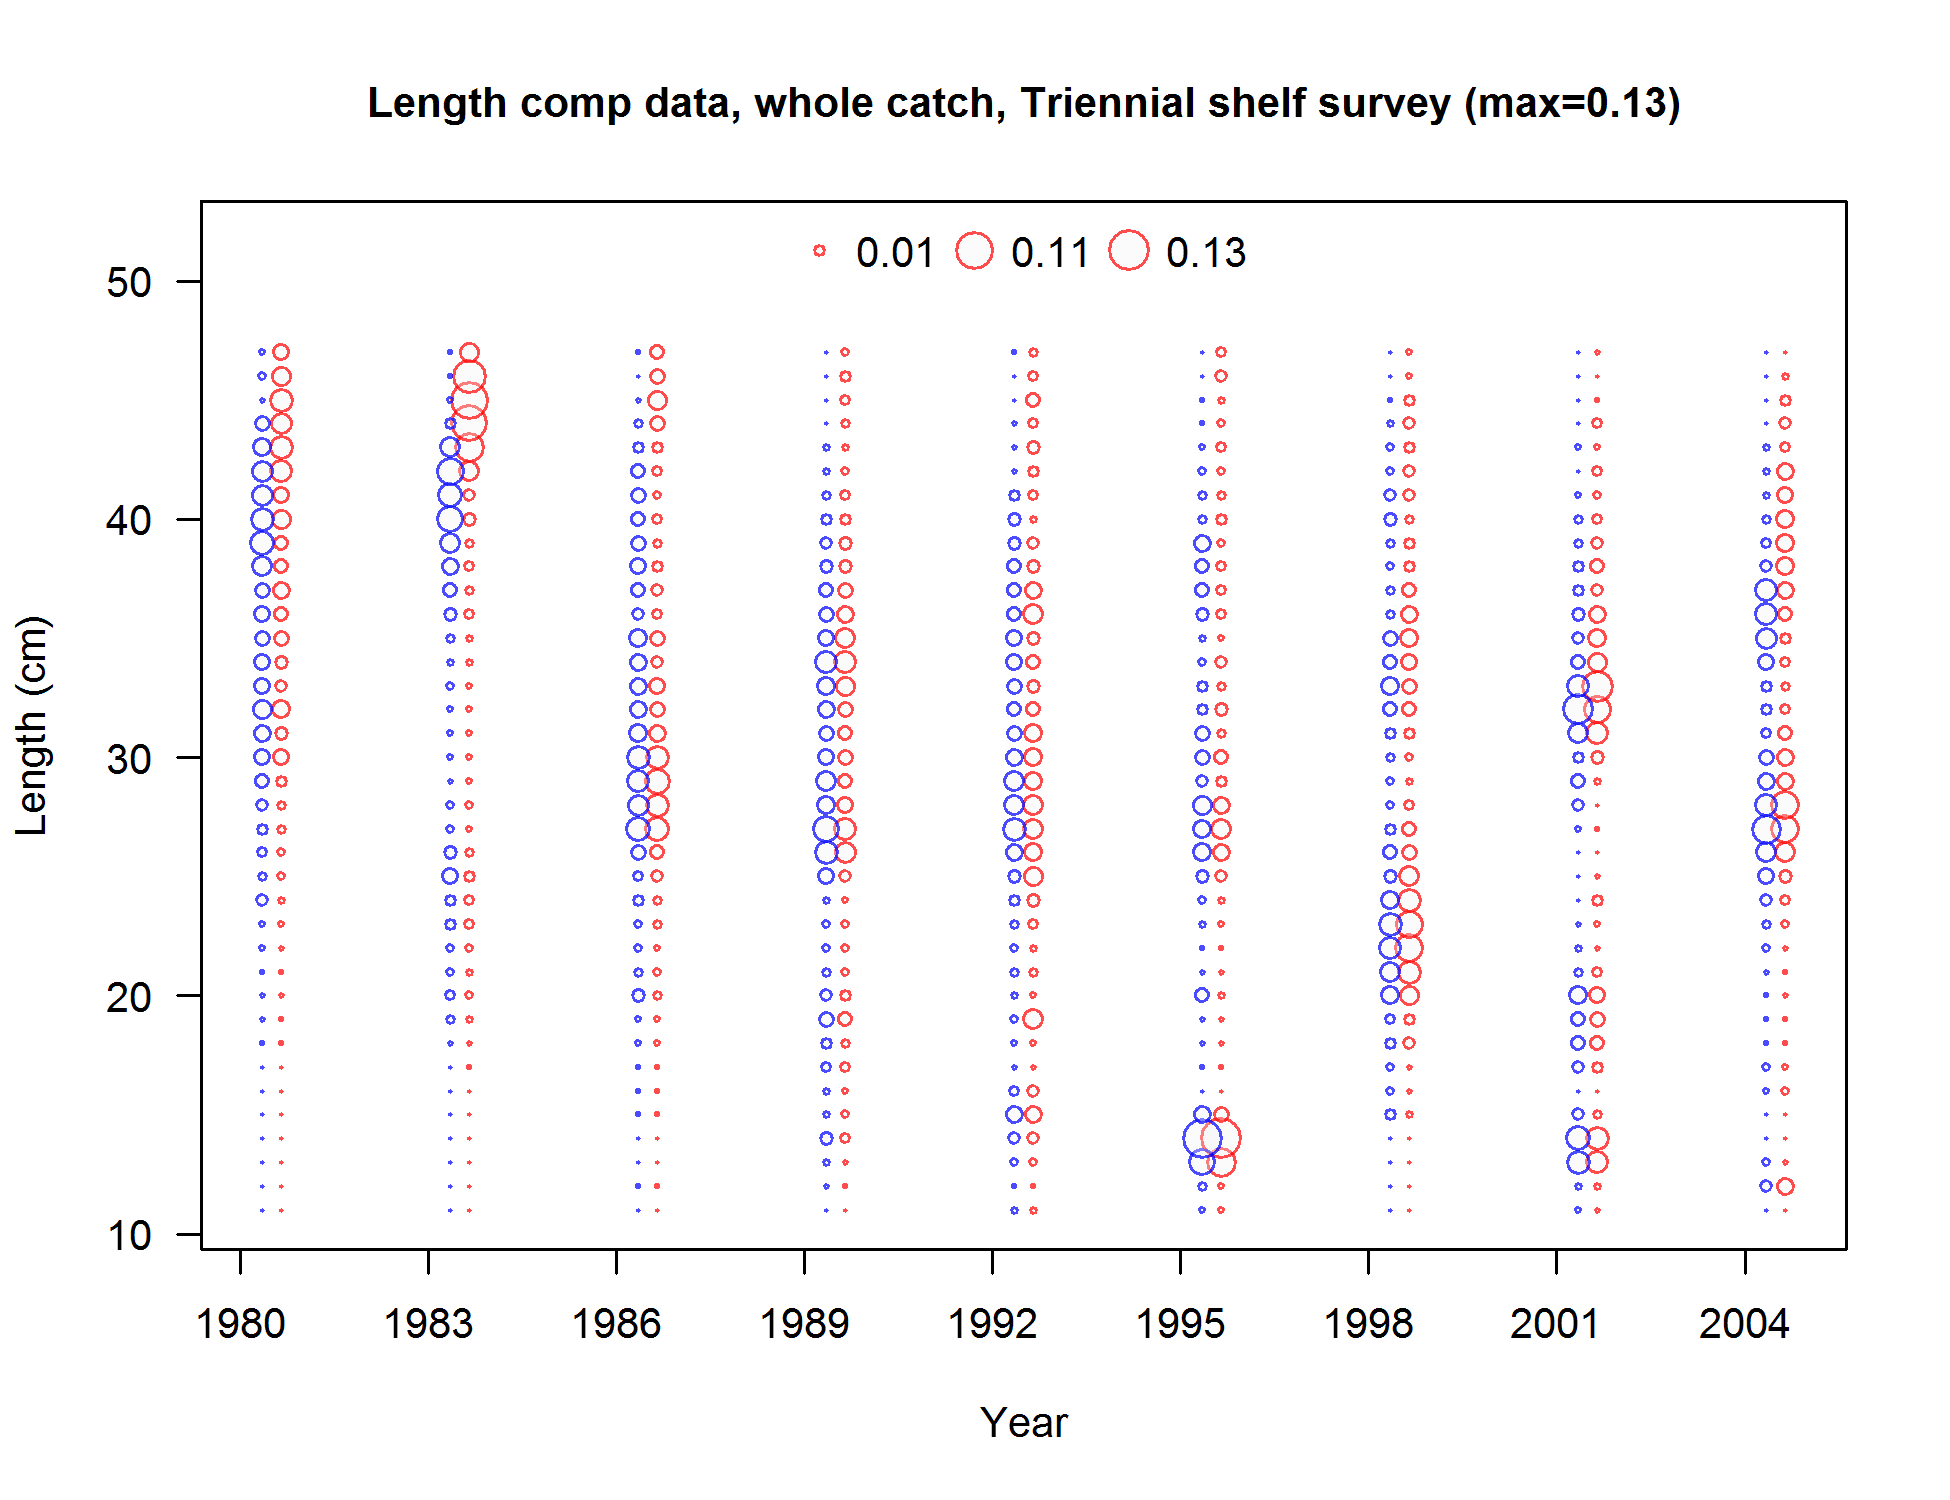
\includegraphics{r4ss/plots_mod1/comp_lendat_bubflt5mkt0.png}
\caption{Triennial survey length frequency distributions for Pacific
ocean perch. \label{fig:Tri_Length}}
\end{figure}

\FloatBarrier

\begin{figure}
\centering
\includegraphics{r4ss/plots_mod1/comp_agedat_bubflt5mkt0.png}
\caption{Triennial survey age frequency distributions for Pacific ocean
perch. \label{fig:Tri_Age}}
\end{figure}

\FloatBarrier

\begin{figure}
\centering
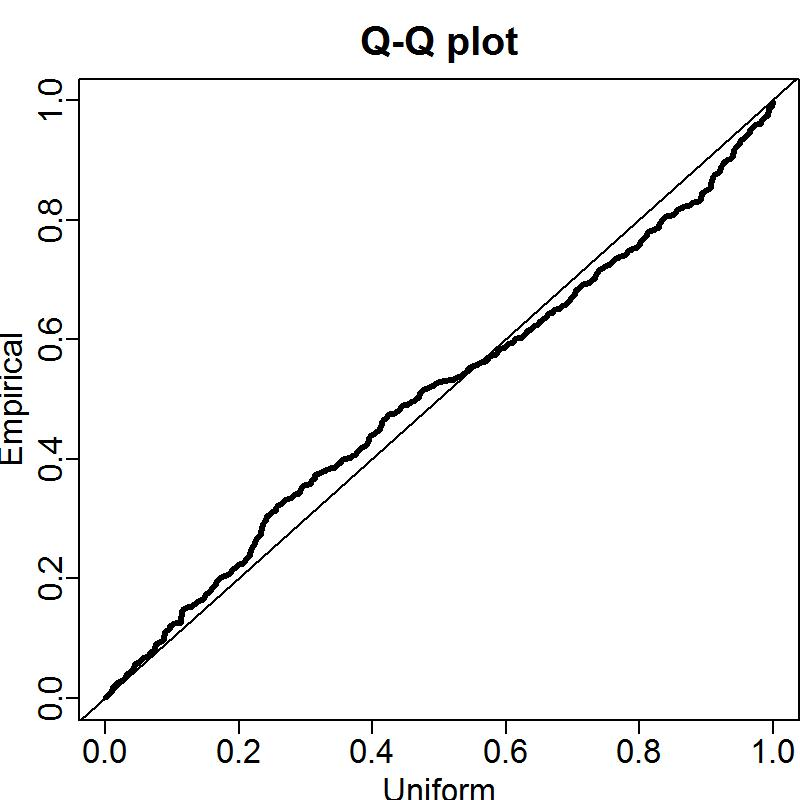
\includegraphics{Figures/Q-Q_plot_pop.jpg}
\caption{Q-Q plots for the VAST lognormal distribution for the Pacific
ocean perch survey. \label{fig:pop_qq}}
\end{figure}

\FloatBarrier

\begin{figure}
\centering
\includegraphics{r4ss/plots_mod1/comp_lendat_bubflt4mkt0.png}
\caption{Pacific ocean perch survey length frequency distributions for
Pacific ocean perch. \label{fig:POP_Length}}
\end{figure}

\FloatBarrier

\begin{figure}
\centering
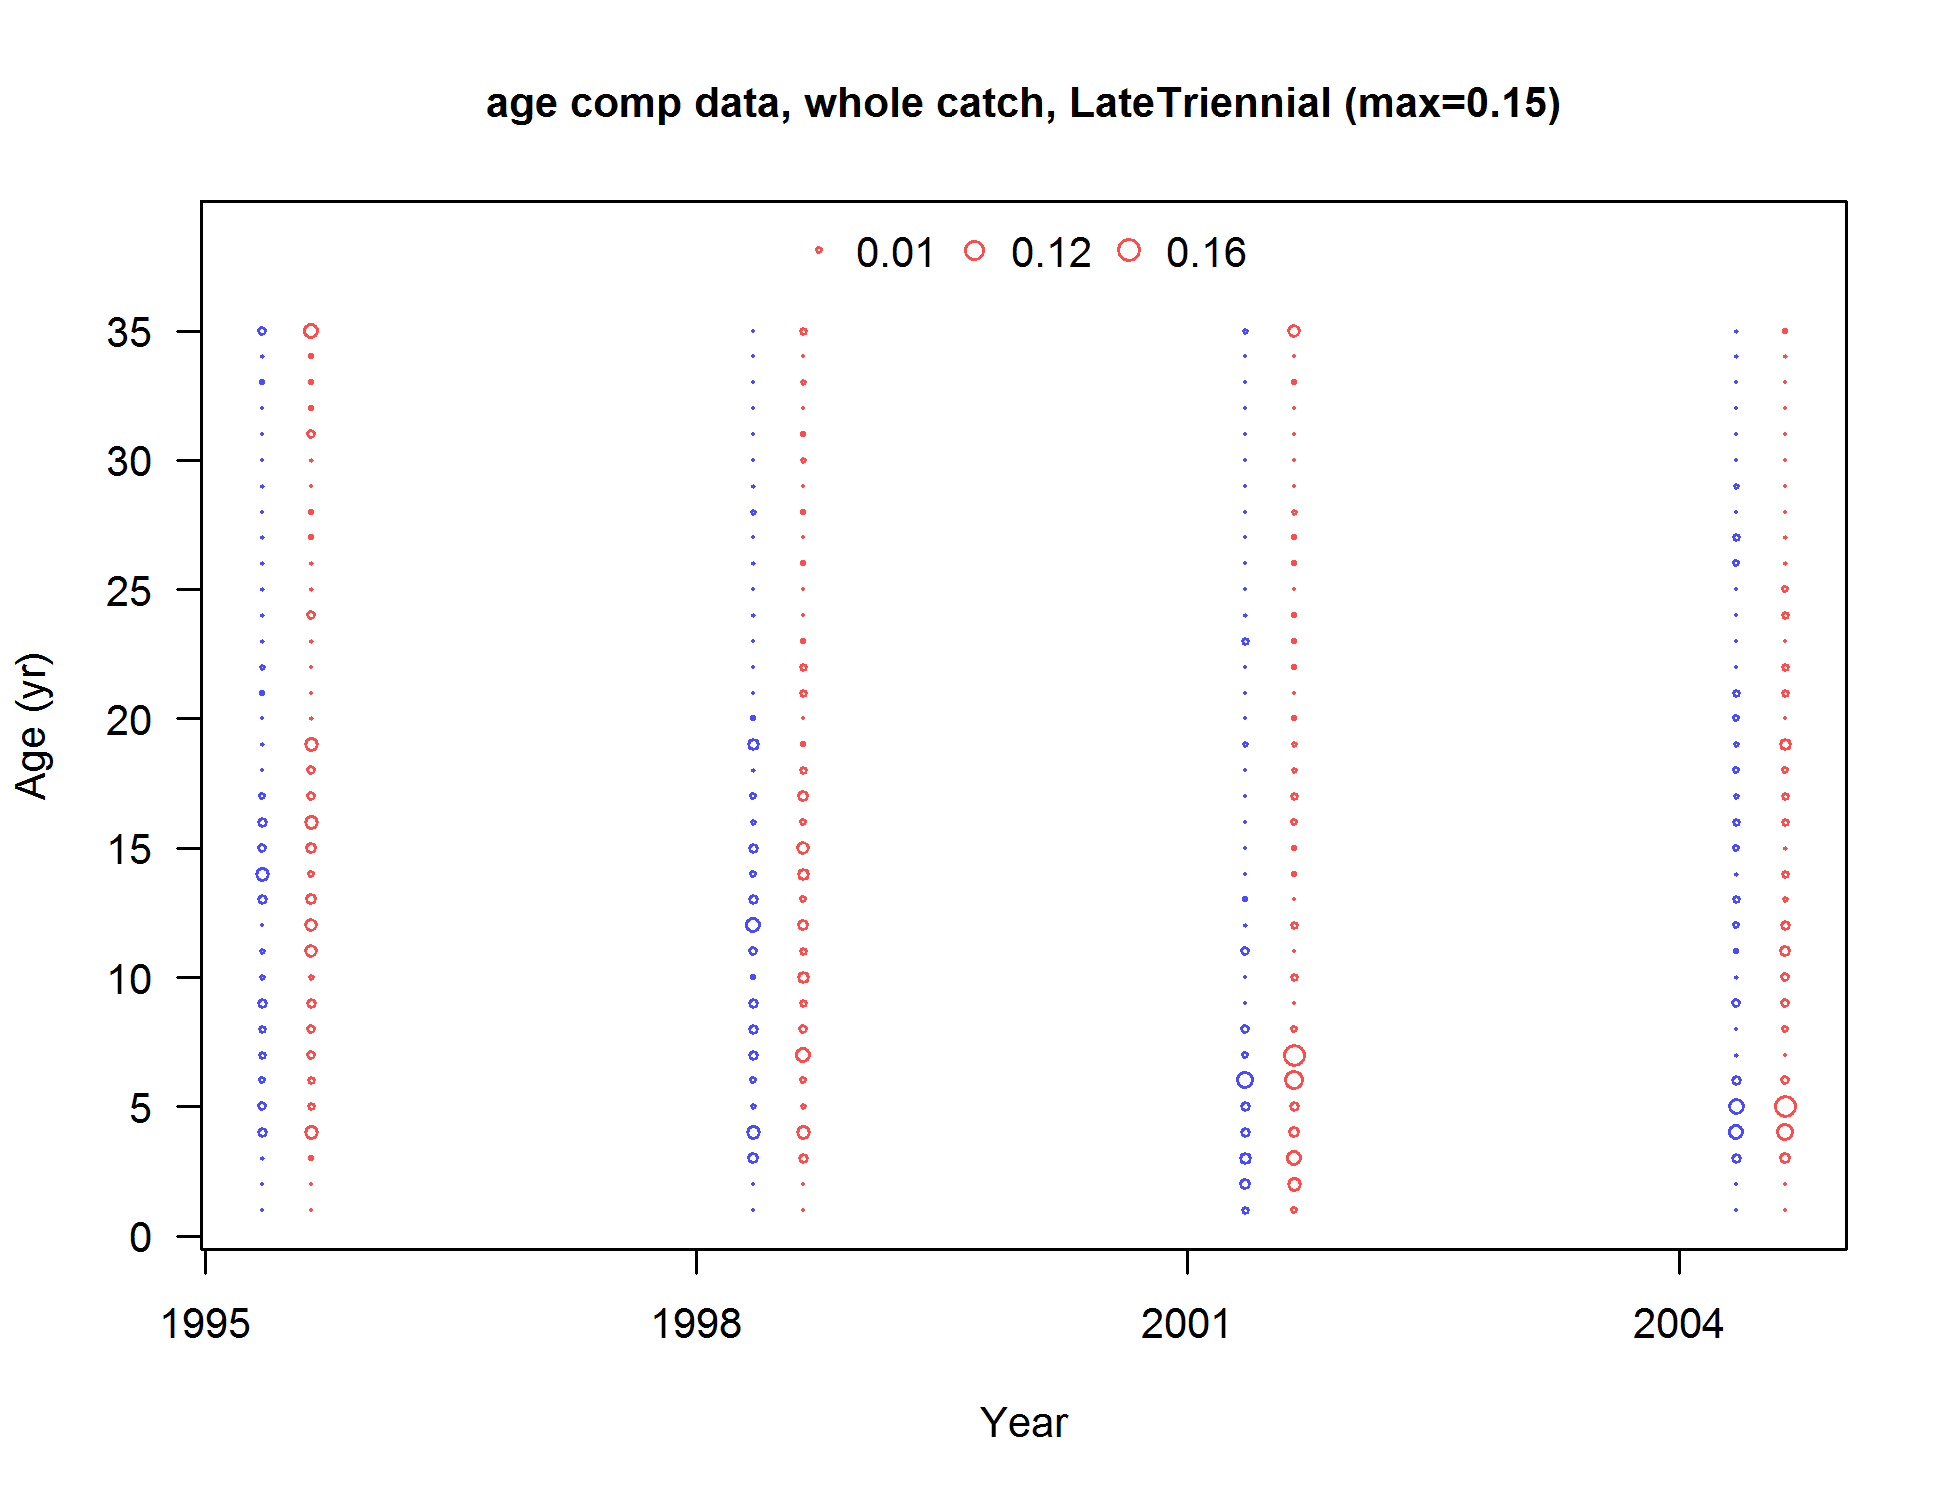
\includegraphics{r4ss/plots_mod1/comp_agedat_bubflt4mkt0.png}
\caption{Pacific ocean perch survey age frequency distributions for
Pacific ocean perch. \label{fig:POP_Age}}
\end{figure}

\FloatBarrier

\begin{figure}
\centering
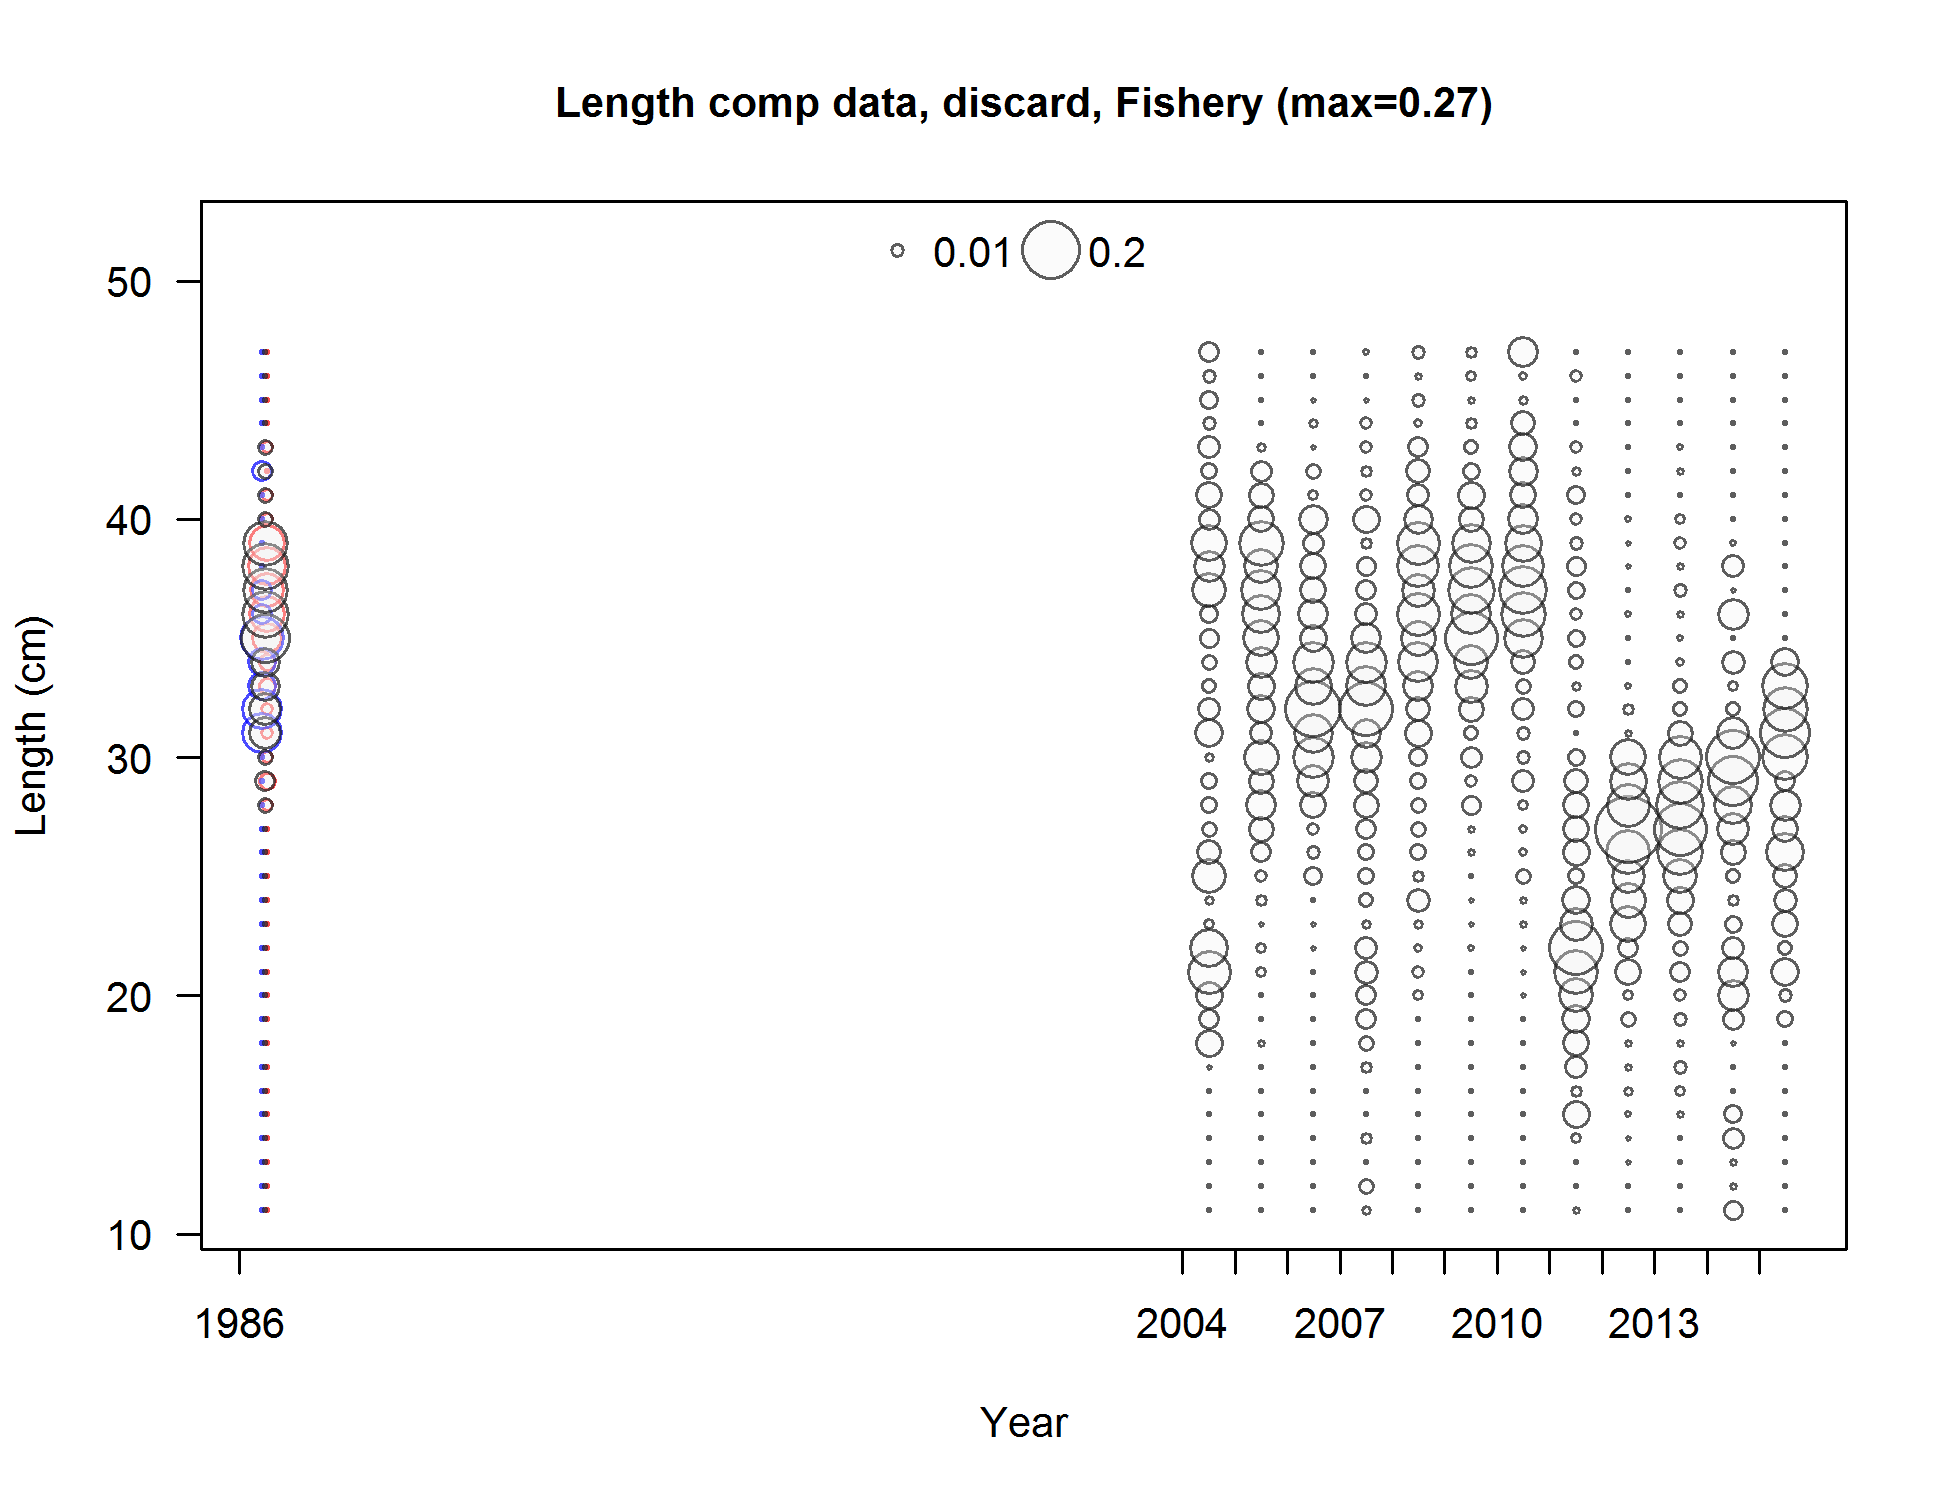
\includegraphics{r4ss/plots_mod1/comp_lendat_bubflt1mkt1.png}
\caption{Discard length frequency distributions from WCGOP for Pacific
ocean perch. \label{fig:WCGOP_discard}}
\end{figure}

\FloatBarrier

\begin{figure}
\centering
\includegraphics{r4ss/plots_mod1/comp_lendat_bubflt1mkt2_page4.png}
\caption{Commercial fishery length frequency distributions for Pacific
ocean perch. \label{fig:Comm_Length}}
\end{figure}

\FloatBarrier

\begin{figure}
\centering
\includegraphics{r4ss/plots_mod1/comp_agedat_bubflt1mkt2_page2.png}
\caption{Commercial fishery age frequency distributions for Pacific
ocean perch. \label{fig:Comm_Age}}
\end{figure}

\FloatBarrier

\begin{figure}
\centering
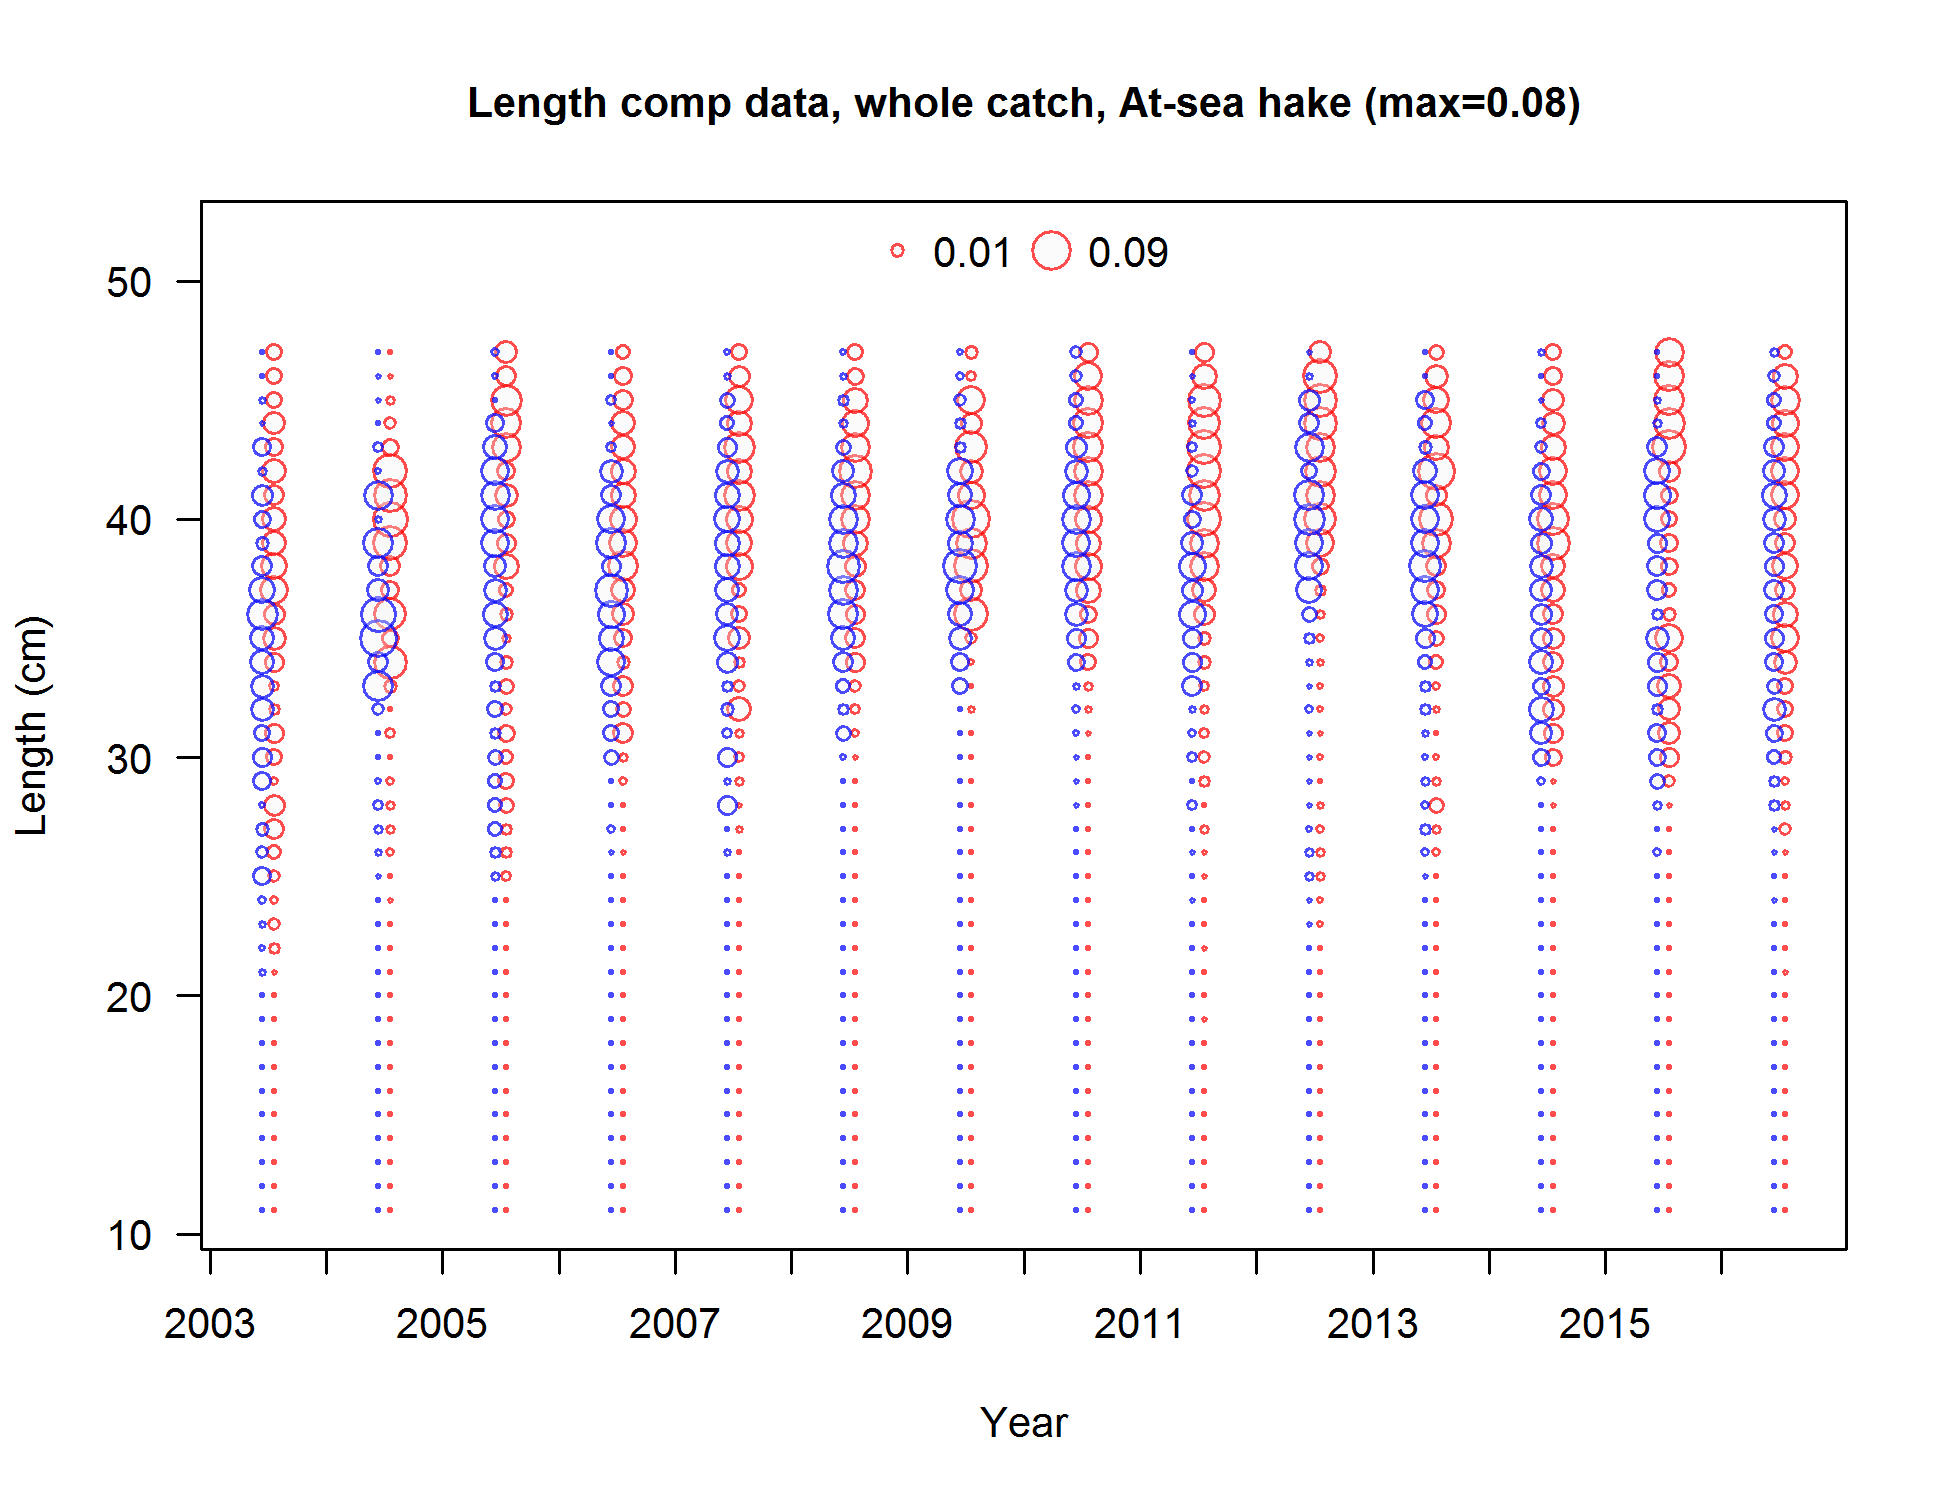
\includegraphics{r4ss/plots_mod1/comp_lendat_bubflt2mkt0.png}
\caption{At-Sea hake fishery length frequency distributions for Pacific
ocean perch. \label{fig:ASHOP_Length}}
\end{figure}

\FloatBarrier

\begin{figure}
\centering
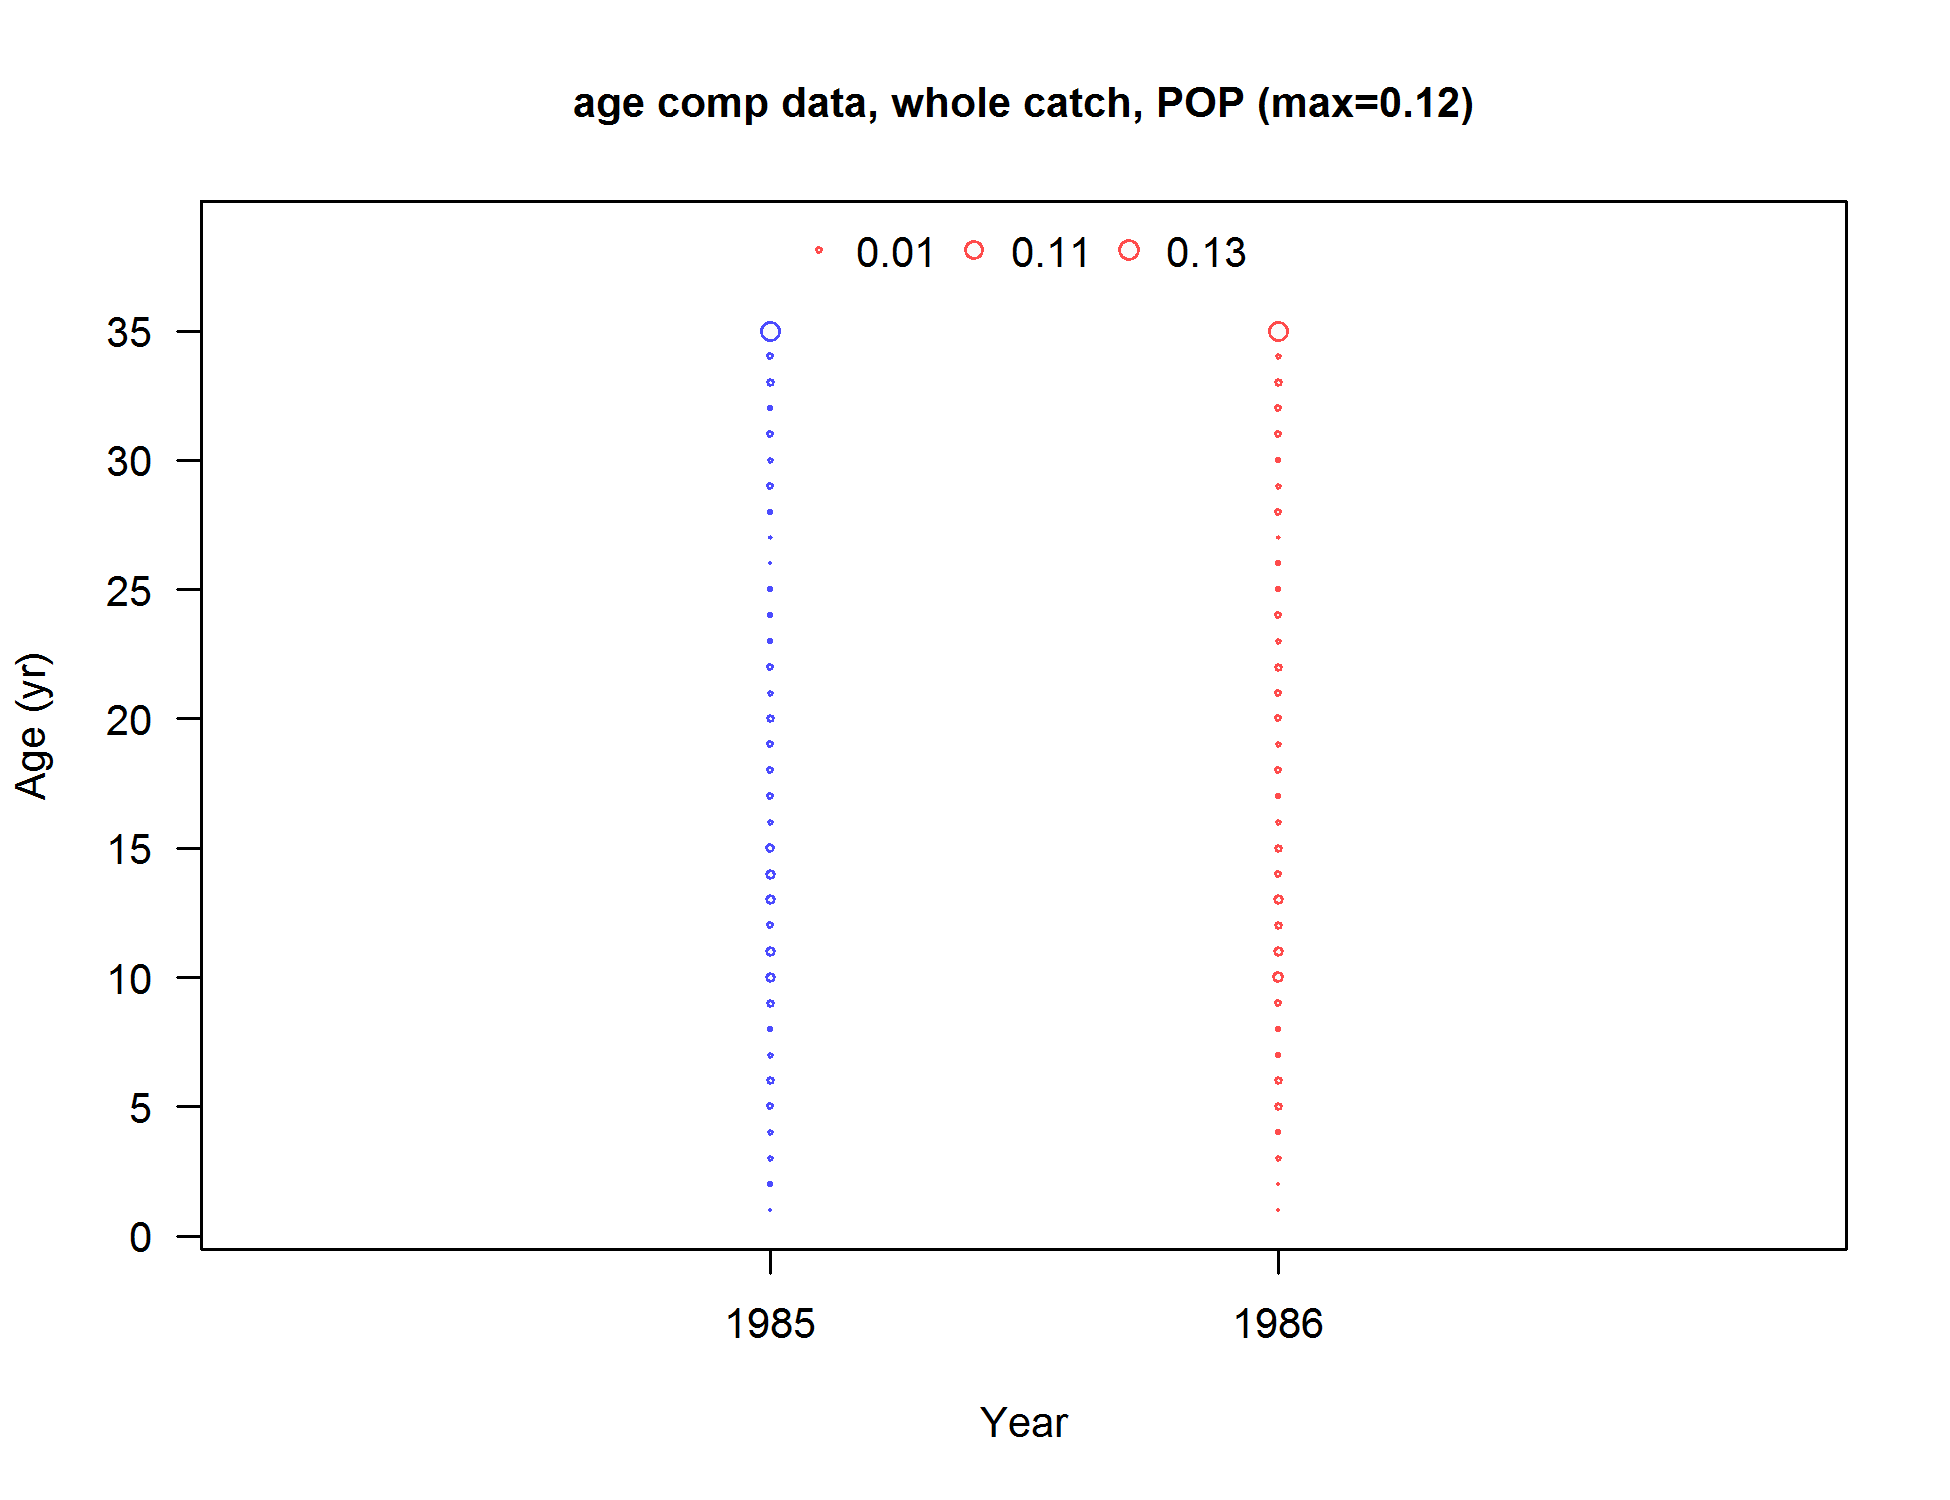
\includegraphics{r4ss/plots_mod1/comp_agedat_bubflt2mkt0.png}
\caption{At-Sea hake fishery age frequency distributions for Pacific
ocean perch. \label{fig:ASHOP_Age}}
\end{figure}

\FloatBarrier

\begin{figure}
\centering
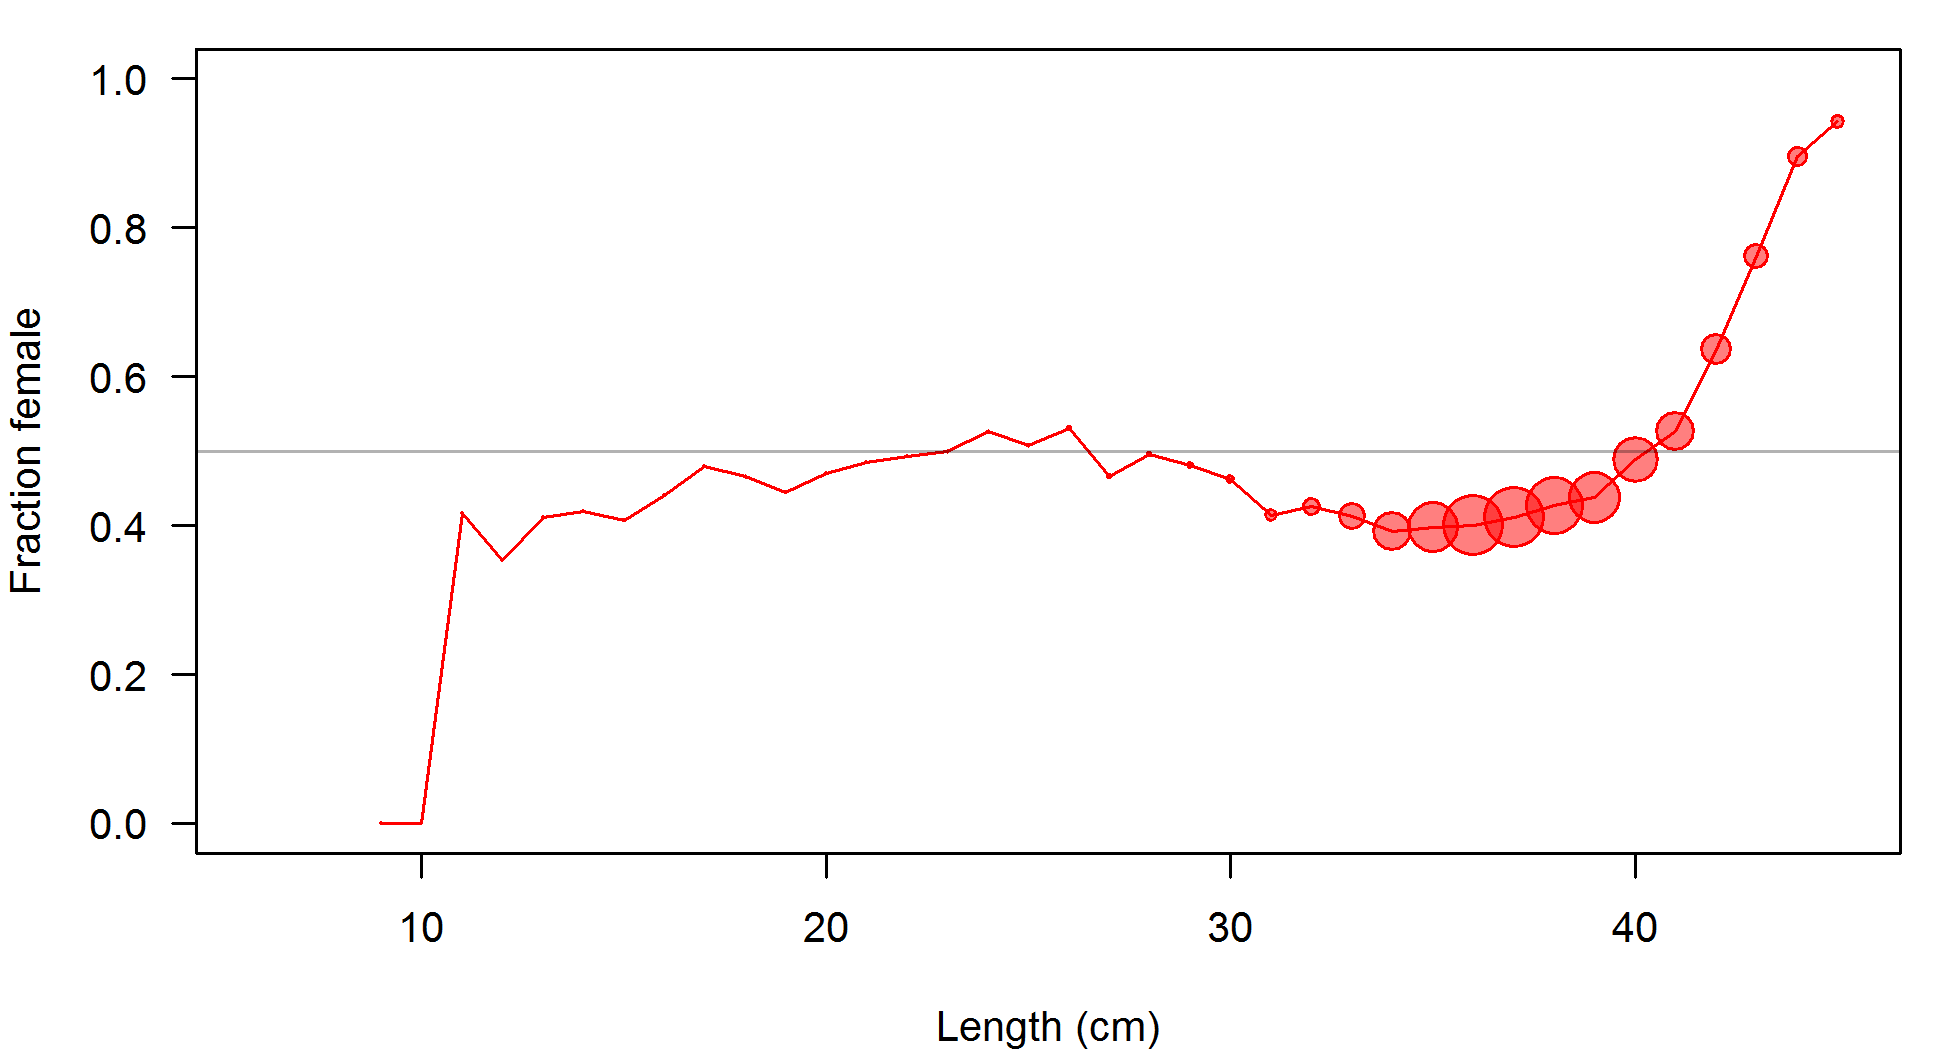
\includegraphics{Figures/allSexRatios.png}
\caption{The estimated sex ratio of Pacific ocean perch at length from
all biological data sources. \label{fig:sexratio}}
\end{figure}

\begin{figure}
\centering
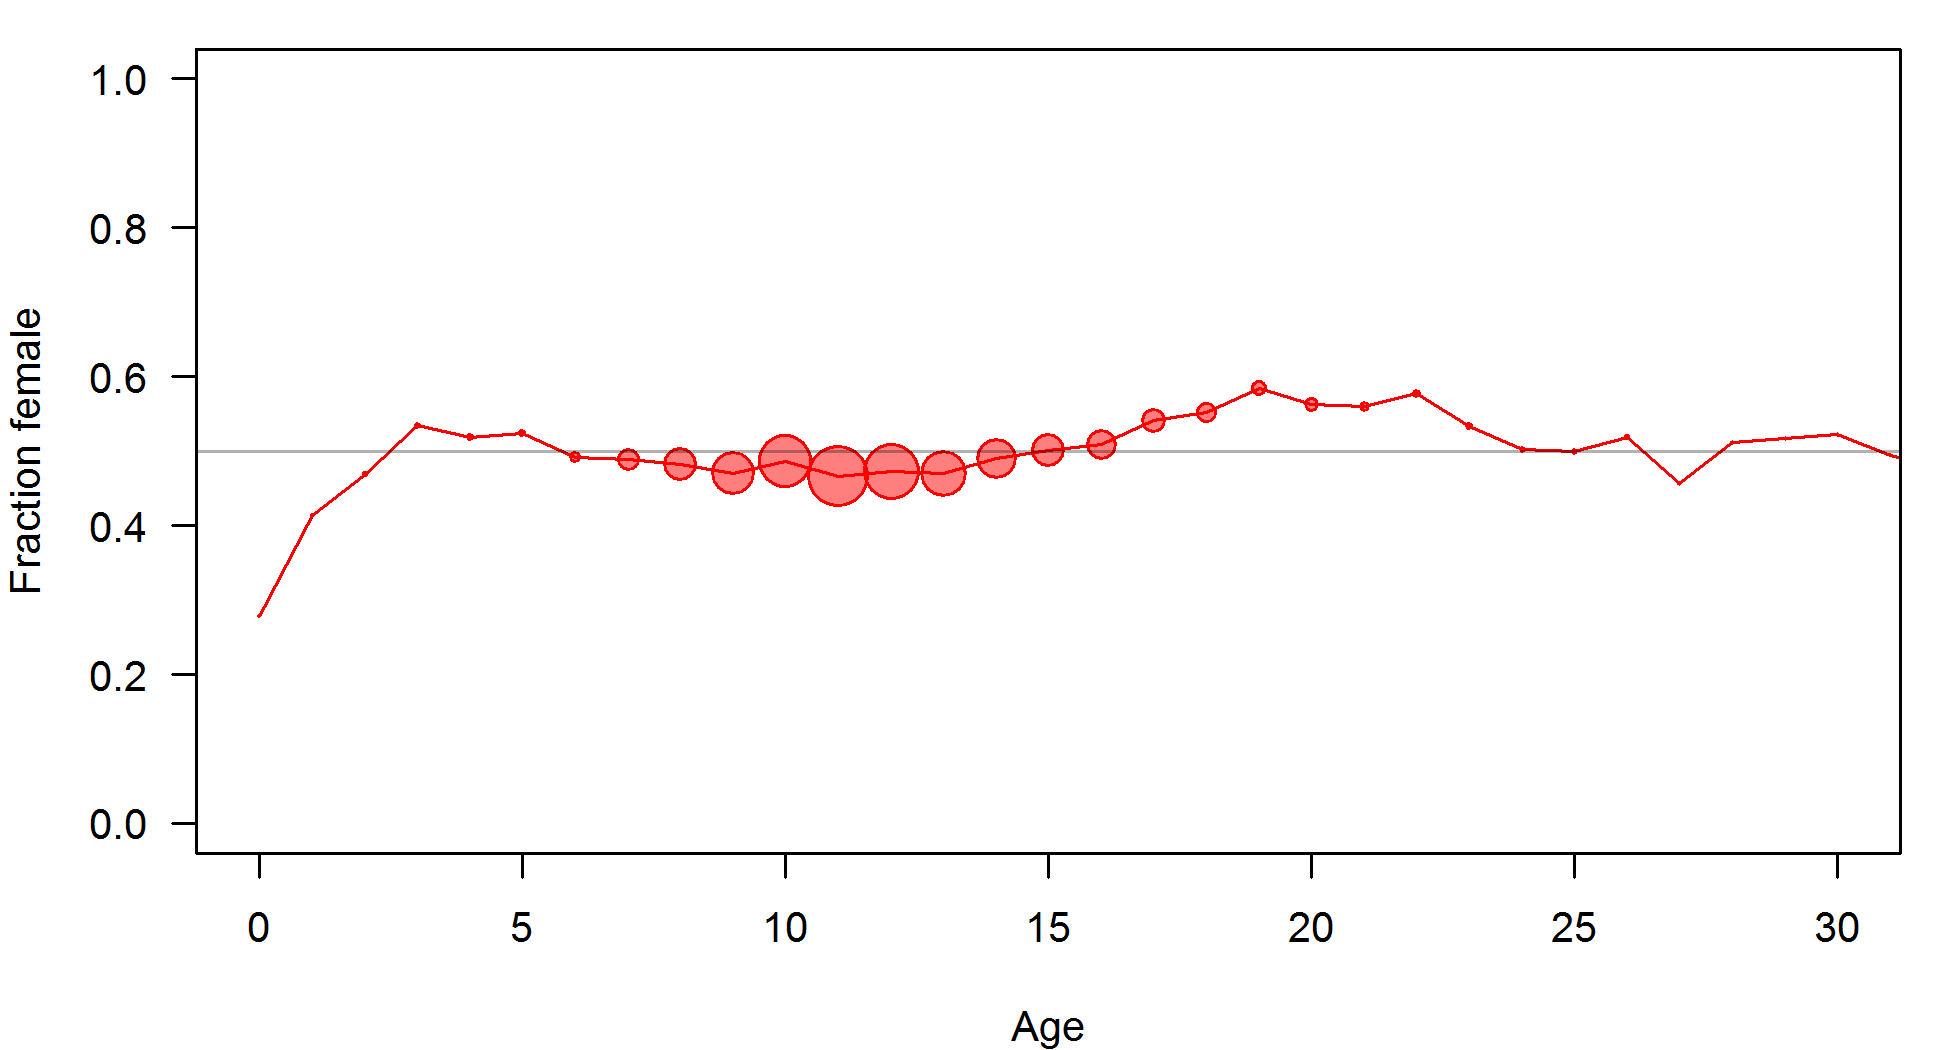
\includegraphics{Figures/allSexRatiosAge.png}
\caption{The estimated sex ratio of Pacific ocean perch at age from all
biological data sources. \label{fig:sexratio_Age}}
\end{figure}

\begin{figure}
\centering
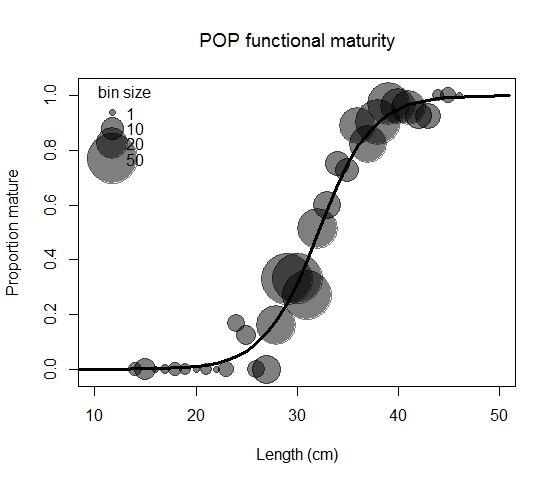
\includegraphics{Figures/Functional_Maturity.png}
\caption{The estimated functional maturity of Pacific ocean perch at
length. \label{fig:mat}}
\end{figure}

\begin{figure}
\centering
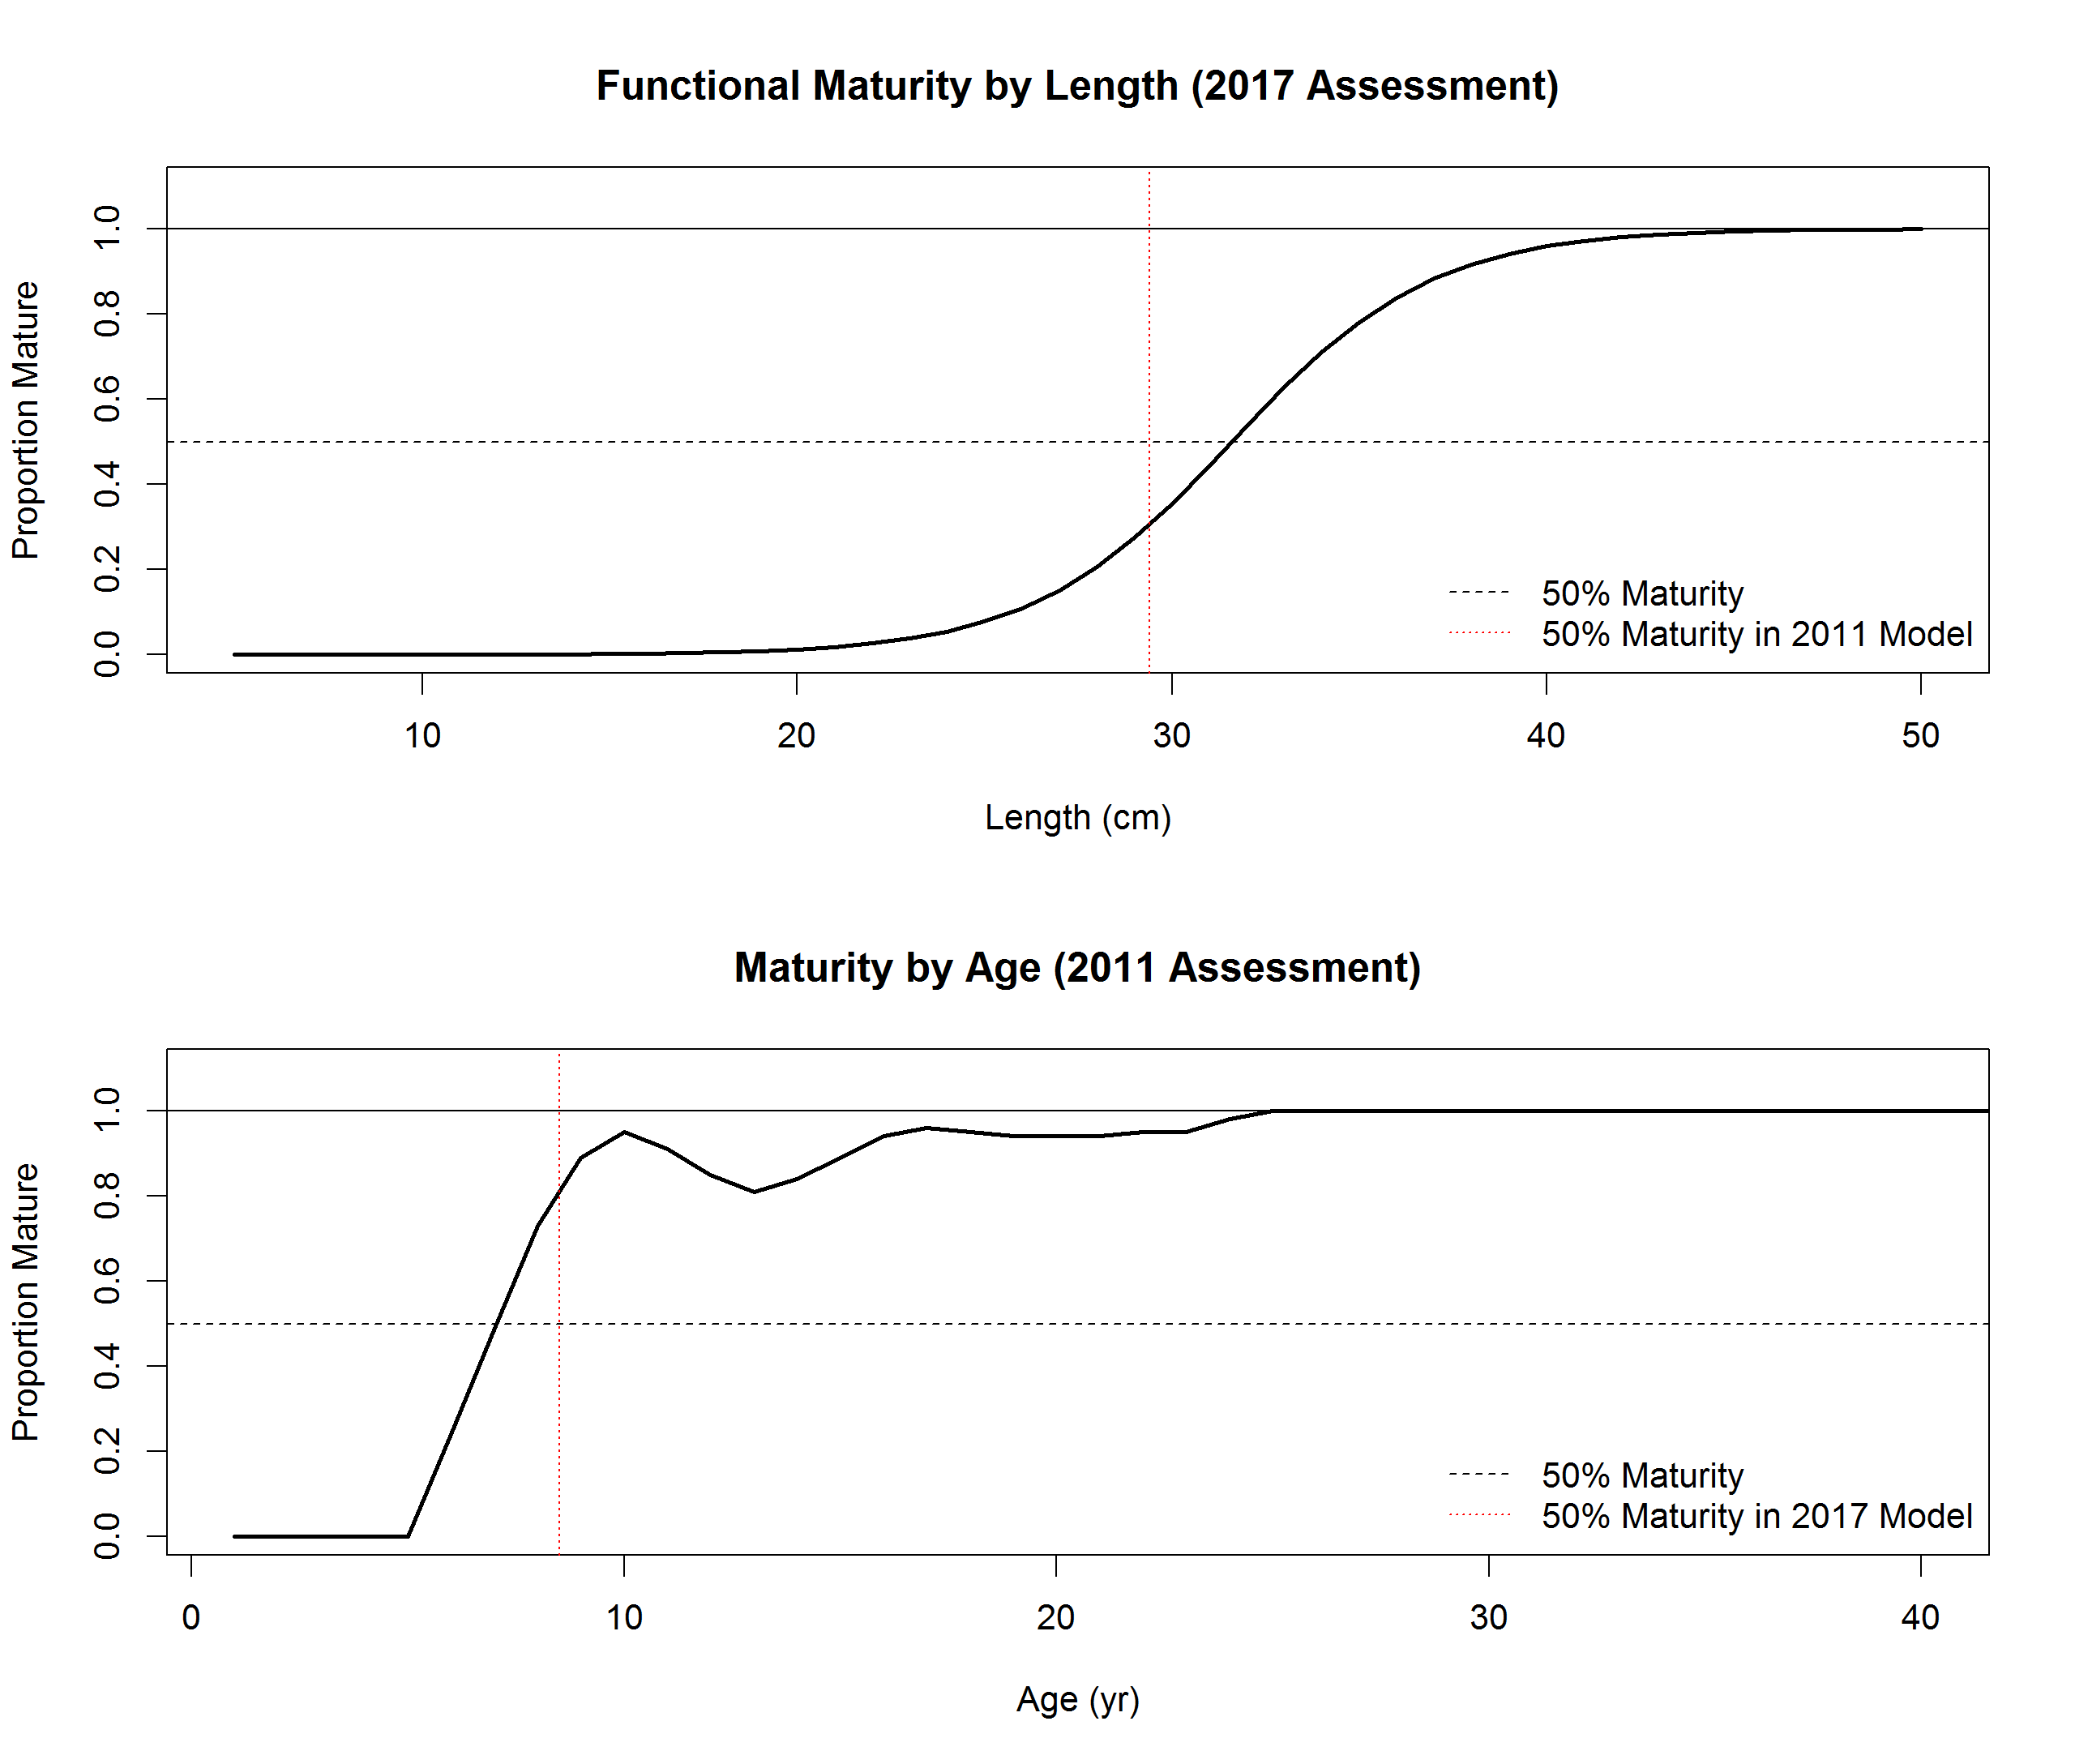
\includegraphics{Figures/Maturity_Comparison.png}
\caption{Comparison between estimated maturity-at-length used in this
assessment and maturity-at-age applied in the 2011 assessment of Pacific
ocean perch. \label{fig:mat_compare}}
\end{figure}

\begin{figure}
\centering
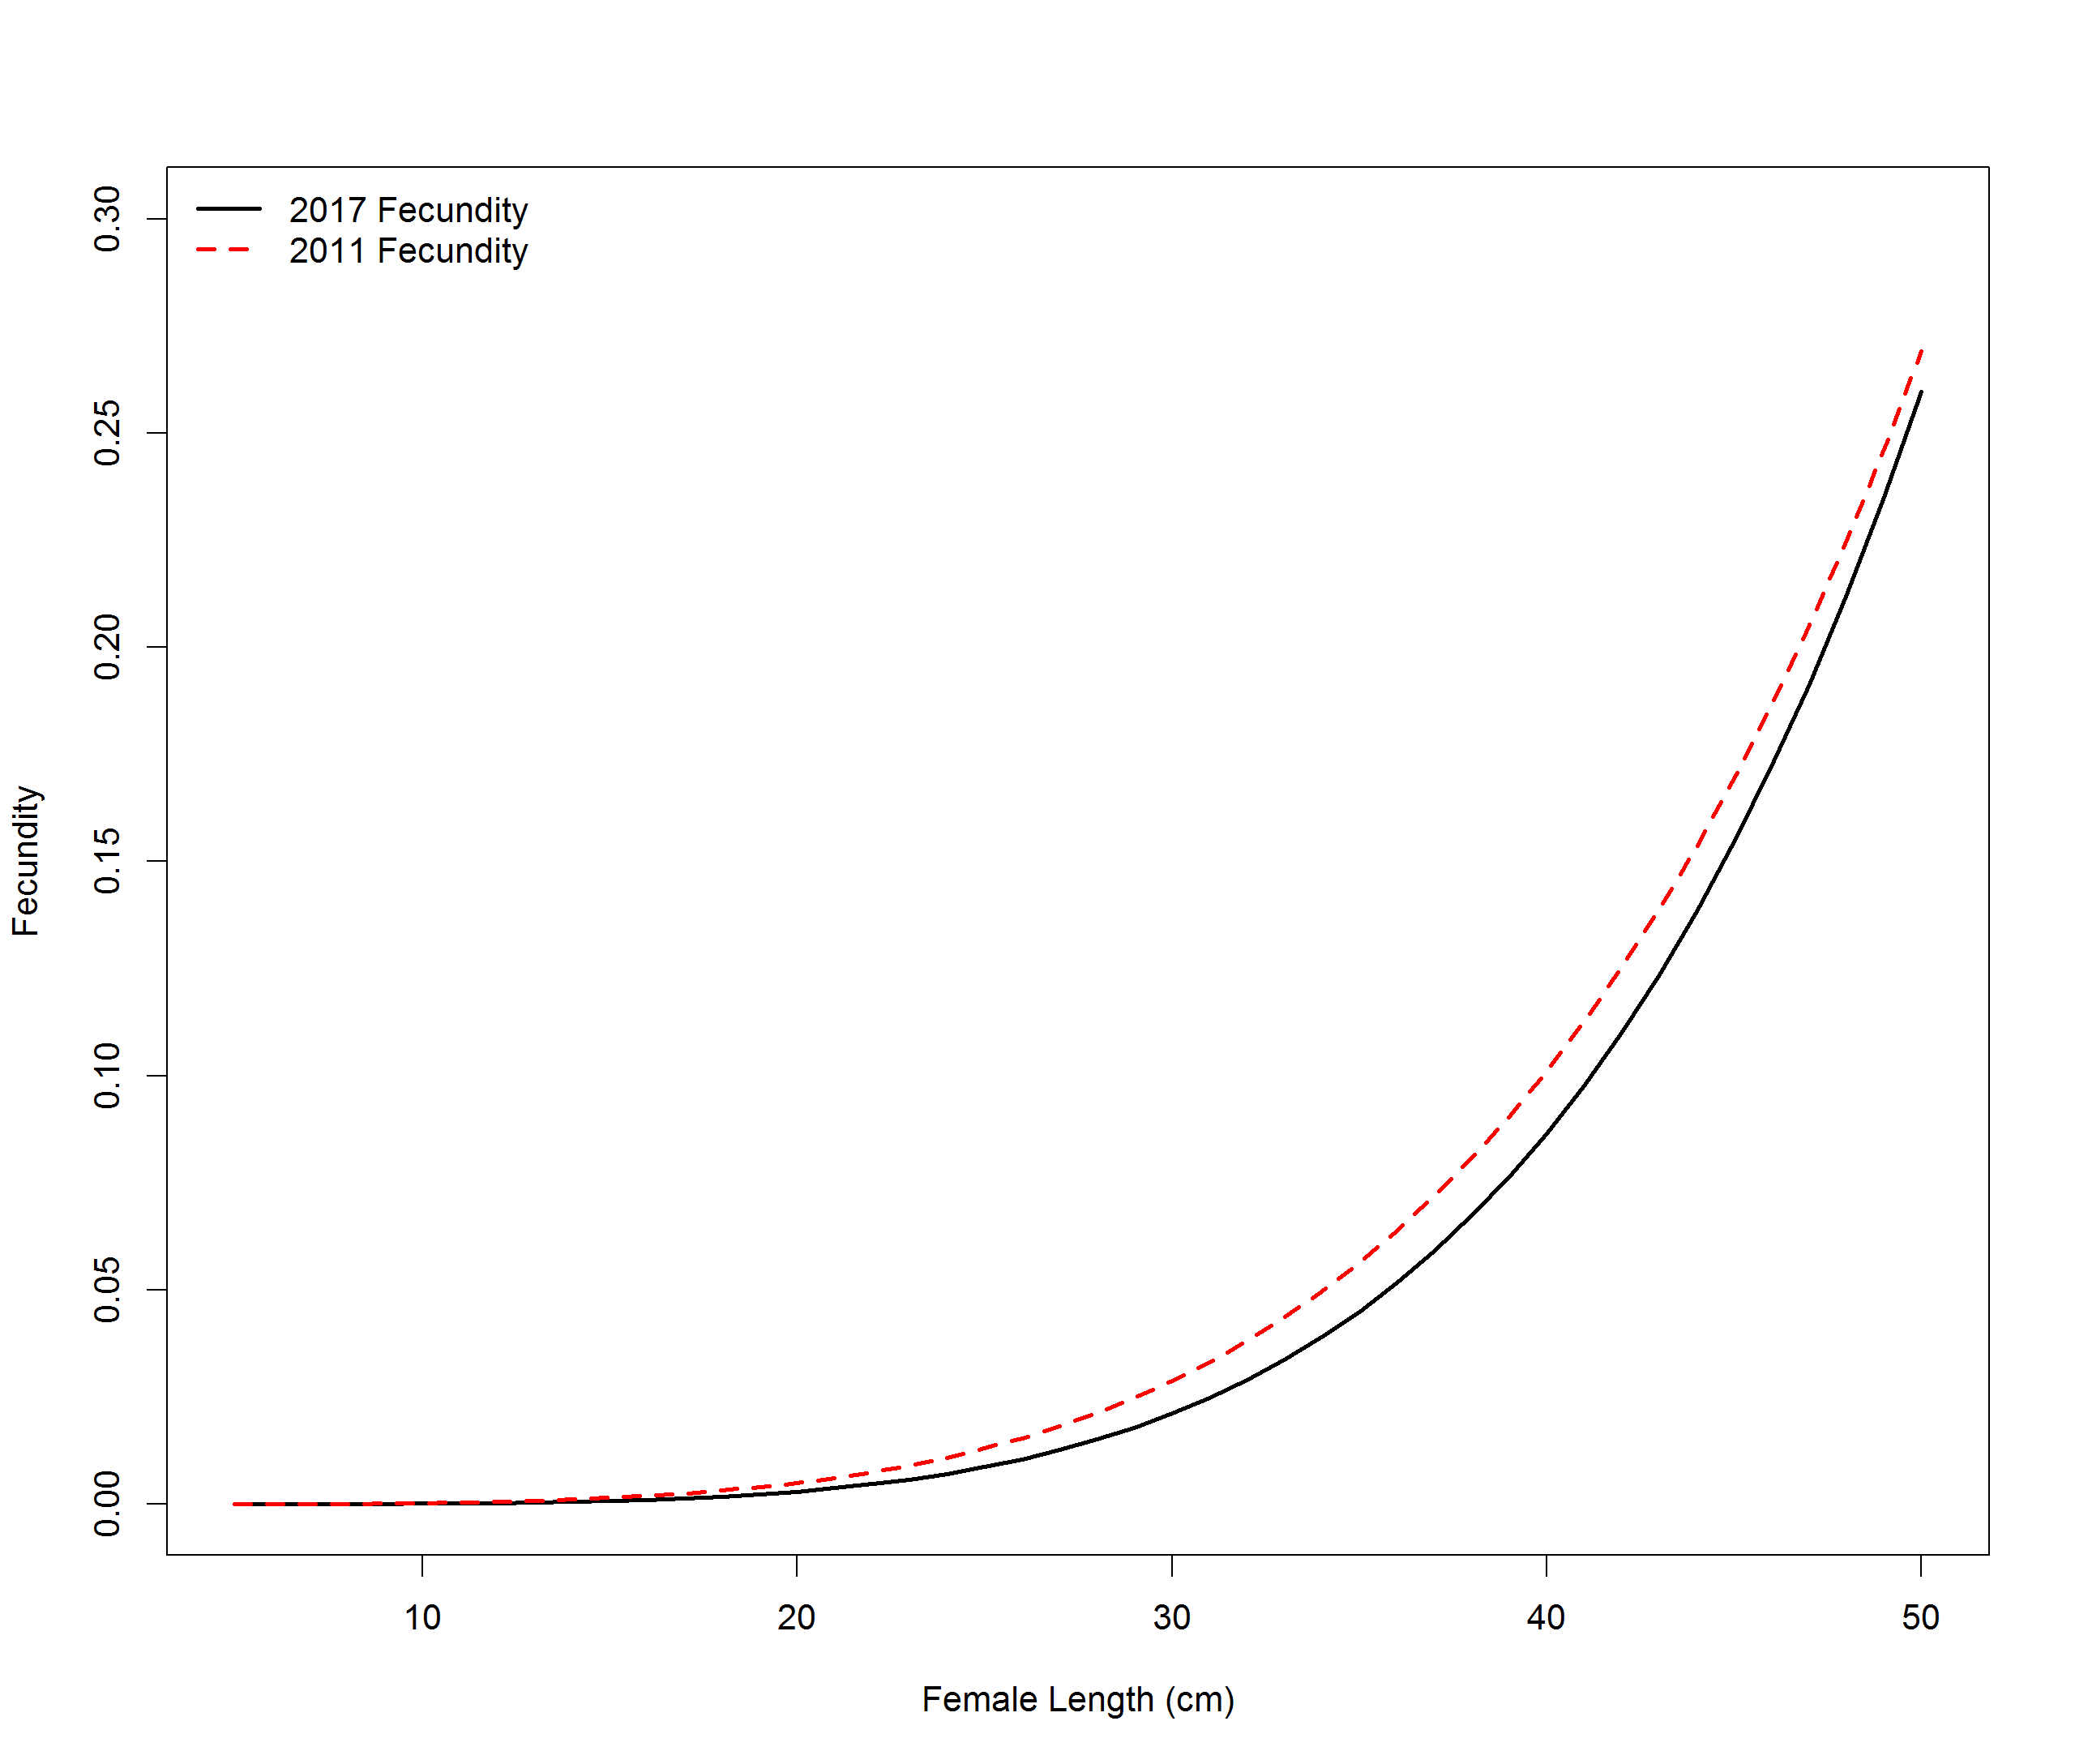
\includegraphics{Figures/Fecundity_Comparison.png}
\caption{Fecundity at length of Pacific ocean perch in the base model
and a comparison of the fecundity in the 2011 assessment.
\label{fig:fecundity}}
\end{figure}

\FloatBarrier 

\begin{figure}
\centering
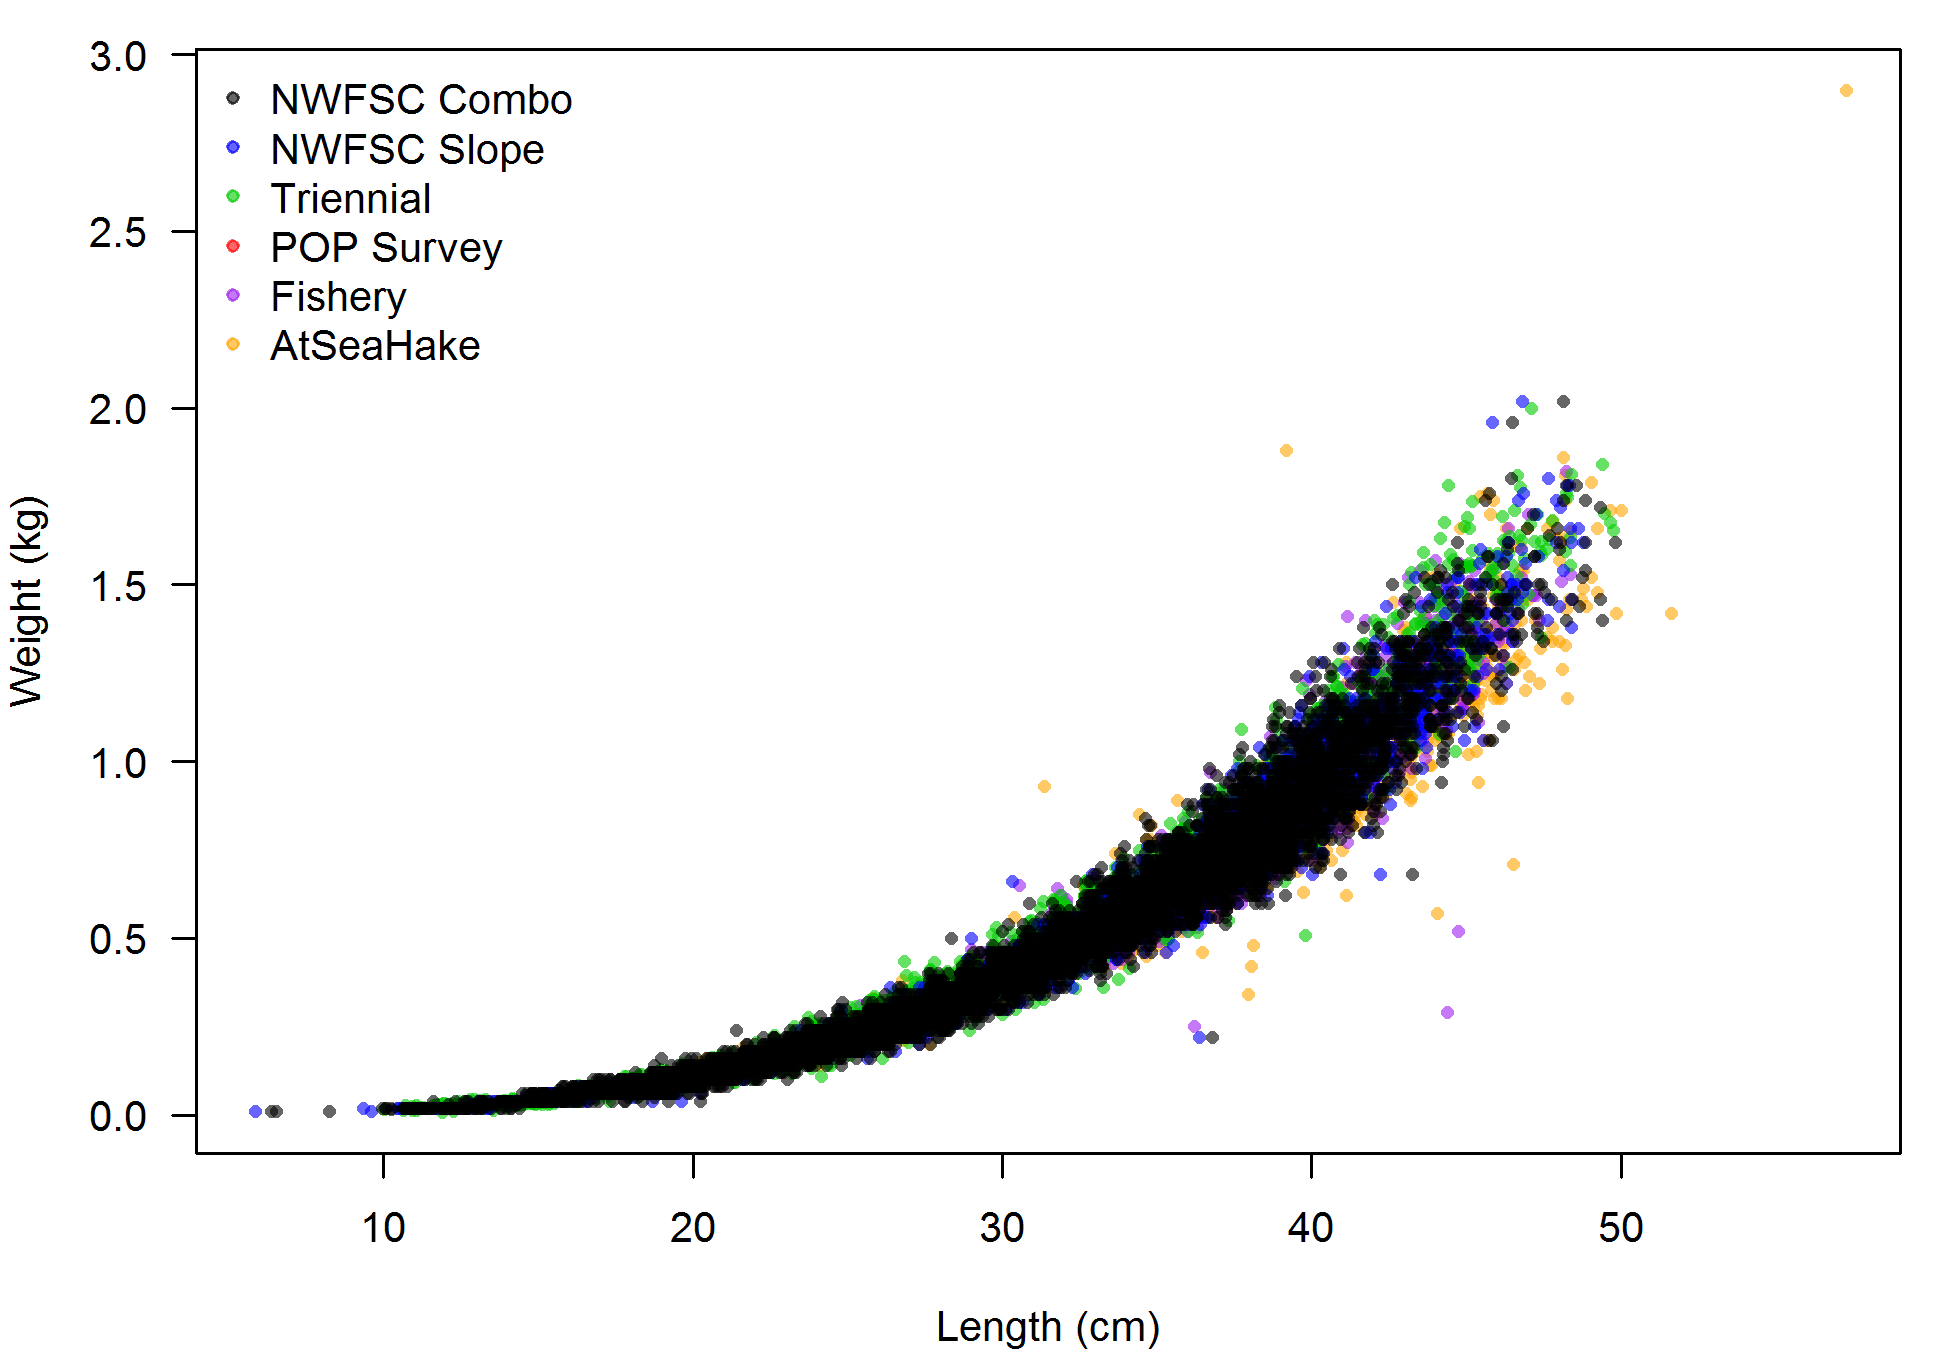
\includegraphics{Figures/weightAtLengthBySource.png}
\caption{Weight-at-length for Pacific ocean perch from all data sources.
\label{fig:Wt_len}}
\end{figure}

\FloatBarrier 

\begin{figure}
\centering
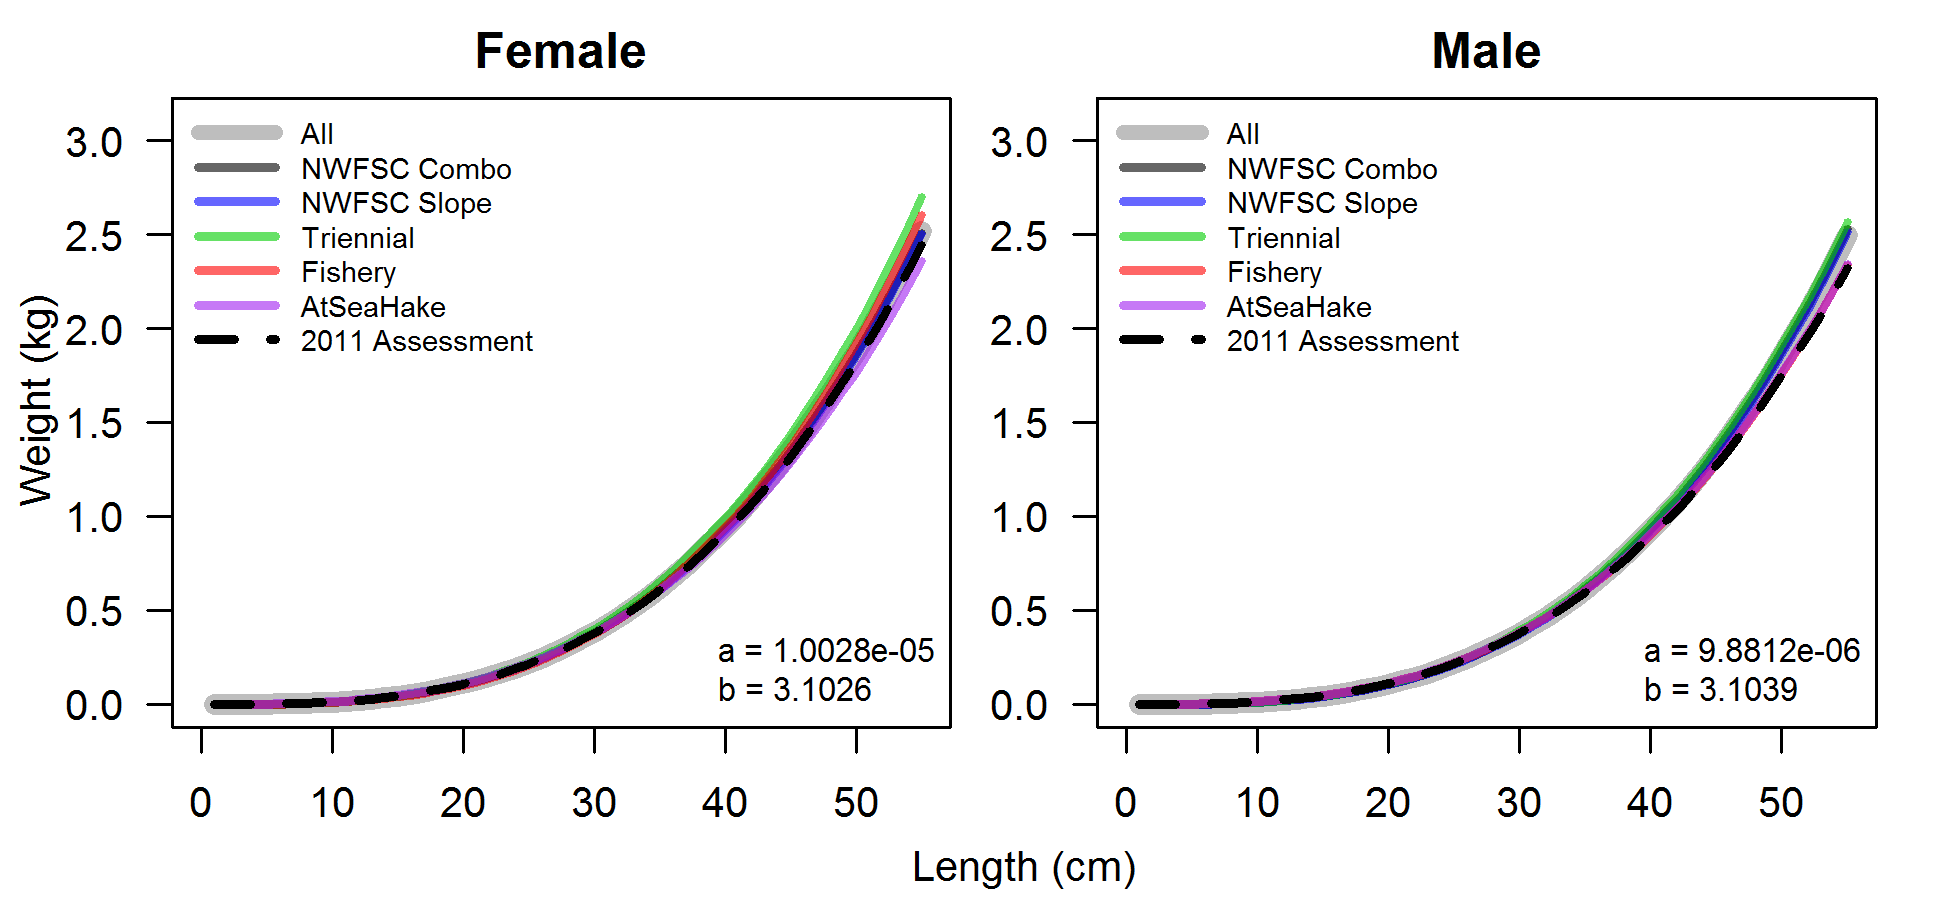
\includegraphics{Figures/weightAtLengthPred.png}
\caption{Estimated weight-at-length for Pacific ocean perch from all
data sources. \label{fig:Wt_len_pred}}
\end{figure}

\FloatBarrier 

\begin{figure}
\centering
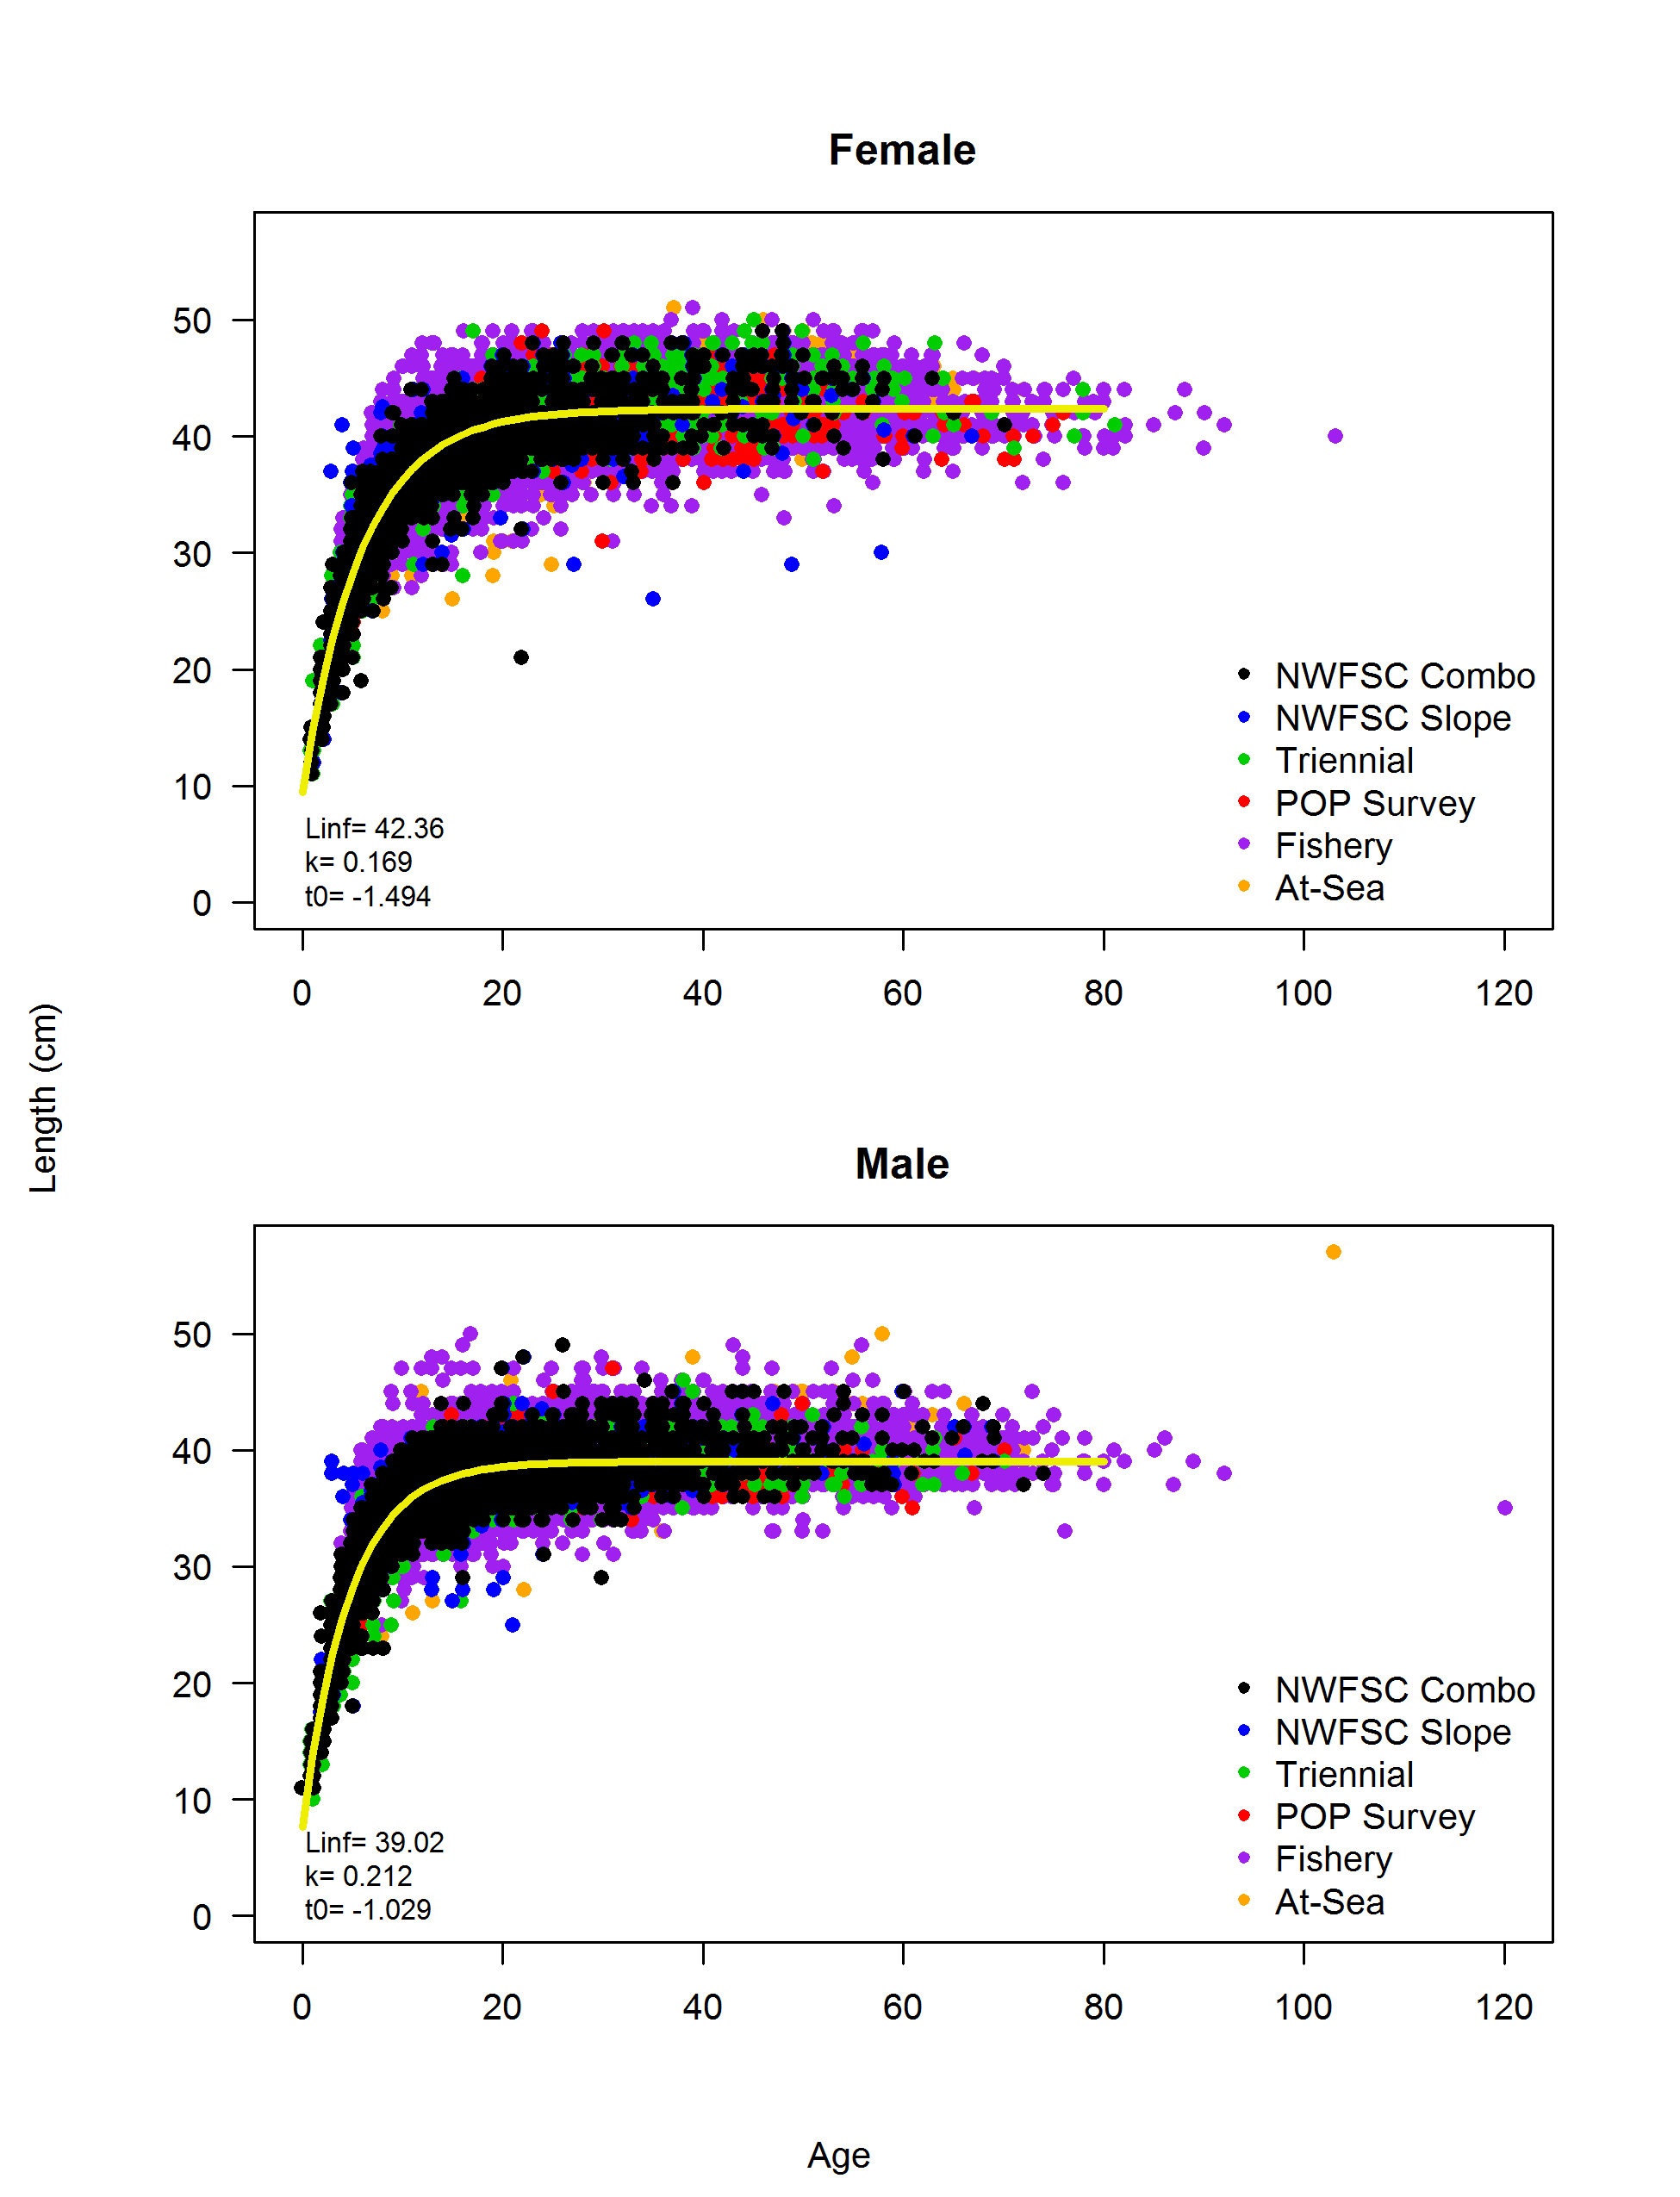
\includegraphics{Figures/LengthAgeAll.png}
\caption{Estimated length-at-age for Pacific ocean perch from all data
sources. \label{fig:Len_Age}}
\end{figure}

\FloatBarrier 

\begin{figure}
\centering
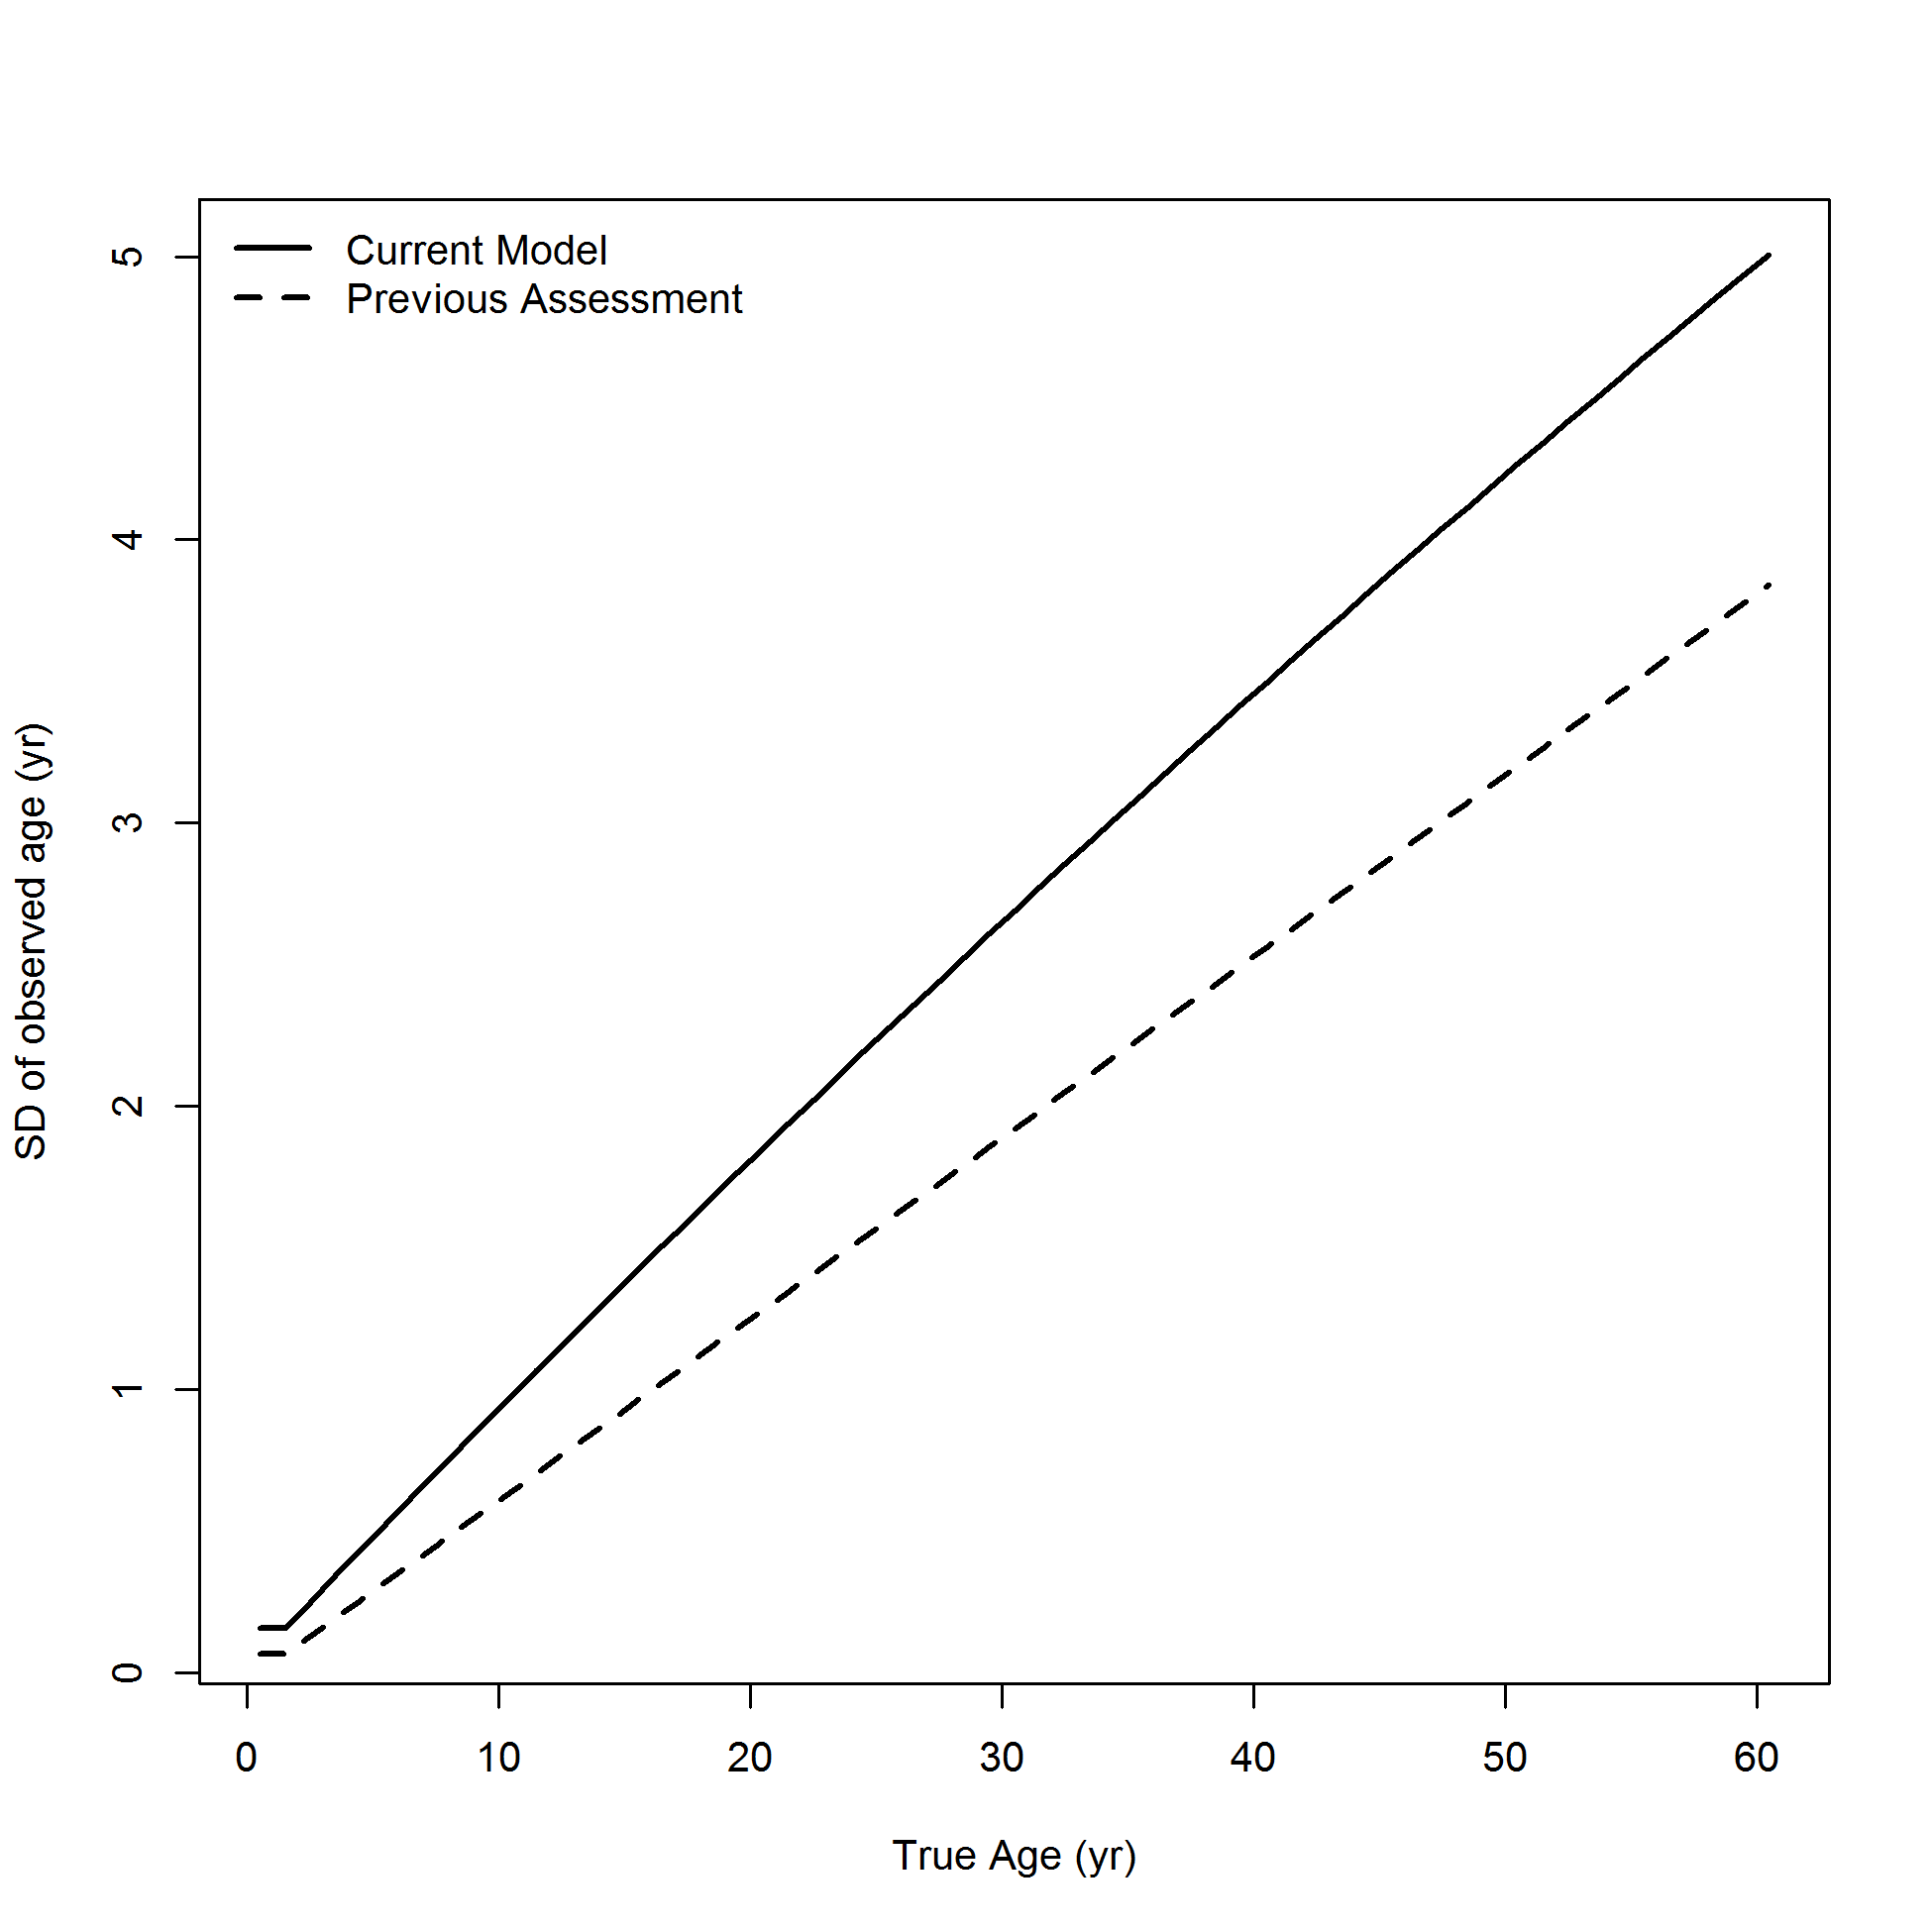
\includegraphics{Figures/Ageing_Error.png}
\caption{The estimated ageing error used in this assessment compared to
the ageing error assumed in the previous assessment for Pacific ocean
perch. \label{fig:Age_Error}}
\end{figure}

\FloatBarrier 

\begin{figure}
\centering
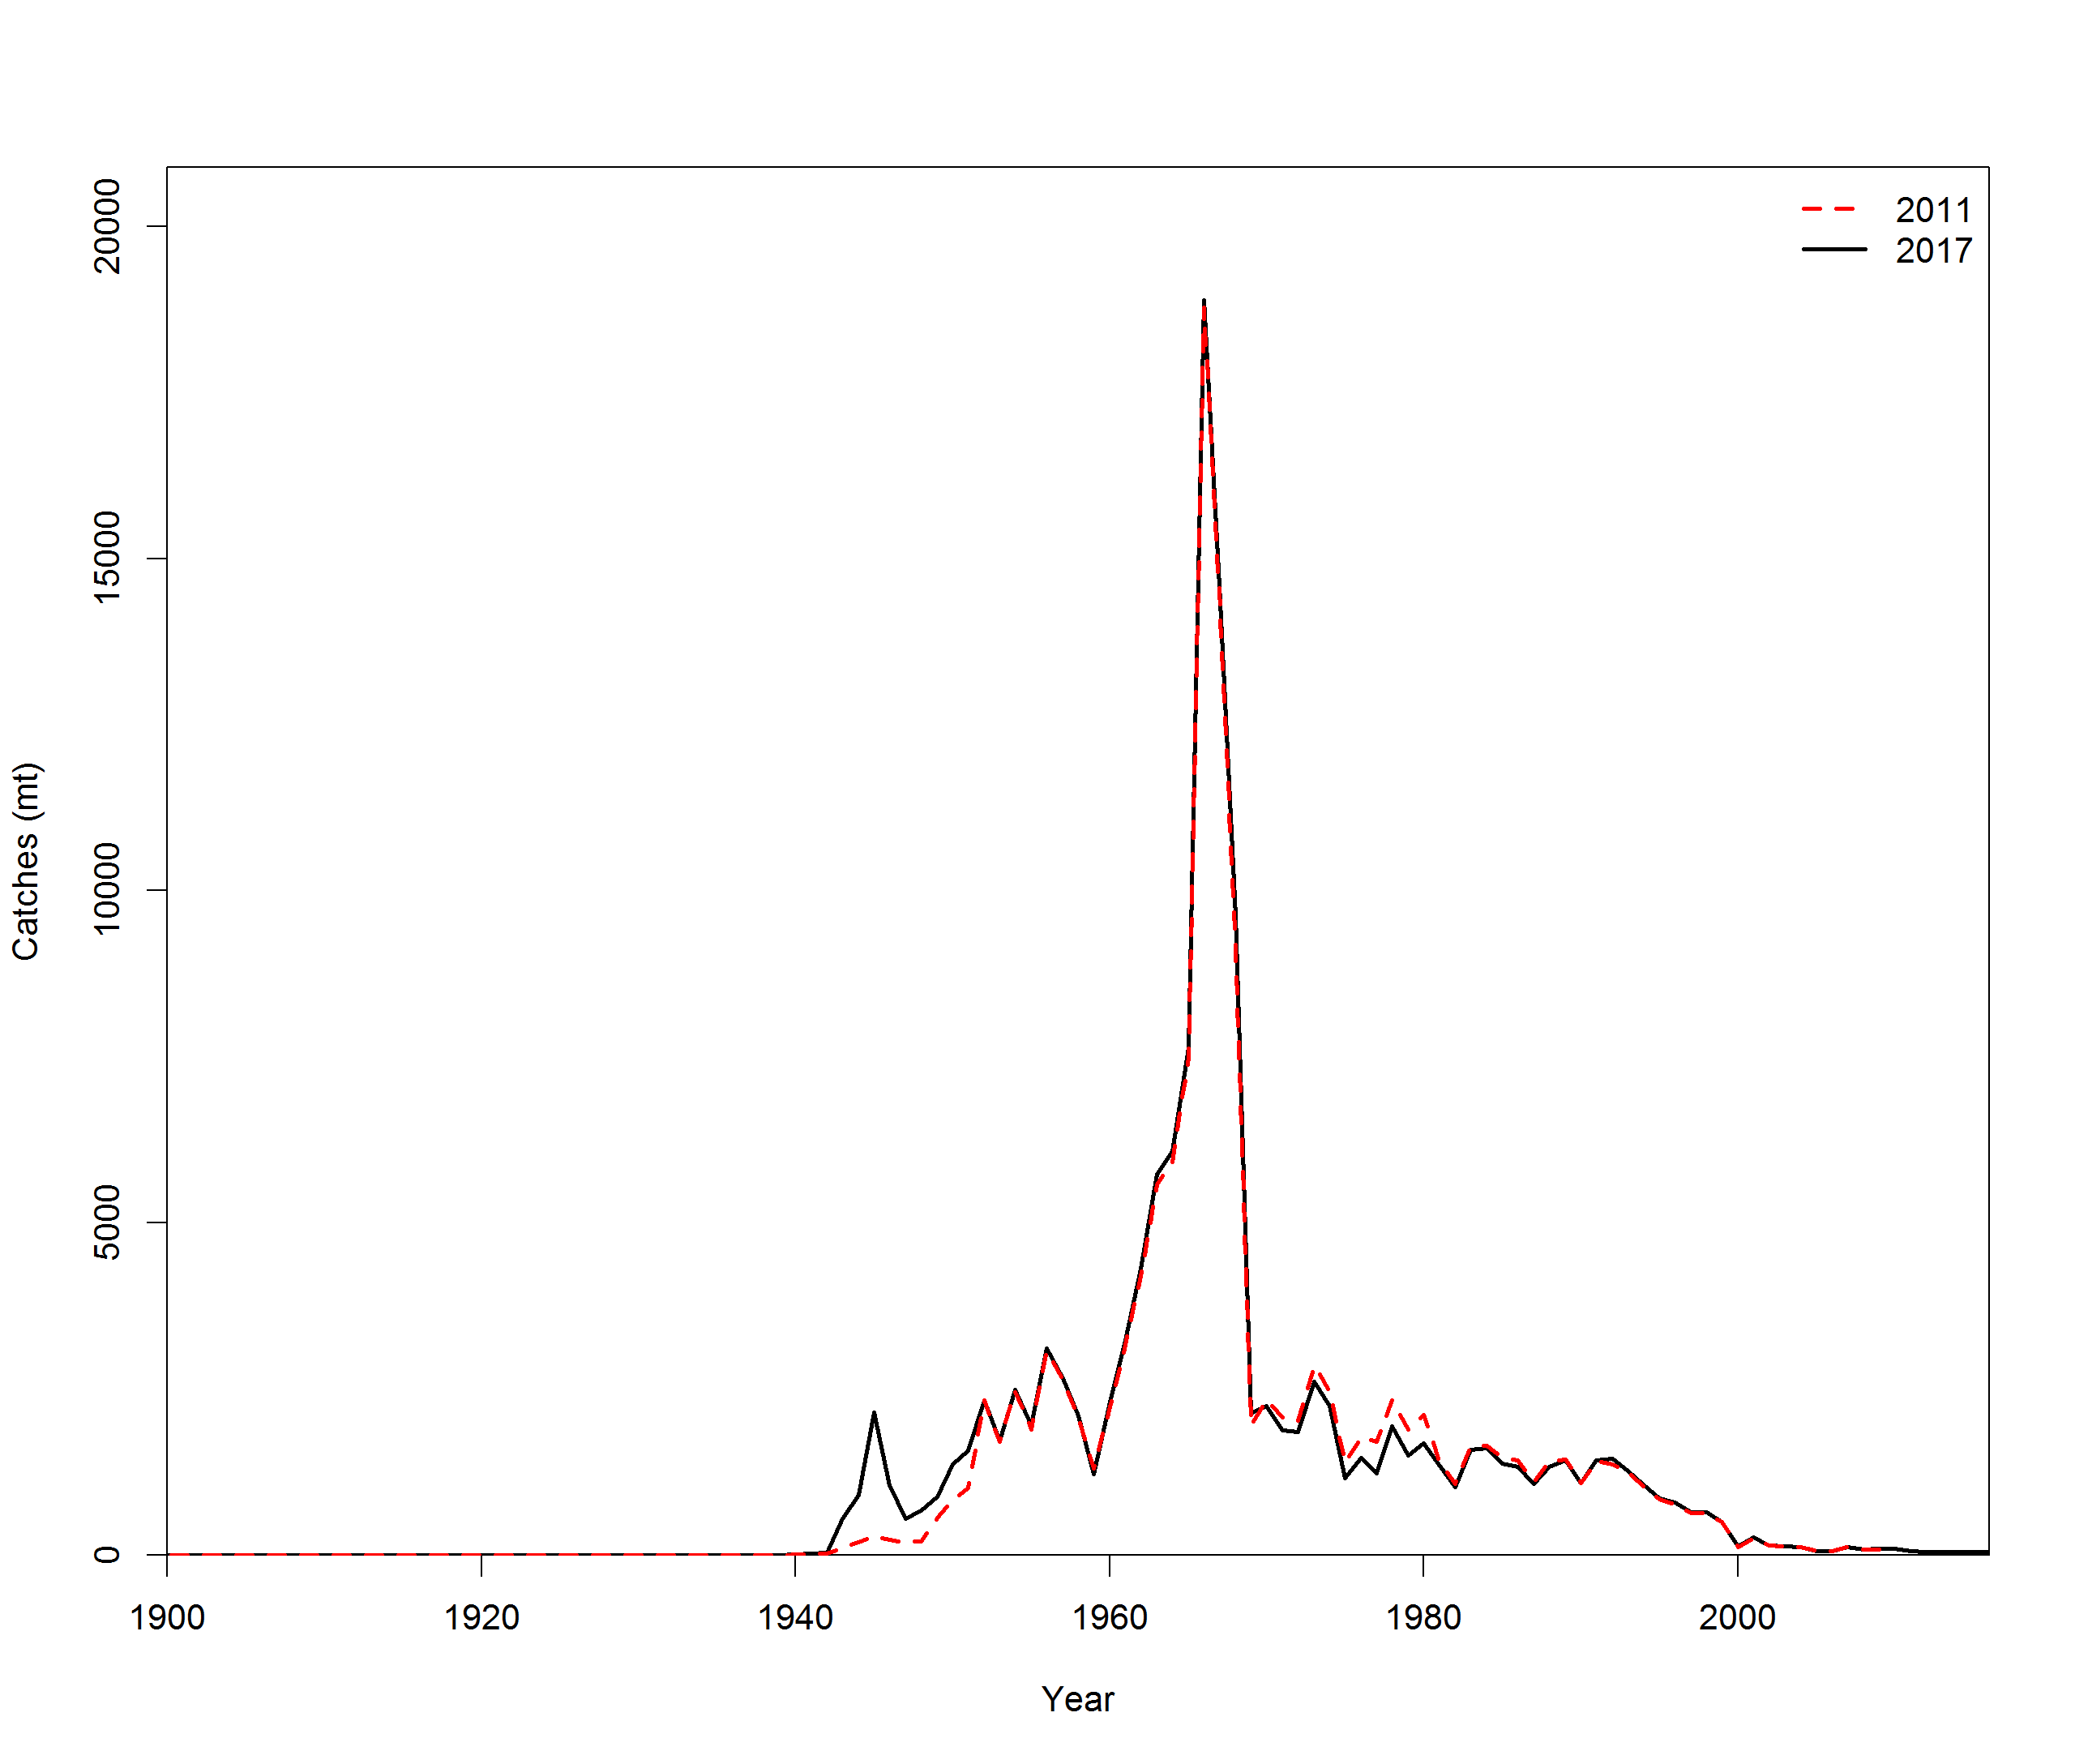
\includegraphics{Figures/Catch_Comparison.png}
\caption{Comparison of the catches assumed by this assessment and the
previous assessment for Pacific ocean perch. \label{fig:Catch_Compare}}
\end{figure}

\FloatBarrier 

\begin{figure}
\centering
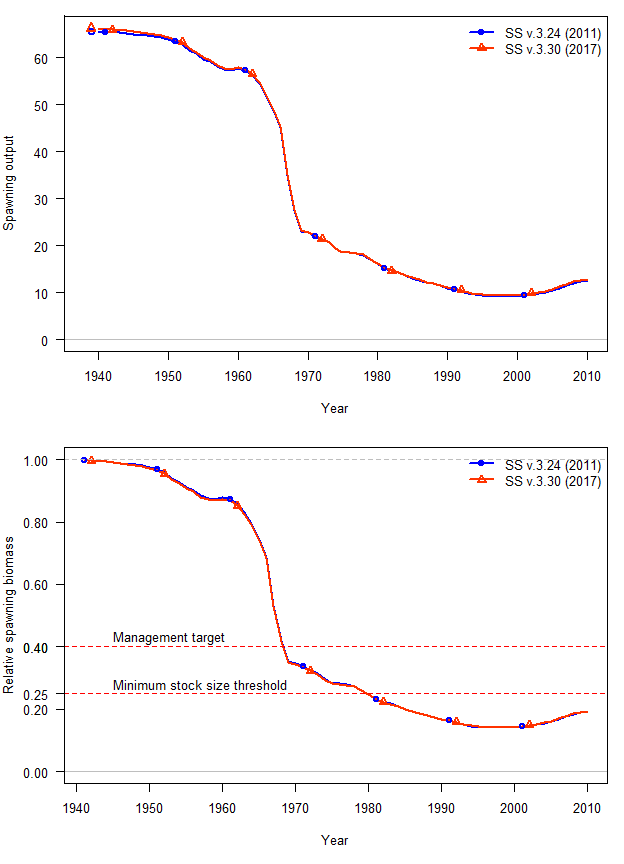
\includegraphics{Figures/bridging.png}
\caption{Comparison of estimates from Stock Synthesis version 3.30 and
3.24 for Pacific ocean perch. \label{fig:bridge}}
\end{figure}

\FloatBarrier 

\begin{figure}
\centering
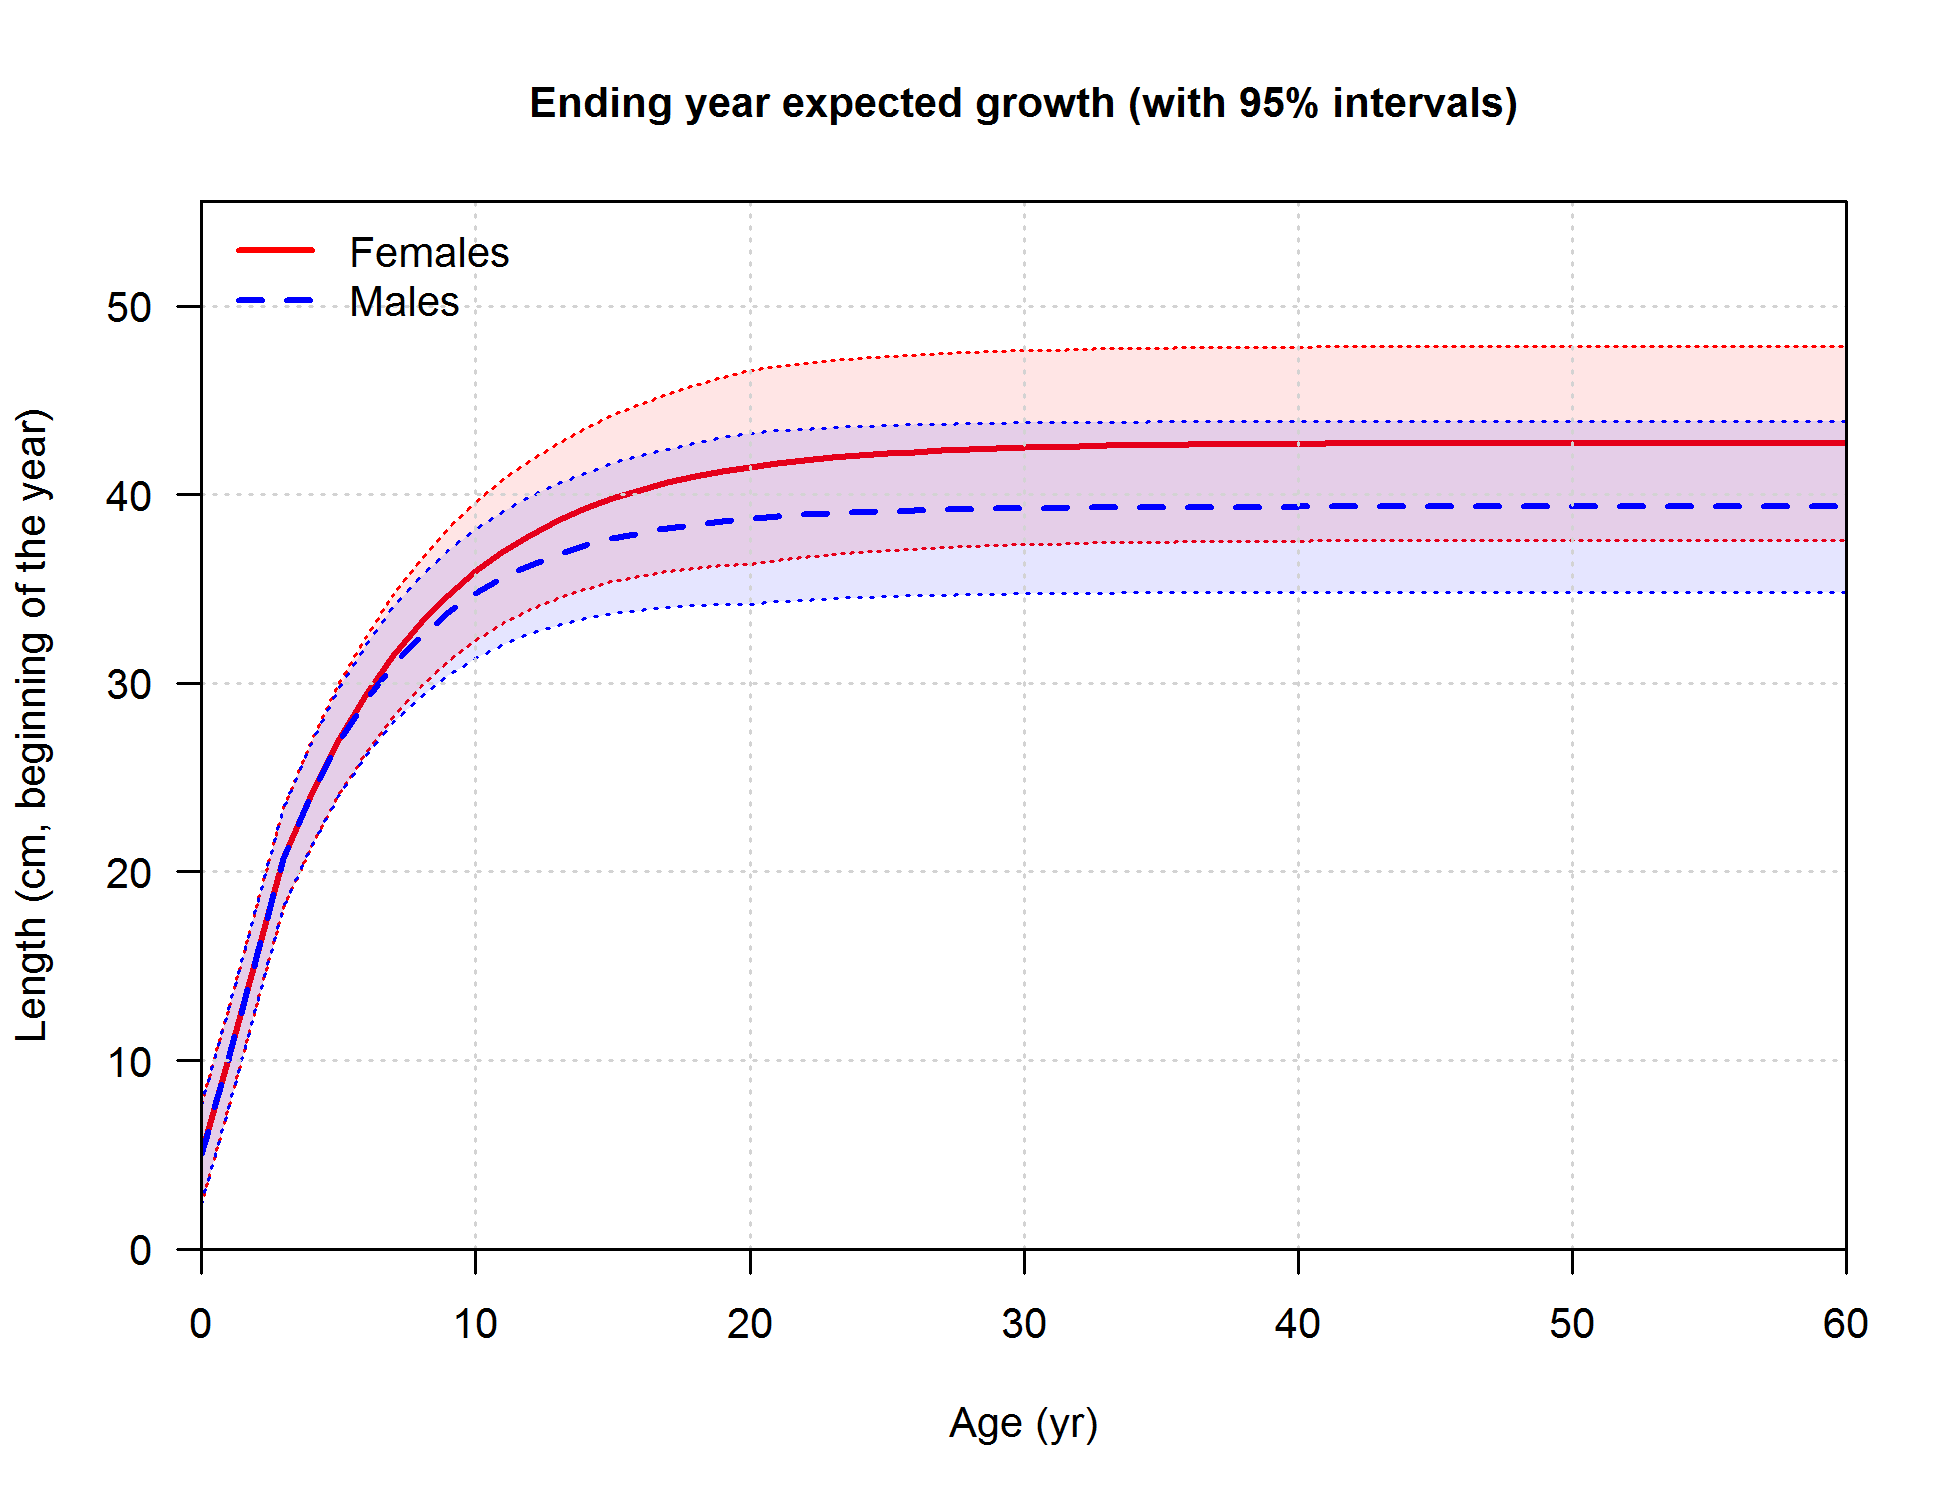
\includegraphics{r4ss/plots_mod1/bio1_sizeatage.png}
\caption{Estimated length-at-age for male and female for Pacific ocean
perch with estimated CV. \label{fig:sizeatage}}
\end{figure}

\FloatBarrier 

\begin{figure}
\centering
\includegraphics{r4ss/plots_mod1/POP_selectivity.png}
\caption{Estimated selectivity by length by each fishery and survey for
Pacific ocean perch. \label{fig:selex}}
\end{figure}

\FloatBarrier 

\begin{figure}
\centering
\includegraphics{r4ss/plots_mod1/POP_retention.png}
\caption{Estimated retention by length by the trawl fishery for Pacific
ocean perch. \label{fig:retention}}
\end{figure}

\FloatBarrier 

\begin{figure}
\centering
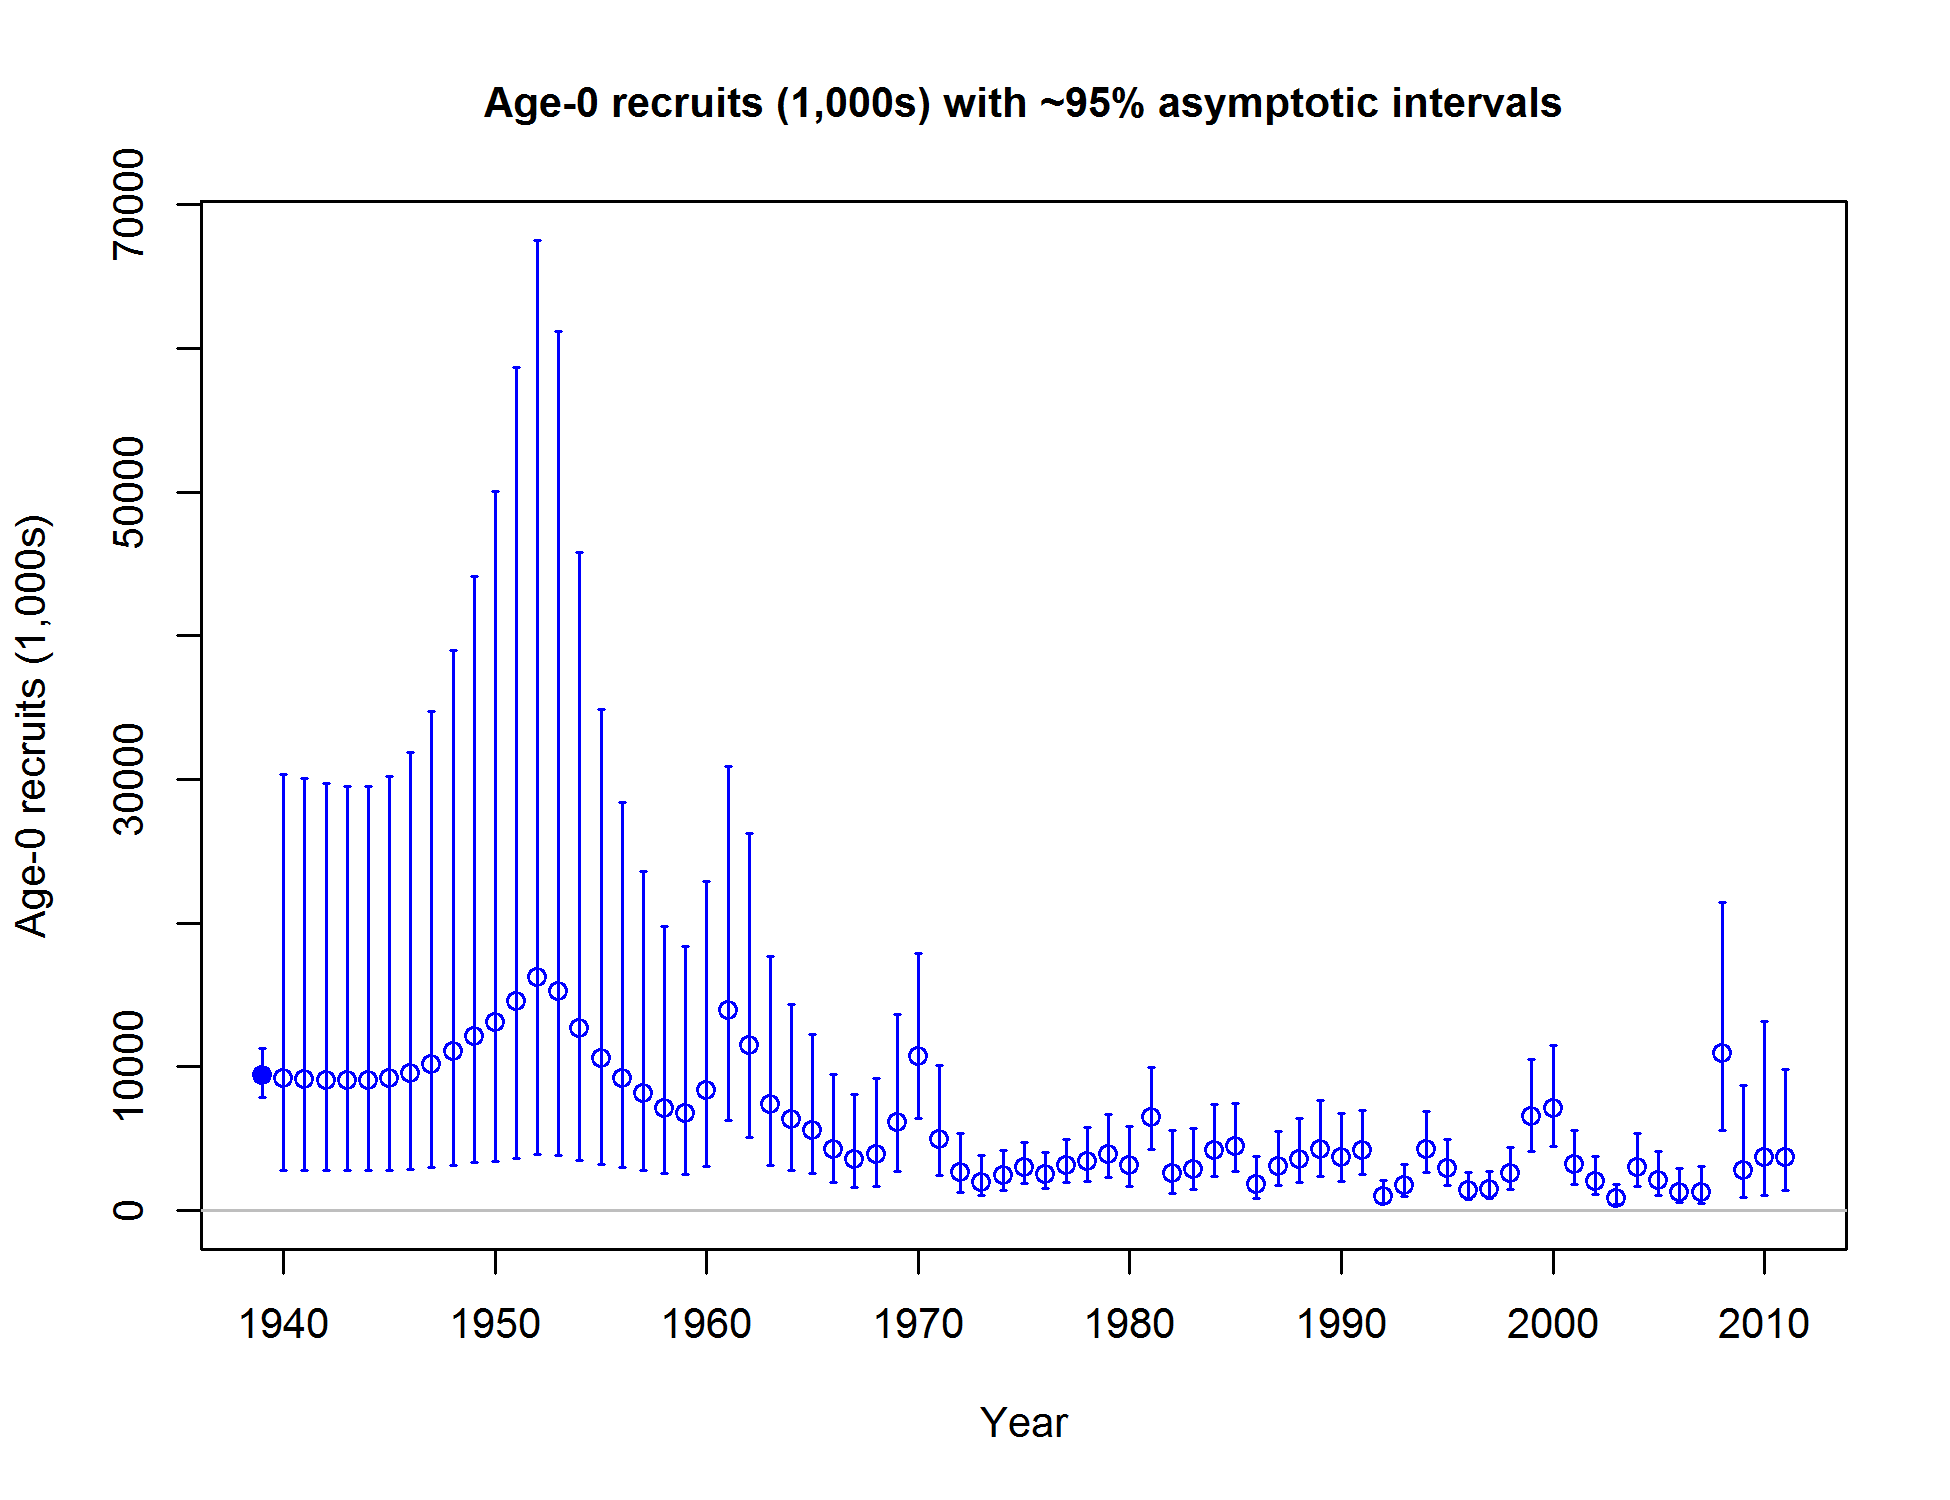
\includegraphics{r4ss/plots_mod1/ts11_Age-0_recruits_(1000s)_with_95_asymptotic_intervals.png}
\caption{Estimated time-series of recruitment for Pacific ocean perch.
\label{fig:recruits}}
\end{figure}

\FloatBarrier

\begin{figure}
\centering
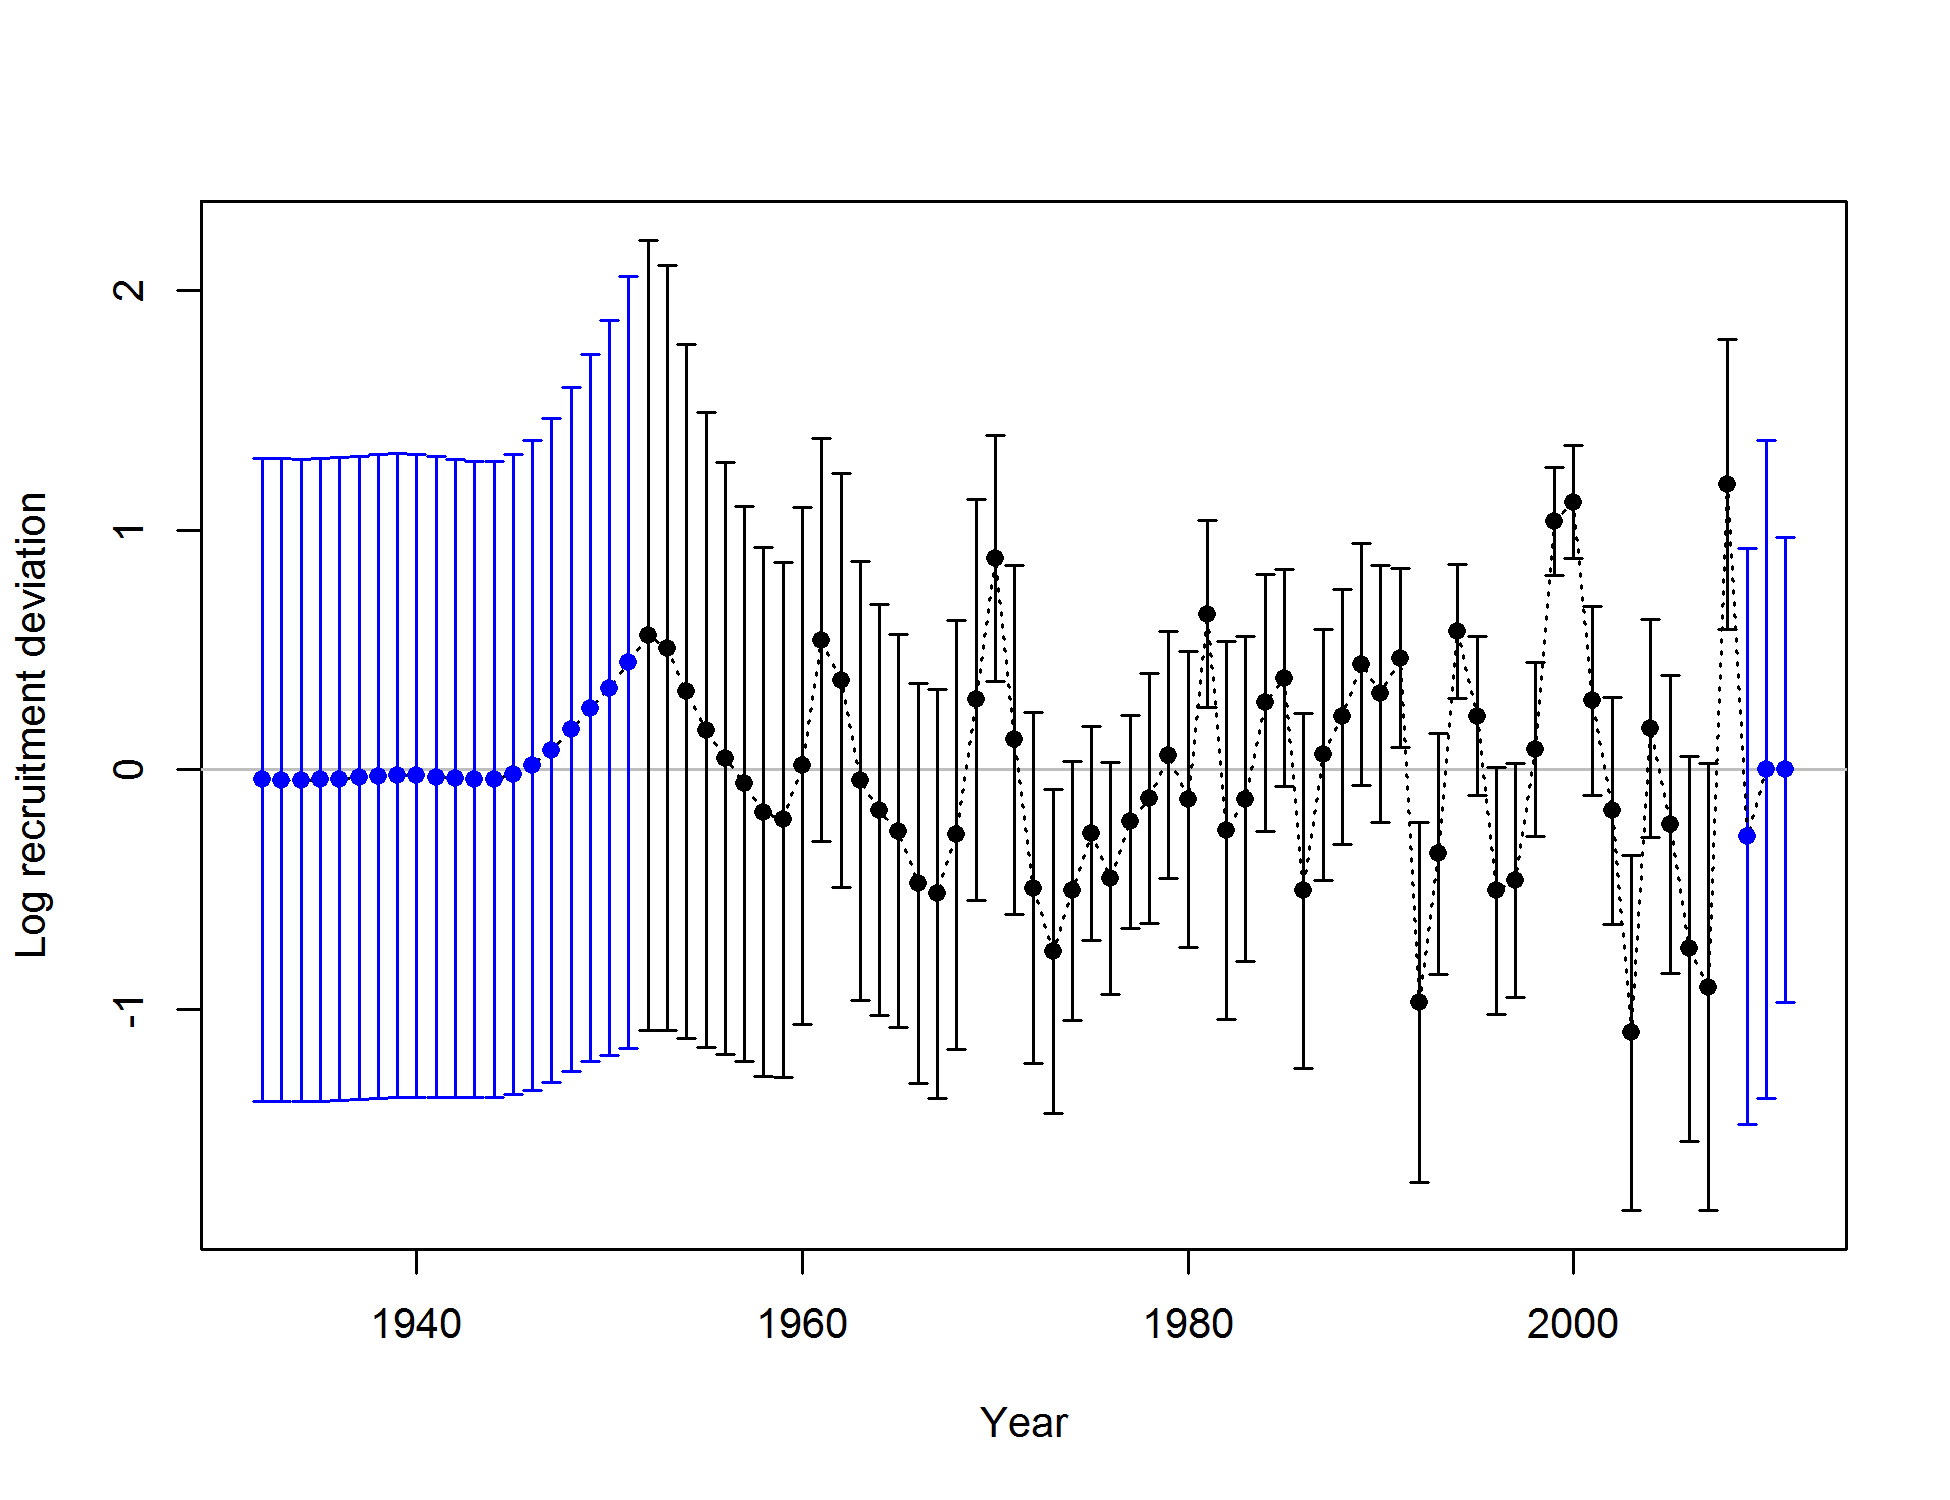
\includegraphics{r4ss/plots_mod1/recdevs2_withbars.png}
\caption{Estimated time-series of recruitment deviations for Pacific
ocean perch. \label{fig:recdevs}}
\end{figure}

\FloatBarrier

\begin{figure}
\centering
\includegraphics{r4ss/plots_mod1/POP_discard_fits.png}
\caption{Estimated fits to the discard rates for Pacific ocean perch.
\label{fig:discard_fits}}
\end{figure}

\FloatBarrier 

\begin{figure}
\centering
\includegraphics{r4ss/plots_mod1/POP_index_fits.png}
\caption{Estimated fits to the CPUE and survey indices for Pacific ocean
perch. \label{fig:index_fits}}
\end{figure}

\FloatBarrier 

\begin{figure}
\centering
\includegraphics{r4ss/plots_mod1/comp_lenfit__aggregated_across_time.png}
\caption{Length compositions aggregated across time by fleet. Labels
`retained' and `discard' indicate retained or discarded samples for each
fleet. Panels without this designation represent the whole catch.
\label{fig:length_agg}}
\end{figure}

\begin{figure}
\centering
\includegraphics{./r4ss/plots_mod1/comp_lenfit_residsflt1mkt1.png}
\caption{Pearson residuals, discard, Fishery (max=3.78)\\
Closed bubbles are positive residuals (observed \textgreater{} expected)
and open bubbles are negative residuals (observed \textless{} expected).
\label{fig:discard_len_pearson}}
\end{figure}

\begin{figure}
\centering
\includegraphics{./r4ss/plots_mod1/comp_lenfit_residsflt1mkt2_page4.png}
\caption{Pearson residuals, retained, Fishery (max=3.2) (plot 4 of 4)\\
Closed bubbles are positive residuals (observed \textgreater{} expected)
and open bubbles are negative residuals (observed \textless{} expected).
\label{fig:fishery_len_pearson}}
\end{figure}

\begin{figure}
\centering
\includegraphics{./r4ss/plots_mod1/comp_lenfit_residsflt2mkt0.png}
\caption{Pearson residuals, whole catch, At\_sea hake (max=2.36)\\
Closed bubbles are positive residuals (observed \textgreater{} expected)
and open bubbles are negative residuals (observed \textless{} expected).
\label{fig:ashop_len_pearson}}
\end{figure}

\begin{figure}
\centering
\includegraphics{./r4ss/plots_mod1/comp_lenfit_residsflt4mkt0.png}
\caption{Pearson residuals, whole catch, Pacific ocean perch survey
(max=1.74)\\
Closed bubbles are positive residuals (observed \textgreater{} expected)
and open bubbles are negative residuals (observed \textless{} expected).
\label{fig:pop_len_pearson}}
\end{figure}

\begin{figure}
\centering
\includegraphics{./r4ss/plots_mod1/comp_lenfit_residsflt5mkt0.png}
\caption{Pearson residuals, whole catch, Triennial survey (max=4.01)\\
Closed bubbles are positive residuals (observed \textgreater{} expected)
and open bubbles are negative residuals (observed \textless{} expected).
\label{fig:tri_len_pearson}}
\end{figure}

\begin{figure}
\centering
\includegraphics{./r4ss/plots_mod1/comp_lenfit_residsflt6mkt0.png}
\caption{Pearson residuals, whole catch, AFSC slope survey (max=2.91)\\
Closed bubbles are positive residuals (observed \textgreater{} expected)
and open bubbles are negative residuals (observed \textless{} expected).
\label{fig:afsc_len_pearson}}
\end{figure}

\begin{figure}
\centering
\includegraphics{./r4ss/plots_mod1/comp_lenfit_residsflt7mkt0.png}
\caption{Pearson residuals, whole catch, NWFSC slope survey (max=3.46)\\
Closed bubbles are positive residuals (observed \textgreater{} expected)
and open bubbles are negative residuals (observed \textless{} expected).
\label{fig:nwfsc_len_pearson}}
\end{figure}

\begin{figure}
\centering
\includegraphics{./r4ss/plots_mod1/comp_lenfit_residsflt8mkt0.png}
\caption{Pearson residuals, whole catch, NWFSC shelf\_slope survey
(max=2.74)\\
Closed bubbles are positive residuals (observed \textgreater{} expected)
and open bubbles are negative residuals (observed \textless{} expected).
\label{fig:nwfsc_combo_len_pearson}}
\end{figure}

\begin{figure}
\centering
\includegraphics{./r4ss/plots_mod1/comp_lenfit_data_weighting_TA1.8_Fishery.png}
\caption{Francis data weighting method TA1.8: Fishery Suggested sample
size adjustment (with 95\% interval) for len data from Fishery: 0.9951
(0.6685\_1.8165) For more info, see Francis, R.I.C.C. (2011). Data
weighting in statistical fisheries stock assessment models. Can. J.
Fish. Aquat. Sci. 68: 1124\_1138. \label{fig:weighting_len_fishery}}
\end{figure}

\begin{figure}
\centering
\includegraphics{./r4ss/plots_mod1/comp_lenfit_data_weighting_TA1.8_At-sea hake.png}
\caption{Francis data weighting method TA1.8: At\_sea hake Suggested
sample size adjustment (with 95\% interval) for len data from At\_sea
hake: 1.0115 (0.5352\_4.8582) For more info, see Francis, R.I.C.C.
(2011). Data weighting in statistical fisheries stock assessment models.
Can. J. Fish. Aquat. Sci. 68: 1124\_1138.
\label{fig:weighting_len_ashop}}
\end{figure}

\begin{figure}
\centering
\includegraphics{./r4ss/plots_mod1/comp_lenfit_data_weighting_TA1.8_Pacific ocean perch survey.png}
\caption{Francis data weighting method TA1.8: Pacific ocean perch survey
Suggested sample size adjustment (with 95\% interval) for len data from
Pacific ocean perch survey: 6.7496 (6.7496\_Inf) For more info, see
Francis, R.I.C.C. (2011). Data weighting in statistical fisheries stock
assessment models. Can. J. Fish. Aquat. Sci. 68: 1124\_1138.
\label{fig:weighting_len_pop}}
\end{figure}

\begin{figure}
\centering
\includegraphics{./r4ss/plots_mod1/comp_lenfit_data_weighting_TA1.8_Triennial survey.png}
\caption{Francis data weighting method TA1.8: Triennial survey Suggested
sample size adjustment (with 95\% interval) for len data from Triennial
survey: 1.0004 (0.5362\_5.786) For more info, see Francis, R.I.C.C.
(2011). Data weighting in statistical fisheries stock assessment models.
Can. J. Fish. Aquat. Sci. 68: 1124\_1138.
\label{fig:weighting_len_triennial}}
\end{figure}

\begin{figure}
\centering
\includegraphics{./r4ss/plots_mod1/comp_lenfit_data_weighting_TA1.8_AFSC slope survey.png}
\caption{Francis data weighting method TA1.8: AFSC slope survey
Suggested sample size adjustment (with 95\% interval) for len data from
AFSC slope survey: 1.0151 (0.5859\_16.7225) For more info, see Francis,
R.I.C.C. (2011). Data weighting in statistical fisheries stock
assessment models. Can. J. Fish. Aquat. Sci. 68: 1124\_1138.
\label{fig:weighting_len_afsc}}
\end{figure}

\begin{figure}
\centering
\includegraphics{./r4ss/plots_mod1/comp_lenfit_data_weighting_TA1.8_NWFSC slope survey.png}
\caption{Francis data weighting method TA1.8: NWFSC slope survey
Suggested sample size adjustment (with 95\% interval) for len data from
NWFSC slope survey: 0.9922 (0.9922\_Inf) For more info, see Francis,
R.I.C.C. (2011). Data weighting in statistical fisheries stock
assessment models. Can. J. Fish. Aquat. Sci. 68: 1124\_1138.
\label{fig:weighting_len_nwfs}}
\end{figure}

\begin{figure}
\centering
\includegraphics{./r4ss/plots_mod1/comp_lenfit_data_weighting_TA1.8_NWFSC shelf-slope survey.png}
\caption{Francis data weighting method TA1.8: NWFSC shelf\_slope survey
Suggested sample size adjustment (with 95\% interval) for len data from
NWFSC shelf\_slope survey: 1.0055 (0.6199\_4.021) For more info, see
Francis, R.I.C.C. (2011). Data weighting in statistical fisheries stock
assessment models. Can. J. Fish. Aquat. Sci. 68: 1124\_1138.
\label{fig:weighting_len_nwfsccombo}}
\end{figure}

\FloatBarrier

\begin{figure}
\centering
\includegraphics{r4ss/plots_mod1/comp_lenfit__aggregated_across_time.png}
\caption{Age compositions aggregated across time by fleet.
\label{fig:length_agg}}
\end{figure}

\begin{figure}
\centering
\includegraphics{./r4ss/plots_mod1/comp_agefit_residsflt1mkt2_page2.png}
\caption{Pearson residuals, retained, Fishery (max=5.4) (plot 2 of 2)\\
Closed bubbles are positive residuals (observed \textgreater{} expected)
and open bubbles are negative residuals (observed \textless{} expected).
\label{fig:fishery_age_pearson}}
\end{figure}

\begin{figure}
\centering
\includegraphics{./r4ss/plots_mod1/comp_agefit_residsflt2mkt0.png}
\caption{Pearson residuals, whole catch, At\_sea hake (max=4.08)\\
Closed bubbles are positive residuals (observed \textgreater{} expected)
and open bubbles are negative residuals (observed \textless{} expected).
\label{fig:ashop_age_pearson}}
\end{figure}

\begin{figure}
\centering
\includegraphics{./r4ss/plots_mod1/comp_agefit_residsflt4mkt0.png}
\caption{Pearson residuals, whole catch, Pacific ocean perch survey
(max=2.76)\\
Closed bubbles are positive residuals (observed \textgreater{} expected)
and open bubbles are negative residuals (observed \textless{} expected).
\label{fig:pop_age_pearson}}
\end{figure}

\begin{figure}
\centering
\includegraphics{./r4ss/plots_mod1/comp_agefit_residsflt5mkt0.png}
\caption{Pearson residuals, whole catch, Triennial survey (max=3.75)\\
Closed bubbles are positive residuals (observed \textgreater{} expected)
and open bubbles are negative residuals (observed \textless{} expected).
\label{fig:tri_age_pearson}}
\end{figure}

\begin{figure}
\centering
\includegraphics{./r4ss/plots_mod1/comp_agefit_residsflt7mkt0.png}
\caption{Pearson residuals, whole catch, NWFSC slope survey (max=2.34)\\
Closed bubbles are positive residuals (observed \textgreater{} expected)
and open bubbles are negative residuals (observed \textless{} expected).
\label{fig:nwfsc__pearson}}
\end{figure}

\begin{figure}
\centering
\includegraphics{./r4ss/plots_mod1/comp_condAALfit_residsflt8mkt0_page1.png}
\caption{Pearson residuals, whole catch, NWFSC shelf\_slope survey
(max=18.49) (plot 1 of 2) \label{fig:nwsfc_combo_age_aal1}}
\end{figure}

\begin{figure}
\centering
\includegraphics{./r4ss/plots_mod1/comp_condAALfit_residsflt8mkt0_page2.png}
\caption{Pearson residuals, whole catch, NWFSC shelf\_slope survey
(max=18.49) (plot 1 of 2) (plot 2 of 2)
\label{fig:nwsfc_combo_age_aal2}}
\end{figure}

\begin{figure}
\centering
\includegraphics{./r4ss/plots_mod1/comp_condAALfit_Andre_plotsflt8mkt0_page1.png}
\caption{Conditional AAL plot, whole catch, NWFSC shelf\_slope survey
(plot 1 of 5) These plots show mean age and std. dev. in conditional
AAL. Left plots are mean AAL by size\_class (obs. and pred.) with 90\%
CIs based on adding 1.64 SE of mean to the data. Right plots in each
pair are SE of mean AAL (obs. and pred.) with 90\% CIs based on the
chi\_square distribution. \label{fig:nwfsc_combo_andre_1}}
\end{figure}

\begin{figure}
\centering
\includegraphics{./r4ss/plots_mod1/comp_condAALfit_Andre_plotsflt8mkt0_page2.png}
\caption{Conditional AAL plot, whole catch, NWFSC shelf\_slope survey
(plot 2 of 5) These plots show mean age and std. dev. in conditional
AAL. Left plots are mean AAL by size\_class (obs. and pred.) with 90\%
CIs based on adding 1.64 SE of mean to the data. Right plots in each
pair are SE of mean AAL (obs. and pred.) with 90\% CIs based on the
chi\_square distribution. \label{fig:nwfsc_combo_andre_2}}
\end{figure}

\begin{figure}
\centering
\includegraphics{./r4ss/plots_mod1/comp_condAALfit_Andre_plotsflt8mkt0_page3.png}
\caption{Conditional AAL plot, whole catch, NWFSC shelf\_slope survey
(plot 3 of 5) These plots show mean age and std. dev. in conditional
AAL. Left plots are mean AAL by size\_class (obs. and pred.) with 90\%
CIs based on adding 1.64 SE of mean to the data. Right plots in each
pair are SE of mean AAL (obs. and pred.) with 90\% CIs based on the
chi\_square distribution. \label{fig:nwfsc_combo_andre_3}}
\end{figure}

\begin{figure}
\centering
\includegraphics{./r4ss/plots_mod1/comp_condAALfit_Andre_plotsflt8mkt0_page4.png}
\caption{Conditional AAL plot, whole catch, NWFSC shelf\_slope survey
(plot 4 of 5) These plots show mean age and std. dev. in conditional
AAL. Left plots are mean AAL by size\_class (obs. and pred.) with 90\%
CIs based on adding 1.64 SE of mean to the data. Right plots in each
pair are SE of mean AAL (obs. and pred.) with 90\% CIs based on the
chi\_square distribution. \label{fig:nwfsc_combo_andre_4}}
\end{figure}

\begin{figure}
\centering
\includegraphics{./r4ss/plots_mod1/comp_condAALfit_Andre_plotsflt8mkt0_page5.png}
\caption{Conditional AAL plot, whole catch, NWFSC shelf\_slope survey
(plot 5 of 5) These plots show mean age and std. dev. in conditional
AAL. Left plots are mean AAL by size\_class (obs. and pred.) with 90\%
CIs based on adding 1.64 SE of mean to the data. Right plots in each
pair are SE of mean AAL (obs. and pred.) with 90\% CIs based on the
chi\_square distribution. \label{fig:nwfsc_combo_andre_5}}
\end{figure}

\begin{figure}
\centering
\includegraphics{./r4ss/plots_mod1/comp_agefit_data_weighting_TA1.8_Fishery.png}
\caption{Francis data weighting method TA1.8: Fishery Suggested sample
size adjustment (with 95\% interval) for age data from Fishery: 0.9921
(0.6365\_1.9959) For more info, see Francis, R.I.C.C. (2011). Data
weighting in statistical fisheries stock assessment models. Can. J.
Fish. Aquat. Sci. 68: 1124\_1138. \label{fig:weighting_fishery}}
\end{figure}

\begin{figure}
\centering
\includegraphics{./r4ss/plots_mod1/comp_agefit_data_weighting_TA1.8_At-sea hake.png}
\caption{Francis data weighting method TA1.8: At\_sea hake Suggested
sample size adjustment (with 95\% interval) for age data from At\_sea
hake: 0.9921 (0.6459\_1420.3157) For more info, see Francis, R.I.C.C.
(2011). Data weighting in statistical fisheries stock assessment models.
Can. J. Fish. Aquat. Sci. 68: 1124\_1138. \label{fig:weighting_ashop}}
\end{figure}

\begin{figure}
\centering
\includegraphics{./r4ss/plots_mod1/comp_agefit_data_weighting_TA1.8_Triennial survey.png}
\caption{Francis data weighting method TA1.8: Triennial survey Suggested
sample size adjustment (with 95\% interval) for age data from Triennial
survey: 1.0019 (0.6421\_5.1354) For more info, see Francis, R.I.C.C.
(2011). Data weighting in statistical fisheries stock assessment models.
Can. J. Fish. Aquat. Sci. 68: 1124\_1138.
\label{fig:weighting_triennial}}
\end{figure}

\begin{figure}
\centering
\includegraphics{./r4ss/plots_mod1/comp_agefit_data_weighting_TA1.8_NWFSC slope survey.png}
\caption{Francis data weighting method TA1.8: NWFSC slope survey
Suggested sample size adjustment (with 95\% interval) for age data from
NWFSC slope survey: 0.9998 (0.9998\_Inf) For more info, see Francis,
R.I.C.C. (2011). Data weighting in statistical fisheries stock
assessment models. Can. J. Fish. Aquat. Sci. 68: 1124\_1138.
\label{fig:weighting_nwfscslope}}
\end{figure}

\begin{figure}
\centering
\includegraphics{./r4ss/plots_mod1/comp_condAALfit_data_weighting_TA1.8_condAgeNWFSC shelf-slope survey.png}
\caption{Francis data weighting method TA1.8 for conditional age
\url{data:NWFSC} shelf\_slope survey Suggested sample size
adjustment(with 95\% interval) forconditional age\_at\_length data from
NWFSC shelf\_slope survey: 1.0131 (0.5851\_3.0487) For more info, see
Francis, R.I.C.C. (2011). Data weighting in statistical fisheries stock
assessment models. Can. J. Fish. Aquat. Sci. 68: 1124\_1138.
\label{fig:weighting_nwfsccombo}}
\end{figure}

\FloatBarrier

\begin{figure}
\centering
\includegraphics{r4ss/plots_mod1/ts7_Spawning_output_with_95_asymptotic_intervals_intervals.png}
\caption{Estimated time-series of spawning output for Pacific ocean
perch. \label{fig:ssb}}
\end{figure}

\FloatBarrier

\begin{figure}
\centering
\includegraphics{r4ss/plots_mod1/ts1_Total_biomass_(mt).png}
\caption{Estimated time-series of total biomass for Pacific ocean perch.
\label{total_bio}}
\end{figure}

\FloatBarrier

\begin{figure}
\centering
\includegraphics{r4ss/plots_mod1/ts9_Spawning_depletion_with_95_asymptotic_intervals_intervals.png}
\caption{Estimated time-series of relative biomass for Pacific ocean
perch. \label{fig:depl}}
\end{figure}

\FloatBarrier

\begin{figure}
\centering
\includegraphics{r4ss/plots_mod1/SR_curve2.png}
\caption{Estimated recruitment (red circles) and the assumed
stock-recruit relationship (black line). The green line shows the effect
of the bias correction for the lognormal distribution
\label{fig:stock_recruit_curve}}
\end{figure}

\begin{figure}
\centering
\includegraphics{Figures/ssb_sens1.png}
\caption{Time-series of spawning output for model sensitivities for
Pacific ocean perch. \label{fig:sens1_ssb}}
\end{figure}

\FloatBarrier

\begin{figure}
\centering
\includegraphics{Figures/depl_sens1.png}
\caption{Time-series of relative biomass for model sensitivities for
Pacific ocean perch. \label{fig:sens1_depl}}
\end{figure}

\FloatBarrier

\begin{figure}
\centering
\includegraphics{Figures/ssb_sens2.png}
\caption{Time-series of spawning output for model sensitivities for
Pacific ocean perch. \label{fig:sens2_ssb}}
\end{figure}

\FloatBarrier

\begin{figure}
\centering
\includegraphics{Figures/depl_sens2.png}
\caption{Time-series of relative biomass for model sensitivities for
Pacific ocean perch. \label{fig:sens2_depl}}
\end{figure}

\FloatBarrier

\begin{figure}
\centering
\includegraphics{Figures/compare1_spawnbio.png}
\caption{Retrospective pattern for spawning output.
\label{fig:retro_sb}}
\end{figure}

\FloatBarrier

\begin{figure}
\centering
\includegraphics{Figures/compare9_recdevs.png}
\caption{Retrospective pattern for estimated recruitment deviations.
\label{fig:retro_recdev}}
\end{figure}

\FloatBarrier

\begin{figure}
\centering
\includegraphics{Figures/piner_panel_h.png}
\caption{Likelihood profile across steepness values.
\label{fig:piner_h}}
\end{figure}

\FloatBarrier

\begin{figure}
\centering
\includegraphics{Figures/h_trajectories.png}
\caption{Trajectories of relative biomass across values of steepness.
\label{fig:h_trajectory}}
\end{figure}

\FloatBarrier

\begin{figure}
\centering
\includegraphics{Figures/m_like.png}
\caption{Likelihood profile across natural mortality values.
\label{fig:m_like}}
\end{figure}

\FloatBarrier

\begin{figure}
\centering
\includegraphics{Figures/m_trajectories.png}
\caption{Trajectories of relative biomass across values of natural
mortality. \label{fig:m_trajectory}}
\end{figure}

\FloatBarrier

\begin{figure}
\centering
\includegraphics{Figures/piner_panel_R0.png}
\caption{Likelihood profile across R\textsubscript{0} values.
\label{fig:piner_R0}}
\end{figure}

\FloatBarrier

\begin{figure}
\centering
\includegraphics{r4ss/plots_mod1/SPR3_ratiointerval.png}
\caption{Estimated spawning potential ratio (1-SPR)/(1-SPR50\%) for the
base-case model. One minus SPR is plotted so that higher exploitation
rates occur on the upper portion of the y-axis. The management target is
plotted as a red horizontal line and values above this reflect harvests
in excess of the overfishing proxy based on the SPR50\% harvest rate.
The last year in the time series is 2016. \label{fig:SPR}}
\end{figure}

\FloatBarrier

\begin{figure}
\centering
\includegraphics{r4ss/plots_mod1/yield1_yield_curve.png}
\caption{Equilibrium yield curve for the base case model. Values are
based on the 2016 fishery selectivity and with steepness fixed at 0.50.
\label{fig:yield}}
\end{figure}

\FloatBarrier

\newpage

\color{black}

\section{References}\label{references}

\renewcommand{\thepage}{}

\hypertarget{refs}{}
\hypertarget{ref-bradburn_2003_2011}{}
Bradburn, M., Keller, A., and Horness, B. 2011. The 2003 to 2008 US West
Coast bottom trawl surveys of groundfish resources off Washington,
Oregon, and California: Estimates of distribution, abundance, length,
and age composition. US Department of Commerce, National Oceanic;
Atmospheric Administration, National Marine Fisheries Service.

\hypertarget{ref-chilton_age_1982}{}
Chilton, D.E., and Beamish, R.J. 1982. Age determination methods for
fishes studied by the Groundfish Program at the Pacific Biological
Station. {[}Ottawa:{]} Minister of Supply; Services Canada.

\hypertarget{ref-dick_meta-analysis_2017}{}
Dick, E., Beyer, S., Mangel, M., and Ralston, S. 2017. A meta-analysis
of fecundity in rockfishes (genus \emph{Sebastes}). Fisheries Research
\textbf{187}: 73--85. doi:
\href{https://doi.org/10.1016/j.fishres.2016.11.009}{10.1016/j.fishres.2016.11.009}.

\hypertarget{ref-dick_modeling_2009}{}
Dick, E.J. 2009. Modeling the Reproductive Potential of Rockfishes
(\emph{Sebastes} Spp.). ProQuest. Available from
\url{http://books.google.com/books?hl=en\&lr=\&id=0d6-3rhfynkC\&oi=fnd\&pg=PR7\&dq=\%22Synthesis+of+findings+regarding+the+reproductive\%22+\%22C:+Linear+interpolation+algorithms\%22+\%22for+yellowtail+rockfish+(S.+flavidus)\%22+\%22greater+than+zero,+based+on+the+2-level+relative+fecundity\%22+\%22A:+Methods+for+data+recovery+from+published\%22+\&ots=NR0UylgymD\&sig=58IaN_a3pJeYTPYVmJ1NYMABmvE}
{[}accessed 27 February 2017{]}.

\hypertarget{ref-field_status_2007}{}
Field, J.C. 2007. Status of the Chilipepper rockfish, Sebastes goodei,
in 2007. Pacific Fishery Management Council, 7700 Ambassador Place NE,
Suite 200, Portland, OR 97220.

\hypertarget{ref-francis_data_2011}{}
Francis, R.C., and Hilborn, R. 2011. Data weighting in statistical
fisheries stock assessment models. Canadian Journal of Fisheries and
Aquatic Sciences \textbf{68}(6): 1124--1138. doi:
\href{https://doi.org/10.1139/f2011-025}{10.1139/f2011-025}.

\hypertarget{ref-gertseva_status_2015}{}
Gertseva, V., Matson, S., and Councill, E. 2015. Status of the
darkblotched rockfish resource off the continental U.S. Pacific Coast in
2015. Pacific Fishery Management Council, 7700 Ambassador Place NE,
Suite 200, Portland, OR 97220.

\hypertarget{ref-gunderson_population_1977}{}
Gunderson, D.R. 1977. Population biology of Pacific ocean perch,
\emph{Sebastes alutus}, stocks in the WashingtonQueen Charlotte Sound
region and their response to fishing. Fishery Bulletin \textbf{75}:
369--403. Available from
\url{http://fishbull.noaa.gov/75-2/gunderson.pdf} {[}accessed 27
February 2017{]}.

\hypertarget{ref-gunderson_results_1978}{}
Gunderson, D.R. 1978. Results of cohort analysis for Pacific ocean perch
stocks off British Columbia, Washington, and Oregon and an evaluation of
alternative rebuilding strategies for these stocks. Pacific Fishery
Management Council, 7700 Ambassador Place NE, Suite 200, Portland, OR
97220.

\hypertarget{ref-gunderson_updated_1981}{}
Gunderson, D.R. 1981. An updated cohort analysis for Pacific ocean perch
stocks off Washington and Oregon. Unpublished report, Pacific Fishery
Management Council, 7700 Ambassador Place NE, Suite 200, Portland, OR
97220.

\hypertarget{ref-gunderson_trade-off_1997}{}
Gunderson, D.R. 1997. Trade-off between reproductive effort and adult
survival in oviparous and viviparous fishes. Canadian Journal of
Fisheries and Aquatic Sciences \textbf{54}(5): 990--998. Available from
\url{http://www.nrcresearchpress.com/doi/abs/10.1139/f97-019}
{[}accessed 27 February 2017{]}.

\hypertarget{ref-gunderson_distribution_1980}{}
Gunderson, D.R., and Sample, T.M. 1980. Distribution and abundance of
rockfish off Washington, Oregon and California during 1977. Northwest;
Alaska Fisheries Center, National Marine Fisheries Service. Available
from \url{http://spo.nmfs.noaa.gov/mfr423-4/mfr423-42.pdf} {[}accessed
28 February 2017{]}.

\hypertarget{ref-gunderson_status_1977}{}
Gunderson, D.R., Westrheim, S., Demory, R., and Fraidenburg, M. 1977.
The status of Pacific ocean perch (\emph{Sebastes alutus}) stocks off
British Columbia, Washington, and Oregon in 1974.

\hypertarget{ref-hamel_method_2015}{}
Hamel, O.S. 2015. A method for calculating a meta-analytical prior for
the natural mortality rate using multiple life history correlates. ICES
Journal of Marine Science: Journal du Conseil \textbf{72}(1): 62--69.
doi:
\href{https://doi.org/10.1093/icesjms/fsu131}{10.1093/icesjms/fsu131}.

\hypertarget{ref-hamel_stock_2011}{}
Hamel, O.S., and Ono, K. 2011. Stock Assessment of Pacific Ocean Perch
in Waters off of the U.S. West Coast in 2011. Pacific Fishery Management
Council, 7700 Ambassador Place NE, Suite 200, Portland, OR 97220.

\hypertarget{ref-hannah_age-modulated_2007}{}
Hannah, R., and Parker, S. 2007. Age-modulated variation in reproductive
development of female Pacific Ocean perch (\emph{Sebastes alutus}) in
waters off Oregon. Alaska Sea Grant, University of Alaska Fairbanks. pp.
1--20. doi:
\href{https://doi.org/10.4027/bamnpr.2007.01}{10.4027/bamnpr.2007.01}.

\hypertarget{ref-helser_generalized_2004}{}
Helser, T., Punt, A.E., and Methot, R.D. 2004. A generalized linear
mixed model analysis of a multi-vessel fishery resouce survey.
\textbf{70}: 251--264.

\hypertarget{ref-hicks_status_2015}{}
Hicks, A.C., and Wetzel, C.R. 2015. The status of Widow Rockfish
(Sebastes entomelas) along the U.S. west coast in 2015. Pacific Fishery
Management Council, 7700 Ambassador Place NE, Suite 200, Portland, OR
97220.

\hypertarget{ref-hicks_status_2009}{}
Hicks, A.C., Haltuch, M.A., and Wetzel, C.R. 2009. Status of
greenstriped rockfish (Sebastes elongatus) along the outer coast of
California, Oregon, and Washington. Pacific Fishery Management Council,
7700 Ambassador Place NE, Suite 200, Portland, OR 97220.

\hypertarget{ref-hoenig_empirical_1983}{}
Hoenig, J.M. 1983. Empirical use of longevity data to estimate mortality
rates. Fishery Bulletin \textbf{82}: 898--903. Available from
\url{http://fishbull.noaa.gov/81-4/hoenig.pdf} {[}accessed 28 February
2017{]}.

\hypertarget{ref-ianelli_status_1998}{}
Ianelli, J.N., and Zimmermann, M. 1998. Status and future prospects for
the Pacific ocean perch resource in waters off Washington and Oregon as
assessed in 1998. Pacific Fishery Management Council, 7700 Ambassador
Place NE, Suite 200, Portland, OR 97220.

\hypertarget{ref-ianelli_status_1992}{}
Ianelli, J.N., Ito, D.H., and Wilkins, M. 1992. Status and future
prospects for the Pacific ocean perch resource in waters off Washington
and Oregon as assessed in 1992. Pacific Fishery Management Council, 7700
Ambassador Place NE, Suite 200, Portland, OR 97220.

\hypertarget{ref-karnowski_historical_2014}{}
Karnowski, M., Gertseva, V., and Stephens, A. 2014. Historical
Reconstruction of Oregon's Commercial Fisheries Landings. Oregon
Department of Fish; Wildlife, Salem, OR.

\hypertarget{ref-kristensen_tmb:_2016}{}
Kristensen, K., Nielsen, A., Berg, C.W., Skaug, H.J., and Bell, B. 2016.
TMB: Automatic Differentiation and Laplace Approximation. Journal of
Statistical Software \textbf{70}: 1--21.

\hypertarget{ref-mcallister_bayesian_1997}{}
McAllister, M.K., and Ianelli, J.N. 1997. Bayesian stock assessment
using catch-age data and the sampling - importance resampling algorithm.
Canadian Journal of Fisheries and Aquatic Sciences \textbf{54}:
284--300. Available from
\url{http://www.nrcresearchpress.com/doi/pdf/10.1139/f96-285}
{[}accessed 10 March 2017{]}.

\hypertarget{ref-mccoy_predicting_2008}{}
McCoy, M.W., and Gillooly, J.F. 2008. Predicting natural mortality rates
of plants and animals. Ecology Letters \textbf{11}(7): 710--716. doi:
\href{https://doi.org/10.1111/j.1461-0248.2008.01190.x}{10.1111/j.1461-0248.2008.01190.x}.

\hypertarget{ref-methot_stock_2013}{}
Methot, R.D., and Wetzel, C.R. 2013. Stock synthesis: A biological and
statistical framework for fish stock assessment and fishery management.
Fisheries Research \textbf{142}: 86--99. doi:
\href{https://doi.org/10.1016/j.fishres.2012.10.012}{10.1016/j.fishres.2012.10.012}.

\hypertarget{ref-methot_adjusting_2011}{}
Methot, R.D., Taylor, I.G., and Chen, Y. 2011. Adjusting for bias due to
variability of estimated recruitments in fishery assessment models.
Canadian Journal of Fisheries and Aquatic Sciences \textbf{68}(10):
1744--1760. doi:
\href{https://doi.org/10.1139/f2011-092}{10.1139/f2011-092}.

\hypertarget{ref-pikitch_evaluation_1988}{}
Pikitch, E.K., Erickson, D.L., and Wallace, J.R. 1988. An evaluation of
the effectiveness of trip limits as a management tool. Northwest; Alaska
Fisheries Center, National Marine Fisheries Service NWAFC Processed
Report. Available from
\url{https://www.afsc.noaa.gov/Publications/ProcRpt/PR1988-27.pdf}
{[}accessed 28 February 2017{]}.

\hypertarget{ref-punt_quantifying_2008}{}
Punt, A.E., Smith, D.C., KrusicGolub, K., and Robertson, S. 2008.
Quantifying age-reading error for use in fisheries stock assessments,
with application to species in Australia's southern and eastern
scalefish and shark fishery. Canadian Journal of Fisheries and Aquatic
Sciences \textbf{65}(9): 1991--2005. doi:
\href{https://doi.org/10.1139/F08-111}{10.1139/F08-111}.

\hypertarget{ref-ralston_documentation_2010}{}
Ralston, S., Pearson, D.E., Field, J.C., and Key, M. 2010. Documentation
of the California catch reconstruction project. US Department of
Commerce, National Oceanic; Atmospheric Adminstration, National Marine.

\hypertarget{ref-rogers_species_2003}{}
Rogers, J. 2003. Species allocation of \emph{Sebastes} and
\emph{Sebastolobus} species caught by foreign countries off Washington,
Oregon, and California, U.S.A. in 1965-1976. Unpublished document.

\hypertarget{ref-rogers_numerical_1992}{}
Rogers, J.B., and Pikitch, E.K. 1992. Numerical definition of groundfish
assemblages caught off the coasts of Oregon and Washington using
commercial fishing strategies. Canadian Journal of Fisheries and Aquatic
Sciences \textbf{49}(12): 2648--2656. Available from
\url{http://www.nrcresearchpress.com/doi/abs/10.1139/f92-293}
{[}accessed 9 March 2017{]}.

\hypertarget{ref-seeb_genetic_1988}{}
Seeb, L.W., and Gunderson, D.R. 1988. Genetic variation and population
structure of Pacific ocean perch (\emph{Sebastes alutus}). Canadian
Journal of Fisheries and Aquatic Sciences \textbf{45}(1): 78--88.
Available from
\url{http://www.nrcresearchpress.com/doi/abs/10.1139/f88-010}
{[}accessed 28 February 2017{]}.

\hypertarget{ref-stewart_bootstrapping_2014}{}
Stewart, I.J., and Hamel, O.S. 2014. Bootstrapping of sample sizes for
length- or age-composition data used in stock assessments. Canadian
Journal of Fisheries and Aquatic Sciences \textbf{71}(4): 581--588. doi:
\href{https://doi.org/10.1139/cjfas-2013-0289}{10.1139/cjfas-2013-0289}.

\hypertarget{ref-then_evaluating_2015}{}
Then, A.Y., Hoenig, J.M., Hall, N.G., and Hewitt, D.A. 2015. Evaluating
the predictive performance of empirical estimators of natural mortality
rate using information on over 200 fish species. ICES Journal of Marine
Science \textbf{72}(1): 82--92. doi:
\href{https://doi.org/10.1093/icesjms/fsu136}{10.1093/icesjms/fsu136}.

\hypertarget{ref-thorson_comparing_2017}{}
Thorson, J.T., and Barnett, L.A.K. 2017. Comparing estimates of
abundance trends and distribution shifts using single- and multispecies
models of fishes and biogenic habitat. ICES Journal of Marine Science:
Journal du Conseil: fsw193. doi:
\href{https://doi.org/10.1093/icesjms/fsw193}{10.1093/icesjms/fsw193}.

\hypertarget{ref-thorson_implementing_2016}{}
Thorson, J.T., and Kristensen, K. 2016. Implementing a generic method
for bias correction in statistical models using random effects, with
spatial and population dynamics examples. Fisheries Research
\textbf{175}: 66--74. doi:
\href{https://doi.org/10.1016/j.fishres.2015.11.016}{10.1016/j.fishres.2015.11.016}.

\hypertarget{ref-thorson_accounting_2014}{}
Thorson, J.T., and Ward, E.J. 2014. Accounting for vessel effects when
standardizing catch rates from cooperative surveys. Fisheries Research
\textbf{155}: 168--176. doi:
\href{https://doi.org/10.1016/j.fishres.2014.02.036}{10.1016/j.fishres.2014.02.036}.

\hypertarget{ref-thorson_geostatistical_2015}{}
Thorson, J.T., Shelton, A.O., Ward, E.J., and Skaug, H.J. 2015.
Geostatistical delta-generalized linear mixed models improve precision
for estimated abundance indices for West Coast groundfishes. ICES
Journal of Marine Science \textbf{72}(5): 1297--1310. doi:
\href{https://doi.org/10.1093/icesjms/fsu243}{10.1093/icesjms/fsu243}.

\hypertarget{ref-thorson_nwfscageingerror:_2012}{}
Thorson, J.T., Stewart, I.J., and Punt, A.E. 2012. nwfscAgeingError: A
user interface in R for the Punt et al. (2008) method for calculating
ageing error and imprecision. Available from:
http://github.com/nwfsc-assess/nwfscAgeingError/.

\hypertarget{ref-weinberg_estimation_2002}{}
Weinberg, J.R., Rago, P.J., Wakefield, W.W., and Keith, C. 2002.
Estimation of tow distance and spatial heterogeneity using data from
inclinometer sensors: An example using a clam survey dredge. Fisheries
Research \textbf{55}(1--3): 49--61. doi:
\href{https://doi.org/10.1016/S0165-7836(01)00292-2}{10.1016/S0165-7836(01)00292-2}.

\hypertarget{ref-wilkins_condition_1983}{}
Wilkins, M., and Golden, J. 1983. Condition of the Pacific ocean perch
resource off Washington and Oregon during 1979: Results of a cooperative
trawl survey. North American Journal of Fisheries Management \textbf{3}:
103--122.

\hypertarget{ref-withler_co-existing_2001}{}
Withler, R., Beacham, T., Schulze, A., Richards, L., and Miller, K.
2001. Co-existing populations of Pacific ocean perch, Sebastes alutus ,
in Queen Charlotte Sound, British Columbia. Marine Biology
\textbf{139}(1): 1--12. doi:
\href{https://doi.org/10.1007/s002270100560}{10.1007/s002270100560}.

\hypertarget{ref-zimmermann_influence_2003}{}
Zimmermann, M., Wilkins, M., Weinberg, K., Lauth, R., and Shaw, F. 2003.
Influence of improved performance monitoring on the consistency of a
bottom trawl survey. ICES Journal of Marine Science \textbf{60}(4):
818--826. doi:
\href{https://doi.org/10.1016/S1054-3139(03)00043-2}{10.1016/S1054-3139(03)00043-2}.

\end{document}
